\subsection{Analisi dei dati digitali}
Si è usato il campione preso con il digitizer per fare un confronto tra le misure prese con l'apparato analogico e quelle prese digitalmente.\\
Per prima cosa è stato ricavato un segnale medio per canale, ottenendo così tempo di salita, di discesa e ampiezza media. I due grafici ottenuti sono mostrati in Fig. \ref{gr:mean_signal_0} e Fig. \ref{gr:mean_signal_1}

\begin{tikzpicture}
\pgfdeclareplotmark{cross} {
\pgfpathmoveto{\pgfpoint{-0.3\pgfplotmarksize}{\pgfplotmarksize}}
\pgfpathlineto{\pgfpoint{+0.3\pgfplotmarksize}{\pgfplotmarksize}}
\pgfpathlineto{\pgfpoint{+0.3\pgfplotmarksize}{0.3\pgfplotmarksize}}
\pgfpathlineto{\pgfpoint{+1\pgfplotmarksize}{0.3\pgfplotmarksize}}
\pgfpathlineto{\pgfpoint{+1\pgfplotmarksize}{-0.3\pgfplotmarksize}}
\pgfpathlineto{\pgfpoint{+0.3\pgfplotmarksize}{-0.3\pgfplotmarksize}}
\pgfpathlineto{\pgfpoint{+0.3\pgfplotmarksize}{-1.\pgfplotmarksize}}
\pgfpathlineto{\pgfpoint{-0.3\pgfplotmarksize}{-1.\pgfplotmarksize}}
\pgfpathlineto{\pgfpoint{-0.3\pgfplotmarksize}{-0.3\pgfplotmarksize}}
\pgfpathlineto{\pgfpoint{-1.\pgfplotmarksize}{-0.3\pgfplotmarksize}}
\pgfpathlineto{\pgfpoint{-1.\pgfplotmarksize}{0.3\pgfplotmarksize}}
\pgfpathlineto{\pgfpoint{-0.3\pgfplotmarksize}{0.3\pgfplotmarksize}}
\pgfpathclose
\pgfusepathqstroke
}
\pgfdeclareplotmark{cross*} {
\pgfpathmoveto{\pgfpoint{-0.3\pgfplotmarksize}{\pgfplotmarksize}}
\pgfpathlineto{\pgfpoint{+0.3\pgfplotmarksize}{\pgfplotmarksize}}
\pgfpathlineto{\pgfpoint{+0.3\pgfplotmarksize}{0.3\pgfplotmarksize}}
\pgfpathlineto{\pgfpoint{+1\pgfplotmarksize}{0.3\pgfplotmarksize}}
\pgfpathlineto{\pgfpoint{+1\pgfplotmarksize}{-0.3\pgfplotmarksize}}
\pgfpathlineto{\pgfpoint{+0.3\pgfplotmarksize}{-0.3\pgfplotmarksize}}
\pgfpathlineto{\pgfpoint{+0.3\pgfplotmarksize}{-1.\pgfplotmarksize}}
\pgfpathlineto{\pgfpoint{-0.3\pgfplotmarksize}{-1.\pgfplotmarksize}}
\pgfpathlineto{\pgfpoint{-0.3\pgfplotmarksize}{-0.3\pgfplotmarksize}}
\pgfpathlineto{\pgfpoint{-1.\pgfplotmarksize}{-0.3\pgfplotmarksize}}
\pgfpathlineto{\pgfpoint{-1.\pgfplotmarksize}{0.3\pgfplotmarksize}}
\pgfpathlineto{\pgfpoint{-0.3\pgfplotmarksize}{0.3\pgfplotmarksize}}
\pgfpathclose
\pgfusepathqfillstroke
}
\pgfdeclareplotmark{newstar} {
\pgfpathmoveto{\pgfqpoint{0pt}{\pgfplotmarksize}}
\pgfpathlineto{\pgfqpointpolar{44}{0.5\pgfplotmarksize}}
\pgfpathlineto{\pgfqpointpolar{18}{\pgfplotmarksize}}
\pgfpathlineto{\pgfqpointpolar{-20}{0.5\pgfplotmarksize}}
\pgfpathlineto{\pgfqpointpolar{-54}{\pgfplotmarksize}}
\pgfpathlineto{\pgfqpointpolar{-90}{0.5\pgfplotmarksize}}
\pgfpathlineto{\pgfqpointpolar{234}{\pgfplotmarksize}}
\pgfpathlineto{\pgfqpointpolar{198}{0.5\pgfplotmarksize}}
\pgfpathlineto{\pgfqpointpolar{162}{\pgfplotmarksize}}
\pgfpathlineto{\pgfqpointpolar{134}{0.5\pgfplotmarksize}}
\pgfpathclose
\pgfusepathqstroke
}
\pgfdeclareplotmark{newstar*} {
\pgfpathmoveto{\pgfqpoint{0pt}{\pgfplotmarksize}}
\pgfpathlineto{\pgfqpointpolar{44}{0.5\pgfplotmarksize}}
\pgfpathlineto{\pgfqpointpolar{18}{\pgfplotmarksize}}
\pgfpathlineto{\pgfqpointpolar{-20}{0.5\pgfplotmarksize}}
\pgfpathlineto{\pgfqpointpolar{-54}{\pgfplotmarksize}}
\pgfpathlineto{\pgfqpointpolar{-90}{0.5\pgfplotmarksize}}
\pgfpathlineto{\pgfqpointpolar{234}{\pgfplotmarksize}}
\pgfpathlineto{\pgfqpointpolar{198}{0.5\pgfplotmarksize}}
\pgfpathlineto{\pgfqpointpolar{162}{\pgfplotmarksize}}
\pgfpathlineto{\pgfqpointpolar{134}{0.5\pgfplotmarksize}}
\pgfpathclose
\pgfusepathqfillstroke
}
\definecolor{c}{rgb}{1,1,1};
\draw [color=c, fill=c] (0,0) rectangle (20,11.0085);
\draw [color=c, fill=c] (2,1.10085) rectangle (18,9.90762);
\definecolor{c}{rgb}{0,0,0};
\draw [c,line width=0.9] (2,1.10085) -- (2,9.90762) -- (18,9.90762) -- (18,1.10085) -- (2,1.10085);
\definecolor{c}{rgb}{1,1,1};
\draw [color=c, fill=c] (2,1.10085) rectangle (18,9.90762);
\definecolor{c}{rgb}{0,0,0};
\draw [c,line width=0.9] (2,1.10085) -- (2,9.90762) -- (18,9.90762) -- (18,1.10085) -- (2,1.10085);
\definecolor{c}{rgb}{0,0,0.6};
\draw [c,line width=0.9] (2,9.48742) -- (2.2,9.48742) -- (2.2,9.48742) -- (2.4,9.48742) -- (2.4,9.48742) -- (2.6,9.48742) -- (2.6,9.48742) -- (2.8,9.48742) -- (2.8,9.48742) -- (3,9.48742) -- (3,9.48743) -- (3.2,9.48743) -- (3.2,9.48741) --
 (3.4,9.48741) -- (3.4,9.48743) -- (3.6,9.48743) -- (3.6,9.48742) -- (3.8,9.48742) -- (3.8,9.48743) -- (4,9.48743) -- (4,9.48742) -- (4.2,9.48742) -- (4.2,9.48732) -- (4.4,9.48732) -- (4.4,9.48717) -- (4.6,9.48717) -- (4.6,9.48701) -- (4.8,9.48701)
 -- (4.8,9.4871) -- (5,9.4871) -- (5,9.4872) -- (5.2,9.4872) -- (5.2,9.48722) -- (5.4,9.48722) -- (5.4,9.48686) -- (5.6,9.48686) -- (5.6,9.4866) -- (5.8,9.4866) -- (5.8,9.48634) -- (6,9.48634) -- (6,9.4867) -- (6.2,9.4867) -- (6.2,9.48692) --
 (6.4,9.48692) -- (6.4,9.48716) -- (6.6,9.48716) -- (6.6,9.48721) -- (6.8,9.48721) -- (6.8,9.48726) -- (7,9.48726) -- (7,9.48728) -- (7.2,9.48728) -- (7.2,9.48728) -- (7.4,9.48728) -- (7.4,9.48739) -- (7.6,9.48739) -- (7.6,9.48825) -- (7.8,9.48825)
 -- (7.8,9.42433) -- (8,9.42433) -- (8,6.88473) -- (8.2,6.88473) -- (8.2,1.50025) -- (8.4,1.50025) -- (8.4,3.40203) -- (8.6,3.40203) -- (8.6,5.6249) -- (8.8,5.6249) -- (8.8,7.58763) -- (9,7.58763) -- (9,8.10377) -- (9.2,8.10377) -- (9.2,8.46759) --
 (9.4,8.46759) -- (9.4,8.54405) -- (9.6,8.54405) -- (9.6,8.79529) -- (9.8,8.79529) -- (9.8,9.09477) -- (10,9.09477) -- (10,9.29986) -- (10.2,9.29986) -- (10.2,9.44859) -- (10.4,9.44859) -- (10.4,9.30421) -- (10.6,9.30421) -- (10.6,9.26738) --
 (10.8,9.26738) -- (10.8,9.14727) -- (11,9.14727) -- (11,9.311) -- (11.2,9.311) -- (11.2,9.37002) -- (11.4,9.37002) -- (11.4,9.42704) -- (11.6,9.42704) -- (11.6,9.34394) -- (11.8,9.34394) -- (11.8,9.26105) -- (12,9.26105) -- (12,9.29597) --
 (12.2,9.29597) -- (12.2,9.33515) -- (12.4,9.33515) -- (12.4,9.43142) -- (12.6,9.43142) -- (12.6,9.37374) -- (12.8,9.37374) -- (12.8,9.35255) -- (13,9.35255) -- (13,9.29638) -- (13.2,9.29638) -- (13.2,9.34779) -- (13.4,9.34779) -- (13.4,9.39479) --
 (13.6,9.39479) -- (13.6,9.4125) -- (13.8,9.4125) -- (13.8,9.39562) -- (14,9.39562) -- (14,9.34477) -- (14.2,9.34477) -- (14.2,9.36443) -- (14.4,9.36443) -- (14.4,9.37936) -- (14.6,9.37936) -- (14.6,9.43012) -- (14.8,9.43012) -- (14.8,9.41434) --
 (15,9.41434) -- (15,9.40024) -- (15.2,9.40024) -- (15.2,9.37867) -- (15.4,9.37867) -- (15.4,9.39071) -- (15.6,9.39071) -- (15.6,9.42145) -- (15.8,9.42145) -- (15.8,9.42789) -- (16,9.42789) -- (16,9.42811) -- (16.2,9.42811) -- (16.2,9.40171) --
 (16.4,9.40171) -- (16.4,9.40894) -- (16.6,9.40894) -- (16.6,9.41635) -- (16.8,9.41635) -- (16.8,9.43939) -- (17,9.43939) -- (17,9.43886) -- (17.2,9.43886) -- (17.2,9.42956) -- (17.4,9.42956) -- (17.4,9.42241) -- (17.6,9.42241) -- (17.6,9.42278) --
 (17.8,9.42278) -- (17.8,9.43929) -- (18,9.43929);
\definecolor{c}{rgb}{0,0,0};
\draw [c,line width=0.9] (2,1.10085) -- (18,1.10085);
\draw [anchor= east] (18,0.484373) node[scale=0.854877, color=c, rotate=0]{t [ns]};
\draw [c,line width=0.9] (2,1.36505) -- (2,1.10085);
\draw [c,line width=0.9] (2.5,1.23295) -- (2.5,1.10085);
\draw [c,line width=0.9] (3,1.23295) -- (3,1.10085);
\draw [c,line width=0.9] (3.5,1.23295) -- (3.5,1.10085);
\draw [c,line width=0.9] (4,1.23295) -- (4,1.10085);
\draw [c,line width=0.9] (4.5,1.36505) -- (4.5,1.10085);
\draw [c,line width=0.9] (5,1.23295) -- (5,1.10085);
\draw [c,line width=0.9] (5.5,1.23295) -- (5.5,1.10085);
\draw [c,line width=0.9] (6,1.23295) -- (6,1.10085);
\draw [c,line width=0.9] (6.5,1.23295) -- (6.5,1.10085);
\draw [c,line width=0.9] (7,1.36505) -- (7,1.10085);
\draw [c,line width=0.9] (7.5,1.23295) -- (7.5,1.10085);
\draw [c,line width=0.9] (8,1.23295) -- (8,1.10085);
\draw [c,line width=0.9] (8.5,1.23295) -- (8.5,1.10085);
\draw [c,line width=0.9] (9,1.23295) -- (9,1.10085);
\draw [c,line width=0.9] (9.5,1.36505) -- (9.5,1.10085);
\draw [c,line width=0.9] (10,1.23295) -- (10,1.10085);
\draw [c,line width=0.9] (10.5,1.23295) -- (10.5,1.10085);
\draw [c,line width=0.9] (11,1.23295) -- (11,1.10085);
\draw [c,line width=0.9] (11.5,1.23295) -- (11.5,1.10085);
\draw [c,line width=0.9] (12,1.36505) -- (12,1.10085);
\draw [c,line width=0.9] (12.5,1.23295) -- (12.5,1.10085);
\draw [c,line width=0.9] (13,1.23295) -- (13,1.10085);
\draw [c,line width=0.9] (13.5,1.23295) -- (13.5,1.10085);
\draw [c,line width=0.9] (14,1.23295) -- (14,1.10085);
\draw [c,line width=0.9] (14.5,1.36505) -- (14.5,1.10085);
\draw [c,line width=0.9] (15,1.23295) -- (15,1.10085);
\draw [c,line width=0.9] (15.5,1.23295) -- (15.5,1.10085);
\draw [c,line width=0.9] (16,1.23295) -- (16,1.10085);
\draw [c,line width=0.9] (16.5,1.23295) -- (16.5,1.10085);
\draw [c,line width=0.9] (17,1.36505) -- (17,1.10085);
\draw [c,line width=0.9] (17,1.36505) -- (17,1.10085);
\draw [c,line width=0.9] (17.5,1.23295) -- (17.5,1.10085);
\draw [c,line width=0.9] (18,1.23295) -- (18,1.10085);
\draw [anchor=base] (2,0.737567) node[scale=0.854877, color=c, rotate=0]{0};
\draw [anchor=base] (4.5,0.737567) node[scale=0.854877, color=c, rotate=0]{50};
\draw [anchor=base] (7,0.737567) node[scale=0.854877, color=c, rotate=0]{100};
\draw [anchor=base] (9.5,0.737567) node[scale=0.854877, color=c, rotate=0]{150};
\draw [anchor=base] (12,0.737567) node[scale=0.854877, color=c, rotate=0]{200};
\draw [anchor=base] (14.5,0.737567) node[scale=0.854877, color=c, rotate=0]{250};
\draw [anchor=base] (17,0.737567) node[scale=0.854877, color=c, rotate=0]{300};
\draw [c,line width=0.9] (2,1.10085) -- (2,9.90762);
\draw [anchor= east] (0.88,9.90762) node[scale=0.854877, color=c, rotate=90]{Signal [a.u.]};
\draw [c,line width=0.9] (2.48,1.79993) -- (2,1.79993);
\draw [c,line width=0.9] (2.24,2.01837) -- (2,2.01837);
\draw [c,line width=0.9] (2.24,2.23681) -- (2,2.23681);
\draw [c,line width=0.9] (2.24,2.45525) -- (2,2.45525);
\draw [c,line width=0.9] (2.24,2.67369) -- (2,2.67369);
\draw [c,line width=0.9] (2.48,2.89213) -- (2,2.89213);
\draw [c,line width=0.9] (2.24,3.11056) -- (2,3.11056);
\draw [c,line width=0.9] (2.24,3.329) -- (2,3.329);
\draw [c,line width=0.9] (2.24,3.54744) -- (2,3.54744);
\draw [c,line width=0.9] (2.24,3.76588) -- (2,3.76588);
\draw [c,line width=0.9] (2.48,3.98432) -- (2,3.98432);
\draw [c,line width=0.9] (2.24,4.20276) -- (2,4.20276);
\draw [c,line width=0.9] (2.24,4.42119) -- (2,4.42119);
\draw [c,line width=0.9] (2.24,4.63963) -- (2,4.63963);
\draw [c,line width=0.9] (2.24,4.85807) -- (2,4.85807);
\draw [c,line width=0.9] (2.48,5.07651) -- (2,5.07651);
\draw [c,line width=0.9] (2.24,5.29495) -- (2,5.29495);
\draw [c,line width=0.9] (2.24,5.51339) -- (2,5.51339);
\draw [c,line width=0.9] (2.24,5.73182) -- (2,5.73182);
\draw [c,line width=0.9] (2.24,5.95026) -- (2,5.95026);
\draw [c,line width=0.9] (2.48,6.1687) -- (2,6.1687);
\draw [c,line width=0.9] (2.24,6.38714) -- (2,6.38714);
\draw [c,line width=0.9] (2.24,6.60558) -- (2,6.60558);
\draw [c,line width=0.9] (2.24,6.82402) -- (2,6.82402);
\draw [c,line width=0.9] (2.24,7.04245) -- (2,7.04245);
\draw [c,line width=0.9] (2.48,7.26089) -- (2,7.26089);
\draw [c,line width=0.9] (2.24,7.47933) -- (2,7.47933);
\draw [c,line width=0.9] (2.24,7.69777) -- (2,7.69777);
\draw [c,line width=0.9] (2.24,7.91621) -- (2,7.91621);
\draw [c,line width=0.9] (2.24,8.13464) -- (2,8.13464);
\draw [c,line width=0.9] (2.48,8.35308) -- (2,8.35308);
\draw [c,line width=0.9] (2.24,8.57152) -- (2,8.57152);
\draw [c,line width=0.9] (2.24,8.78996) -- (2,8.78996);
\draw [c,line width=0.9] (2.24,9.0084) -- (2,9.0084);
\draw [c,line width=0.9] (2.24,9.22684) -- (2,9.22684);
\draw [c,line width=0.9] (2.48,9.44528) -- (2,9.44528);
\draw [c,line width=0.9] (2.48,1.79993) -- (2,1.79993);
\draw [c,line width=0.9] (2.24,1.5815) -- (2,1.5815);
\draw [c,line width=0.9] (2.24,1.36306) -- (2,1.36306);
\draw [c,line width=0.9] (2.24,1.14462) -- (2,1.14462);
\draw [c,line width=0.9] (2.48,9.44528) -- (2,9.44528);
\draw [c,line width=0.9] (2.24,9.66371) -- (2,9.66371);
\draw [c,line width=0.9] (2.24,9.88215) -- (2,9.88215);
\draw [anchor= east] (1.9,1.79993) node[scale=0.854877, color=c, rotate=0]{2900};
\draw [anchor= east] (1.9,2.89213) node[scale=0.854877, color=c, rotate=0]{3000};
\draw [anchor= east] (1.9,3.98432) node[scale=0.854877, color=c, rotate=0]{3100};
\draw [anchor= east] (1.9,5.07651) node[scale=0.854877, color=c, rotate=0]{3200};
\draw [anchor= east] (1.9,6.1687) node[scale=0.854877, color=c, rotate=0]{3300};
\draw [anchor= east] (1.9,7.26089) node[scale=0.854877, color=c, rotate=0]{3400};
\draw [anchor= east] (1.9,8.35308) node[scale=0.854877, color=c, rotate=0]{3500};
\draw [anchor= east] (1.9,9.44528) node[scale=0.854877, color=c, rotate=0]{3600};
\end{tikzpicture}

\begin{tikzpicture}
\pgfdeclareplotmark{cross} {
\pgfpathmoveto{\pgfpoint{-0.3\pgfplotmarksize}{\pgfplotmarksize}}
\pgfpathlineto{\pgfpoint{+0.3\pgfplotmarksize}{\pgfplotmarksize}}
\pgfpathlineto{\pgfpoint{+0.3\pgfplotmarksize}{0.3\pgfplotmarksize}}
\pgfpathlineto{\pgfpoint{+1\pgfplotmarksize}{0.3\pgfplotmarksize}}
\pgfpathlineto{\pgfpoint{+1\pgfplotmarksize}{-0.3\pgfplotmarksize}}
\pgfpathlineto{\pgfpoint{+0.3\pgfplotmarksize}{-0.3\pgfplotmarksize}}
\pgfpathlineto{\pgfpoint{+0.3\pgfplotmarksize}{-1.\pgfplotmarksize}}
\pgfpathlineto{\pgfpoint{-0.3\pgfplotmarksize}{-1.\pgfplotmarksize}}
\pgfpathlineto{\pgfpoint{-0.3\pgfplotmarksize}{-0.3\pgfplotmarksize}}
\pgfpathlineto{\pgfpoint{-1.\pgfplotmarksize}{-0.3\pgfplotmarksize}}
\pgfpathlineto{\pgfpoint{-1.\pgfplotmarksize}{0.3\pgfplotmarksize}}
\pgfpathlineto{\pgfpoint{-0.3\pgfplotmarksize}{0.3\pgfplotmarksize}}
\pgfpathclose
\pgfusepathqstroke
}
\pgfdeclareplotmark{cross*} {
\pgfpathmoveto{\pgfpoint{-0.3\pgfplotmarksize}{\pgfplotmarksize}}
\pgfpathlineto{\pgfpoint{+0.3\pgfplotmarksize}{\pgfplotmarksize}}
\pgfpathlineto{\pgfpoint{+0.3\pgfplotmarksize}{0.3\pgfplotmarksize}}
\pgfpathlineto{\pgfpoint{+1\pgfplotmarksize}{0.3\pgfplotmarksize}}
\pgfpathlineto{\pgfpoint{+1\pgfplotmarksize}{-0.3\pgfplotmarksize}}
\pgfpathlineto{\pgfpoint{+0.3\pgfplotmarksize}{-0.3\pgfplotmarksize}}
\pgfpathlineto{\pgfpoint{+0.3\pgfplotmarksize}{-1.\pgfplotmarksize}}
\pgfpathlineto{\pgfpoint{-0.3\pgfplotmarksize}{-1.\pgfplotmarksize}}
\pgfpathlineto{\pgfpoint{-0.3\pgfplotmarksize}{-0.3\pgfplotmarksize}}
\pgfpathlineto{\pgfpoint{-1.\pgfplotmarksize}{-0.3\pgfplotmarksize}}
\pgfpathlineto{\pgfpoint{-1.\pgfplotmarksize}{0.3\pgfplotmarksize}}
\pgfpathlineto{\pgfpoint{-0.3\pgfplotmarksize}{0.3\pgfplotmarksize}}
\pgfpathclose
\pgfusepathqfillstroke
}
\pgfdeclareplotmark{newstar} {
\pgfpathmoveto{\pgfqpoint{0pt}{\pgfplotmarksize}}
\pgfpathlineto{\pgfqpointpolar{44}{0.5\pgfplotmarksize}}
\pgfpathlineto{\pgfqpointpolar{18}{\pgfplotmarksize}}
\pgfpathlineto{\pgfqpointpolar{-20}{0.5\pgfplotmarksize}}
\pgfpathlineto{\pgfqpointpolar{-54}{\pgfplotmarksize}}
\pgfpathlineto{\pgfqpointpolar{-90}{0.5\pgfplotmarksize}}
\pgfpathlineto{\pgfqpointpolar{234}{\pgfplotmarksize}}
\pgfpathlineto{\pgfqpointpolar{198}{0.5\pgfplotmarksize}}
\pgfpathlineto{\pgfqpointpolar{162}{\pgfplotmarksize}}
\pgfpathlineto{\pgfqpointpolar{134}{0.5\pgfplotmarksize}}
\pgfpathclose
\pgfusepathqstroke
}
\pgfdeclareplotmark{newstar*} {
\pgfpathmoveto{\pgfqpoint{0pt}{\pgfplotmarksize}}
\pgfpathlineto{\pgfqpointpolar{44}{0.5\pgfplotmarksize}}
\pgfpathlineto{\pgfqpointpolar{18}{\pgfplotmarksize}}
\pgfpathlineto{\pgfqpointpolar{-20}{0.5\pgfplotmarksize}}
\pgfpathlineto{\pgfqpointpolar{-54}{\pgfplotmarksize}}
\pgfpathlineto{\pgfqpointpolar{-90}{0.5\pgfplotmarksize}}
\pgfpathlineto{\pgfqpointpolar{234}{\pgfplotmarksize}}
\pgfpathlineto{\pgfqpointpolar{198}{0.5\pgfplotmarksize}}
\pgfpathlineto{\pgfqpointpolar{162}{\pgfplotmarksize}}
\pgfpathlineto{\pgfqpointpolar{134}{0.5\pgfplotmarksize}}
\pgfpathclose
\pgfusepathqfillstroke
}
\definecolor{c}{rgb}{1,1,1};
\draw [color=c, fill=c] (0,0) rectangle (20,11.0085);
\draw [color=c, fill=c] (2,1.10085) rectangle (18,9.90762);
\definecolor{c}{rgb}{0,0,0};
\draw [c,line width=0.9] (2,1.10085) -- (2,9.90762) -- (18,9.90762) -- (18,1.10085) -- (2,1.10085);
\definecolor{c}{rgb}{1,1,1};
\draw [color=c, fill=c] (2,1.10085) rectangle (18,9.90762);
\definecolor{c}{rgb}{0,0,0};
\draw [c,line width=0.9] (2,1.10085) -- (2,9.90762) -- (18,9.90762) -- (18,1.10085) -- (2,1.10085);
\definecolor{c}{rgb}{0,0,0.6};
\draw [c,line width=0.9] (2,9.48718) -- (2.2,9.48718) -- (2.2,9.48719) -- (2.4,9.48719) -- (2.4,9.48718) -- (2.6,9.48718) -- (2.6,9.48719) -- (2.8,9.48719) -- (2.8,9.4872) -- (3,9.4872) -- (3,9.48718) -- (3.2,9.48718) -- (3.2,9.48719) --
 (3.4,9.48719) -- (3.4,9.48719) -- (3.6,9.48719) -- (3.6,9.48719) -- (3.8,9.48719) -- (3.8,9.48719) -- (4,9.48719) -- (4,9.48719) -- (4.2,9.48719) -- (4.2,9.48717) -- (4.4,9.48717) -- (4.4,9.48696) -- (4.6,9.48696) -- (4.6,9.4868) -- (4.8,9.4868) --
 (4.8,9.48686) -- (5,9.48686) -- (5,9.48699) -- (5.2,9.48699) -- (5.2,9.48708) -- (5.4,9.48708) -- (5.4,9.48691) -- (5.6,9.48691) -- (5.6,9.48656) -- (5.8,9.48656) -- (5.8,9.48627) -- (6,9.48627) -- (6,9.48657) -- (6.2,9.48657) -- (6.2,9.4868) --
 (6.4,9.4868) -- (6.4,9.487) -- (6.6,9.487) -- (6.6,9.48703) -- (6.8,9.48703) -- (6.8,9.48703) -- (7,9.48703) -- (7,9.48704) -- (7.2,9.48704) -- (7.2,9.48705) -- (7.4,9.48705) -- (7.4,9.48715) -- (7.6,9.48715) -- (7.6,9.48825) -- (7.8,9.48825) --
 (7.8,9.41639) -- (8,9.41639) -- (8,6.64755) -- (8.2,6.64755) -- (8.2,1.50025) -- (8.4,1.50025) -- (8.4,3.6606) -- (8.6,3.6606) -- (8.6,5.81757) -- (8.8,5.81757) -- (8.8,7.7531) -- (9,7.7531) -- (9,8.51018) -- (9.2,8.51018) -- (9.2,8.91869) --
 (9.4,8.91869) -- (9.4,8.91475) -- (9.6,8.91475) -- (9.6,8.84305) -- (9.8,8.84305) -- (9.8,9.15593) -- (10,9.15593) -- (10,9.34825) -- (10.2,9.34825) -- (10.2,9.46495) -- (10.4,9.46495) -- (10.4,9.29036) -- (10.6,9.29036) -- (10.6,9.17963) --
 (10.8,9.17963) -- (10.8,9.19589) -- (11,9.19589) -- (11,9.31088) -- (11.2,9.31088) -- (11.2,9.43531) -- (11.4,9.43531) -- (11.4,9.34894) -- (11.6,9.34894) -- (11.6,9.28068) -- (11.8,9.28068) -- (11.8,9.22939) -- (12,9.22939) -- (12,9.3142) --
 (12.2,9.3142) -- (12.2,9.40517) -- (12.4,9.40517) -- (12.4,9.38847) -- (12.6,9.38847) -- (12.6,9.34441) -- (12.8,9.34441) -- (12.8,9.27973) -- (13,9.27973) -- (13,9.32617) -- (13.2,9.32617) -- (13.2,9.38578) -- (13.4,9.38578) -- (13.4,9.40897) --
 (13.6,9.40897) -- (13.6,9.38084) -- (13.8,9.38084) -- (13.8,9.32885) -- (14,9.32885) -- (14,9.34356) -- (14.2,9.34356) -- (14.2,9.37859) -- (14.4,9.37859) -- (14.4,9.41625) -- (14.6,9.41625) -- (14.6,9.40285) -- (14.8,9.40285) -- (14.8,9.37059) --
 (15,9.37059) -- (15,9.36481) -- (15.2,9.36481) -- (15.2,9.3841) -- (15.4,9.3841) -- (15.4,9.41908) -- (15.6,9.41908) -- (15.6,9.41745) -- (15.8,9.41745) -- (15.8,9.40115) -- (16,9.40115) -- (16,9.38652) -- (16.2,9.38652) -- (16.2,9.39608) --
 (16.4,9.39608) -- (16.4,9.42071) -- (16.6,9.42071) -- (16.6,9.42814) -- (16.8,9.42814) -- (16.8,9.42178) -- (17,9.42178) -- (17,9.40772) -- (17.2,9.40772) -- (17.2,9.41047) -- (17.4,9.41047) -- (17.4,9.42549) -- (17.6,9.42549) -- (17.6,9.43648) --
 (17.8,9.43648) -- (17.8,9.4356) -- (18,9.4356);
\definecolor{c}{rgb}{0,0,0};
\draw [c,line width=0.9] (2,1.10085) -- (18,1.10085);
\draw [anchor= east] (18,0.484373) node[scale=0.854877, color=c, rotate=0]{t [ns]};
\draw [c,line width=0.9] (2,1.36505) -- (2,1.10085);
\draw [c,line width=0.9] (2.5,1.23295) -- (2.5,1.10085);
\draw [c,line width=0.9] (3,1.23295) -- (3,1.10085);
\draw [c,line width=0.9] (3.5,1.23295) -- (3.5,1.10085);
\draw [c,line width=0.9] (4,1.23295) -- (4,1.10085);
\draw [c,line width=0.9] (4.5,1.36505) -- (4.5,1.10085);
\draw [c,line width=0.9] (5,1.23295) -- (5,1.10085);
\draw [c,line width=0.9] (5.5,1.23295) -- (5.5,1.10085);
\draw [c,line width=0.9] (6,1.23295) -- (6,1.10085);
\draw [c,line width=0.9] (6.5,1.23295) -- (6.5,1.10085);
\draw [c,line width=0.9] (7,1.36505) -- (7,1.10085);
\draw [c,line width=0.9] (7.5,1.23295) -- (7.5,1.10085);
\draw [c,line width=0.9] (8,1.23295) -- (8,1.10085);
\draw [c,line width=0.9] (8.5,1.23295) -- (8.5,1.10085);
\draw [c,line width=0.9] (9,1.23295) -- (9,1.10085);
\draw [c,line width=0.9] (9.5,1.36505) -- (9.5,1.10085);
\draw [c,line width=0.9] (10,1.23295) -- (10,1.10085);
\draw [c,line width=0.9] (10.5,1.23295) -- (10.5,1.10085);
\draw [c,line width=0.9] (11,1.23295) -- (11,1.10085);
\draw [c,line width=0.9] (11.5,1.23295) -- (11.5,1.10085);
\draw [c,line width=0.9] (12,1.36505) -- (12,1.10085);
\draw [c,line width=0.9] (12.5,1.23295) -- (12.5,1.10085);
\draw [c,line width=0.9] (13,1.23295) -- (13,1.10085);
\draw [c,line width=0.9] (13.5,1.23295) -- (13.5,1.10085);
\draw [c,line width=0.9] (14,1.23295) -- (14,1.10085);
\draw [c,line width=0.9] (14.5,1.36505) -- (14.5,1.10085);
\draw [c,line width=0.9] (15,1.23295) -- (15,1.10085);
\draw [c,line width=0.9] (15.5,1.23295) -- (15.5,1.10085);
\draw [c,line width=0.9] (16,1.23295) -- (16,1.10085);
\draw [c,line width=0.9] (16.5,1.23295) -- (16.5,1.10085);
\draw [c,line width=0.9] (17,1.36505) -- (17,1.10085);
\draw [c,line width=0.9] (17,1.36505) -- (17,1.10085);
\draw [c,line width=0.9] (17.5,1.23295) -- (17.5,1.10085);
\draw [c,line width=0.9] (18,1.23295) -- (18,1.10085);
\draw [anchor=base] (2,0.737567) node[scale=0.854877, color=c, rotate=0]{0};
\draw [anchor=base] (4.5,0.737567) node[scale=0.854877, color=c, rotate=0]{50};
\draw [anchor=base] (7,0.737567) node[scale=0.854877, color=c, rotate=0]{100};
\draw [anchor=base] (9.5,0.737567) node[scale=0.854877, color=c, rotate=0]{150};
\draw [anchor=base] (12,0.737567) node[scale=0.854877, color=c, rotate=0]{200};
\draw [anchor=base] (14.5,0.737567) node[scale=0.854877, color=c, rotate=0]{250};
\draw [anchor=base] (17,0.737567) node[scale=0.854877, color=c, rotate=0]{300};
\draw [c,line width=0.9] (2,1.10085) -- (2,9.90762);
\draw [anchor= east] (0.88,9.90762) node[scale=0.854877, color=c, rotate=90]{Signal [a.u.]};
\draw [c,line width=0.9] (2.48,1.1948) -- (2,1.1948);
\draw [c,line width=0.9] (2.24,1.44684) -- (2,1.44684);
\draw [c,line width=0.9] (2.24,1.69889) -- (2,1.69889);
\draw [c,line width=0.9] (2.24,1.95093) -- (2,1.95093);
\draw [c,line width=0.9] (2.24,2.20298) -- (2,2.20298);
\draw [c,line width=0.9] (2.48,2.45502) -- (2,2.45502);
\draw [c,line width=0.9] (2.24,2.70707) -- (2,2.70707);
\draw [c,line width=0.9] (2.24,2.95912) -- (2,2.95912);
\draw [c,line width=0.9] (2.24,3.21116) -- (2,3.21116);
\draw [c,line width=0.9] (2.24,3.46321) -- (2,3.46321);
\draw [c,line width=0.9] (2.48,3.71525) -- (2,3.71525);
\draw [c,line width=0.9] (2.24,3.9673) -- (2,3.9673);
\draw [c,line width=0.9] (2.24,4.21934) -- (2,4.21934);
\draw [c,line width=0.9] (2.24,4.47139) -- (2,4.47139);
\draw [c,line width=0.9] (2.24,4.72344) -- (2,4.72344);
\draw [c,line width=0.9] (2.48,4.97548) -- (2,4.97548);
\draw [c,line width=0.9] (2.24,5.22753) -- (2,5.22753);
\draw [c,line width=0.9] (2.24,5.47957) -- (2,5.47957);
\draw [c,line width=0.9] (2.24,5.73162) -- (2,5.73162);
\draw [c,line width=0.9] (2.24,5.98366) -- (2,5.98366);
\draw [c,line width=0.9] (2.48,6.23571) -- (2,6.23571);
\draw [c,line width=0.9] (2.24,6.48775) -- (2,6.48775);
\draw [c,line width=0.9] (2.24,6.7398) -- (2,6.7398);
\draw [c,line width=0.9] (2.24,6.99185) -- (2,6.99185);
\draw [c,line width=0.9] (2.24,7.24389) -- (2,7.24389);
\draw [c,line width=0.9] (2.48,7.49594) -- (2,7.49594);
\draw [c,line width=0.9] (2.24,7.74798) -- (2,7.74798);
\draw [c,line width=0.9] (2.24,8.00003) -- (2,8.00003);
\draw [c,line width=0.9] (2.24,8.25207) -- (2,8.25207);
\draw [c,line width=0.9] (2.24,8.50412) -- (2,8.50412);
\draw [c,line width=0.9] (2.48,8.75617) -- (2,8.75617);
\draw [c,line width=0.9] (2.48,1.1948) -- (2,1.1948);
\draw [c,line width=0.9] (2.48,8.75617) -- (2,8.75617);
\draw [c,line width=0.9] (2.24,9.00821) -- (2,9.00821);
\draw [c,line width=0.9] (2.24,9.26026) -- (2,9.26026);
\draw [c,line width=0.9] (2.24,9.5123) -- (2,9.5123);
\draw [c,line width=0.9] (2.24,9.76435) -- (2,9.76435);
\draw [anchor= east] (1.9,1.1948) node[scale=0.854877, color=c, rotate=0]{3100};
\draw [anchor= east] (1.9,2.45502) node[scale=0.854877, color=c, rotate=0]{3200};
\draw [anchor= east] (1.9,3.71525) node[scale=0.854877, color=c, rotate=0]{3300};
\draw [anchor= east] (1.9,4.97548) node[scale=0.854877, color=c, rotate=0]{3400};
\draw [anchor= east] (1.9,6.23571) node[scale=0.854877, color=c, rotate=0]{3500};
\draw [anchor= east] (1.9,7.49594) node[scale=0.854877, color=c, rotate=0]{3600};
\draw [anchor= east] (1.9,8.75617) node[scale=0.854877, color=c, rotate=0]{3700};
\definecolor{c}{rgb}{1,1,1};
\draw [color=c, fill=c] (15.6,8.53156) rectangle (19.6,10.2929);
\definecolor{c}{rgb}{0,0,0};
\draw [c,line width=0.9] (15.6,8.53156) -- (19.6,8.53156);
\draw [c,line width=0.9] (19.6,8.53156) -- (19.6,10.2929);
\draw [c,line width=0.9] (19.6,10.2929) -- (15.6,10.2929);
\draw [c,line width=0.9] (15.6,10.2929) -- (15.6,8.53156);
\draw (17.6,10.0727) node[scale=0.889072, color=c, rotate=0]{MeanSignalCh1};
\draw [c,line width=0.9] (15.6,9.85258) -- (19.6,9.85258);
\draw [anchor= west] (15.8,9.63241) node[scale=0.889072, color=c, rotate=0]{Entries };
\draw [anchor= east] (19.4,9.63241) node[scale=0.889072, color=c, rotate=0]{ 0};
\draw [anchor= west] (15.8,9.19207) node[scale=0.889072, color=c, rotate=0]{Mean  };
\draw [anchor= east] (19.4,9.19207) node[scale=0.889072, color=c, rotate=0]{      0};
\draw [anchor= west] (15.8,8.75173) node[scale=0.889072, color=c, rotate=0]{Std Dev   };
\draw [anchor= east] (19.4,8.75173) node[scale=0.889072, color=c, rotate=0]{      0};
\end{tikzpicture}


\begin{tabella}[h]
	\centering
	\begin{center}
\begin{tabulary}{\textwidth}{CCCCCCC}
\toprule
Rivelatore &	 Ampiezza &	Errore &	Tempo salita [ns] &	Errore [ns] &	Tempo discesa [ns] &	Errore [ns] \\ \midrule
1 &	751.48 &	0.30 &	7.57116 &	0.00058 &	25.4522 &	0.0020 \\ \midrule
2 &	647.11 &	0.28 &	7.51217 &	0.00067 &	18.6943 &	0.0016 \\
\bottomrule
\end{tabulary}
\end{center}

	\caption{Parametri del segnale medio acquisito in ogni canale}
	\label{tab:signal_shape}
\end{tabella}

Filtrando dal campione solo gli eventi in coincidenza (presa contando gli eventi il cui time tag differisse meno di 100 ns), si è poi fatta un analisi della risoluzione temporale dell'apparato digitale. Per le misure di tempo si è usato un algoritmo simile al CFTD analogico, facendo variare il ritardo tra i 4 e i 12 ns e l'attenuazione tra lo 0.2 e lo 0.8. Per la ricerca del punto di zero crossing si è fatta un interpolazione con una cubica tra i punti di massimo e minimo del segnale di ``CF monitor'', dato che l'interpolazione suggerita con una retta aveva diversi problemi dovuti alla bassa frequenza di campionamento (vedi Fig. \ref{gr:fail_retta_digi}) che davano una distribuzione temporale distorta.

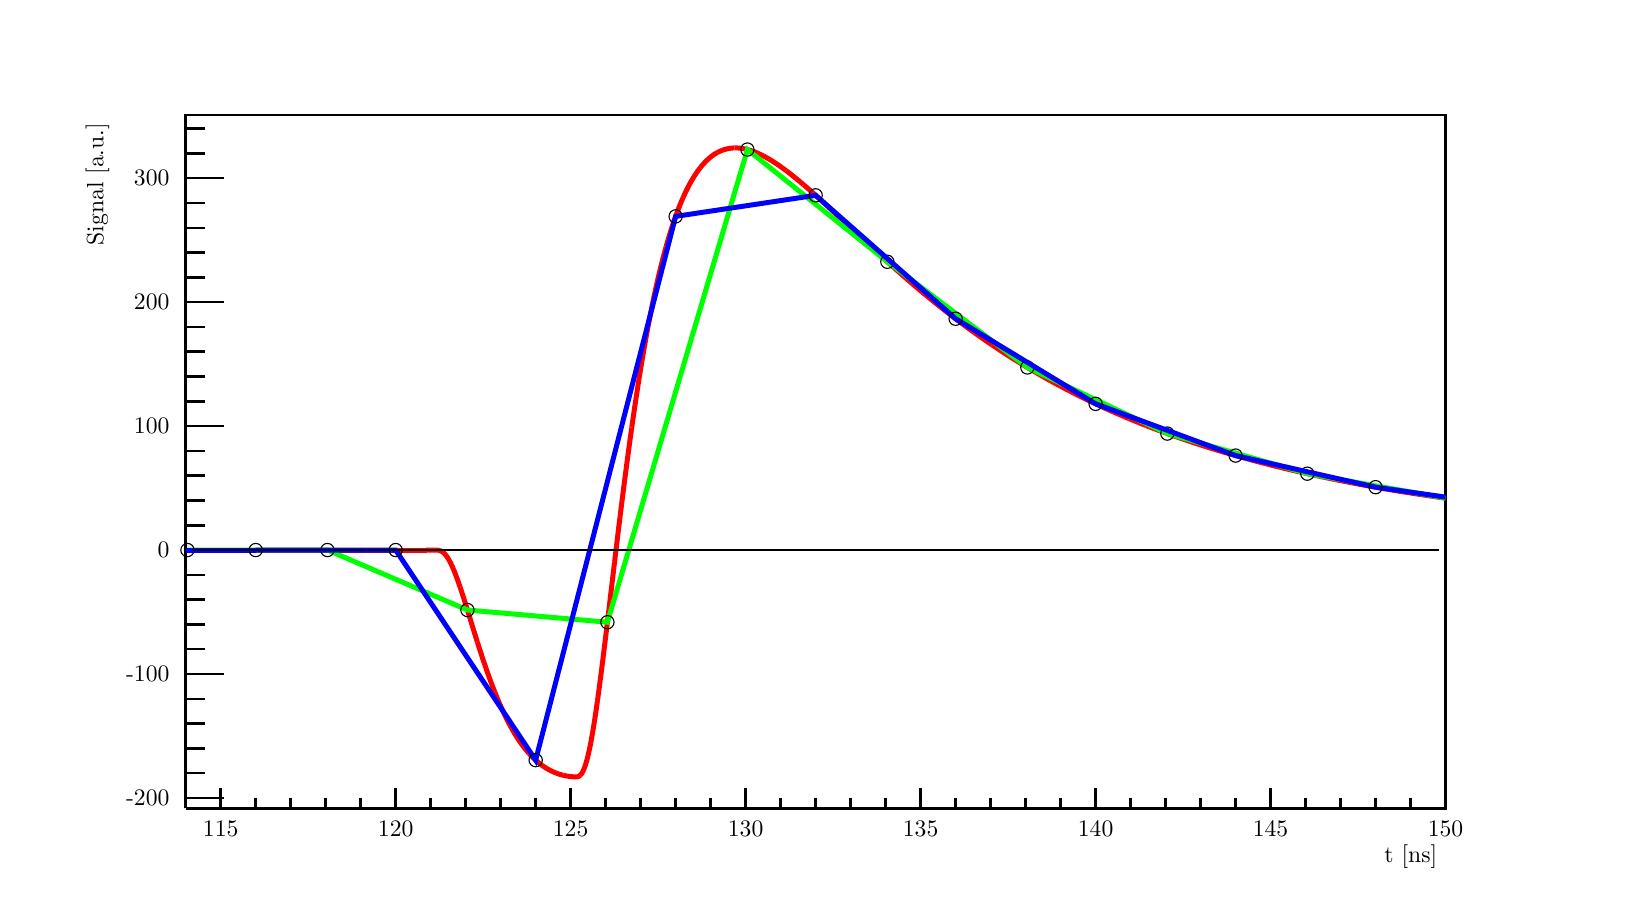
\begin{tikzpicture}
\pgfdeclareplotmark{cross} {
\pgfpathmoveto{\pgfpoint{-0.3\pgfplotmarksize}{\pgfplotmarksize}}
\pgfpathlineto{\pgfpoint{+0.3\pgfplotmarksize}{\pgfplotmarksize}}
\pgfpathlineto{\pgfpoint{+0.3\pgfplotmarksize}{0.3\pgfplotmarksize}}
\pgfpathlineto{\pgfpoint{+1\pgfplotmarksize}{0.3\pgfplotmarksize}}
\pgfpathlineto{\pgfpoint{+1\pgfplotmarksize}{-0.3\pgfplotmarksize}}
\pgfpathlineto{\pgfpoint{+0.3\pgfplotmarksize}{-0.3\pgfplotmarksize}}
\pgfpathlineto{\pgfpoint{+0.3\pgfplotmarksize}{-1.\pgfplotmarksize}}
\pgfpathlineto{\pgfpoint{-0.3\pgfplotmarksize}{-1.\pgfplotmarksize}}
\pgfpathlineto{\pgfpoint{-0.3\pgfplotmarksize}{-0.3\pgfplotmarksize}}
\pgfpathlineto{\pgfpoint{-1.\pgfplotmarksize}{-0.3\pgfplotmarksize}}
\pgfpathlineto{\pgfpoint{-1.\pgfplotmarksize}{0.3\pgfplotmarksize}}
\pgfpathlineto{\pgfpoint{-0.3\pgfplotmarksize}{0.3\pgfplotmarksize}}
\pgfpathclose
\pgfusepathqstroke
}
\pgfdeclareplotmark{cross*} {
\pgfpathmoveto{\pgfpoint{-0.3\pgfplotmarksize}{\pgfplotmarksize}}
\pgfpathlineto{\pgfpoint{+0.3\pgfplotmarksize}{\pgfplotmarksize}}
\pgfpathlineto{\pgfpoint{+0.3\pgfplotmarksize}{0.3\pgfplotmarksize}}
\pgfpathlineto{\pgfpoint{+1\pgfplotmarksize}{0.3\pgfplotmarksize}}
\pgfpathlineto{\pgfpoint{+1\pgfplotmarksize}{-0.3\pgfplotmarksize}}
\pgfpathlineto{\pgfpoint{+0.3\pgfplotmarksize}{-0.3\pgfplotmarksize}}
\pgfpathlineto{\pgfpoint{+0.3\pgfplotmarksize}{-1.\pgfplotmarksize}}
\pgfpathlineto{\pgfpoint{-0.3\pgfplotmarksize}{-1.\pgfplotmarksize}}
\pgfpathlineto{\pgfpoint{-0.3\pgfplotmarksize}{-0.3\pgfplotmarksize}}
\pgfpathlineto{\pgfpoint{-1.\pgfplotmarksize}{-0.3\pgfplotmarksize}}
\pgfpathlineto{\pgfpoint{-1.\pgfplotmarksize}{0.3\pgfplotmarksize}}
\pgfpathlineto{\pgfpoint{-0.3\pgfplotmarksize}{0.3\pgfplotmarksize}}
\pgfpathclose
\pgfusepathqfillstroke
}
\pgfdeclareplotmark{newstar} {
\pgfpathmoveto{\pgfqpoint{0pt}{\pgfplotmarksize}}
\pgfpathlineto{\pgfqpointpolar{44}{0.5\pgfplotmarksize}}
\pgfpathlineto{\pgfqpointpolar{18}{\pgfplotmarksize}}
\pgfpathlineto{\pgfqpointpolar{-20}{0.5\pgfplotmarksize}}
\pgfpathlineto{\pgfqpointpolar{-54}{\pgfplotmarksize}}
\pgfpathlineto{\pgfqpointpolar{-90}{0.5\pgfplotmarksize}}
\pgfpathlineto{\pgfqpointpolar{234}{\pgfplotmarksize}}
\pgfpathlineto{\pgfqpointpolar{198}{0.5\pgfplotmarksize}}
\pgfpathlineto{\pgfqpointpolar{162}{\pgfplotmarksize}}
\pgfpathlineto{\pgfqpointpolar{134}{0.5\pgfplotmarksize}}
\pgfpathclose
\pgfusepathqstroke
}
\pgfdeclareplotmark{newstar*} {
\pgfpathmoveto{\pgfqpoint{0pt}{\pgfplotmarksize}}
\pgfpathlineto{\pgfqpointpolar{44}{0.5\pgfplotmarksize}}
\pgfpathlineto{\pgfqpointpolar{18}{\pgfplotmarksize}}
\pgfpathlineto{\pgfqpointpolar{-20}{0.5\pgfplotmarksize}}
\pgfpathlineto{\pgfqpointpolar{-54}{\pgfplotmarksize}}
\pgfpathlineto{\pgfqpointpolar{-90}{0.5\pgfplotmarksize}}
\pgfpathlineto{\pgfqpointpolar{234}{\pgfplotmarksize}}
\pgfpathlineto{\pgfqpointpolar{198}{0.5\pgfplotmarksize}}
\pgfpathlineto{\pgfqpointpolar{162}{\pgfplotmarksize}}
\pgfpathlineto{\pgfqpointpolar{134}{0.5\pgfplotmarksize}}
\pgfpathclose
\pgfusepathqfillstroke
}
\definecolor{c}{rgb}{1,1,1};
\draw [color=c, fill=c] (0,0) rectangle (20,11.0085);
\draw [color=c, fill=c] (2,1.10085) rectangle (18,9.90762);
\definecolor{c}{rgb}{0,0,0};
\draw [c,line width=0.9] (2,1.10085) -- (2,9.90762) -- (18,9.90762) -- (18,1.10085) -- (2,1.10085);
\definecolor{c}{rgb}{1,1,1};
\draw [color=c, fill=c] (2,1.10085) rectangle (18,9.90762);
\definecolor{c}{rgb}{0,0,0};
\draw [c,line width=0.9] (2,1.10085) -- (2,9.90762) -- (18,9.90762) -- (18,1.10085) -- (2,1.10085);
\definecolor{c}{rgb}{1,0,0};
\draw [c,line width=1.8] (2.00222,4.38131) -- (2.00667,4.38131) -- (2.01111,4.38131) -- (2.01556,4.38131) -- (2.02,4.38131) -- (2.02444,4.38131) -- (2.02889,4.38131) -- (2.03333,4.38131) -- (2.03778,4.38131) -- (2.04222,4.38131) -- (2.04667,4.38131)
 -- (2.05111,4.38131) -- (2.05556,4.38131) -- (2.06,4.38131) -- (2.06444,4.38131) -- (2.06889,4.38131) -- (2.07333,4.38131) -- (2.07778,4.38131) -- (2.08222,4.38131) -- (2.08667,4.38131) -- (2.09111,4.38131) -- (2.09556,4.38131) -- (2.1,4.38131) --
 (2.10444,4.38131) -- (2.10889,4.38131) -- (2.11333,4.38131) -- (2.11778,4.38131) -- (2.12222,4.38131) -- (2.12667,4.38131) -- (2.13111,4.38131) -- (2.13556,4.38131) -- (2.14,4.38131) -- (2.14444,4.38131) -- (2.14889,4.38131) -- (2.15333,4.38131) --
 (2.15778,4.38131) -- (2.16222,4.38131) -- (2.16667,4.38131) -- (2.17111,4.38131) -- (2.17556,4.38131) -- (2.18,4.38131) -- (2.18444,4.38131) -- (2.18889,4.38131) -- (2.19333,4.38131) -- (2.19778,4.38131) -- (2.20222,4.38131) -- (2.20667,4.38131) --
 (2.21111,4.38131) -- (2.21556,4.38131) -- (2.22,4.38131);
\draw [c,line width=1.8] (2.22,4.38131) -- (2.22444,4.38131) -- (2.22889,4.38131) -- (2.23333,4.38131) -- (2.23778,4.38131) -- (2.24222,4.38131) -- (2.24667,4.38131) -- (2.25111,4.38131) -- (2.25556,4.38131) -- (2.26,4.38131) -- (2.26444,4.38131) --
 (2.26889,4.38131) -- (2.27333,4.38131) -- (2.27778,4.38131) -- (2.28222,4.38131) -- (2.28667,4.38131) -- (2.29111,4.38131) -- (2.29556,4.38131) -- (2.3,4.38131) -- (2.30444,4.38131) -- (2.30889,4.38131) -- (2.31333,4.38131) -- (2.31778,4.38131) --
 (2.32222,4.38131) -- (2.32667,4.38131) -- (2.33111,4.38131) -- (2.33556,4.38131) -- (2.34,4.38131) -- (2.34444,4.38131) -- (2.34889,4.38131) -- (2.35333,4.38131) -- (2.35778,4.38131) -- (2.36222,4.38131) -- (2.36667,4.38131) -- (2.37111,4.38131) --
 (2.37556,4.38131) -- (2.38,4.38131) -- (2.38444,4.38131) -- (2.38889,4.38131) -- (2.39333,4.38131) -- (2.39778,4.38131) -- (2.40222,4.38131) -- (2.40667,4.38131) -- (2.41111,4.38131) -- (2.41556,4.38131) -- (2.42,4.38131) -- (2.42444,4.38131) --
 (2.42889,4.38131) -- (2.43333,4.38131) -- (2.43778,4.38131);
\draw [c,line width=1.8] (2.43778,4.38131) -- (2.44222,4.38131) -- (2.44667,4.38131) -- (2.45111,4.38131) -- (2.45556,4.38131) -- (2.46,4.38131) -- (2.46444,4.38131) -- (2.46889,4.38131) -- (2.47333,4.38131) -- (2.47778,4.38131) -- (2.48222,4.38131)
 -- (2.48667,4.38131) -- (2.49111,4.38131) -- (2.49556,4.38131) -- (2.5,4.38131) -- (2.50444,4.38131) -- (2.50889,4.38131) -- (2.51333,4.38131) -- (2.51778,4.38131) -- (2.52222,4.38131) -- (2.52667,4.38131) -- (2.53111,4.38131) -- (2.53556,4.38131)
 -- (2.54,4.38131) -- (2.54444,4.38131) -- (2.54889,4.38131) -- (2.55333,4.38131) -- (2.55778,4.38131) -- (2.56222,4.38131) -- (2.56667,4.38131) -- (2.57111,4.38131) -- (2.57556,4.38131) -- (2.58,4.38131) -- (2.58444,4.38131) -- (2.58889,4.38131) --
 (2.59333,4.38131) -- (2.59778,4.38131) -- (2.60222,4.38131) -- (2.60667,4.38131) -- (2.61111,4.38131) -- (2.61556,4.38131) -- (2.62,4.38131) -- (2.62444,4.38131) -- (2.62889,4.38131) -- (2.63333,4.38131) -- (2.63778,4.38131) -- (2.64222,4.38131) --
 (2.64667,4.38131) -- (2.65111,4.38131) -- (2.65556,4.38131);
\draw [c,line width=1.8] (2.65556,4.38131) -- (2.66,4.38131) -- (2.66444,4.38131) -- (2.66889,4.38131) -- (2.67333,4.38131) -- (2.67778,4.38131) -- (2.68222,4.38131) -- (2.68667,4.38131) -- (2.69111,4.38131) -- (2.69556,4.38131) -- (2.7,4.38131) --
 (2.70444,4.38131) -- (2.70889,4.38131) -- (2.71333,4.38131) -- (2.71778,4.38131) -- (2.72222,4.38131) -- (2.72667,4.38131) -- (2.73111,4.38131) -- (2.73556,4.38131) -- (2.74,4.38131) -- (2.74444,4.38131) -- (2.74889,4.38131) -- (2.75333,4.38131) --
 (2.75778,4.38131) -- (2.76222,4.38131) -- (2.76667,4.38131) -- (2.77111,4.38131) -- (2.77556,4.38131) -- (2.78,4.38131) -- (2.78444,4.38131) -- (2.78889,4.38131) -- (2.79333,4.38131) -- (2.79778,4.38131) -- (2.80222,4.38131) -- (2.80667,4.38131) --
 (2.81111,4.38131) -- (2.81556,4.38131) -- (2.82,4.38131) -- (2.82444,4.38131) -- (2.82889,4.38131) -- (2.83333,4.38131) -- (2.83778,4.38131) -- (2.84222,4.38131) -- (2.84667,4.38131) -- (2.85111,4.38131) -- (2.85556,4.38131) -- (2.86,4.38131) --
 (2.86444,4.38131) -- (2.86889,4.38131) -- (2.87333,4.38131);
\draw [c,line width=1.8] (2.87333,4.38131) -- (2.87778,4.38131) -- (2.88222,4.38131) -- (2.88667,4.38131) -- (2.89111,4.38131) -- (2.89556,4.38131) -- (2.9,4.38131) -- (2.90444,4.38131) -- (2.90889,4.38131) -- (2.91333,4.38131) -- (2.91778,4.38131)
 -- (2.92222,4.38131) -- (2.92667,4.38131) -- (2.93111,4.38131) -- (2.93556,4.38131) -- (2.94,4.38131) -- (2.94444,4.38131) -- (2.94889,4.38131) -- (2.95333,4.38131) -- (2.95778,4.38131) -- (2.96222,4.38131) -- (2.96667,4.38131) -- (2.97111,4.38131)
 -- (2.97556,4.38131) -- (2.98,4.38131) -- (2.98444,4.38131) -- (2.98889,4.38131) -- (2.99333,4.38131) -- (2.99778,4.38131) -- (3.00222,4.38131) -- (3.00667,4.38131) -- (3.01111,4.38131) -- (3.01556,4.38131) -- (3.02,4.38131) -- (3.02444,4.38131) --
 (3.02889,4.38131) -- (3.03333,4.38131) -- (3.03778,4.38131) -- (3.04222,4.38131) -- (3.04667,4.38131) -- (3.05111,4.38131) -- (3.05556,4.38131) -- (3.06,4.38131) -- (3.06444,4.38131) -- (3.06889,4.38131) -- (3.07333,4.38131) -- (3.07778,4.38131) --
 (3.08222,4.38131) -- (3.08667,4.38131) -- (3.09111,4.38131);
\draw [c,line width=1.8] (3.09111,4.38131) -- (3.09556,4.38131) -- (3.1,4.38131) -- (3.10444,4.38131) -- (3.10889,4.38131) -- (3.11333,4.38131) -- (3.11778,4.38131) -- (3.12222,4.38131) -- (3.12667,4.38131) -- (3.13111,4.38131) -- (3.13556,4.38131)
 -- (3.14,4.38131) -- (3.14444,4.38131) -- (3.14889,4.38131) -- (3.15333,4.38131) -- (3.15778,4.38131) -- (3.16222,4.38131) -- (3.16667,4.38131) -- (3.17111,4.38131) -- (3.17556,4.38131) -- (3.18,4.38131) -- (3.18444,4.38131) -- (3.18889,4.38131) --
 (3.19333,4.38131) -- (3.19778,4.38131) -- (3.20222,4.38131) -- (3.20667,4.38131) -- (3.21111,4.38131) -- (3.21556,4.38131) -- (3.22,4.38131) -- (3.22444,4.38131) -- (3.22889,4.38131) -- (3.23333,4.38131) -- (3.23778,4.38131) -- (3.24222,4.38131) --
 (3.24667,4.38131) -- (3.25111,4.38131) -- (3.25556,4.38131) -- (3.26,4.38131) -- (3.26444,4.38131) -- (3.26889,4.38131) -- (3.27333,4.38131) -- (3.27778,4.38131) -- (3.28222,4.38131) -- (3.28667,4.38131) -- (3.29111,4.38131) -- (3.29556,4.38131) --
 (3.3,4.38131) -- (3.30444,4.38131) -- (3.30889,4.38131);
\draw [c,line width=1.8] (3.30889,4.38131) -- (3.31333,4.38131) -- (3.31778,4.38131) -- (3.32222,4.38131) -- (3.32667,4.38131) -- (3.33111,4.38131) -- (3.33556,4.38131) -- (3.34,4.38131) -- (3.34444,4.38131) -- (3.34889,4.38131) -- (3.35333,4.38131)
 -- (3.35778,4.38131) -- (3.36222,4.38131) -- (3.36667,4.38131) -- (3.37111,4.38131) -- (3.37556,4.38131) -- (3.38,4.38131) -- (3.38444,4.38131) -- (3.38889,4.38131) -- (3.39333,4.38131) -- (3.39778,4.38131) -- (3.40222,4.38131) -- (3.40667,4.38131)
 -- (3.41111,4.38131) -- (3.41556,4.38131) -- (3.42,4.38131) -- (3.42444,4.38131) -- (3.42889,4.38131) -- (3.43333,4.38131) -- (3.43778,4.38131) -- (3.44222,4.38131) -- (3.44667,4.38131) -- (3.45111,4.38131) -- (3.45556,4.38131) -- (3.46,4.38131) --
 (3.46444,4.38131) -- (3.46889,4.38131) -- (3.47333,4.38131) -- (3.47778,4.38131) -- (3.48222,4.38131) -- (3.48667,4.38131) -- (3.49111,4.38131) -- (3.49556,4.38131) -- (3.5,4.38131) -- (3.50444,4.38131) -- (3.50889,4.38131) -- (3.51333,4.38131) --
 (3.51778,4.38131) -- (3.52222,4.38131) -- (3.52667,4.38131);
\draw [c,line width=1.8] (3.52667,4.38131) -- (3.53111,4.38131) -- (3.53556,4.38131) -- (3.54,4.38131) -- (3.54444,4.38131) -- (3.54889,4.38131) -- (3.55333,4.38131) -- (3.55778,4.38131) -- (3.56222,4.38131) -- (3.56667,4.38131) -- (3.57111,4.38131)
 -- (3.57556,4.38131) -- (3.58,4.38131) -- (3.58444,4.38131) -- (3.58889,4.38131) -- (3.59333,4.38131) -- (3.59778,4.38131) -- (3.60222,4.38131) -- (3.60667,4.38131) -- (3.61111,4.38131) -- (3.61556,4.38131) -- (3.62,4.38131) -- (3.62444,4.38131) --
 (3.62889,4.38131) -- (3.63333,4.38131) -- (3.63778,4.38131) -- (3.64222,4.38131) -- (3.64667,4.38131) -- (3.65111,4.38131) -- (3.65556,4.38131) -- (3.66,4.38131) -- (3.66444,4.38131) -- (3.66889,4.38131) -- (3.67333,4.38131) -- (3.67778,4.38131) --
 (3.68222,4.38131) -- (3.68667,4.38131) -- (3.69111,4.38131) -- (3.69556,4.38131) -- (3.7,4.38131) -- (3.70444,4.38131) -- (3.70889,4.38131) -- (3.71333,4.38131) -- (3.71778,4.38131) -- (3.72222,4.38131) -- (3.72667,4.38131) -- (3.73111,4.38131) --
 (3.73556,4.38131) -- (3.74,4.38131) -- (3.74444,4.38131);
\draw [c,line width=1.8] (3.74444,4.38131) -- (3.74889,4.38131) -- (3.75333,4.38131) -- (3.75778,4.38131) -- (3.76222,4.38131) -- (3.76667,4.38131) -- (3.77111,4.38131) -- (3.77556,4.38131) -- (3.78,4.38131) -- (3.78444,4.38131) -- (3.78889,4.38131)
 -- (3.79333,4.38131) -- (3.79778,4.38131) -- (3.80222,4.38131) -- (3.80667,4.38131) -- (3.81111,4.38131) -- (3.81556,4.38131) -- (3.82,4.38131) -- (3.82444,4.38131) -- (3.82889,4.38131) -- (3.83333,4.38131) -- (3.83778,4.38131) -- (3.84222,4.38131)
 -- (3.84667,4.38131) -- (3.85111,4.38131) -- (3.85556,4.38131) -- (3.86,4.38131) -- (3.86444,4.38131) -- (3.86889,4.38131) -- (3.87333,4.38131) -- (3.87778,4.38131) -- (3.88222,4.38131) -- (3.88667,4.38131) -- (3.89111,4.38131) -- (3.89556,4.38131)
 -- (3.9,4.38131) -- (3.90444,4.38131) -- (3.90889,4.38131) -- (3.91333,4.38131) -- (3.91778,4.38131) -- (3.92222,4.38131) -- (3.92667,4.38131) -- (3.93111,4.38131) -- (3.93556,4.38131) -- (3.94,4.38131) -- (3.94444,4.38131) -- (3.94889,4.38131) --
 (3.95333,4.38131) -- (3.95778,4.38131) -- (3.96222,4.38131);
\draw [c,line width=1.8] (3.96222,4.38131) -- (3.96667,4.38131) -- (3.97111,4.38131) -- (3.97556,4.38131) -- (3.98,4.38131) -- (3.98444,4.38131) -- (3.98889,4.38131) -- (3.99333,4.38131) -- (3.99778,4.38131) -- (4.00222,4.38131) -- (4.00667,4.38131)
 -- (4.01111,4.38131) -- (4.01556,4.38131) -- (4.02,4.38131) -- (4.02444,4.38131) -- (4.02889,4.38131) -- (4.03333,4.38131) -- (4.03778,4.38131) -- (4.04222,4.38131) -- (4.04667,4.38131) -- (4.05111,4.38131) -- (4.05556,4.38131) -- (4.06,4.38131) --
 (4.06444,4.38131) -- (4.06889,4.38131) -- (4.07333,4.38131) -- (4.07778,4.38131) -- (4.08222,4.38131) -- (4.08667,4.38131) -- (4.09111,4.38131) -- (4.09556,4.38131) -- (4.1,4.38131) -- (4.10444,4.38131) -- (4.10889,4.38131) -- (4.11333,4.38131) --
 (4.11778,4.38131) -- (4.12222,4.38131) -- (4.12667,4.38131) -- (4.13111,4.38131) -- (4.13556,4.38131) -- (4.14,4.38131) -- (4.14444,4.38131) -- (4.14889,4.38131) -- (4.15333,4.38131) -- (4.15778,4.38131) -- (4.16222,4.38131) -- (4.16667,4.38131) --
 (4.17111,4.38131) -- (4.17556,4.38131) -- (4.18,4.38131);
\draw [c,line width=1.8] (4.18,4.38131) -- (4.18444,4.38131) -- (4.18889,4.38131) -- (4.19333,4.38131) -- (4.19778,4.38131) -- (4.20222,4.38131) -- (4.20667,4.38131) -- (4.21111,4.38131) -- (4.21556,4.38131) -- (4.22,4.38131) -- (4.22444,4.38131) --
 (4.22889,4.38131) -- (4.23333,4.38131) -- (4.23778,4.38131) -- (4.24222,4.38131) -- (4.24667,4.38131) -- (4.25111,4.38131) -- (4.25556,4.38131) -- (4.26,4.38131) -- (4.26444,4.38131) -- (4.26889,4.38131) -- (4.27333,4.38131) -- (4.27778,4.38131) --
 (4.28222,4.38131) -- (4.28667,4.38131) -- (4.29111,4.38131) -- (4.29556,4.38131) -- (4.3,4.38131) -- (4.30444,4.38131) -- (4.30889,4.38131) -- (4.31333,4.38131) -- (4.31778,4.38131) -- (4.32222,4.38131) -- (4.32667,4.38131) -- (4.33111,4.38131) --
 (4.33556,4.38131) -- (4.34,4.38131) -- (4.34444,4.38131) -- (4.34889,4.38131) -- (4.35333,4.38131) -- (4.35778,4.38131) -- (4.36222,4.38131) -- (4.36667,4.38131) -- (4.37111,4.38131) -- (4.37556,4.38131) -- (4.38,4.38131) -- (4.38444,4.38131) --
 (4.38889,4.38131) -- (4.39333,4.38131) -- (4.39778,4.38131);
\draw [c,line width=1.8] (4.39778,4.38131) -- (4.40222,4.38131) -- (4.40667,4.38131) -- (4.41111,4.38131) -- (4.41556,4.38131) -- (4.42,4.38131) -- (4.42444,4.38131) -- (4.42889,4.38131) -- (4.43333,4.38131) -- (4.43778,4.38131) -- (4.44222,4.38131)
 -- (4.44667,4.38131) -- (4.45111,4.38131) -- (4.45556,4.38131) -- (4.46,4.38131) -- (4.46444,4.38131) -- (4.46889,4.38131) -- (4.47333,4.38131) -- (4.47778,4.38131) -- (4.48222,4.38131) -- (4.48667,4.38131) -- (4.49111,4.38131) -- (4.49556,4.38131)
 -- (4.5,4.38131) -- (4.50444,4.38131) -- (4.50889,4.38131) -- (4.51333,4.38131) -- (4.51778,4.38131) -- (4.52222,4.38131) -- (4.52667,4.38131) -- (4.53111,4.38131) -- (4.53556,4.38131) -- (4.54,4.38131) -- (4.54444,4.38131) -- (4.54889,4.38131) --
 (4.55333,4.38131) -- (4.55778,4.38131) -- (4.56222,4.38131) -- (4.56667,4.38131) -- (4.57111,4.38131) -- (4.57556,4.38131) -- (4.58,4.38131) -- (4.58444,4.38131) -- (4.58889,4.38131) -- (4.59333,4.38131) -- (4.59778,4.38131) -- (4.60222,4.38131) --
 (4.60667,4.38131) -- (4.61111,4.38131) -- (4.61556,4.38131);
\draw [c,line width=1.8] (4.61556,4.38131) -- (4.62,4.38131) -- (4.62444,4.38131) -- (4.62889,4.38131) -- (4.63333,4.38131) -- (4.63778,4.38131) -- (4.64222,4.38131) -- (4.64667,4.38131) -- (4.65111,4.38131) -- (4.65556,4.38131) -- (4.66,4.38131) --
 (4.66444,4.38131) -- (4.66889,4.38131) -- (4.67333,4.38131) -- (4.67778,4.38131) -- (4.68222,4.38131) -- (4.68667,4.38131) -- (4.69111,4.38131) -- (4.69556,4.38131) -- (4.7,4.38131) -- (4.70444,4.38131) -- (4.70889,4.38131) -- (4.71333,4.38131) --
 (4.71778,4.38131) -- (4.72222,4.38131) -- (4.72667,4.38131) -- (4.73111,4.38131) -- (4.73556,4.38131) -- (4.74,4.38131) -- (4.74444,4.38131) -- (4.74889,4.38131) -- (4.75333,4.38131) -- (4.75778,4.38131) -- (4.76222,4.38131) -- (4.76667,4.38131) --
 (4.77111,4.38131) -- (4.77556,4.38131) -- (4.78,4.38131) -- (4.78444,4.38131) -- (4.78889,4.38131) -- (4.79333,4.38131) -- (4.79778,4.38131) -- (4.80222,4.38131) -- (4.80667,4.38131) -- (4.81111,4.38131) -- (4.81556,4.38131) -- (4.82,4.38131) --
 (4.82444,4.38131) -- (4.82889,4.38131) -- (4.83333,4.38131);
\draw [c,line width=1.8] (4.83333,4.38131) -- (4.83778,4.38131) -- (4.84222,4.38131) -- (4.84667,4.38131) -- (4.85111,4.38131) -- (4.85556,4.38131) -- (4.86,4.38131) -- (4.86444,4.38131) -- (4.86889,4.38131) -- (4.87333,4.38131) -- (4.87778,4.38131)
 -- (4.88222,4.38131) -- (4.88667,4.38131) -- (4.89111,4.38131) -- (4.89556,4.38131) -- (4.9,4.38131) -- (4.90444,4.38131) -- (4.90889,4.38131) -- (4.91333,4.38131) -- (4.91778,4.38131) -- (4.92222,4.38131) -- (4.92667,4.38131) -- (4.93111,4.38131)
 -- (4.93556,4.38131) -- (4.94,4.38131) -- (4.94444,4.38131) -- (4.94889,4.38131) -- (4.95333,4.38131) -- (4.95778,4.38131) -- (4.96222,4.38131) -- (4.96667,4.38131) -- (4.97111,4.38131) -- (4.97556,4.38131) -- (4.98,4.38131) -- (4.98444,4.38131) --
 (4.98889,4.38131) -- (4.99333,4.38131) -- (4.99778,4.38131) -- (5.00222,4.38131) -- (5.00667,4.38131) -- (5.01111,4.38131) -- (5.01556,4.38131) -- (5.02,4.38131) -- (5.02444,4.38131) -- (5.02889,4.38131) -- (5.03333,4.38131) -- (5.03778,4.38131) --
 (5.04222,4.38131) -- (5.04667,4.38131) -- (5.05111,4.38131);
\draw [c,line width=1.8] (5.05111,4.38131) -- (5.05556,4.38131) -- (5.06,4.38131) -- (5.06444,4.38131) -- (5.06889,4.38131) -- (5.07333,4.38131) -- (5.07778,4.38131) -- (5.08222,4.38131) -- (5.08667,4.38131) -- (5.09111,4.38131) -- (5.09556,4.38131)
 -- (5.1,4.38131) -- (5.10444,4.38131) -- (5.10889,4.38131) -- (5.11333,4.38131) -- (5.11778,4.38131) -- (5.12222,4.38131) -- (5.12667,4.38131) -- (5.13111,4.38131) -- (5.13556,4.38131) -- (5.14,4.38131) -- (5.14444,4.38131) -- (5.14889,4.38131) --
 (5.15333,4.38131) -- (5.15778,4.38131) -- (5.16222,4.3813) -- (5.16667,4.38129) -- (5.17111,4.38126) -- (5.17556,4.3812) -- (5.18,4.38111) -- (5.18444,4.38097) -- (5.18889,4.38077) -- (5.19333,4.38049) -- (5.19778,4.38012) -- (5.20222,4.37965) --
 (5.20667,4.37906) -- (5.21111,4.37833) -- (5.21556,4.37746) -- (5.22,4.37642) -- (5.22444,4.37522) -- (5.22889,4.37383) -- (5.23333,4.37225) -- (5.23778,4.37046) -- (5.24222,4.36846) -- (5.24667,4.36624) -- (5.25111,4.36379) -- (5.25556,4.36111) --
 (5.26,4.35818) -- (5.26444,4.35501) -- (5.26889,4.35159);
\draw [c,line width=1.8] (5.26889,4.35159) -- (5.27333,4.34792) -- (5.27778,4.34399) -- (5.28222,4.3398) -- (5.28667,4.33535) -- (5.29111,4.33064) -- (5.29556,4.32566) -- (5.3,4.32043) -- (5.30444,4.31494) -- (5.30889,4.30918) -- (5.31333,4.30317) --
 (5.31778,4.2969) -- (5.32222,4.29037) -- (5.32667,4.28359) -- (5.33111,4.27656) -- (5.33556,4.26929) -- (5.34,4.26177) -- (5.34444,4.254) -- (5.34889,4.24601) -- (5.35333,4.23777) -- (5.35778,4.22931) -- (5.36222,4.22062) -- (5.36667,4.21172) --
 (5.37111,4.20259) -- (5.37556,4.19325) -- (5.38,4.18371) -- (5.38444,4.17396) -- (5.38889,4.16401) -- (5.39333,4.15387) -- (5.39778,4.14353) -- (5.40222,4.13302) -- (5.40667,4.12232) -- (5.41111,4.11145) -- (5.41556,4.1004) -- (5.42,4.08919) --
 (5.42444,4.07782) -- (5.42889,4.0663) -- (5.43333,4.05462) -- (5.43778,4.0428) -- (5.44222,4.03083) -- (5.44667,4.01873) -- (5.45111,4.00649) -- (5.45556,3.99412) -- (5.46,3.98163) -- (5.46444,3.96903) -- (5.46889,3.9563) -- (5.47333,3.94347) --
 (5.47778,3.93053) -- (5.48222,3.91749) -- (5.48667,3.90435);
\draw [c,line width=1.8] (5.48667,3.90435) -- (5.49111,3.89111) -- (5.49556,3.87779) -- (5.5,3.86438) -- (5.50444,3.85089) -- (5.50889,3.83733) -- (5.51333,3.82369) -- (5.51778,3.80998) -- (5.52222,3.7962) -- (5.52667,3.78236) -- (5.53111,3.76846) --
 (5.53556,3.75451) -- (5.54,3.7405) -- (5.54444,3.72645) -- (5.54889,3.71235) -- (5.55333,3.69821) -- (5.55778,3.68403) -- (5.56222,3.66981) -- (5.56667,3.65556) -- (5.57111,3.64128) -- (5.57556,3.62698) -- (5.58,3.61265) -- (5.58444,3.5983) --
 (5.58889,3.58393) -- (5.59333,3.56954) -- (5.59778,3.55515) -- (5.60222,3.54074) -- (5.60667,3.52632) -- (5.61111,3.5119) -- (5.61556,3.49748) -- (5.62,3.48305) -- (5.62444,3.46863) -- (5.62889,3.45421) -- (5.63333,3.4398) -- (5.63778,3.42539) --
 (5.64222,3.411) -- (5.64667,3.39662) -- (5.65111,3.38225) -- (5.65556,3.3679) -- (5.66,3.35356) -- (5.66444,3.33925) -- (5.66889,3.32496) -- (5.67333,3.31069) -- (5.67778,3.29645) -- (5.68222,3.28223) -- (5.68667,3.26804) -- (5.69111,3.25388) --
 (5.69556,3.23976) -- (5.7,3.22566) -- (5.70444,3.2116);
\draw [c,line width=1.8] (5.70444,3.2116) -- (5.70889,3.19758) -- (5.71333,3.18359) -- (5.71778,3.16964) -- (5.72222,3.15573) -- (5.72667,3.14186) -- (5.73111,3.12804) -- (5.73556,3.11426) -- (5.74,3.10052) -- (5.74444,3.08683) -- (5.74889,3.07318)
 -- (5.75333,3.05958) -- (5.75778,3.04603) -- (5.76222,3.03253) -- (5.76667,3.01908) -- (5.77111,3.00568) -- (5.77556,2.99234) -- (5.78,2.97904) -- (5.78444,2.9658) -- (5.78889,2.95262) -- (5.79333,2.93949) -- (5.79778,2.92642) -- (5.80222,2.9134) --
 (5.80667,2.90044) -- (5.81111,2.88754) -- (5.81556,2.8747) -- (5.82,2.86192) -- (5.82444,2.8492) -- (5.82889,2.83654) -- (5.83333,2.82394) -- (5.83778,2.8114) -- (5.84222,2.79892) -- (5.84667,2.78651) -- (5.85111,2.77416) -- (5.85556,2.76187) --
 (5.86,2.74965) -- (5.86444,2.73749) -- (5.86889,2.7254) -- (5.87333,2.71337) -- (5.87778,2.70141) -- (5.88222,2.68951) -- (5.88667,2.67768) -- (5.89111,2.66591) -- (5.89556,2.65421) -- (5.9,2.64258) -- (5.90444,2.63102) -- (5.90889,2.61952) --
 (5.91333,2.60809) -- (5.91778,2.59673) -- (5.92222,2.58544);
\draw [c,line width=1.8] (5.92222,2.58544) -- (5.92667,2.57421) -- (5.93111,2.56305) -- (5.93556,2.55197) -- (5.94,2.54095) -- (5.94444,2.52999) -- (5.94889,2.51911) -- (5.95333,2.5083) -- (5.95778,2.49755) -- (5.96222,2.48688) -- (5.96667,2.47627)
 -- (5.97111,2.46573) -- (5.97556,2.45526) -- (5.98,2.44486) -- (5.98444,2.43453) -- (5.98889,2.42427) -- (5.99333,2.41408) -- (5.99778,2.40396) -- (6.00222,2.39391) -- (6.00667,2.38392) -- (6.01111,2.37401) -- (6.01556,2.36416) -- (6.02,2.35438) --
 (6.02444,2.34468) -- (6.02889,2.33504) -- (6.03333,2.32547) -- (6.03778,2.31597) -- (6.04222,2.30653) -- (6.04667,2.29717) -- (6.05111,2.28787) -- (6.05556,2.27865) -- (6.06,2.26949) -- (6.06444,2.2604) -- (6.06889,2.25137) -- (6.07333,2.24242) --
 (6.07778,2.23353) -- (6.08222,2.22471) -- (6.08667,2.21596) -- (6.09111,2.20727) -- (6.09556,2.19866) -- (6.1,2.1901) -- (6.10444,2.18162) -- (6.10889,2.1732) -- (6.11333,2.16485) -- (6.11778,2.15657) -- (6.12222,2.14835) -- (6.12667,2.1402) --
 (6.13111,2.13211) -- (6.13556,2.12409) -- (6.14,2.11613);
\draw [c,line width=1.8] (6.14,2.11613) -- (6.14444,2.10824) -- (6.14889,2.10041) -- (6.15333,2.09265) -- (6.15778,2.08496) -- (6.16222,2.07732) -- (6.16667,2.06975) -- (6.17111,2.06225) -- (6.17556,2.05481) -- (6.18,2.04743) -- (6.18444,2.04011) --
 (6.18889,2.03286) -- (6.19333,2.02567) -- (6.19778,2.01855) -- (6.20222,2.01148) -- (6.20667,2.00448) -- (6.21111,1.99754) -- (6.21556,1.99066) -- (6.22,1.98384) -- (6.22444,1.97708) -- (6.22889,1.97039) -- (6.23333,1.96375) -- (6.23778,1.95717) --
 (6.24222,1.95066) -- (6.24667,1.9442) -- (6.25111,1.9378) -- (6.25556,1.93147) -- (6.26,1.92519) -- (6.26444,1.91897) -- (6.26889,1.91281) -- (6.27333,1.9067) -- (6.27778,1.90066) -- (6.28222,1.89467) -- (6.28667,1.88874) -- (6.29111,1.88286) --
 (6.29556,1.87705) -- (6.3,1.87129) -- (6.30444,1.86558) -- (6.30889,1.85993) -- (6.31333,1.85434) -- (6.31778,1.8488) -- (6.32222,1.84332) -- (6.32667,1.8379) -- (6.33111,1.83252) -- (6.33556,1.82721) -- (6.34,1.82194) -- (6.34444,1.81673) --
 (6.34889,1.81158) -- (6.35333,1.80647) -- (6.35778,1.80142);
\draw [c,line width=1.8] (6.35778,1.80142) -- (6.36222,1.79643) -- (6.36667,1.79148) -- (6.37111,1.78659) -- (6.37556,1.78175) -- (6.38,1.77696) -- (6.38444,1.77222) -- (6.38889,1.76754) -- (6.39333,1.7629) -- (6.39778,1.75832) -- (6.40222,1.75378)
 -- (6.40667,1.7493) -- (6.41111,1.74486) -- (6.41556,1.74048) -- (6.42,1.73614) -- (6.42444,1.73186) -- (6.42889,1.72762) -- (6.43333,1.72343) -- (6.43778,1.71929) -- (6.44222,1.71519) -- (6.44667,1.71115) -- (6.45111,1.70715) -- (6.45556,1.70319)
 -- (6.46,1.69929) -- (6.46444,1.69543) -- (6.46889,1.69162) -- (6.47333,1.68785) -- (6.47778,1.68413) -- (6.48222,1.68046) -- (6.48667,1.67683) -- (6.49111,1.67324) -- (6.49556,1.6697) -- (6.5,1.66621) -- (6.50444,1.66276) -- (6.50889,1.65935) --
 (6.51333,1.65599) -- (6.51778,1.65266) -- (6.52222,1.64939) -- (6.52667,1.64615) -- (6.53111,1.64296) -- (6.53556,1.63981) -- (6.54,1.63671) -- (6.54444,1.63364) -- (6.54889,1.63062) -- (6.55333,1.62763) -- (6.55778,1.62469) -- (6.56222,1.62179) --
 (6.56667,1.61893) -- (6.57111,1.61611) -- (6.57556,1.61334);
\draw [c,line width=1.8] (6.57556,1.61334) -- (6.58,1.6106) -- (6.58444,1.6079) -- (6.58889,1.60524) -- (6.59333,1.60262) -- (6.59778,1.60003) -- (6.60222,1.59749) -- (6.60667,1.59499) -- (6.61111,1.59252) -- (6.61556,1.59009) -- (6.62,1.5877) --
 (6.62444,1.58535) -- (6.62889,1.58303) -- (6.63333,1.58075) -- (6.63778,1.57851) -- (6.64222,1.5763) -- (6.64667,1.57414) -- (6.65111,1.572) -- (6.65556,1.5699) -- (6.66,1.56784) -- (6.66444,1.56582) -- (6.66889,1.56383) -- (6.67333,1.56187) --
 (6.67778,1.55995) -- (6.68222,1.55806) -- (6.68667,1.55621) -- (6.69111,1.55439) -- (6.69556,1.5526) -- (6.7,1.55085) -- (6.70444,1.54914) -- (6.70889,1.54745) -- (6.71333,1.5458) -- (6.71778,1.54418) -- (6.72222,1.54259) -- (6.72667,1.54104) --
 (6.73111,1.53952) -- (6.73556,1.53803) -- (6.74,1.53657) -- (6.74444,1.53514) -- (6.74889,1.53375) -- (6.75333,1.53238) -- (6.75778,1.53105) -- (6.76222,1.52975) -- (6.76667,1.52847) -- (6.77111,1.52723) -- (6.77556,1.52602) -- (6.78,1.52484) --
 (6.78444,1.52369) -- (6.78889,1.52256) -- (6.79333,1.52147);
\draw [c,line width=1.8] (6.79333,1.52147) -- (6.79778,1.5204) -- (6.80222,1.51937) -- (6.80667,1.51836) -- (6.81111,1.51738) -- (6.81556,1.51643) -- (6.82,1.51551) -- (6.82444,1.51461) -- (6.82889,1.51375) -- (6.83333,1.51291) -- (6.83778,1.51209)
 -- (6.84222,1.51131) -- (6.84667,1.51055) -- (6.85111,1.50982) -- (6.85556,1.50912) -- (6.86,1.50844) -- (6.86444,1.50779) -- (6.86889,1.50716) -- (6.87333,1.50656) -- (6.87778,1.50598) -- (6.88222,1.50544) -- (6.88667,1.50491) -- (6.89111,1.50441)
 -- (6.89556,1.50394) -- (6.9,1.50349) -- (6.90444,1.50307) -- (6.90889,1.50267) -- (6.91333,1.50229) -- (6.91778,1.50194) -- (6.92222,1.50161) -- (6.92667,1.50131) -- (6.93111,1.50103) -- (6.93556,1.50078) -- (6.94,1.50056) -- (6.94444,1.50038) --
 (6.94889,1.50027) -- (6.95333,1.50025) -- (6.95778,1.50033) -- (6.96222,1.50057) -- (6.96667,1.50097) -- (6.97111,1.50159) -- (6.97556,1.50246) -- (6.98,1.50361) -- (6.98444,1.50509) -- (6.98889,1.50691) -- (6.99333,1.50913) -- (6.99778,1.51176) --
 (7.00222,1.51485) -- (7.00667,1.51842) -- (7.01111,1.52249);
\draw [c,line width=1.8] (7.01111,1.52249) -- (7.01556,1.52709) -- (7.02,1.53225) -- (7.02444,1.53798) -- (7.02889,1.5443) -- (7.03333,1.55123) -- (7.03778,1.55878) -- (7.04222,1.56697) -- (7.04667,1.5758) -- (7.05111,1.58528) -- (7.05556,1.59543) --
 (7.06,1.60623) -- (7.06444,1.61771) -- (7.06889,1.62986) -- (7.07333,1.64268) -- (7.07778,1.65618) -- (7.08222,1.67034) -- (7.08667,1.68518) -- (7.09111,1.70067) -- (7.09556,1.71684) -- (7.1,1.73365) -- (7.10444,1.75112) -- (7.10889,1.76923) --
 (7.11333,1.78797) -- (7.11778,1.80734) -- (7.12222,1.82734) -- (7.12667,1.84794) -- (7.13111,1.86914) -- (7.13556,1.89093) -- (7.14,1.91331) -- (7.14444,1.93625) -- (7.14889,1.95975) -- (7.15333,1.9838) -- (7.15778,2.00839) -- (7.16222,2.0335) --
 (7.16667,2.05913) -- (7.17111,2.08525) -- (7.17556,2.11187) -- (7.18,2.13896) -- (7.18444,2.16652) -- (7.18889,2.19454) -- (7.19333,2.22299) -- (7.19778,2.25188) -- (7.20222,2.28118) -- (7.20667,2.31088) -- (7.21111,2.34099) -- (7.21556,2.37147) --
 (7.22,2.40232) -- (7.22444,2.43353) -- (7.22889,2.46509);
\draw [c,line width=1.8] (7.22889,2.46509) -- (7.23333,2.49698) -- (7.23778,2.52919) -- (7.24222,2.56172) -- (7.24667,2.59455) -- (7.25111,2.62767) -- (7.25556,2.66107) -- (7.26,2.69473) -- (7.26444,2.72866) -- (7.26889,2.76283) -- (7.27333,2.79723)
 -- (7.27778,2.83187) -- (7.28222,2.86672) -- (7.28667,2.90178) -- (7.29111,2.93703) -- (7.29556,2.97247) -- (7.3,3.0081) -- (7.30444,3.04388) -- (7.30889,3.07983) -- (7.31333,3.11593) -- (7.31778,3.15218) -- (7.32222,3.18855) -- (7.32667,3.22505) --
 (7.33111,3.26167) -- (7.33556,3.2984) -- (7.34,3.33523) -- (7.34444,3.37215) -- (7.34889,3.40916) -- (7.35333,3.44624) -- (7.35778,3.4834) -- (7.36222,3.52062) -- (7.36667,3.5579) -- (7.37111,3.59523) -- (7.37556,3.6326) -- (7.38,3.67) --
 (7.38444,3.70744) -- (7.38889,3.7449) -- (7.39333,3.78238) -- (7.39778,3.81988) -- (7.40222,3.85737) -- (7.40667,3.89487) -- (7.41111,3.93237) -- (7.41556,3.96985) -- (7.42,4.00732) -- (7.42444,4.04477) -- (7.42889,4.08219) -- (7.43333,4.11958) --
 (7.43778,4.15693) -- (7.44222,4.19425) -- (7.44667,4.23152);
\draw [c,line width=1.8] (7.44667,4.23152) -- (7.45111,4.26874) -- (7.45556,4.30591) -- (7.46,4.34302) -- (7.46444,4.38007) -- (7.46889,4.41705) -- (7.47333,4.45397) -- (7.47778,4.49081) -- (7.48222,4.52757) -- (7.48667,4.56425) -- (7.49111,4.60085)
 -- (7.49556,4.63737) -- (7.5,4.67379) -- (7.50444,4.71011) -- (7.50889,4.74635) -- (7.51333,4.78248) -- (7.51778,4.8185) -- (7.52222,4.85443) -- (7.52667,4.89024) -- (7.53111,4.92595) -- (7.53556,4.96154) -- (7.54,4.99701) -- (7.54444,5.03237) --
 (7.54889,5.0676) -- (7.55333,5.10271) -- (7.55778,5.1377) -- (7.56222,5.17256) -- (7.56667,5.20729) -- (7.57111,5.24189) -- (7.57556,5.27636) -- (7.58,5.31069) -- (7.58444,5.34488) -- (7.58889,5.37894) -- (7.59333,5.41285) -- (7.59778,5.44663) --
 (7.60222,5.48026) -- (7.60667,5.51374) -- (7.61111,5.54708) -- (7.61556,5.58028) -- (7.62,5.61332) -- (7.62444,5.64621) -- (7.62889,5.67896) -- (7.63333,5.71155) -- (7.63778,5.74398) -- (7.64222,5.77627) -- (7.64667,5.80839) -- (7.65111,5.84036) --
 (7.65556,5.87218) -- (7.66,5.90383) -- (7.66444,5.93533);
\draw [c,line width=1.8] (7.66444,5.93533) -- (7.66889,5.96666) -- (7.67333,5.99784) -- (7.67778,6.02885) -- (7.68222,6.0597) -- (7.68667,6.09039) -- (7.69111,6.12092) -- (7.69556,6.15128) -- (7.7,6.18148) -- (7.70444,6.21151) -- (7.70889,6.24138) --
 (7.71333,6.27108) -- (7.71778,6.30062) -- (7.72222,6.32999) -- (7.72667,6.35919) -- (7.73111,6.38823) -- (7.73556,6.4171) -- (7.74,6.4458) -- (7.74444,6.47433) -- (7.74889,6.5027) -- (7.75333,6.5309) -- (7.75778,6.55893) -- (7.76222,6.58679) --
 (7.76667,6.61448) -- (7.77111,6.64201) -- (7.77556,6.66937) -- (7.78,6.69656) -- (7.78444,6.72358) -- (7.78889,6.75043) -- (7.79333,6.77711) -- (7.79778,6.80363) -- (7.80222,6.82998) -- (7.80667,6.85616) -- (7.81111,6.88217) -- (7.81556,6.90801) --
 (7.82,6.93369) -- (7.82444,6.9592) -- (7.82889,6.98454) -- (7.83333,7.00972) -- (7.83778,7.03473) -- (7.84222,7.05957) -- (7.84667,7.08425) -- (7.85111,7.10876) -- (7.85556,7.1331) -- (7.86,7.15728) -- (7.86444,7.1813) -- (7.86889,7.20515) --
 (7.87333,7.22884) -- (7.87778,7.25236) -- (7.88222,7.27572);
\draw [c,line width=1.8] (7.88222,7.27572) -- (7.88667,7.29891) -- (7.89111,7.32195) -- (7.89556,7.34482) -- (7.9,7.36753) -- (7.90444,7.39008) -- (7.90889,7.41246) -- (7.91333,7.43469) -- (7.91778,7.45676) -- (7.92222,7.47867) -- (7.92667,7.50041)
 -- (7.93111,7.522) -- (7.93556,7.54344) -- (7.94,7.56471) -- (7.94444,7.58583) -- (7.94889,7.60679) -- (7.95333,7.62759) -- (7.95778,7.64824) -- (7.96222,7.66873) -- (7.96667,7.68907) -- (7.97111,7.70926) -- (7.97556,7.72929) -- (7.98,7.74917) --
 (7.98444,7.76889) -- (7.98889,7.78847) -- (7.99333,7.80789) -- (7.99778,7.82717) -- (8.00222,7.84629) -- (8.00667,7.86526) -- (8.01111,7.88409) -- (8.01556,7.90277) -- (8.02,7.9213) -- (8.02444,7.93968) -- (8.02889,7.95792) -- (8.03333,7.97601) --
 (8.03778,7.99395) -- (8.04222,8.01176) -- (8.04667,8.02941) -- (8.05111,8.04693) -- (8.05556,8.0643) -- (8.06,8.08153) -- (8.06444,8.09862) -- (8.06889,8.11556) -- (8.07333,8.13237) -- (8.07778,8.14904) -- (8.08222,8.16557) -- (8.08667,8.18196) --
 (8.09111,8.19821) -- (8.09556,8.21433) -- (8.1,8.23031);
\draw [c,line width=1.8] (8.1,8.23031) -- (8.10444,8.24616) -- (8.10889,8.26187) -- (8.11333,8.27744) -- (8.11778,8.29288) -- (8.12222,8.30819) -- (8.12667,8.32337) -- (8.13111,8.33841) -- (8.13556,8.35333) -- (8.14,8.36811) -- (8.14444,8.38276) --
 (8.14889,8.39729) -- (8.15333,8.41169) -- (8.15778,8.42595) -- (8.16222,8.4401) -- (8.16667,8.45411) -- (8.17111,8.468) -- (8.17556,8.48176) -- (8.18,8.4954) -- (8.18444,8.50892) -- (8.18889,8.52231) -- (8.19333,8.53558) -- (8.19778,8.54873) --
 (8.20222,8.56175) -- (8.20667,8.57466) -- (8.21111,8.58744) -- (8.21556,8.60011) -- (8.22,8.61266) -- (8.22444,8.62509) -- (8.22889,8.6374) -- (8.23333,8.64959) -- (8.23778,8.66167) -- (8.24222,8.67364) -- (8.24667,8.68549) -- (8.25111,8.69722) --
 (8.25556,8.70884) -- (8.26,8.72035) -- (8.26444,8.73174) -- (8.26889,8.74303) -- (8.27333,8.7542) -- (8.27778,8.76526) -- (8.28222,8.77622) -- (8.28667,8.78706) -- (8.29111,8.79779) -- (8.29556,8.80842) -- (8.3,8.81894) -- (8.30444,8.82935) --
 (8.30889,8.83966) -- (8.31333,8.84986) -- (8.31778,8.85996);
\draw [c,line width=1.8] (8.31778,8.85996) -- (8.32222,8.86995) -- (8.32667,8.87984) -- (8.33111,8.88962) -- (8.33556,8.8993) -- (8.34,8.90889) -- (8.34444,8.91837) -- (8.34889,8.92774) -- (8.35333,8.93702) -- (8.35778,8.9462) -- (8.36222,8.95528) --
 (8.36667,8.96427) -- (8.37111,8.97315) -- (8.37556,8.98194) -- (8.38,8.99063) -- (8.38444,8.99922) -- (8.38889,9.00772) -- (8.39333,9.01613) -- (8.39778,9.02444) -- (8.40222,9.03265) -- (8.40667,9.04078) -- (8.41111,9.04881) -- (8.41556,9.05675) --
 (8.42,9.0646) -- (8.42444,9.07235) -- (8.42889,9.08002) -- (8.43333,9.0876) -- (8.43778,9.09509) -- (8.44222,9.10249) -- (8.44667,9.1098) -- (8.45111,9.11702) -- (8.45556,9.12416) -- (8.46,9.13121) -- (8.46444,9.13817) -- (8.46889,9.14505) --
 (8.47333,9.15185) -- (8.47778,9.15856) -- (8.48222,9.16518) -- (8.48667,9.17173) -- (8.49111,9.17819) -- (8.49556,9.18456) -- (8.5,9.19086) -- (8.50444,9.19708) -- (8.50889,9.20321) -- (8.51333,9.20927) -- (8.51778,9.21524) -- (8.52222,9.22114) --
 (8.52667,9.22695) -- (8.53111,9.23269) -- (8.53556,9.23835);
\draw [c,line width=1.8] (8.53556,9.23835) -- (8.54,9.24394) -- (8.54444,9.24945) -- (8.54889,9.25488) -- (8.55333,9.26023) -- (8.55778,9.26552) -- (8.56222,9.27072) -- (8.56667,9.27586) -- (8.57111,9.28091) -- (8.57556,9.2859) -- (8.58,9.29081) --
 (8.58444,9.29565) -- (8.58889,9.30042) -- (8.59333,9.30512) -- (8.59778,9.30974) -- (8.60222,9.3143) -- (8.60667,9.31879) -- (8.61111,9.3232) -- (8.61556,9.32755) -- (8.62,9.33183) -- (8.62444,9.33604) -- (8.62889,9.34019) -- (8.63333,9.34426) --
 (8.63778,9.34827) -- (8.64222,9.35222) -- (8.64667,9.35609) -- (8.65111,9.35991) -- (8.65556,9.36365) -- (8.66,9.36733) -- (8.66444,9.37095) -- (8.66889,9.37451) -- (8.67333,9.378) -- (8.67778,9.38143) -- (8.68222,9.38479) -- (8.68667,9.3881) --
 (8.69111,9.39134) -- (8.69556,9.39452) -- (8.7,9.39764) -- (8.70444,9.4007) -- (8.70889,9.4037) -- (8.71333,9.40664) -- (8.71778,9.40953) -- (8.72222,9.41235) -- (8.72667,9.41511) -- (8.73111,9.41782) -- (8.73556,9.42047) -- (8.74,9.42306) --
 (8.74444,9.4256) -- (8.74889,9.42808) -- (8.75333,9.4305);
\draw [c,line width=1.8] (8.75333,9.4305) -- (8.75778,9.43287) -- (8.76222,9.43518) -- (8.76667,9.43744) -- (8.77111,9.43964) -- (8.77556,9.44179) -- (8.78,9.44388) -- (8.78444,9.44593) -- (8.78889,9.44792) -- (8.79333,9.44985) -- (8.79778,9.45174)
 -- (8.80222,9.45357) -- (8.80667,9.45535) -- (8.81111,9.45708) -- (8.81556,9.45876) -- (8.82,9.46039) -- (8.82444,9.46197) -- (8.82889,9.46349) -- (8.83333,9.46497) -- (8.83778,9.4664) -- (8.84222,9.46778) -- (8.84667,9.46912) -- (8.85111,9.4704) --
 (8.85556,9.47164) -- (8.86,9.47283) -- (8.86444,9.47397) -- (8.86889,9.47507) -- (8.87333,9.47612) -- (8.87778,9.47713) -- (8.88222,9.47808) -- (8.88667,9.479) -- (8.89111,9.47987) -- (8.89556,9.48069) -- (8.9,9.48147) -- (8.90444,9.4822) --
 (8.90889,9.48289) -- (8.91333,9.48354) -- (8.91778,9.48415) -- (8.92222,9.48471) -- (8.92667,9.48523) -- (8.93111,9.4857) -- (8.93556,9.48614) -- (8.94,9.48653) -- (8.94444,9.48688) -- (8.94889,9.4872) -- (8.95333,9.48747) -- (8.95778,9.4877) --
 (8.96222,9.48789) -- (8.96667,9.48804) -- (8.97111,9.48815);
\draw [c,line width=1.8] (8.97111,9.48815) -- (8.97556,9.48822) -- (8.98,9.48825) -- (8.98444,9.48824) -- (8.98889,9.4882) -- (8.99333,9.48812) -- (8.99778,9.488) -- (9.00222,9.48784) -- (9.00667,9.48764) -- (9.01111,9.48741) -- (9.01556,9.48714) --
 (9.02,9.48683) -- (9.02444,9.48649) -- (9.02889,9.48611) -- (9.03333,9.4857) -- (9.03778,9.48525) -- (9.04222,9.48477) -- (9.04667,9.48425) -- (9.05111,9.4837) -- (9.05556,9.48311) -- (9.06,9.48249) -- (9.06444,9.48183) -- (9.06889,9.48114) --
 (9.07333,9.48042) -- (9.07778,9.47966) -- (9.08222,9.47887) -- (9.08667,9.47805) -- (9.09111,9.4772) -- (9.09556,9.47631) -- (9.1,9.47539) -- (9.10444,9.47444) -- (9.10889,9.47346) -- (9.11333,9.47245) -- (9.11778,9.47141) -- (9.12222,9.47034) --
 (9.12667,9.46923) -- (9.13111,9.4681) -- (9.13556,9.46693) -- (9.14,9.46574) -- (9.14444,9.46452) -- (9.14889,9.46326) -- (9.15333,9.46198) -- (9.15778,9.46067) -- (9.16222,9.45933) -- (9.16667,9.45796) -- (9.17111,9.45657) -- (9.17556,9.45515) --
 (9.18,9.45369) -- (9.18444,9.45222) -- (9.18889,9.45071);
\draw [c,line width=1.8] (9.18889,9.45071) -- (9.19333,9.44918) -- (9.19778,9.44761) -- (9.20222,9.44603) -- (9.20667,9.44441) -- (9.21111,9.44277) -- (9.21556,9.44111) -- (9.22,9.43942) -- (9.22444,9.4377) -- (9.22889,9.43596) -- (9.23333,9.43419)
 -- (9.23778,9.4324) -- (9.24222,9.43058) -- (9.24667,9.42874) -- (9.25111,9.42687) -- (9.25556,9.42498) -- (9.26,9.42306) -- (9.26444,9.42112) -- (9.26889,9.41916) -- (9.27333,9.41717) -- (9.27778,9.41516) -- (9.28222,9.41313) -- (9.28667,9.41107)
 -- (9.29111,9.409) -- (9.29556,9.40689) -- (9.3,9.40477) -- (9.30444,9.40263) -- (9.30889,9.40046) -- (9.31333,9.39827) -- (9.31778,9.39606) -- (9.32222,9.39382) -- (9.32667,9.39157) -- (9.33111,9.38929) -- (9.33556,9.387) -- (9.34,9.38468) --
 (9.34444,9.38234) -- (9.34889,9.37998) -- (9.35333,9.37761) -- (9.35778,9.37521) -- (9.36222,9.37279) -- (9.36667,9.37035) -- (9.37111,9.36789) -- (9.37556,9.36542) -- (9.38,9.36292) -- (9.38444,9.3604) -- (9.38889,9.35787) -- (9.39333,9.35532) --
 (9.39778,9.35274) -- (9.40222,9.35015) -- (9.40667,9.34754);
\draw [c,line width=1.8] (9.40667,9.34754) -- (9.41111,9.34492) -- (9.41556,9.34227) -- (9.42,9.33961) -- (9.42444,9.33693) -- (9.42889,9.33423) -- (9.43333,9.33151) -- (9.43778,9.32878) -- (9.44222,9.32603) -- (9.44667,9.32326) -- (9.45111,9.32048)
 -- (9.45556,9.31768) -- (9.46,9.31486) -- (9.46444,9.31203) -- (9.46889,9.30918) -- (9.47333,9.30631) -- (9.47778,9.30343) -- (9.48222,9.30053) -- (9.48667,9.29762) -- (9.49111,9.29469) -- (9.49556,9.29175) -- (9.5,9.28879) -- (9.50444,9.28581) --
 (9.50889,9.28282) -- (9.51333,9.27982) -- (9.51778,9.2768) -- (9.52222,9.27377) -- (9.52667,9.27072) -- (9.53111,9.26765) -- (9.53556,9.26458) -- (9.54,9.26149) -- (9.54444,9.25838) -- (9.54889,9.25526) -- (9.55333,9.25213) -- (9.55778,9.24898) --
 (9.56222,9.24582) -- (9.56667,9.24265) -- (9.57111,9.23947) -- (9.57556,9.23627) -- (9.58,9.23306) -- (9.58444,9.22983) -- (9.58889,9.22659) -- (9.59333,9.22334) -- (9.59778,9.22008) -- (9.60222,9.21681) -- (9.60667,9.21352) -- (9.61111,9.21022) --
 (9.61556,9.20691) -- (9.62,9.20358) -- (9.62444,9.20025);
\draw [c,line width=1.8] (9.62444,9.20025) -- (9.62889,9.1969) -- (9.63333,9.19354) -- (9.63778,9.19017) -- (9.64222,9.18679) -- (9.64667,9.1834) -- (9.65111,9.18) -- (9.65556,9.17658) -- (9.66,9.17316) -- (9.66444,9.16972) -- (9.66889,9.16628) --
 (9.67333,9.16282) -- (9.67778,9.15935) -- (9.68222,9.15587) -- (9.68667,9.15238) -- (9.69111,9.14888) -- (9.69556,9.14538) -- (9.7,9.14186) -- (9.70444,9.13833) -- (9.70889,9.13479) -- (9.71333,9.13124) -- (9.71778,9.12769) -- (9.72222,9.12412) --
 (9.72667,9.12054) -- (9.73111,9.11696) -- (9.73556,9.11336) -- (9.74,9.10976) -- (9.74444,9.10615) -- (9.74889,9.10252) -- (9.75333,9.09889) -- (9.75778,9.09525) -- (9.76222,9.09161) -- (9.76667,9.08795) -- (9.77111,9.08429) -- (9.77556,9.08061) --
 (9.78,9.07693) -- (9.78444,9.07324) -- (9.78889,9.06954) -- (9.79333,9.06584) -- (9.79778,9.06213) -- (9.80222,9.05841) -- (9.80667,9.05468) -- (9.81111,9.05094) -- (9.81556,9.0472) -- (9.82,9.04345) -- (9.82444,9.03969) -- (9.82889,9.03592) --
 (9.83333,9.03215) -- (9.83778,9.02837) -- (9.84222,9.02458);
\draw [c,line width=1.8] (9.84222,9.02458) -- (9.84667,9.02079) -- (9.85111,9.01698) -- (9.85556,9.01318) -- (9.86,9.00936) -- (9.86444,9.00554) -- (9.86889,9.00171) -- (9.87333,8.99788) -- (9.87778,8.99404) -- (9.88222,8.99019) -- (9.88667,8.98634)
 -- (9.89111,8.98248) -- (9.89556,8.97861) -- (9.9,8.97474) -- (9.90444,8.97086) -- (9.90889,8.96698) -- (9.91333,8.96309) -- (9.91778,8.9592) -- (9.92222,8.9553) -- (9.92667,8.95139) -- (9.93111,8.94748) -- (9.93556,8.94356) -- (9.94,8.93964) --
 (9.94444,8.93571) -- (9.94889,8.93178) -- (9.95333,8.92784) -- (9.95778,8.9239) -- (9.96222,8.91995) -- (9.96667,8.916) -- (9.97111,8.91204) -- (9.97556,8.90808) -- (9.98,8.90411) -- (9.98444,8.90014) -- (9.98889,8.89616) -- (9.99333,8.89218) --
 (9.99778,8.88819) -- (10.0022,8.8842) -- (10.0067,8.88021) -- (10.0111,8.87621) -- (10.0156,8.87221) -- (10.02,8.8682) -- (10.0244,8.86419) -- (10.0289,8.86017) -- (10.0333,8.85615) -- (10.0378,8.85213) -- (10.0422,8.8481) -- (10.0467,8.84407) --
 (10.0511,8.84004) -- (10.0556,8.836) -- (10.06,8.83196);
\draw [c,line width=1.8] (10.06,8.83196) -- (10.0644,8.82791) -- (10.0689,8.82386) -- (10.0733,8.81981) -- (10.0778,8.81575) -- (10.0822,8.8117) -- (10.0867,8.80763) -- (10.0911,8.80357) -- (10.0956,8.7995) -- (10.1,8.79543) -- (10.1044,8.79135) --
 (10.1089,8.78727) -- (10.1133,8.78319) -- (10.1178,8.77911) -- (10.1222,8.77502) -- (10.1267,8.77093) -- (10.1311,8.76684) -- (10.1356,8.76275) -- (10.14,8.75865) -- (10.1444,8.75455) -- (10.1489,8.75045) -- (10.1533,8.74634) -- (10.1578,8.74224) --
 (10.1622,8.73813) -- (10.1667,8.73401) -- (10.1711,8.7299) -- (10.1756,8.72578) -- (10.18,8.72166) -- (10.1844,8.71754) -- (10.1889,8.71342) -- (10.1933,8.7093) -- (10.1978,8.70517) -- (10.2022,8.70104) -- (10.2067,8.69691) -- (10.2111,8.69278) --
 (10.2156,8.68864) -- (10.22,8.68451) -- (10.2244,8.68037) -- (10.2289,8.67623) -- (10.2333,8.67209) -- (10.2378,8.66795) -- (10.2422,8.6638) -- (10.2467,8.65966) -- (10.2511,8.65551) -- (10.2556,8.65136) -- (10.26,8.64721) -- (10.2644,8.64306) --
 (10.2689,8.63891) -- (10.2733,8.63476) -- (10.2778,8.6306);
\draw [c,line width=1.8] (10.2778,8.6306) -- (10.2822,8.62644) -- (10.2867,8.62229) -- (10.2911,8.61813) -- (10.2956,8.61397) -- (10.3,8.60981) -- (10.3044,8.60565) -- (10.3089,8.60149) -- (10.3133,8.59733) -- (10.3178,8.59316) -- (10.3222,8.589) --
 (10.3267,8.58483) -- (10.3311,8.58067) -- (10.3356,8.5765) -- (10.34,8.57234) -- (10.3444,8.56817) -- (10.3489,8.564) -- (10.3533,8.55983) -- (10.3578,8.55566) -- (10.3622,8.55149) -- (10.3667,8.54732) -- (10.3711,8.54315) -- (10.3756,8.53898) --
 (10.38,8.53481) -- (10.3844,8.53064) -- (10.3889,8.52647) -- (10.3933,8.5223) -- (10.3978,8.51812) -- (10.4022,8.51395) -- (10.4067,8.50978) -- (10.4111,8.50561) -- (10.4156,8.50144) -- (10.42,8.49727) -- (10.4244,8.49309) -- (10.4289,8.48892) --
 (10.4333,8.48475) -- (10.4378,8.48058) -- (10.4422,8.47641) -- (10.4467,8.47224) -- (10.4511,8.46807) -- (10.4556,8.46389) -- (10.46,8.45972) -- (10.4644,8.45555) -- (10.4689,8.45138) -- (10.4733,8.44722) -- (10.4778,8.44305) -- (10.4822,8.43888) --
 (10.4867,8.43471) -- (10.4911,8.43054) -- (10.4956,8.42638);
\draw [c,line width=1.8] (10.4956,8.42638) -- (10.5,8.42221) -- (10.5044,8.41804) -- (10.5089,8.41388) -- (10.5133,8.40971) -- (10.5178,8.40555) -- (10.5222,8.40139) -- (10.5267,8.39722) -- (10.5311,8.39306) -- (10.5356,8.3889) -- (10.54,8.38474) --
 (10.5444,8.38058) -- (10.5489,8.37643) -- (10.5533,8.37227) -- (10.5578,8.36811) -- (10.5622,8.36396) -- (10.5667,8.3598) -- (10.5711,8.35565) -- (10.5756,8.3515) -- (10.58,8.34735) -- (10.5844,8.34319) -- (10.5889,8.33905) -- (10.5933,8.3349) --
 (10.5978,8.33075) -- (10.6022,8.3266) -- (10.6067,8.32246) -- (10.6111,8.31832) -- (10.6156,8.31418) -- (10.62,8.31003) -- (10.6244,8.30589) -- (10.6289,8.30176) -- (10.6333,8.29762) -- (10.6378,8.29348) -- (10.6422,8.28935) -- (10.6467,8.28522) --
 (10.6511,8.28109) -- (10.6556,8.27696) -- (10.66,8.27283) -- (10.6644,8.2687) -- (10.6689,8.26458) -- (10.6733,8.26045) -- (10.6778,8.25633) -- (10.6822,8.25221) -- (10.6867,8.24809) -- (10.6911,8.24398) -- (10.6956,8.23986) -- (10.7,8.23575) --
 (10.7044,8.23163) -- (10.7089,8.22752) -- (10.7133,8.22341);
\draw [c,line width=1.8] (10.7133,8.22341) -- (10.7178,8.21931) -- (10.7222,8.2152) -- (10.7267,8.2111) -- (10.7311,8.207) -- (10.7356,8.2029) -- (10.74,8.1988) -- (10.7444,8.1947) -- (10.7489,8.19061) -- (10.7533,8.18652) -- (10.7578,8.18243) --
 (10.7622,8.17834) -- (10.7667,8.17425) -- (10.7711,8.17017) -- (10.7756,8.16609) -- (10.78,8.162) -- (10.7844,8.15793) -- (10.7889,8.15385) -- (10.7933,8.14978) -- (10.7978,8.1457) -- (10.8022,8.14163) -- (10.8067,8.13756) -- (10.8111,8.1335) --
 (10.8156,8.12944) -- (10.82,8.12537) -- (10.8244,8.12131) -- (10.8289,8.11726) -- (10.8333,8.1132) -- (10.8378,8.10915) -- (10.8422,8.1051) -- (10.8467,8.10105) -- (10.8511,8.097) -- (10.8556,8.09296) -- (10.86,8.08892) -- (10.8644,8.08488) --
 (10.8689,8.08084) -- (10.8733,8.07681) -- (10.8778,8.07278) -- (10.8822,8.06875) -- (10.8867,8.06472) -- (10.8911,8.0607) -- (10.8956,8.05667) -- (10.9,8.05265) -- (10.9044,8.04864) -- (10.9089,8.04462) -- (10.9133,8.04061) -- (10.9178,8.0366) --
 (10.9222,8.03259) -- (10.9267,8.02859) -- (10.9311,8.02458);
\draw [c,line width=1.8] (10.9311,8.02458) -- (10.9356,8.02058) -- (10.94,8.01659) -- (10.9444,8.01259) -- (10.9489,8.0086) -- (10.9533,8.00461) -- (10.9578,8.00062) -- (10.9622,7.99664) -- (10.9667,7.99266) -- (10.9711,7.98868) -- (10.9756,7.9847)
 -- (10.98,7.98073) -- (10.9844,7.97676) -- (10.9889,7.97279) -- (10.9933,7.96882) -- (10.9978,7.96486) -- (11.0022,7.9609) -- (11.0067,7.95694) -- (11.0111,7.95299) -- (11.0156,7.94904) -- (11.02,7.94509) -- (11.0244,7.94114) -- (11.0289,7.9372) --
 (11.0333,7.93326) -- (11.0378,7.92932) -- (11.0422,7.92538) -- (11.0467,7.92145) -- (11.0511,7.91752) -- (11.0556,7.9136) -- (11.06,7.90967) -- (11.0644,7.90575) -- (11.0689,7.90183) -- (11.0733,7.89792) -- (11.0778,7.89401) -- (11.0822,7.8901) --
 (11.0867,7.88619) -- (11.0911,7.88229) -- (11.0956,7.87839) -- (11.1,7.87449) -- (11.1044,7.8706) -- (11.1089,7.8667) -- (11.1133,7.86282) -- (11.1178,7.85893) -- (11.1222,7.85505) -- (11.1267,7.85117) -- (11.1311,7.84729) -- (11.1356,7.84342) --
 (11.14,7.83955) -- (11.1444,7.83568) -- (11.1489,7.83182);
\draw [c,line width=1.8] (11.1489,7.83182) -- (11.1533,7.82796) -- (11.1578,7.8241) -- (11.1622,7.82024) -- (11.1667,7.81639) -- (11.1711,7.81254) -- (11.1756,7.8087) -- (11.18,7.80485) -- (11.1844,7.80101) -- (11.1889,7.79718) -- (11.1933,7.79335)
 -- (11.1978,7.78952) -- (11.2022,7.78569) -- (11.2067,7.78186) -- (11.2111,7.77804) -- (11.2156,7.77423) -- (11.22,7.77041) -- (11.2244,7.7666) -- (11.2289,7.76279) -- (11.2333,7.75899) -- (11.2378,7.75519) -- (11.2422,7.75139) -- (11.2467,7.74759)
 -- (11.2511,7.7438) -- (11.2556,7.74001) -- (11.26,7.73623) -- (11.2644,7.73245) -- (11.2689,7.72867) -- (11.2733,7.72489) -- (11.2778,7.72112) -- (11.2822,7.71735) -- (11.2867,7.71359) -- (11.2911,7.70982) -- (11.2956,7.70606) -- (11.3,7.70231) --
 (11.3044,7.69856) -- (11.3089,7.69481) -- (11.3133,7.69106) -- (11.3178,7.68732) -- (11.3222,7.68358) -- (11.3267,7.67984) -- (11.3311,7.67611) -- (11.3356,7.67238) -- (11.34,7.66865) -- (11.3444,7.66493) -- (11.3489,7.66121) -- (11.3533,7.6575) --
 (11.3578,7.65378) -- (11.3622,7.65007) -- (11.3667,7.64637);
\draw [c,line width=1.8] (11.3667,7.64637) -- (11.3711,7.64267) -- (11.3756,7.63897) -- (11.38,7.63527) -- (11.3844,7.63158) -- (11.3889,7.62789) -- (11.3933,7.62421) -- (11.3978,7.62052) -- (11.4022,7.61684) -- (11.4067,7.61317) -- (11.4111,7.6095)
 -- (11.4156,7.60583) -- (11.42,7.60216) -- (11.4244,7.5985) -- (11.4289,7.59484) -- (11.4333,7.59119) -- (11.4378,7.58754) -- (11.4422,7.58389) -- (11.4467,7.58025) -- (11.4511,7.5766) -- (11.4556,7.57297) -- (11.46,7.56933) -- (11.4644,7.5657) --
 (11.4689,7.56208) -- (11.4733,7.55845) -- (11.4778,7.55483) -- (11.4822,7.55122) -- (11.4867,7.5476) -- (11.4911,7.54399) -- (11.4956,7.54039) -- (11.5,7.53678) -- (11.5044,7.53318) -- (11.5089,7.52959) -- (11.5133,7.526) -- (11.5178,7.52241) --
 (11.5222,7.51882) -- (11.5267,7.51524) -- (11.5311,7.51166) -- (11.5356,7.50809) -- (11.54,7.50452) -- (11.5444,7.50095) -- (11.5489,7.49738) -- (11.5533,7.49382) -- (11.5578,7.49027) -- (11.5622,7.48671) -- (11.5667,7.48316) -- (11.5711,7.47962) --
 (11.5756,7.47607) -- (11.58,7.47253) -- (11.5844,7.469);
\draw [c,line width=1.8] (11.5844,7.469) -- (11.5889,7.46546) -- (11.5933,7.46194) -- (11.5978,7.45841) -- (11.6022,7.45489) -- (11.6067,7.45137) -- (11.6111,7.44786) -- (11.6156,7.44434) -- (11.62,7.44084) -- (11.6244,7.43733) -- (11.6289,7.43383)
 -- (11.6333,7.43034) -- (11.6378,7.42684) -- (11.6422,7.42335) -- (11.6467,7.41987) -- (11.6511,7.41638) -- (11.6556,7.4129) -- (11.66,7.40943) -- (11.6644,7.40596) -- (11.6689,7.40249) -- (11.6733,7.39902) -- (11.6778,7.39556) -- (11.6822,7.3921)
 -- (11.6867,7.38865) -- (11.6911,7.3852) -- (11.6956,7.38175) -- (11.7,7.37831) -- (11.7044,7.37487) -- (11.7089,7.37143) -- (11.7133,7.368) -- (11.7178,7.36457) -- (11.7222,7.36115) -- (11.7267,7.35772) -- (11.7311,7.35431) -- (11.7356,7.35089) --
 (11.74,7.34748) -- (11.7444,7.34407) -- (11.7489,7.34067) -- (11.7533,7.33727) -- (11.7578,7.33387) -- (11.7622,7.33048) -- (11.7667,7.32709) -- (11.7711,7.3237) -- (11.7756,7.32032) -- (11.78,7.31694) -- (11.7844,7.31357) -- (11.7889,7.31019) --
 (11.7933,7.30683) -- (11.7978,7.30346) -- (11.8022,7.3001);
\draw [c,line width=1.8] (11.8022,7.3001) -- (11.8067,7.29674) -- (11.8111,7.29339) -- (11.8156,7.29004) -- (11.82,7.28669) -- (11.8244,7.28335) -- (11.8289,7.28001) -- (11.8333,7.27668) -- (11.8378,7.27334) -- (11.8422,7.27001) -- (11.8467,7.26669)
 -- (11.8511,7.26337) -- (11.8556,7.26005) -- (11.86,7.25674) -- (11.8644,7.25343) -- (11.8689,7.25012) -- (11.8733,7.24682) -- (11.8778,7.24352) -- (11.8822,7.24022) -- (11.8867,7.23693) -- (11.8911,7.23364) -- (11.8956,7.23035) -- (11.9,7.22707) --
 (11.9044,7.22379) -- (11.9089,7.22052) -- (11.9133,7.21725) -- (11.9178,7.21398) -- (11.9222,7.21072) -- (11.9267,7.20746) -- (11.9311,7.2042) -- (11.9356,7.20095) -- (11.94,7.1977) -- (11.9444,7.19445) -- (11.9489,7.19121) -- (11.9533,7.18797) --
 (11.9578,7.18473) -- (11.9622,7.1815) -- (11.9667,7.17828) -- (11.9711,7.17505) -- (11.9756,7.17183) -- (11.98,7.16861) -- (11.9844,7.1654) -- (11.9889,7.16219) -- (11.9933,7.15898) -- (11.9978,7.15578) -- (12.0022,7.15258) -- (12.0067,7.14939) --
 (12.0111,7.14619) -- (12.0156,7.143) -- (12.02,7.13982);
\draw [c,line width=1.8] (12.02,7.13982) -- (12.0244,7.13664) -- (12.0289,7.13346) -- (12.0333,7.13029) -- (12.0378,7.12712) -- (12.0422,7.12395) -- (12.0467,7.12079) -- (12.0511,7.11763) -- (12.0556,7.11447) -- (12.06,7.11132) -- (12.0644,7.10817)
 -- (12.0689,7.10502) -- (12.0733,7.10188) -- (12.0778,7.09874) -- (12.0822,7.09561) -- (12.0867,7.09247) -- (12.0911,7.08935) -- (12.0956,7.08622) -- (12.1,7.0831) -- (12.1044,7.07998) -- (12.1089,7.07687) -- (12.1133,7.07376) -- (12.1178,7.07065)
 -- (12.1222,7.06755) -- (12.1267,7.06445) -- (12.1311,7.06136) -- (12.1356,7.05826) -- (12.14,7.05517) -- (12.1444,7.05209) -- (12.1489,7.04901) -- (12.1533,7.04593) -- (12.1578,7.04285) -- (12.1622,7.03978) -- (12.1667,7.03672) -- (12.1711,7.03365)
 -- (12.1756,7.03059) -- (12.18,7.02753) -- (12.1844,7.02448) -- (12.1889,7.02143) -- (12.1933,7.01838) -- (12.1978,7.01534) -- (12.2022,7.0123) -- (12.2067,7.00926) -- (12.2111,7.00623) -- (12.2156,7.0032) -- (12.22,7.00018) -- (12.2244,6.99716) --
 (12.2289,6.99414) -- (12.2333,6.99112) -- (12.2378,6.98811);
\draw [c,line width=1.8] (12.2378,6.98811) -- (12.2422,6.9851) -- (12.2467,6.9821) -- (12.2511,6.9791) -- (12.2556,6.9761) -- (12.26,6.97311) -- (12.2644,6.97012) -- (12.2689,6.96713) -- (12.2733,6.96415) -- (12.2778,6.96117) -- (12.2822,6.95819) --
 (12.2867,6.95522) -- (12.2911,6.95225) -- (12.2956,6.94928) -- (12.3,6.94632) -- (12.3044,6.94336) -- (12.3089,6.94041) -- (12.3133,6.93745) -- (12.3178,6.9345) -- (12.3222,6.93156) -- (12.3267,6.92862) -- (12.3311,6.92568) -- (12.3356,6.92274) --
 (12.34,6.91981) -- (12.3444,6.91689) -- (12.3489,6.91396) -- (12.3533,6.91104) -- (12.3578,6.90812) -- (12.3622,6.90521) -- (12.3667,6.9023) -- (12.3711,6.89939) -- (12.3756,6.89649) -- (12.38,6.89359) -- (12.3844,6.89069) -- (12.3889,6.8878) --
 (12.3933,6.88491) -- (12.3978,6.88202) -- (12.4022,6.87914) -- (12.4067,6.87626) -- (12.4111,6.87338) -- (12.4156,6.87051) -- (12.42,6.86764) -- (12.4244,6.86477) -- (12.4289,6.86191) -- (12.4333,6.85905) -- (12.4378,6.85619) -- (12.4422,6.85334) --
 (12.4467,6.85049) -- (12.4511,6.84765) -- (12.4556,6.8448);
\draw [c,line width=1.8] (12.4556,6.8448) -- (12.46,6.84197) -- (12.4644,6.83913) -- (12.4689,6.8363) -- (12.4733,6.83347) -- (12.4778,6.83064) -- (12.4822,6.82782) -- (12.4867,6.825) -- (12.4911,6.82219) -- (12.4956,6.81938) -- (12.5,6.81657) --
 (12.5044,6.81376) -- (12.5089,6.81096) -- (12.5133,6.80816) -- (12.5178,6.80537) -- (12.5222,6.80258) -- (12.5267,6.79979) -- (12.5311,6.797) -- (12.5356,6.79422) -- (12.54,6.79144) -- (12.5444,6.78867) -- (12.5489,6.7859) -- (12.5533,6.78313) --
 (12.5578,6.78036) -- (12.5622,6.7776) -- (12.5667,6.77484) -- (12.5711,6.77209) -- (12.5756,6.76934) -- (12.58,6.76659) -- (12.5844,6.76384) -- (12.5889,6.7611) -- (12.5933,6.75837) -- (12.5978,6.75563) -- (12.6022,6.7529) -- (12.6067,6.75017) --
 (12.6111,6.74745) -- (12.6156,6.74472) -- (12.62,6.742) -- (12.6244,6.73929) -- (12.6289,6.73658) -- (12.6333,6.73387) -- (12.6378,6.73116) -- (12.6422,6.72846) -- (12.6467,6.72576) -- (12.6511,6.72307) -- (12.6556,6.72038) -- (12.66,6.71769) --
 (12.6644,6.715) -- (12.6689,6.71232) -- (12.6733,6.70964);
\draw [c,line width=1.8] (12.6733,6.70964) -- (12.6778,6.70696) -- (12.6822,6.70429) -- (12.6867,6.70162) -- (12.6911,6.69896) -- (12.6956,6.69629) -- (12.7,6.69363) -- (12.7044,6.69098) -- (12.7089,6.68832) -- (12.7133,6.68567) -- (12.7178,6.68303)
 -- (12.7222,6.68038) -- (12.7267,6.67774) -- (12.7311,6.67511) -- (12.7356,6.67247) -- (12.74,6.66984) -- (12.7444,6.66721) -- (12.7489,6.66459) -- (12.7533,6.66197) -- (12.7578,6.65935) -- (12.7622,6.65674) -- (12.7667,6.65413) -- (12.7711,6.65152)
 -- (12.7756,6.64891) -- (12.78,6.64631) -- (12.7844,6.64371) -- (12.7889,6.64112) -- (12.7933,6.63853) -- (12.7978,6.63594) -- (12.8022,6.63335) -- (12.8067,6.63077) -- (12.8111,6.62819) -- (12.8156,6.62561) -- (12.82,6.62304) -- (12.8244,6.62047)
 -- (12.8289,6.6179) -- (12.8333,6.61534) -- (12.8378,6.61278) -- (12.8422,6.61022) -- (12.8467,6.60767) -- (12.8511,6.60512) -- (12.8556,6.60257) -- (12.86,6.60002) -- (12.8644,6.59748) -- (12.8689,6.59494) -- (12.8733,6.59241) -- (12.8778,6.58988)
 -- (12.8822,6.58735) -- (12.8867,6.58482) -- (12.8911,6.5823);
\draw [c,line width=1.8] (12.8911,6.5823) -- (12.8956,6.57978) -- (12.9,6.57726) -- (12.9044,6.57475) -- (12.9089,6.57224) -- (12.9133,6.56973) -- (12.9178,6.56723) -- (12.9222,6.56473) -- (12.9267,6.56223) -- (12.9311,6.55973) -- (12.9356,6.55724)
 -- (12.94,6.55475) -- (12.9444,6.55227) -- (12.9489,6.54978) -- (12.9533,6.5473) -- (12.9578,6.54483) -- (12.9622,6.54235) -- (12.9667,6.53988) -- (12.9711,6.53742) -- (12.9756,6.53495) -- (12.98,6.53249) -- (12.9844,6.53003) -- (12.9889,6.52758) --
 (12.9933,6.52513) -- (12.9978,6.52268) -- (13.0022,6.52023) -- (13.0067,6.51779) -- (13.0111,6.51535) -- (13.0156,6.51291) -- (13.02,6.51048) -- (13.0244,6.50805) -- (13.0289,6.50562) -- (13.0333,6.50319) -- (13.0378,6.50077) -- (13.0422,6.49835) --
 (13.0467,6.49594) -- (13.0511,6.49353) -- (13.0556,6.49112) -- (13.06,6.48871) -- (13.0644,6.48631) -- (13.0689,6.4839) -- (13.0733,6.48151) -- (13.0778,6.47911) -- (13.0822,6.47672) -- (13.0867,6.47433) -- (13.0911,6.47195) -- (13.0956,6.46956) --
 (13.1,6.46718) -- (13.1044,6.46481) -- (13.1089,6.46243);
\draw [c,line width=1.8] (13.1089,6.46243) -- (13.1133,6.46006) -- (13.1178,6.45769) -- (13.1222,6.45533) -- (13.1267,6.45296) -- (13.1311,6.45061) -- (13.1356,6.44825) -- (13.14,6.4459) -- (13.1444,6.44355) -- (13.1489,6.4412) -- (13.1533,6.43885)
 -- (13.1578,6.43651) -- (13.1622,6.43417) -- (13.1667,6.43184) -- (13.1711,6.4295) -- (13.1756,6.42717) -- (13.18,6.42485) -- (13.1844,6.42252) -- (13.1889,6.4202) -- (13.1933,6.41788) -- (13.1978,6.41557) -- (13.2022,6.41326) -- (13.2067,6.41095)
 -- (13.2111,6.40864) -- (13.2156,6.40634) -- (13.22,6.40403) -- (13.2244,6.40174) -- (13.2289,6.39944) -- (13.2333,6.39715) -- (13.2378,6.39486) -- (13.2422,6.39257) -- (13.2467,6.39029) -- (13.2511,6.38801) -- (13.2556,6.38573) -- (13.26,6.38345)
 -- (13.2644,6.38118) -- (13.2689,6.37891) -- (13.2733,6.37665) -- (13.2778,6.37438) -- (13.2822,6.37212) -- (13.2867,6.36986) -- (13.2911,6.36761) -- (13.2956,6.36536) -- (13.3,6.36311) -- (13.3044,6.36086) -- (13.3089,6.35861) -- (13.3133,6.35637)
 -- (13.3178,6.35413) -- (13.3222,6.3519) -- (13.3267,6.34967);
\draw [c,line width=1.8] (13.3267,6.34967) -- (13.3311,6.34744) -- (13.3356,6.34521) -- (13.34,6.34298) -- (13.3444,6.34076) -- (13.3489,6.33854) -- (13.3533,6.33633) -- (13.3578,6.33411) -- (13.3622,6.3319) -- (13.3667,6.3297) -- (13.3711,6.32749)
 -- (13.3756,6.32529) -- (13.38,6.32309) -- (13.3844,6.32089) -- (13.3889,6.3187) -- (13.3933,6.31651) -- (13.3978,6.31432) -- (13.4022,6.31213) -- (13.4067,6.30995) -- (13.4111,6.30777) -- (13.4156,6.30559) -- (13.42,6.30342) -- (13.4244,6.30125) --
 (13.4289,6.29908) -- (13.4333,6.29691) -- (13.4378,6.29475) -- (13.4422,6.29259) -- (13.4467,6.29043) -- (13.4511,6.28827) -- (13.4556,6.28612) -- (13.46,6.28397) -- (13.4644,6.28182) -- (13.4689,6.27968) -- (13.4733,6.27753) -- (13.4778,6.2754) --
 (13.4822,6.27326) -- (13.4867,6.27112) -- (13.4911,6.26899) -- (13.4956,6.26686) -- (13.5,6.26474) -- (13.5044,6.26262) -- (13.5089,6.2605) -- (13.5133,6.25838) -- (13.5178,6.25626) -- (13.5222,6.25415) -- (13.5267,6.25204) -- (13.5311,6.24993) --
 (13.5356,6.24783) -- (13.54,6.24573) -- (13.5444,6.24363);
\draw [c,line width=1.8] (13.5444,6.24363) -- (13.5489,6.24153) -- (13.5533,6.23944) -- (13.5578,6.23734) -- (13.5622,6.23525) -- (13.5667,6.23317) -- (13.5711,6.23108) -- (13.5756,6.229) -- (13.58,6.22693) -- (13.5844,6.22485) -- (13.5889,6.22278)
 -- (13.5933,6.22071) -- (13.5978,6.21864) -- (13.6022,6.21657) -- (13.6067,6.21451) -- (13.6111,6.21245) -- (13.6156,6.21039) -- (13.62,6.20834) -- (13.6244,6.20629) -- (13.6289,6.20424) -- (13.6333,6.20219) -- (13.6378,6.20014) -- (13.6422,6.1981)
 -- (13.6467,6.19606) -- (13.6511,6.19403) -- (13.6556,6.19199) -- (13.66,6.18996) -- (13.6644,6.18793) -- (13.6689,6.18591) -- (13.6733,6.18388) -- (13.6778,6.18186) -- (13.6822,6.17984) -- (13.6867,6.17782) -- (13.6911,6.17581) -- (13.6956,6.1738)
 -- (13.7,6.17179) -- (13.7044,6.16978) -- (13.7089,6.16778) -- (13.7133,6.16578) -- (13.7178,6.16378) -- (13.7222,6.16179) -- (13.7267,6.15979) -- (13.7311,6.1578) -- (13.7356,6.15581) -- (13.74,6.15383) -- (13.7444,6.15184) -- (13.7489,6.14986) --
 (13.7533,6.14788) -- (13.7578,6.14591) -- (13.7622,6.14393);
\draw [c,line width=1.8] (13.7622,6.14393) -- (13.7667,6.14196) -- (13.7711,6.13999) -- (13.7756,6.13803) -- (13.78,6.13606) -- (13.7844,6.1341) -- (13.7889,6.13214) -- (13.7933,6.13019) -- (13.7978,6.12823) -- (13.8022,6.12628) -- (13.8067,6.12433)
 -- (13.8111,6.12239) -- (13.8156,6.12044) -- (13.82,6.1185) -- (13.8244,6.11656) -- (13.8289,6.11463) -- (13.8333,6.11269) -- (13.8378,6.11076) -- (13.8422,6.10883) -- (13.8467,6.10691) -- (13.8511,6.10498) -- (13.8556,6.10306) -- (13.86,6.10114) --
 (13.8644,6.09922) -- (13.8689,6.09731) -- (13.8733,6.0954) -- (13.8778,6.09349) -- (13.8822,6.09158) -- (13.8867,6.08967) -- (13.8911,6.08777) -- (13.8956,6.08587) -- (13.9,6.08397) -- (13.9044,6.08208) -- (13.9089,6.08018) -- (13.9133,6.07829) --
 (13.9178,6.07641) -- (13.9222,6.07452) -- (13.9267,6.07264) -- (13.9311,6.07076) -- (13.9356,6.06888) -- (13.94,6.067) -- (13.9444,6.06513) -- (13.9489,6.06325) -- (13.9533,6.06139) -- (13.9578,6.05952) -- (13.9622,6.05765) -- (13.9667,6.05579) --
 (13.9711,6.05393) -- (13.9756,6.05207) -- (13.98,6.05022);
\draw [c,line width=1.8] (13.98,6.05022) -- (13.9844,6.04837) -- (13.9889,6.04652) -- (13.9933,6.04467) -- (13.9978,6.04282) -- (14.0022,6.04098) -- (14.0067,6.03914) -- (14.0111,6.0373) -- (14.0156,6.03546) -- (14.02,6.03363) -- (14.0244,6.0318) --
 (14.0289,6.02997) -- (14.0333,6.02814) -- (14.0378,6.02631) -- (14.0422,6.02449) -- (14.0467,6.02267) -- (14.0511,6.02085) -- (14.0556,6.01904) -- (14.06,6.01722) -- (14.0644,6.01541) -- (14.0689,6.0136) -- (14.0733,6.0118) -- (14.0778,6.00999) --
 (14.0822,6.00819) -- (14.0867,6.00639) -- (14.0911,6.00459) -- (14.0956,6.0028) -- (14.1,6.00101) -- (14.1044,5.99922) -- (14.1089,5.99743) -- (14.1133,5.99564) -- (14.1178,5.99386) -- (14.1222,5.99207) -- (14.1267,5.9903) -- (14.1311,5.98852) --
 (14.1356,5.98674) -- (14.14,5.98497) -- (14.1444,5.9832) -- (14.1489,5.98143) -- (14.1533,5.97967) -- (14.1578,5.9779) -- (14.1622,5.97614) -- (14.1667,5.97438) -- (14.1711,5.97262) -- (14.1756,5.97087) -- (14.18,5.96912) -- (14.1844,5.96737) --
 (14.1889,5.96562) -- (14.1933,5.96387) -- (14.1978,5.96213);
\draw [c,line width=1.8] (14.1978,5.96213) -- (14.2022,5.96039) -- (14.2067,5.95865) -- (14.2111,5.95691) -- (14.2156,5.95517) -- (14.22,5.95344) -- (14.2244,5.95171) -- (14.2289,5.94998) -- (14.2333,5.94825) -- (14.2378,5.94653) -- (14.2422,5.94481)
 -- (14.2467,5.94309) -- (14.2511,5.94137) -- (14.2556,5.93965) -- (14.26,5.93794) -- (14.2644,5.93623) -- (14.2689,5.93452) -- (14.2733,5.93281) -- (14.2778,5.93111) -- (14.2822,5.92941) -- (14.2867,5.92771) -- (14.2911,5.92601) -- (14.2956,5.92431)
 -- (14.3,5.92262) -- (14.3044,5.92093) -- (14.3089,5.91924) -- (14.3133,5.91755) -- (14.3178,5.91586) -- (14.3222,5.91418) -- (14.3267,5.9125) -- (14.3311,5.91082) -- (14.3356,5.90914) -- (14.34,5.90747) -- (14.3444,5.90579) -- (14.3489,5.90412) --
 (14.3533,5.90245) -- (14.3578,5.90079) -- (14.3622,5.89912) -- (14.3667,5.89746) -- (14.3711,5.8958) -- (14.3756,5.89414) -- (14.38,5.89249) -- (14.3844,5.89083) -- (14.3889,5.88918) -- (14.3933,5.88753) -- (14.3978,5.88588) -- (14.4022,5.88424) --
 (14.4067,5.88259) -- (14.4111,5.88095) -- (14.4156,5.87931);
\draw [c,line width=1.8] (14.4156,5.87931) -- (14.42,5.87767) -- (14.4244,5.87604) -- (14.4289,5.8744) -- (14.4333,5.87277) -- (14.4378,5.87114) -- (14.4422,5.86952) -- (14.4467,5.86789) -- (14.4511,5.86627) -- (14.4556,5.86465) -- (14.46,5.86303) --
 (14.4644,5.86141) -- (14.4689,5.8598) -- (14.4733,5.85818) -- (14.4778,5.85657) -- (14.4822,5.85496) -- (14.4867,5.85336) -- (14.4911,5.85175) -- (14.4956,5.85015) -- (14.5,5.84855) -- (14.5044,5.84695) -- (14.5089,5.84535) -- (14.5133,5.84376) --
 (14.5178,5.84216) -- (14.5222,5.84057) -- (14.5267,5.83898) -- (14.5311,5.8374) -- (14.5356,5.83581) -- (14.54,5.83423) -- (14.5444,5.83265) -- (14.5489,5.83107) -- (14.5533,5.82949) -- (14.5578,5.82792) -- (14.5622,5.82635) -- (14.5667,5.82477) --
 (14.5711,5.82321) -- (14.5756,5.82164) -- (14.58,5.82007) -- (14.5844,5.81851) -- (14.5889,5.81695) -- (14.5933,5.81539) -- (14.5978,5.81383) -- (14.6022,5.81228) -- (14.6067,5.81072) -- (14.6111,5.80917) -- (14.6156,5.80762) -- (14.62,5.80608) --
 (14.6244,5.80453) -- (14.6289,5.80299) -- (14.6333,5.80145);
\draw [c,line width=1.8] (14.6333,5.80145) -- (14.6378,5.79991) -- (14.6422,5.79837) -- (14.6467,5.79683) -- (14.6511,5.7953) -- (14.6556,5.79377) -- (14.66,5.79223) -- (14.6644,5.79071) -- (14.6689,5.78918) -- (14.6733,5.78766) -- (14.6778,5.78613)
 -- (14.6822,5.78461) -- (14.6867,5.78309) -- (14.6911,5.78158) -- (14.6956,5.78006) -- (14.7,5.77855) -- (14.7044,5.77704) -- (14.7089,5.77553) -- (14.7133,5.77402) -- (14.7178,5.77252) -- (14.7222,5.77101) -- (14.7267,5.76951) -- (14.7311,5.76801)
 -- (14.7356,5.76651) -- (14.74,5.76502) -- (14.7444,5.76352) -- (14.7489,5.76203) -- (14.7533,5.76054) -- (14.7578,5.75905) -- (14.7622,5.75756) -- (14.7667,5.75608) -- (14.7711,5.7546) -- (14.7756,5.75312) -- (14.78,5.75164) -- (14.7844,5.75016) --
 (14.7889,5.74868) -- (14.7933,5.74721) -- (14.7978,5.74574) -- (14.8022,5.74427) -- (14.8067,5.7428) -- (14.8111,5.74133) -- (14.8156,5.73987) -- (14.82,5.7384) -- (14.8244,5.73694) -- (14.8289,5.73548) -- (14.8333,5.73403) -- (14.8378,5.73257) --
 (14.8422,5.73112) -- (14.8467,5.72967) -- (14.8511,5.72822);
\draw [c,line width=1.8] (14.8511,5.72822) -- (14.8556,5.72677) -- (14.86,5.72532) -- (14.8644,5.72388) -- (14.8689,5.72243) -- (14.8733,5.72099) -- (14.8778,5.71955) -- (14.8822,5.71812) -- (14.8867,5.71668) -- (14.8911,5.71525) -- (14.8956,5.71381)
 -- (14.9,5.71238) -- (14.9044,5.71096) -- (14.9089,5.70953) -- (14.9133,5.7081) -- (14.9178,5.70668) -- (14.9222,5.70526) -- (14.9267,5.70384) -- (14.9311,5.70242) -- (14.9356,5.70101) -- (14.94,5.69959) -- (14.9444,5.69818) -- (14.9489,5.69677) --
 (14.9533,5.69536) -- (14.9578,5.69395) -- (14.9622,5.69255) -- (14.9667,5.69114) -- (14.9711,5.68974) -- (14.9756,5.68834) -- (14.98,5.68694) -- (14.9844,5.68554) -- (14.9889,5.68415) -- (14.9933,5.68276) -- (14.9978,5.68136) -- (15.0022,5.67997) --
 (15.0067,5.67859) -- (15.0111,5.6772) -- (15.0156,5.67581) -- (15.02,5.67443) -- (15.0244,5.67305) -- (15.0289,5.67167) -- (15.0333,5.67029) -- (15.0378,5.66892) -- (15.0422,5.66754) -- (15.0467,5.66617) -- (15.0511,5.6648) -- (15.0556,5.66343) --
 (15.06,5.66206) -- (15.0644,5.6607) -- (15.0689,5.65933);
\draw [c,line width=1.8] (15.0689,5.65933) -- (15.0733,5.65797) -- (15.0778,5.65661) -- (15.0822,5.65525) -- (15.0867,5.65389) -- (15.0911,5.65254) -- (15.0956,5.65118) -- (15.1,5.64983) -- (15.1044,5.64848) -- (15.1089,5.64713) -- (15.1133,5.64578)
 -- (15.1178,5.64444) -- (15.1222,5.64309) -- (15.1267,5.64175) -- (15.1311,5.64041) -- (15.1356,5.63907) -- (15.14,5.63773) -- (15.1444,5.6364) -- (15.1489,5.63506) -- (15.1533,5.63373) -- (15.1578,5.6324) -- (15.1622,5.63107) -- (15.1667,5.62974)
 -- (15.1711,5.62842) -- (15.1756,5.62709) -- (15.18,5.62577) -- (15.1844,5.62445) -- (15.1889,5.62313) -- (15.1933,5.62181) -- (15.1978,5.62049) -- (15.2022,5.61918) -- (15.2067,5.61787) -- (15.2111,5.61656) -- (15.2156,5.61525) -- (15.22,5.61394)
 -- (15.2244,5.61263) -- (15.2289,5.61133) -- (15.2333,5.61002) -- (15.2378,5.60872) -- (15.2422,5.60742) -- (15.2467,5.60612) -- (15.2511,5.60483) -- (15.2556,5.60353) -- (15.26,5.60224) -- (15.2644,5.60095) -- (15.2689,5.59966) -- (15.2733,5.59837)
 -- (15.2778,5.59708) -- (15.2822,5.5958) -- (15.2867,5.59451);
\draw [c,line width=1.8] (15.2867,5.59451) -- (15.2911,5.59323) -- (15.2956,5.59195) -- (15.3,5.59067) -- (15.3044,5.58939) -- (15.3089,5.58812) -- (15.3133,5.58684) -- (15.3178,5.58557) -- (15.3222,5.5843) -- (15.3267,5.58303) -- (15.3311,5.58176)
 -- (15.3356,5.58049) -- (15.34,5.57923) -- (15.3444,5.57796) -- (15.3489,5.5767) -- (15.3533,5.57544) -- (15.3578,5.57418) -- (15.3622,5.57293) -- (15.3667,5.57167) -- (15.3711,5.57042) -- (15.3756,5.56916) -- (15.38,5.56791) -- (15.3844,5.56666) --
 (15.3889,5.56541) -- (15.3933,5.56417) -- (15.3978,5.56292) -- (15.4022,5.56168) -- (15.4067,5.56044) -- (15.4111,5.5592) -- (15.4156,5.55796) -- (15.42,5.55672) -- (15.4244,5.55549) -- (15.4289,5.55425) -- (15.4333,5.55302) -- (15.4378,5.55179) --
 (15.4422,5.55056) -- (15.4467,5.54933) -- (15.4511,5.5481) -- (15.4556,5.54688) -- (15.46,5.54565) -- (15.4644,5.54443) -- (15.4689,5.54321) -- (15.4733,5.54199) -- (15.4778,5.54077) -- (15.4822,5.53956) -- (15.4867,5.53834) -- (15.4911,5.53713) --
 (15.4956,5.53592) -- (15.5,5.53471) -- (15.5044,5.5335);
\draw [c,line width=1.8] (15.5044,5.5335) -- (15.5089,5.53229) -- (15.5133,5.53109) -- (15.5178,5.52988) -- (15.5222,5.52868) -- (15.5267,5.52748) -- (15.5311,5.52628) -- (15.5356,5.52508) -- (15.54,5.52388) -- (15.5444,5.52269) -- (15.5489,5.52149)
 -- (15.5533,5.5203) -- (15.5578,5.51911) -- (15.5622,5.51792) -- (15.5667,5.51673) -- (15.5711,5.51554) -- (15.5756,5.51436) -- (15.58,5.51318) -- (15.5844,5.51199) -- (15.5889,5.51081) -- (15.5933,5.50963) -- (15.5978,5.50845) -- (15.6022,5.50728)
 -- (15.6067,5.5061) -- (15.6111,5.50493) -- (15.6156,5.50376) -- (15.62,5.50259) -- (15.6244,5.50142) -- (15.6289,5.50025) -- (15.6333,5.49908) -- (15.6378,5.49792) -- (15.6422,5.49675) -- (15.6467,5.49559) -- (15.6511,5.49443) -- (15.6556,5.49327)
 -- (15.66,5.49211) -- (15.6644,5.49096) -- (15.6689,5.4898) -- (15.6733,5.48865) -- (15.6778,5.48749) -- (15.6822,5.48634) -- (15.6867,5.48519) -- (15.6911,5.48405) -- (15.6956,5.4829) -- (15.7,5.48175) -- (15.7044,5.48061) -- (15.7089,5.47947) --
 (15.7133,5.47833) -- (15.7178,5.47719) -- (15.7222,5.47605);
\draw [c,line width=1.8] (15.7222,5.47605) -- (15.7267,5.47491) -- (15.7311,5.47378) -- (15.7356,5.47264) -- (15.74,5.47151) -- (15.7444,5.47038) -- (15.7489,5.46925) -- (15.7533,5.46812) -- (15.7578,5.46699) -- (15.7622,5.46586) -- (15.7667,5.46474)
 -- (15.7711,5.46362) -- (15.7756,5.46249) -- (15.78,5.46137) -- (15.7844,5.46025) -- (15.7889,5.45914) -- (15.7933,5.45802) -- (15.7978,5.45691) -- (15.8022,5.45579) -- (15.8067,5.45468) -- (15.8111,5.45357) -- (15.8156,5.45246) -- (15.82,5.45135)
 -- (15.8244,5.45024) -- (15.8289,5.44914) -- (15.8333,5.44803) -- (15.8378,5.44693) -- (15.8422,5.44583) -- (15.8467,5.44473) -- (15.8511,5.44363) -- (15.8556,5.44253) -- (15.86,5.44144) -- (15.8644,5.44034) -- (15.8689,5.43925) -- (15.8733,5.43816)
 -- (15.8778,5.43706) -- (15.8822,5.43597) -- (15.8867,5.43489) -- (15.8911,5.4338) -- (15.8956,5.43271) -- (15.9,5.43163) -- (15.9044,5.43055) -- (15.9089,5.42946) -- (15.9133,5.42838) -- (15.9178,5.4273) -- (15.9222,5.42623) -- (15.9267,5.42515) --
 (15.9311,5.42408) -- (15.9356,5.423) -- (15.94,5.42193);
\draw [c,line width=1.8] (15.94,5.42193) -- (15.9444,5.42086) -- (15.9489,5.41979) -- (15.9533,5.41872) -- (15.9578,5.41765) -- (15.9622,5.41659) -- (15.9667,5.41552) -- (15.9711,5.41446) -- (15.9756,5.41339) -- (15.98,5.41233) -- (15.9844,5.41127)
 -- (15.9889,5.41022) -- (15.9933,5.40916) -- (15.9978,5.4081) -- (16.0022,5.40705) -- (16.0067,5.40599) -- (16.0111,5.40494) -- (16.0156,5.40389) -- (16.02,5.40284) -- (16.0244,5.40179) -- (16.0289,5.40075) -- (16.0333,5.3997) -- (16.0378,5.39866)
 -- (16.0422,5.39761) -- (16.0467,5.39657) -- (16.0511,5.39553) -- (16.0556,5.39449) -- (16.06,5.39345) -- (16.0644,5.39242) -- (16.0689,5.39138) -- (16.0733,5.39035) -- (16.0778,5.38931) -- (16.0822,5.38828) -- (16.0867,5.38725) -- (16.0911,5.38622)
 -- (16.0956,5.38519) -- (16.1,5.38417) -- (16.1044,5.38314) -- (16.1089,5.38212) -- (16.1133,5.38109) -- (16.1178,5.38007) -- (16.1222,5.37905) -- (16.1267,5.37803) -- (16.1311,5.37701) -- (16.1356,5.376) -- (16.14,5.37498) -- (16.1444,5.37397) --
 (16.1489,5.37295) -- (16.1533,5.37194) -- (16.1578,5.37093);
\draw [c,line width=1.8] (16.1578,5.37093) -- (16.1622,5.36992) -- (16.1667,5.36891) -- (16.1711,5.3679) -- (16.1756,5.3669) -- (16.18,5.36589) -- (16.1844,5.36489) -- (16.1889,5.36389) -- (16.1933,5.36288) -- (16.1978,5.36188) -- (16.2022,5.36089)
 -- (16.2067,5.35989) -- (16.2111,5.35889) -- (16.2156,5.3579) -- (16.22,5.3569) -- (16.2244,5.35591) -- (16.2289,5.35492) -- (16.2333,5.35393) -- (16.2378,5.35294) -- (16.2422,5.35195) -- (16.2467,5.35096) -- (16.2511,5.34998) -- (16.2556,5.34899)
 -- (16.26,5.34801) -- (16.2644,5.34703) -- (16.2689,5.34605) -- (16.2733,5.34507) -- (16.2778,5.34409) -- (16.2822,5.34311) -- (16.2867,5.34213) -- (16.2911,5.34116) -- (16.2956,5.34018) -- (16.3,5.33921) -- (16.3044,5.33824) -- (16.3089,5.33727) --
 (16.3133,5.3363) -- (16.3178,5.33533) -- (16.3222,5.33436) -- (16.3267,5.3334) -- (16.3311,5.33243) -- (16.3356,5.33147) -- (16.34,5.33051) -- (16.3444,5.32955) -- (16.3489,5.32859) -- (16.3533,5.32763) -- (16.3578,5.32667) -- (16.3622,5.32571) --
 (16.3667,5.32476) -- (16.3711,5.3238) -- (16.3756,5.32285);
\draw [c,line width=1.8] (16.3756,5.32285) -- (16.38,5.3219) -- (16.3844,5.32094) -- (16.3889,5.31999) -- (16.3933,5.31905) -- (16.3978,5.3181) -- (16.4022,5.31715) -- (16.4067,5.31621) -- (16.4111,5.31526) -- (16.4156,5.31432) -- (16.42,5.31338) --
 (16.4244,5.31244) -- (16.4289,5.3115) -- (16.4333,5.31056) -- (16.4378,5.30962) -- (16.4422,5.30868) -- (16.4467,5.30775) -- (16.4511,5.30681) -- (16.4556,5.30588) -- (16.46,5.30495) -- (16.4644,5.30402) -- (16.4689,5.30309) -- (16.4733,5.30216) --
 (16.4778,5.30123) -- (16.4822,5.30031) -- (16.4867,5.29938) -- (16.4911,5.29846) -- (16.4956,5.29753) -- (16.5,5.29661) -- (16.5044,5.29569) -- (16.5089,5.29477) -- (16.5133,5.29385) -- (16.5178,5.29293) -- (16.5222,5.29202) -- (16.5267,5.2911) --
 (16.5311,5.29019) -- (16.5356,5.28927) -- (16.54,5.28836) -- (16.5444,5.28745) -- (16.5489,5.28654) -- (16.5533,5.28563) -- (16.5578,5.28472) -- (16.5622,5.28382) -- (16.5667,5.28291) -- (16.5711,5.28201) -- (16.5756,5.2811) -- (16.58,5.2802) --
 (16.5844,5.2793) -- (16.5889,5.2784) -- (16.5933,5.2775);
\draw [c,line width=1.8] (16.5933,5.2775) -- (16.5978,5.2766) -- (16.6022,5.2757) -- (16.6067,5.27481) -- (16.6111,5.27391) -- (16.6156,5.27302) -- (16.62,5.27213) -- (16.6244,5.27123) -- (16.6289,5.27034) -- (16.6333,5.26945) -- (16.6378,5.26856) --
 (16.6422,5.26768) -- (16.6467,5.26679) -- (16.6511,5.2659) -- (16.6556,5.26502) -- (16.66,5.26414) -- (16.6644,5.26325) -- (16.6689,5.26237) -- (16.6733,5.26149) -- (16.6778,5.26061) -- (16.6822,5.25974) -- (16.6867,5.25886) -- (16.6911,5.25798) --
 (16.6956,5.25711) -- (16.7,5.25623) -- (16.7044,5.25536) -- (16.7089,5.25449) -- (16.7133,5.25362) -- (16.7178,5.25275) -- (16.7222,5.25188) -- (16.7267,5.25101) -- (16.7311,5.25014) -- (16.7356,5.24928) -- (16.74,5.24841) -- (16.7444,5.24755) --
 (16.7489,5.24668) -- (16.7533,5.24582) -- (16.7578,5.24496) -- (16.7622,5.2441) -- (16.7667,5.24324) -- (16.7711,5.24238) -- (16.7756,5.24153) -- (16.78,5.24067) -- (16.7844,5.23982) -- (16.7889,5.23896) -- (16.7933,5.23811) -- (16.7978,5.23726) --
 (16.8022,5.23641) -- (16.8067,5.23556) -- (16.8111,5.23471);
\draw [c,line width=1.8] (16.8111,5.23471) -- (16.8156,5.23386) -- (16.82,5.23302) -- (16.8244,5.23217) -- (16.8289,5.23133) -- (16.8333,5.23048) -- (16.8378,5.22964) -- (16.8422,5.2288) -- (16.8467,5.22796) -- (16.8511,5.22712) -- (16.8556,5.22628)
 -- (16.86,5.22544) -- (16.8644,5.2246) -- (16.8689,5.22377) -- (16.8733,5.22293) -- (16.8778,5.2221) -- (16.8822,5.22126) -- (16.8867,5.22043) -- (16.8911,5.2196) -- (16.8956,5.21877) -- (16.9,5.21794) -- (16.9044,5.21711) -- (16.9089,5.21629) --
 (16.9133,5.21546) -- (16.9178,5.21464) -- (16.9222,5.21381) -- (16.9267,5.21299) -- (16.9311,5.21217) -- (16.9356,5.21134) -- (16.94,5.21052) -- (16.9444,5.2097) -- (16.9489,5.20889) -- (16.9533,5.20807) -- (16.9578,5.20725) -- (16.9622,5.20644) --
 (16.9667,5.20562) -- (16.9711,5.20481) -- (16.9756,5.204) -- (16.98,5.20318) -- (16.9844,5.20237) -- (16.9889,5.20156) -- (16.9933,5.20075) -- (16.9978,5.19995) -- (17.0022,5.19914) -- (17.0067,5.19833) -- (17.0111,5.19753) -- (17.0156,5.19672) --
 (17.02,5.19592) -- (17.0244,5.19512) -- (17.0289,5.19432);
\draw [c,line width=1.8] (17.0289,5.19432) -- (17.0333,5.19352) -- (17.0378,5.19272) -- (17.0422,5.19192) -- (17.0467,5.19112) -- (17.0511,5.19032) -- (17.0556,5.18953) -- (17.06,5.18873) -- (17.0644,5.18794) -- (17.0689,5.18715) -- (17.0733,5.18635)
 -- (17.0778,5.18556) -- (17.0822,5.18477) -- (17.0867,5.18398) -- (17.0911,5.18319) -- (17.0956,5.18241) -- (17.1,5.18162) -- (17.1044,5.18083) -- (17.1089,5.18005) -- (17.1133,5.17927) -- (17.1178,5.17848) -- (17.1222,5.1777) -- (17.1267,5.17692)
 -- (17.1311,5.17614) -- (17.1356,5.17536) -- (17.14,5.17458) -- (17.1444,5.1738) -- (17.1489,5.17303) -- (17.1533,5.17225) -- (17.1578,5.17148) -- (17.1622,5.1707) -- (17.1667,5.16993) -- (17.1711,5.16916) -- (17.1756,5.16839) -- (17.18,5.16762) --
 (17.1844,5.16685) -- (17.1889,5.16608) -- (17.1933,5.16531) -- (17.1978,5.16454) -- (17.2022,5.16378) -- (17.2067,5.16301) -- (17.2111,5.16225) -- (17.2156,5.16149) -- (17.22,5.16072) -- (17.2244,5.15996) -- (17.2289,5.1592) -- (17.2333,5.15844) --
 (17.2378,5.15768) -- (17.2422,5.15693) -- (17.2467,5.15617);
\draw [c,line width=1.8] (17.2467,5.15617) -- (17.2511,5.15541) -- (17.2556,5.15466) -- (17.26,5.1539) -- (17.2644,5.15315) -- (17.2689,5.1524) -- (17.2733,5.15164) -- (17.2778,5.15089) -- (17.2822,5.15014) -- (17.2867,5.14939) -- (17.2911,5.14865)
 -- (17.2956,5.1479) -- (17.3,5.14715) -- (17.3044,5.14641) -- (17.3089,5.14566) -- (17.3133,5.14492) -- (17.3178,5.14417) -- (17.3222,5.14343) -- (17.3267,5.14269) -- (17.3311,5.14195) -- (17.3356,5.14121) -- (17.34,5.14047) -- (17.3444,5.13973) --
 (17.3489,5.139) -- (17.3533,5.13826) -- (17.3578,5.13752) -- (17.3622,5.13679) -- (17.3667,5.13606) -- (17.3711,5.13532) -- (17.3756,5.13459) -- (17.38,5.13386) -- (17.3844,5.13313) -- (17.3889,5.1324) -- (17.3933,5.13167) -- (17.3978,5.13094) --
 (17.4022,5.13022) -- (17.4067,5.12949) -- (17.4111,5.12876) -- (17.4156,5.12804) -- (17.42,5.12732) -- (17.4244,5.12659) -- (17.4289,5.12587) -- (17.4333,5.12515) -- (17.4378,5.12443) -- (17.4422,5.12371) -- (17.4467,5.12299) -- (17.4511,5.12227) --
 (17.4556,5.12156) -- (17.46,5.12084) -- (17.4644,5.12012);
\draw [c,line width=1.8] (17.4644,5.12012) -- (17.4689,5.11941) -- (17.4733,5.1187) -- (17.4778,5.11798) -- (17.4822,5.11727) -- (17.4867,5.11656) -- (17.4911,5.11585) -- (17.4956,5.11514) -- (17.5,5.11443) -- (17.5044,5.11372) -- (17.5089,5.11301)
 -- (17.5133,5.11231) -- (17.5178,5.1116) -- (17.5222,5.1109) -- (17.5267,5.11019) -- (17.5311,5.10949) -- (17.5356,5.10879) -- (17.54,5.10809) -- (17.5444,5.10739) -- (17.5489,5.10669) -- (17.5533,5.10599) -- (17.5578,5.10529) -- (17.5622,5.10459)
 -- (17.5667,5.10389) -- (17.5711,5.1032) -- (17.5756,5.1025) -- (17.58,5.10181) -- (17.5844,5.10111) -- (17.5889,5.10042) -- (17.5933,5.09973) -- (17.5978,5.09904) -- (17.6022,5.09835) -- (17.6067,5.09766) -- (17.6111,5.09697) -- (17.6156,5.09628)
 -- (17.62,5.09559) -- (17.6244,5.09491) -- (17.6289,5.09422) -- (17.6333,5.09354) -- (17.6378,5.09285) -- (17.6422,5.09217) -- (17.6467,5.09149) -- (17.6511,5.0908) -- (17.6556,5.09012) -- (17.66,5.08944) -- (17.6644,5.08876) -- (17.6689,5.08808) --
 (17.6733,5.08741) -- (17.6778,5.08673) -- (17.6822,5.08605);
\draw [c,line width=1.8] (17.6822,5.08605) -- (17.6867,5.08538) -- (17.6911,5.0847) -- (17.6956,5.08403) -- (17.7,5.08335) -- (17.7044,5.08268) -- (17.7089,5.08201) -- (17.7133,5.08134) -- (17.7178,5.08067) -- (17.7222,5.08) -- (17.7267,5.07933) --
 (17.7311,5.07866) -- (17.7356,5.07799) -- (17.74,5.07733) -- (17.7444,5.07666) -- (17.7489,5.076) -- (17.7533,5.07533) -- (17.7578,5.07467) -- (17.7622,5.07401) -- (17.7667,5.07334) -- (17.7711,5.07268) -- (17.7756,5.07202) -- (17.78,5.07136) --
 (17.7844,5.0707) -- (17.7889,5.07005) -- (17.7933,5.06939) -- (17.7978,5.06873) -- (17.8022,5.06808) -- (17.8067,5.06742) -- (17.8111,5.06677) -- (17.8156,5.06611) -- (17.82,5.06546) -- (17.8244,5.06481) -- (17.8289,5.06416) -- (17.8333,5.0635) --
 (17.8378,5.06285) -- (17.8422,5.06221) -- (17.8467,5.06156) -- (17.8511,5.06091) -- (17.8556,5.06026) -- (17.86,5.05962) -- (17.8644,5.05897) -- (17.8689,5.05832) -- (17.8733,5.05768) -- (17.8778,5.05704) -- (17.8822,5.05639) -- (17.8867,5.05575) --
 (17.8911,5.05511) -- (17.8956,5.05447) -- (17.9,5.05383);
\draw [c,line width=1.8] (17.9,5.05383) -- (17.9044,5.05319) -- (17.9089,5.05255) -- (17.9133,5.05192) -- (17.9178,5.05128) -- (17.9222,5.05064) -- (17.9267,5.05001) -- (17.9311,5.04937) -- (17.9356,5.04874) -- (17.94,5.0481) -- (17.9444,5.04747) --
 (17.9489,5.04684) -- (17.9533,5.04621) -- (17.9578,5.04558) -- (17.9622,5.04495) -- (17.9667,5.04432) -- (17.9711,5.04369) -- (17.9756,5.04306) -- (17.98,5.04244) -- (17.9844,5.04181) -- (17.9889,5.04118) -- (17.9933,5.04056) -- (17.9978,5.03993);
\definecolor{c}{rgb}{0,0,0};
\draw [c,line width=0.9] (2,1.10085) -- (18,1.10085);
\draw [anchor= east] (18,0.484373) node[scale=0.854877, color=c, rotate=0]{t [ns]};
\draw [c,line width=0.9] (2.44444,1.36505) -- (2.44444,1.10085);
\draw [c,line width=0.9] (2.88889,1.23295) -- (2.88889,1.10085);
\draw [c,line width=0.9] (3.33333,1.23295) -- (3.33333,1.10085);
\draw [c,line width=0.9] (3.77778,1.23295) -- (3.77778,1.10085);
\draw [c,line width=0.9] (4.22222,1.23295) -- (4.22222,1.10085);
\draw [c,line width=0.9] (4.66667,1.36505) -- (4.66667,1.10085);
\draw [c,line width=0.9] (5.11111,1.23295) -- (5.11111,1.10085);
\draw [c,line width=0.9] (5.55556,1.23295) -- (5.55556,1.10085);
\draw [c,line width=0.9] (6,1.23295) -- (6,1.10085);
\draw [c,line width=0.9] (6.44444,1.23295) -- (6.44444,1.10085);
\draw [c,line width=0.9] (6.88889,1.36505) -- (6.88889,1.10085);
\draw [c,line width=0.9] (7.33333,1.23295) -- (7.33333,1.10085);
\draw [c,line width=0.9] (7.77778,1.23295) -- (7.77778,1.10085);
\draw [c,line width=0.9] (8.22222,1.23295) -- (8.22222,1.10085);
\draw [c,line width=0.9] (8.66667,1.23295) -- (8.66667,1.10085);
\draw [c,line width=0.9] (9.11111,1.36505) -- (9.11111,1.10085);
\draw [c,line width=0.9] (9.55556,1.23295) -- (9.55556,1.10085);
\draw [c,line width=0.9] (10,1.23295) -- (10,1.10085);
\draw [c,line width=0.9] (10.4444,1.23295) -- (10.4444,1.10085);
\draw [c,line width=0.9] (10.8889,1.23295) -- (10.8889,1.10085);
\draw [c,line width=0.9] (11.3333,1.36505) -- (11.3333,1.10085);
\draw [c,line width=0.9] (11.7778,1.23295) -- (11.7778,1.10085);
\draw [c,line width=0.9] (12.2222,1.23295) -- (12.2222,1.10085);
\draw [c,line width=0.9] (12.6667,1.23295) -- (12.6667,1.10085);
\draw [c,line width=0.9] (13.1111,1.23295) -- (13.1111,1.10085);
\draw [c,line width=0.9] (13.5556,1.36505) -- (13.5556,1.10085);
\draw [c,line width=0.9] (14,1.23295) -- (14,1.10085);
\draw [c,line width=0.9] (14.4444,1.23295) -- (14.4444,1.10085);
\draw [c,line width=0.9] (14.8889,1.23295) -- (14.8889,1.10085);
\draw [c,line width=0.9] (15.3333,1.23295) -- (15.3333,1.10085);
\draw [c,line width=0.9] (15.7778,1.36505) -- (15.7778,1.10085);
\draw [c,line width=0.9] (16.2222,1.23295) -- (16.2222,1.10085);
\draw [c,line width=0.9] (16.6667,1.23295) -- (16.6667,1.10085);
\draw [c,line width=0.9] (17.1111,1.23295) -- (17.1111,1.10085);
\draw [c,line width=0.9] (17.5556,1.23295) -- (17.5556,1.10085);
\draw [c,line width=0.9] (18,1.36505) -- (18,1.10085);
\draw [c,line width=0.9] (2.44444,1.36505) -- (2.44444,1.10085);
\draw [c,line width=0.9] (2,1.23295) -- (2,1.10085);
\draw [anchor=base] (2.44444,0.737567) node[scale=0.854877, color=c, rotate=0]{115};
\draw [anchor=base] (4.66667,0.737567) node[scale=0.854877, color=c, rotate=0]{120};
\draw [anchor=base] (6.88889,0.737567) node[scale=0.854877, color=c, rotate=0]{125};
\draw [anchor=base] (9.11111,0.737567) node[scale=0.854877, color=c, rotate=0]{130};
\draw [anchor=base] (11.3333,0.737567) node[scale=0.854877, color=c, rotate=0]{135};
\draw [anchor=base] (13.5556,0.737567) node[scale=0.854877, color=c, rotate=0]{140};
\draw [anchor=base] (15.7778,0.737567) node[scale=0.854877, color=c, rotate=0]{145};
\draw [anchor=base] (18,0.737567) node[scale=0.854877, color=c, rotate=0]{150};
\draw [c,line width=0.9] (2,1.10085) -- (2,9.90762);
\draw [anchor= east] (0.88,9.90762) node[scale=0.854877, color=c, rotate=90]{Signal [a.u.]};
\draw [c,line width=0.9] (2.48,1.23294) -- (2,1.23294);
\draw [c,line width=0.9] (2.24,1.54777) -- (2,1.54777);
\draw [c,line width=0.9] (2.24,1.86261) -- (2,1.86261);
\draw [c,line width=0.9] (2.24,2.17745) -- (2,2.17745);
\draw [c,line width=0.9] (2.24,2.49229) -- (2,2.49229);
\draw [c,line width=0.9] (2.48,2.80712) -- (2,2.80712);
\draw [c,line width=0.9] (2.24,3.12196) -- (2,3.12196);
\draw [c,line width=0.9] (2.24,3.4368) -- (2,3.4368);
\draw [c,line width=0.9] (2.24,3.75164) -- (2,3.75164);
\draw [c,line width=0.9] (2.24,4.06647) -- (2,4.06647);
\draw [c,line width=0.9] (2.48,4.38131) -- (2,4.38131);
\draw [c,line width=0.9] (2.24,4.69615) -- (2,4.69615);
\draw [c,line width=0.9] (2.24,5.01099) -- (2,5.01099);
\draw [c,line width=0.9] (2.24,5.32582) -- (2,5.32582);
\draw [c,line width=0.9] (2.24,5.64066) -- (2,5.64066);
\draw [c,line width=0.9] (2.48,5.9555) -- (2,5.9555);
\draw [c,line width=0.9] (2.24,6.27033) -- (2,6.27033);
\draw [c,line width=0.9] (2.24,6.58517) -- (2,6.58517);
\draw [c,line width=0.9] (2.24,6.90001) -- (2,6.90001);
\draw [c,line width=0.9] (2.24,7.21485) -- (2,7.21485);
\draw [c,line width=0.9] (2.48,7.52968) -- (2,7.52968);
\draw [c,line width=0.9] (2.24,7.84452) -- (2,7.84452);
\draw [c,line width=0.9] (2.24,8.15936) -- (2,8.15936);
\draw [c,line width=0.9] (2.24,8.4742) -- (2,8.4742);
\draw [c,line width=0.9] (2.24,8.78903) -- (2,8.78903);
\draw [c,line width=0.9] (2.48,9.10387) -- (2,9.10387);
\draw [c,line width=0.9] (2.48,1.23294) -- (2,1.23294);
\draw [c,line width=0.9] (2.48,9.10387) -- (2,9.10387);
\draw [c,line width=0.9] (2.24,9.41871) -- (2,9.41871);
\draw [c,line width=0.9] (2.24,9.73354) -- (2,9.73354);
\draw [anchor= east] (1.9,1.23294) node[scale=0.854877, color=c, rotate=0]{-200};
\draw [anchor= east] (1.9,2.80712) node[scale=0.854877, color=c, rotate=0]{-100};
\draw [anchor= east] (1.9,4.38131) node[scale=0.854877, color=c, rotate=0]{0};
\draw [anchor= east] (1.9,5.9555) node[scale=0.854877, color=c, rotate=0]{100};
\draw [anchor= east] (1.9,7.52968) node[scale=0.854877, color=c, rotate=0]{200};
\draw [anchor= east] (1.9,9.10387) node[scale=0.854877, color=c, rotate=0]{300};
\definecolor{c}{rgb}{0,1,0};
\draw [c,line width=1.8] (2,4.38131) -- (2.02222,4.38131);
\draw [c,line width=1.8] (2.02222,4.38131) -- (3.8,4.38131) -- (5.57778,3.61981) -- (7.35556,3.46481) -- (9.13333,9.46752) -- (10.9111,8.04261) -- (12.6889,6.70029) -- (14.4667,5.8606) -- (16.2444,5.35146) -- (18,5.04045);
\definecolor{c}{rgb}{0,0,0};
\foreach \P in {(2.02222,4.38131), (3.8,4.38131), (5.57778,3.61981), (7.35556,3.46481), (9.13333,9.46752), (10.9111,8.04261), (12.6889,6.70029), (14.4667,5.8606), (16.2444,5.35146)}{\draw[mark options={color=c,fill=c},mark size=2.402402pt,mark=o]
 plot coordinates {\P};}
\definecolor{c}{rgb}{0,0,1};
\draw [c,line width=1.8] (2,4.38131) -- (2.88889,4.38131);
\draw [c,line width=1.8] (2.88889,4.38131) -- (4.66667,4.38131) -- (6.44444,1.71316) -- (8.22222,8.61889) -- (10,8.8862) -- (11.7778,7.31863) -- (13.5556,6.23839) -- (15.3333,5.58113) -- (17.1111,5.17966) -- (18,5.05375);
\definecolor{c}{rgb}{0,0,0};
\foreach \P in {(2.88889,4.38131), (4.66667,4.38131), (6.44444,1.71316), (8.22222,8.61889), (10,8.8862), (11.7778,7.31863), (13.5556,6.23839), (15.3333,5.58113), (17.1111,5.17966)}{\draw[mark options={color=c,fill=c},mark size=2.402402pt,mark=o] plot
 coordinates {\P};}
\draw [c,line width=0.9] (2.08,4.38131) -- (2.24,4.38131) -- (2.4,4.38131) -- (2.56,4.38131) -- (2.72,4.38131) -- (2.88,4.38131) -- (3.04,4.38131) -- (3.2,4.38131) -- (3.36,4.38131) -- (3.52,4.38131) -- (3.68,4.38131) -- (3.84,4.38131) -- (4,4.38131)
 -- (4.16,4.38131) -- (4.32,4.38131) -- (4.48,4.38131) -- (4.64,4.38131) -- (4.8,4.38131) -- (4.96,4.38131) -- (5.12,4.38131) -- (5.28,4.38131) -- (5.44,4.38131) -- (5.6,4.38131) -- (5.76,4.38131) -- (5.92,4.38131) -- (6.08,4.38131) -- (6.24,4.38131)
 -- (6.4,4.38131) -- (6.56,4.38131) -- (6.72,4.38131) -- (6.88,4.38131) -- (7.04,4.38131) -- (7.2,4.38131) -- (7.36,4.38131) -- (7.52,4.38131) -- (7.68,4.38131) -- (7.84,4.38131) -- (8,4.38131) -- (8.16,4.38131) -- (8.32,4.38131) -- (8.48,4.38131) --
 (8.64,4.38131) -- (8.8,4.38131) -- (8.96,4.38131) -- (9.12,4.38131) -- (9.28,4.38131) -- (9.44,4.38131) -- (9.6,4.38131) -- (9.76,4.38131) -- (9.92,4.38131);
\draw [c,line width=0.9] (9.92,4.38131) -- (10.08,4.38131) -- (10.24,4.38131) -- (10.4,4.38131) -- (10.56,4.38131) -- (10.72,4.38131) -- (10.88,4.38131) -- (11.04,4.38131) -- (11.2,4.38131) -- (11.36,4.38131) -- (11.52,4.38131) -- (11.68,4.38131) --
 (11.84,4.38131) -- (12,4.38131) -- (12.16,4.38131) -- (12.32,4.38131) -- (12.48,4.38131) -- (12.64,4.38131) -- (12.8,4.38131) -- (12.96,4.38131) -- (13.12,4.38131) -- (13.28,4.38131) -- (13.44,4.38131) -- (13.6,4.38131) -- (13.76,4.38131) --
 (13.92,4.38131) -- (14.08,4.38131) -- (14.24,4.38131) -- (14.4,4.38131) -- (14.56,4.38131) -- (14.72,4.38131) -- (14.88,4.38131) -- (15.04,4.38131) -- (15.2,4.38131) -- (15.36,4.38131) -- (15.52,4.38131) -- (15.68,4.38131) -- (15.84,4.38131) --
 (16,4.38131) -- (16.16,4.38131) -- (16.32,4.38131) -- (16.48,4.38131) -- (16.64,4.38131) -- (16.8,4.38131) -- (16.96,4.38131) -- (17.12,4.38131) -- (17.28,4.38131) -- (17.44,4.38131) -- (17.6,4.38131) -- (17.76,4.38131);
\draw [c,line width=0.9] (17.76,4.38131) -- (17.92,4.38131);
\end{tikzpicture}


Le distribuzioni ottenute al variare dei parametri sono state sovrapposte in Fig. \ref{hist:confronto_ris_temp_CFTD_linear}, mostrando che la risoluzione migliore si ha quando il ritardo è di 4 ns e l'attenuazione è a 0.3. Dato però che questa distribuzione risulta essere leggermente deformata, si è preferito usare l'attenuazione a 0.4, la seconda migliore.

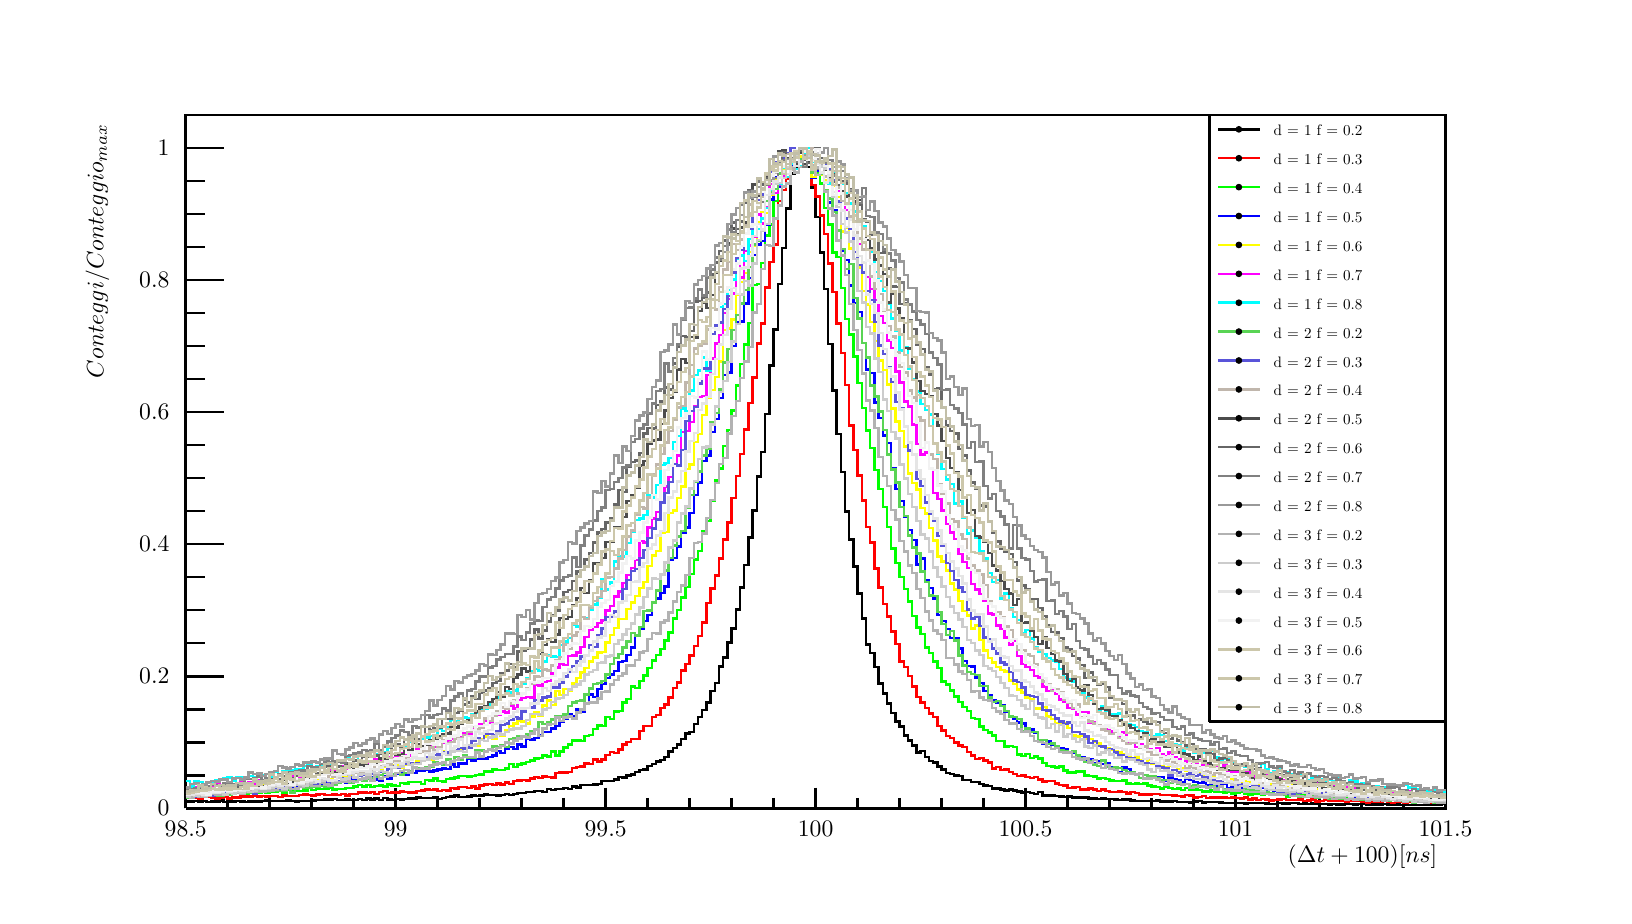
\begin{tikzpicture}
\pgfdeclareplotmark{cross} {
\pgfpathmoveto{\pgfpoint{-0.3\pgfplotmarksize}{\pgfplotmarksize}}
\pgfpathlineto{\pgfpoint{+0.3\pgfplotmarksize}{\pgfplotmarksize}}
\pgfpathlineto{\pgfpoint{+0.3\pgfplotmarksize}{0.3\pgfplotmarksize}}
\pgfpathlineto{\pgfpoint{+1\pgfplotmarksize}{0.3\pgfplotmarksize}}
\pgfpathlineto{\pgfpoint{+1\pgfplotmarksize}{-0.3\pgfplotmarksize}}
\pgfpathlineto{\pgfpoint{+0.3\pgfplotmarksize}{-0.3\pgfplotmarksize}}
\pgfpathlineto{\pgfpoint{+0.3\pgfplotmarksize}{-1.\pgfplotmarksize}}
\pgfpathlineto{\pgfpoint{-0.3\pgfplotmarksize}{-1.\pgfplotmarksize}}
\pgfpathlineto{\pgfpoint{-0.3\pgfplotmarksize}{-0.3\pgfplotmarksize}}
\pgfpathlineto{\pgfpoint{-1.\pgfplotmarksize}{-0.3\pgfplotmarksize}}
\pgfpathlineto{\pgfpoint{-1.\pgfplotmarksize}{0.3\pgfplotmarksize}}
\pgfpathlineto{\pgfpoint{-0.3\pgfplotmarksize}{0.3\pgfplotmarksize}}
\pgfpathclose
\pgfusepathqstroke
}
\pgfdeclareplotmark{cross*} {
\pgfpathmoveto{\pgfpoint{-0.3\pgfplotmarksize}{\pgfplotmarksize}}
\pgfpathlineto{\pgfpoint{+0.3\pgfplotmarksize}{\pgfplotmarksize}}
\pgfpathlineto{\pgfpoint{+0.3\pgfplotmarksize}{0.3\pgfplotmarksize}}
\pgfpathlineto{\pgfpoint{+1\pgfplotmarksize}{0.3\pgfplotmarksize}}
\pgfpathlineto{\pgfpoint{+1\pgfplotmarksize}{-0.3\pgfplotmarksize}}
\pgfpathlineto{\pgfpoint{+0.3\pgfplotmarksize}{-0.3\pgfplotmarksize}}
\pgfpathlineto{\pgfpoint{+0.3\pgfplotmarksize}{-1.\pgfplotmarksize}}
\pgfpathlineto{\pgfpoint{-0.3\pgfplotmarksize}{-1.\pgfplotmarksize}}
\pgfpathlineto{\pgfpoint{-0.3\pgfplotmarksize}{-0.3\pgfplotmarksize}}
\pgfpathlineto{\pgfpoint{-1.\pgfplotmarksize}{-0.3\pgfplotmarksize}}
\pgfpathlineto{\pgfpoint{-1.\pgfplotmarksize}{0.3\pgfplotmarksize}}
\pgfpathlineto{\pgfpoint{-0.3\pgfplotmarksize}{0.3\pgfplotmarksize}}
\pgfpathclose
\pgfusepathqfillstroke
}
\pgfdeclareplotmark{newstar} {
\pgfpathmoveto{\pgfqpoint{0pt}{\pgfplotmarksize}}
\pgfpathlineto{\pgfqpointpolar{44}{0.5\pgfplotmarksize}}
\pgfpathlineto{\pgfqpointpolar{18}{\pgfplotmarksize}}
\pgfpathlineto{\pgfqpointpolar{-20}{0.5\pgfplotmarksize}}
\pgfpathlineto{\pgfqpointpolar{-54}{\pgfplotmarksize}}
\pgfpathlineto{\pgfqpointpolar{-90}{0.5\pgfplotmarksize}}
\pgfpathlineto{\pgfqpointpolar{234}{\pgfplotmarksize}}
\pgfpathlineto{\pgfqpointpolar{198}{0.5\pgfplotmarksize}}
\pgfpathlineto{\pgfqpointpolar{162}{\pgfplotmarksize}}
\pgfpathlineto{\pgfqpointpolar{134}{0.5\pgfplotmarksize}}
\pgfpathclose
\pgfusepathqstroke
}
\pgfdeclareplotmark{newstar*} {
\pgfpathmoveto{\pgfqpoint{0pt}{\pgfplotmarksize}}
\pgfpathlineto{\pgfqpointpolar{44}{0.5\pgfplotmarksize}}
\pgfpathlineto{\pgfqpointpolar{18}{\pgfplotmarksize}}
\pgfpathlineto{\pgfqpointpolar{-20}{0.5\pgfplotmarksize}}
\pgfpathlineto{\pgfqpointpolar{-54}{\pgfplotmarksize}}
\pgfpathlineto{\pgfqpointpolar{-90}{0.5\pgfplotmarksize}}
\pgfpathlineto{\pgfqpointpolar{234}{\pgfplotmarksize}}
\pgfpathlineto{\pgfqpointpolar{198}{0.5\pgfplotmarksize}}
\pgfpathlineto{\pgfqpointpolar{162}{\pgfplotmarksize}}
\pgfpathlineto{\pgfqpointpolar{134}{0.5\pgfplotmarksize}}
\pgfpathclose
\pgfusepathqfillstroke
}
\definecolor{c}{rgb}{1,1,1};
\draw [color=c, fill=c] (0,0) rectangle (20,11.0085);
\draw [color=c, fill=c] (2,1.10085) rectangle (18,9.90762);
\definecolor{c}{rgb}{0,0,0};
\draw [c,line width=0.9] (2,1.10085) -- (2,9.90762) -- (18,9.90762) -- (18,1.10085) -- (2,1.10085);
\definecolor{c}{rgb}{1,1,1};
\draw [color=c, fill=c] (2,1.10085) rectangle (18,9.90762);
\definecolor{c}{rgb}{0,0,0};
\draw [c,line width=0.9] (2,1.10085) -- (2,9.90762) -- (18,9.90762) -- (18,1.10085) -- (2,1.10085);
\draw [c,line width=0.9] (2,1.19075) -- (2.05333,1.19075) -- (2.05333,1.19075) -- (2.10667,1.19075) -- (2.10667,1.19653) -- (2.16,1.19653) -- (2.16,1.18658) -- (2.21333,1.18658) -- (2.21333,1.19525) -- (2.26667,1.19525) -- (2.26667,1.18465) --
 (2.32,1.18465) -- (2.32,1.18947) -- (2.37333,1.18947) -- (2.37333,1.18562) -- (2.42667,1.18562) -- (2.42667,1.19782) -- (2.48,1.19782) -- (2.48,1.18401) -- (2.53333,1.18401) -- (2.53333,1.18754) -- (2.58667,1.18754) -- (2.58667,1.18722) --
 (2.64,1.18722) -- (2.64,1.19525) -- (2.69333,1.19525) -- (2.69333,1.19075) -- (2.74667,1.19075) -- (2.74667,1.1808) -- (2.8,1.1808) -- (2.8,1.18786) -- (2.85333,1.18786) -- (2.85333,1.18819) -- (2.90667,1.18819) -- (2.90667,1.18722) --
 (2.96,1.18722) -- (2.96,1.19718) -- (3.01333,1.19718) -- (3.01333,1.19782) -- (3.06667,1.19782) -- (3.06667,1.19429) -- (3.12,1.19429) -- (3.12,1.19461) -- (3.17333,1.19461) -- (3.17333,1.19364) -- (3.22667,1.19364) -- (3.22667,1.19461) --
 (3.28,1.19461) -- (3.28,1.19975) -- (3.33333,1.19975) -- (3.33333,1.19397) -- (3.38667,1.19397) -- (3.38667,1.18915) -- (3.44,1.18915) -- (3.44,1.19236) -- (3.49333,1.19236) -- (3.49333,1.19621) -- (3.54667,1.19621) -- (3.54667,1.19397) --
 (3.6,1.19397) -- (3.6,1.20296) -- (3.65333,1.20296) -- (3.65333,1.20874) -- (3.70667,1.20874) -- (3.70667,1.20585) -- (3.76,1.20585) -- (3.76,1.21163) -- (3.81333,1.21163) -- (3.81333,1.21516) -- (3.86667,1.21516) -- (3.86667,1.21644) --
 (3.92,1.21644) -- (3.92,1.20809) -- (3.97333,1.20809) -- (3.97333,1.20424) -- (4.02667,1.20424) -- (4.02667,1.21034) -- (4.08,1.21034) -- (4.08,1.20617) -- (4.13333,1.20617) -- (4.13333,1.20713) -- (4.18667,1.20713) -- (4.18667,1.21965) --
 (4.24,1.21965) -- (4.24,1.20392) -- (4.29333,1.20392) -- (4.29333,1.22319) -- (4.34667,1.22319) -- (4.34667,1.21195) -- (4.4,1.21195) -- (4.4,1.22319) -- (4.45333,1.22319) -- (4.45333,1.2052) -- (4.50667,1.2052) -- (4.50667,1.22993) --
 (4.56,1.22993) -- (4.56,1.21355) -- (4.61333,1.21355) -- (4.61333,1.2097) -- (4.66667,1.2097) -- (4.66667,1.22222) -- (4.72,1.22222) -- (4.72,1.2158) -- (4.77333,1.2158) -- (4.77333,1.21965) -- (4.82667,1.21965) -- (4.82667,1.22896) --
 (4.88,1.22896) -- (4.88,1.22704) -- (4.93333,1.22704) -- (4.93333,1.23796) -- (4.98667,1.23796) -- (4.98667,1.23346) -- (5.04,1.23346) -- (5.04,1.23057) -- (5.09333,1.23057) -- (5.09333,1.23507) -- (5.14667,1.23507) -- (5.14667,1.23635) --
 (5.2,1.23635) -- (5.2,1.21644) -- (5.25333,1.21644) -- (5.25333,1.23282) -- (5.30667,1.23282) -- (5.30667,1.24759) -- (5.36,1.24759) -- (5.36,1.24855) -- (5.41333,1.24855) -- (5.41333,1.26685) -- (5.46667,1.26685) -- (5.46667,1.2447) --
 (5.52,1.2447) -- (5.52,1.24309) -- (5.57333,1.24309) -- (5.57333,1.25273) -- (5.62667,1.25273) -- (5.62667,1.26236) -- (5.68,1.26236) -- (5.68,1.25722) -- (5.73333,1.25722) -- (5.73333,1.263) -- (5.78667,1.263) -- (5.78667,1.27392) -- (5.84,1.27392)
 -- (5.84,1.26814) -- (5.89333,1.26814) -- (5.89333,1.27039) -- (5.94667,1.27039) -- (5.94667,1.26589) -- (6,1.26589) -- (6,1.27328) -- (6.05333,1.27328) -- (6.05333,1.28612) -- (6.10667,1.28612) -- (6.10667,1.26878) -- (6.16,1.26878) --
 (6.16,1.28259) -- (6.21333,1.28259) -- (6.21333,1.29286) -- (6.26667,1.29286) -- (6.26667,1.29479) -- (6.32,1.29479) -- (6.32,1.30539) -- (6.37333,1.30539) -- (6.37333,1.30603) -- (6.42667,1.30603) -- (6.42667,1.32048) -- (6.48,1.32048) --
 (6.48,1.32048) -- (6.53333,1.32048) -- (6.53333,1.30731) -- (6.58667,1.30731) -- (6.58667,1.34649) -- (6.64,1.34649) -- (6.64,1.33107) -- (6.69333,1.33107) -- (6.69333,1.3436) -- (6.74667,1.3436) -- (6.74667,1.34906) -- (6.8,1.34906) --
 (6.8,1.36029) -- (6.85333,1.36029) -- (6.85333,1.34777) -- (6.90667,1.34777) -- (6.90667,1.37763) -- (6.96,1.37763) -- (6.96,1.36768) -- (7.01333,1.36768) -- (7.01333,1.39818) -- (7.06667,1.39818) -- (7.06667,1.39561) -- (7.12,1.39561) --
 (7.12,1.39947) -- (7.17333,1.39947) -- (7.17333,1.40461) -- (7.22667,1.40461) -- (7.22667,1.41263) -- (7.28,1.41263) -- (7.28,1.44924) -- (7.33333,1.44924) -- (7.33333,1.4486) -- (7.38667,1.4486) -- (7.38667,1.44827) -- (7.44,1.44827) --
 (7.44,1.47043) -- (7.49333,1.47043) -- (7.49333,1.49997) -- (7.54667,1.49997) -- (7.54667,1.49355) -- (7.6,1.49355) -- (7.6,1.51506) -- (7.65333,1.51506) -- (7.65333,1.52823) -- (7.70667,1.52823) -- (7.70667,1.56066) -- (7.76,1.56066) --
 (7.76,1.58667) -- (7.81333,1.58667) -- (7.81333,1.59502) -- (7.86667,1.59502) -- (7.86667,1.64061) -- (7.92,1.64061) -- (7.92,1.66566) -- (7.97333,1.66566) -- (7.97333,1.69295) -- (8.02667,1.69295) -- (8.02667,1.71703) -- (8.08,1.71703) --
 (8.08,1.75428) -- (8.13333,1.75428) -- (8.13333,1.82364) -- (8.18667,1.82364) -- (8.18667,1.86442) -- (8.24,1.86442) -- (8.24,1.91258) -- (8.29333,1.91258) -- (8.29333,1.97969) -- (8.34667,1.97969) -- (8.34667,2.05066) -- (8.4,2.05066) --
 (8.4,2.06735) -- (8.45333,2.06735) -- (8.45333,2.17364) -- (8.50667,2.17364) -- (8.50667,2.26419) -- (8.56,2.26419) -- (8.56,2.35024) -- (8.61333,2.35024) -- (8.61333,2.44239) -- (8.66667,2.44239) -- (8.66667,2.58849) -- (8.72,2.58849) --
 (8.72,2.69542) -- (8.77333,2.69542) -- (8.77333,2.90189) -- (8.82667,2.90189) -- (8.82667,3.01523) -- (8.88,3.01523) -- (8.88,3.20982) -- (8.93333,3.20982) -- (8.93333,3.3845) -- (8.98667,3.3845) -- (8.98667,3.62564) -- (9.04,3.62564) --
 (9.04,3.90468) -- (9.09333,3.90468) -- (9.09333,4.19142) -- (9.14667,4.19142) -- (9.14667,4.53949) -- (9.2,4.53949) -- (9.2,4.88274) -- (9.25333,4.88274) -- (9.25333,5.3143) -- (9.30667,5.3143) -- (9.30667,5.62897) -- (9.36,5.62897) --
 (9.36,6.11126) -- (9.41333,6.11126) -- (9.41333,6.72745) -- (9.46667,6.72745) -- (9.46667,7.18245) -- (9.52,7.18245) -- (9.52,7.76042) -- (9.57333,7.76042) -- (9.57333,8.21799) -- (9.62667,8.21799) -- (9.62667,8.71954) -- (9.68,8.71954) --
 (9.68,9.16523) -- (9.73333,9.16523) -- (9.73333,9.22463) -- (9.78667,9.22463) -- (9.78667,9.45454) -- (9.84,9.45454) -- (9.84,9.48825) -- (9.89333,9.48825) -- (9.89333,9.24357) -- (9.94667,9.24357) -- (9.94667,8.98413) -- (10,8.98413) --
 (10,8.60876) -- (10.0533,8.60876) -- (10.0533,8.16308) -- (10.1067,8.16308) -- (10.1067,7.69684) -- (10.16,7.69684) -- (10.16,6.99492) -- (10.2133,6.99492) -- (10.2133,6.40956) -- (10.2667,6.40956) -- (10.2667,5.85727) -- (10.32,5.85727) --
 (10.32,5.37145) -- (10.3733,5.37145) -- (10.3733,4.87343) -- (10.4267,4.87343) -- (10.4267,4.51476) -- (10.48,4.51476) -- (10.48,4.16958) -- (10.5333,4.16958) -- (10.5333,3.82729) -- (10.5867,3.82729) -- (10.5867,3.51486) -- (10.64,3.51486) --
 (10.64,3.18381) -- (10.6933,3.18381) -- (10.6933,3.07592) -- (10.7467,3.07592) -- (10.7467,2.89418) -- (10.8,2.89418) -- (10.8,2.68514) -- (10.8533,2.68514) -- (10.8533,2.56088) -- (10.9067,2.56088) -- (10.9067,2.43437) -- (10.96,2.43437) --
 (10.96,2.31074) -- (11.0133,2.31074) -- (11.0133,2.20607) -- (11.0667,2.20607) -- (11.0667,2.14056) -- (11.12,2.14056) -- (11.12,2.02432) -- (11.1733,2.02432) -- (11.1733,1.96492) -- (11.2267,1.96492) -- (11.2267,1.90134) -- (11.28,1.90134) --
 (11.28,1.81304) -- (11.3333,1.81304) -- (11.3333,1.83167) -- (11.3867,1.83167) -- (11.3867,1.75139) -- (11.44,1.75139) -- (11.44,1.70002) -- (11.4933,1.70002) -- (11.4933,1.68075) -- (11.5467,1.68075) -- (11.5467,1.6313) -- (11.6,1.6313) --
 (11.6,1.59148) -- (11.6533,1.59148) -- (11.6533,1.54717) -- (11.7067,1.54717) -- (11.7067,1.53818) -- (11.76,1.53818) -- (11.76,1.51538) -- (11.8133,1.51538) -- (11.8133,1.51057) -- (11.8667,1.51057) -- (11.8667,1.46176) -- (11.92,1.46176) --
 (11.92,1.45823) -- (11.9733,1.45823) -- (11.9733,1.43672) -- (12.0267,1.43672) -- (12.0267,1.43318) -- (12.08,1.43318) -- (12.08,1.41167) -- (12.1333,1.41167) -- (12.1333,1.38855) -- (12.1867,1.38855) -- (12.1867,1.38502) -- (12.24,1.38502) --
 (12.24,1.35612) -- (12.2933,1.35612) -- (12.2933,1.35612) -- (12.3467,1.35612) -- (12.3467,1.33878) -- (12.4,1.33878) -- (12.4,1.33011) -- (12.4533,1.33011) -- (12.4533,1.34135) -- (12.5067,1.34135) -- (12.5067,1.32979) -- (12.56,1.32979) --
 (12.56,1.31341) -- (12.6133,1.31341) -- (12.6133,1.30057) -- (12.6667,1.30057) -- (12.6667,1.30731) -- (12.72,1.30731) -- (12.72,1.29832) -- (12.7733,1.29832) -- (12.7733,1.28291) -- (12.8267,1.28291) -- (12.8267,1.30603) -- (12.88,1.30603) --
 (12.88,1.26525) -- (12.9333,1.26525) -- (12.9333,1.26364) -- (12.9867,1.26364) -- (12.9867,1.26621) -- (13.04,1.26621) -- (13.04,1.26011) -- (13.0933,1.26011) -- (13.0933,1.25305) -- (13.1467,1.25305) -- (13.1467,1.24727) -- (13.2,1.24727) --
 (13.2,1.25305) -- (13.2533,1.25305) -- (13.2533,1.23892) -- (13.3067,1.23892) -- (13.3067,1.24181) -- (13.36,1.24181) -- (13.36,1.23571) -- (13.4133,1.23571) -- (13.4133,1.23635) -- (13.4667,1.23635) -- (13.4667,1.22736) -- (13.52,1.22736) --
 (13.52,1.22864) -- (13.5733,1.22864) -- (13.5733,1.22062) -- (13.6267,1.22062) -- (13.6267,1.22864) -- (13.68,1.22864) -- (13.68,1.21644) -- (13.7333,1.21644) -- (13.7333,1.21708) -- (13.7867,1.21708) -- (13.7867,1.2113) -- (13.84,1.2113) --
 (13.84,1.20777) -- (13.8933,1.20777) -- (13.8933,1.21259) -- (13.9467,1.21259) -- (13.9467,1.2113) -- (14,1.2113) -- (14,1.1991) -- (14.0533,1.1991) -- (14.0533,1.19397) -- (14.1067,1.19397) -- (14.1067,1.193) -- (14.16,1.193) -- (14.16,1.19653) --
 (14.2133,1.19653) -- (14.2133,1.19429) -- (14.2667,1.19429) -- (14.2667,1.19686) -- (14.32,1.19686) -- (14.32,1.20007) -- (14.3733,1.20007) -- (14.3733,1.18497) -- (14.4267,1.18497) -- (14.4267,1.18722) -- (14.48,1.18722) -- (14.48,1.19043) --
 (14.5333,1.19043) -- (14.5333,1.19236) -- (14.5867,1.19236) -- (14.5867,1.18112) -- (14.64,1.18112) -- (14.64,1.18401) -- (14.6933,1.18401) -- (14.6933,1.18208) -- (14.7467,1.18208) -- (14.7467,1.17695) -- (14.8,1.17695) -- (14.8,1.18626) --
 (14.8533,1.18626) -- (14.8533,1.19204) -- (14.9067,1.19204) -- (14.9067,1.17534) -- (14.96,1.17534) -- (14.96,1.17855) -- (15.0133,1.17855) -- (15.0133,1.18112) -- (15.0667,1.18112) -- (15.0667,1.17887) -- (15.12,1.17887) -- (15.12,1.17727) --
 (15.1733,1.17727) -- (15.1733,1.16828) -- (15.2267,1.16828) -- (15.2267,1.17085) -- (15.28,1.17085) -- (15.28,1.16667) -- (15.3333,1.16667) -- (15.3333,1.16924) -- (15.3867,1.16924) -- (15.3867,1.16635) -- (15.44,1.16635) -- (15.44,1.16314) --
 (15.4933,1.16314) -- (15.4933,1.17181) -- (15.5467,1.17181) -- (15.5467,1.16956) -- (15.6,1.16956) -- (15.6,1.16796) -- (15.6533,1.16796) -- (15.6533,1.16796) -- (15.7067,1.16796) -- (15.7067,1.16282) -- (15.76,1.16282) -- (15.76,1.15736) --
 (15.8133,1.15736) -- (15.8133,1.15864) -- (15.8667,1.15864) -- (15.8667,1.16603) -- (15.92,1.16603) -- (15.92,1.16153) -- (15.9733,1.16153) -- (15.9733,1.16153) -- (16.0267,1.16153) -- (16.0267,1.16667) -- (16.08,1.16667) -- (16.08,1.16667) --
 (16.1333,1.16667) -- (16.1333,1.15351) -- (16.1867,1.15351) -- (16.1867,1.16314) -- (16.24,1.16314) -- (16.24,1.15575) -- (16.2933,1.15575) -- (16.2933,1.16378) -- (16.3467,1.16378) -- (16.3467,1.15575) -- (16.4,1.15575) -- (16.4,1.15929) --
 (16.4533,1.15929) -- (16.4533,1.15768) -- (16.5067,1.15768) -- (16.5067,1.14837) -- (16.56,1.14837) -- (16.56,1.15864) -- (16.6133,1.15864) -- (16.6133,1.14997) -- (16.6667,1.14997) -- (16.6667,1.14869) -- (16.72,1.14869) -- (16.72,1.15319) --
 (16.7733,1.15319) -- (16.7733,1.15319) -- (16.8267,1.15319) -- (16.8267,1.15254) -- (16.88,1.15254) -- (16.88,1.15575) -- (16.9333,1.15575) -- (16.9333,1.15319) -- (16.9867,1.15319) -- (16.9867,1.14676) -- (17.04,1.14676) -- (17.04,1.14741) --
 (17.0933,1.14741) -- (17.0933,1.15254) -- (17.1467,1.15254) -- (17.1467,1.15126) -- (17.2,1.15126) -- (17.2,1.15543) -- (17.2533,1.15543) -- (17.2533,1.14837) -- (17.3067,1.14837) -- (17.3067,1.14933) -- (17.36,1.14933) -- (17.36,1.14741) --
 (17.4133,1.14741) -- (17.4133,1.14355) -- (17.4667,1.14355) -- (17.4667,1.15158) -- (17.52,1.15158) -- (17.52,1.14195) -- (17.5733,1.14195) -- (17.5733,1.14741) -- (17.6267,1.14741) -- (17.6267,1.14644) -- (17.68,1.14644) -- (17.68,1.1442) --
 (17.7333,1.1442) -- (17.7333,1.14227) -- (17.7867,1.14227) -- (17.7867,1.14933) -- (17.84,1.14933) -- (17.84,1.1442) -- (17.8933,1.1442) -- (17.8933,1.14548) -- (17.9467,1.14548) -- (17.9467,1.15447) -- (18,1.15447);
\draw [c,line width=0.9] (2,1.10085) -- (18,1.10085);
\draw [anchor= east] (18,0.484373) node[scale=0.854877, color=c, rotate=0]{$(\Delta t + 100) [ns]$};
\draw [c,line width=0.9] (2,1.36505) -- (2,1.10085);
\draw [c,line width=0.9] (2.53333,1.23295) -- (2.53333,1.10085);
\draw [c,line width=0.9] (3.06667,1.23295) -- (3.06667,1.10085);
\draw [c,line width=0.9] (3.6,1.23295) -- (3.6,1.10085);
\draw [c,line width=0.9] (4.13333,1.23295) -- (4.13333,1.10085);
\draw [c,line width=0.9] (4.66667,1.36505) -- (4.66667,1.10085);
\draw [c,line width=0.9] (5.2,1.23295) -- (5.2,1.10085);
\draw [c,line width=0.9] (5.73333,1.23295) -- (5.73333,1.10085);
\draw [c,line width=0.9] (6.26667,1.23295) -- (6.26667,1.10085);
\draw [c,line width=0.9] (6.8,1.23295) -- (6.8,1.10085);
\draw [c,line width=0.9] (7.33333,1.36505) -- (7.33333,1.10085);
\draw [c,line width=0.9] (7.86667,1.23295) -- (7.86667,1.10085);
\draw [c,line width=0.9] (8.4,1.23295) -- (8.4,1.10085);
\draw [c,line width=0.9] (8.93333,1.23295) -- (8.93333,1.10085);
\draw [c,line width=0.9] (9.46667,1.23295) -- (9.46667,1.10085);
\draw [c,line width=0.9] (10,1.36505) -- (10,1.10085);
\draw [c,line width=0.9] (10.5333,1.23295) -- (10.5333,1.10085);
\draw [c,line width=0.9] (11.0667,1.23295) -- (11.0667,1.10085);
\draw [c,line width=0.9] (11.6,1.23295) -- (11.6,1.10085);
\draw [c,line width=0.9] (12.1333,1.23295) -- (12.1333,1.10085);
\draw [c,line width=0.9] (12.6667,1.36505) -- (12.6667,1.10085);
\draw [c,line width=0.9] (13.2,1.23295) -- (13.2,1.10085);
\draw [c,line width=0.9] (13.7333,1.23295) -- (13.7333,1.10085);
\draw [c,line width=0.9] (14.2667,1.23295) -- (14.2667,1.10085);
\draw [c,line width=0.9] (14.8,1.23295) -- (14.8,1.10085);
\draw [c,line width=0.9] (15.3333,1.36505) -- (15.3333,1.10085);
\draw [c,line width=0.9] (15.8667,1.23295) -- (15.8667,1.10085);
\draw [c,line width=0.9] (16.4,1.23295) -- (16.4,1.10085);
\draw [c,line width=0.9] (16.9333,1.23295) -- (16.9333,1.10085);
\draw [c,line width=0.9] (17.4667,1.23295) -- (17.4667,1.10085);
\draw [c,line width=0.9] (18,1.36505) -- (18,1.10085);
\draw [c,line width=0.9] (18,1.36505) -- (18,1.10085);
\draw [anchor=base] (2,0.737567) node[scale=0.854877, color=c, rotate=0]{98.5};
\draw [anchor=base] (4.66667,0.737567) node[scale=0.854877, color=c, rotate=0]{99};
\draw [anchor=base] (7.33333,0.737567) node[scale=0.854877, color=c, rotate=0]{99.5};
\draw [anchor=base] (10,0.737567) node[scale=0.854877, color=c, rotate=0]{100};
\draw [anchor=base] (12.6667,0.737567) node[scale=0.854877, color=c, rotate=0]{100.5};
\draw [anchor=base] (15.3333,0.737567) node[scale=0.854877, color=c, rotate=0]{101};
\draw [anchor=base] (18,0.737567) node[scale=0.854877, color=c, rotate=0]{101.5};
\draw [c,line width=0.9] (2,1.10085) -- (2,9.90762);
\draw [anchor= east] (0.88,9.90762) node[scale=0.854877, color=c, rotate=90]{$Conteggi/Conteggio_{max}$};
\draw [c,line width=0.9] (2.48,1.10085) -- (2,1.10085);
\draw [c,line width=0.9] (2.24,1.52022) -- (2,1.52022);
\draw [c,line width=0.9] (2.24,1.93959) -- (2,1.93959);
\draw [c,line width=0.9] (2.24,2.35896) -- (2,2.35896);
\draw [c,line width=0.9] (2.48,2.77833) -- (2,2.77833);
\draw [c,line width=0.9] (2.24,3.1977) -- (2,3.1977);
\draw [c,line width=0.9] (2.24,3.61707) -- (2,3.61707);
\draw [c,line width=0.9] (2.24,4.03644) -- (2,4.03644);
\draw [c,line width=0.9] (2.48,4.45581) -- (2,4.45581);
\draw [c,line width=0.9] (2.24,4.87518) -- (2,4.87518);
\draw [c,line width=0.9] (2.24,5.29455) -- (2,5.29455);
\draw [c,line width=0.9] (2.24,5.71392) -- (2,5.71392);
\draw [c,line width=0.9] (2.48,6.13329) -- (2,6.13329);
\draw [c,line width=0.9] (2.24,6.55266) -- (2,6.55266);
\draw [c,line width=0.9] (2.24,6.97203) -- (2,6.97203);
\draw [c,line width=0.9] (2.24,7.3914) -- (2,7.3914);
\draw [c,line width=0.9] (2.48,7.81077) -- (2,7.81077);
\draw [c,line width=0.9] (2.24,8.23014) -- (2,8.23014);
\draw [c,line width=0.9] (2.24,8.64951) -- (2,8.64951);
\draw [c,line width=0.9] (2.24,9.06888) -- (2,9.06888);
\draw [c,line width=0.9] (2.48,9.48825) -- (2,9.48825);
\draw [c,line width=0.9] (2.48,9.48825) -- (2,9.48825);
\draw [anchor= east] (1.9,1.10085) node[scale=0.854877, color=c, rotate=0]{0};
\draw [anchor= east] (1.9,2.77833) node[scale=0.854877, color=c, rotate=0]{0.2};
\draw [anchor= east] (1.9,4.45581) node[scale=0.854877, color=c, rotate=0]{0.4};
\draw [anchor= east] (1.9,6.13329) node[scale=0.854877, color=c, rotate=0]{0.6};
\draw [anchor= east] (1.9,7.81077) node[scale=0.854877, color=c, rotate=0]{0.8};
\draw [anchor= east] (1.9,9.48825) node[scale=0.854877, color=c, rotate=0]{1};
\definecolor{c}{rgb}{1,0,0};
\draw [c,line width=0.9] (2,1.23603) -- (2.05333,1.23603) -- (2.05333,1.23116) -- (2.10667,1.23116) -- (2.10667,1.23869) -- (2.16,1.23869) -- (2.16,1.22584) -- (2.21333,1.22584) -- (2.21333,1.24579) -- (2.26667,1.24579) -- (2.26667,1.24534) --
 (2.32,1.24534) -- (2.32,1.23648) -- (2.37333,1.23648) -- (2.37333,1.2285) -- (2.42667,1.2285) -- (2.42667,1.23692) -- (2.48,1.23692) -- (2.48,1.24712) -- (2.53333,1.24712) -- (2.53333,1.22894) -- (2.58667,1.22894) -- (2.58667,1.23914) --
 (2.64,1.23914) -- (2.64,1.24091) -- (2.69333,1.24091) -- (2.69333,1.25332) -- (2.74667,1.25332) -- (2.74667,1.2511) -- (2.8,1.2511) -- (2.8,1.25155) -- (2.85333,1.25155) -- (2.85333,1.2582) -- (2.90667,1.2582) -- (2.90667,1.25066) -- (2.96,1.25066)
 -- (2.96,1.25731) -- (3.01333,1.25731) -- (3.01333,1.24933) -- (3.06667,1.24933) -- (3.06667,1.25775) -- (3.12,1.25775) -- (3.12,1.25642) -- (3.17333,1.25642) -- (3.17333,1.24534) -- (3.22667,1.24534) -- (3.22667,1.26352) -- (3.28,1.26352) --
 (3.28,1.25465) -- (3.33333,1.25465) -- (3.33333,1.26041) -- (3.38667,1.26041) -- (3.38667,1.25864) -- (3.44,1.25864) -- (3.44,1.2675) -- (3.49333,1.2675) -- (3.49333,1.27814) -- (3.54667,1.27814) -- (3.54667,1.26883) -- (3.6,1.26883) --
 (3.6,1.26529) -- (3.65333,1.26529) -- (3.65333,1.2777) -- (3.70667,1.2777) -- (3.70667,1.2808) -- (3.76,1.2808) -- (3.76,1.26972) -- (3.81333,1.26972) -- (3.81333,1.27194) -- (3.86667,1.27194) -- (3.86667,1.27903) -- (3.92,1.27903) -- (3.92,1.26883)
 -- (3.97333,1.26883) -- (3.97333,1.28346) -- (4.02667,1.28346) -- (4.02667,1.26396) -- (4.08,1.26396) -- (4.08,1.28612) -- (4.13333,1.28612) -- (4.13333,1.28213) -- (4.18667,1.28213) -- (4.18667,1.29942) -- (4.24,1.29942) -- (4.24,1.30341) --
 (4.29333,1.30341) -- (4.29333,1.29587) -- (4.34667,1.29587) -- (4.34667,1.30828) -- (4.4,1.30828) -- (4.4,1.28036) -- (4.45333,1.28036) -- (4.45333,1.30873) -- (4.50667,1.30873) -- (4.50667,1.32025) -- (4.56,1.32025) -- (4.56,1.29809) --
 (4.61333,1.29809) -- (4.61333,1.3003) -- (4.66667,1.3003) -- (4.66667,1.30429) -- (4.72,1.30429) -- (4.72,1.3167) -- (4.77333,1.3167) -- (4.77333,1.31139) -- (4.82667,1.31139) -- (4.82667,1.30474) -- (4.88,1.30474) -- (4.88,1.3003) --
 (4.93333,1.3003) -- (4.93333,1.32158) -- (4.98667,1.32158) -- (4.98667,1.32911) -- (5.04,1.32911) -- (5.04,1.33754) -- (5.09333,1.33754) -- (5.09333,1.33266) -- (5.14667,1.33266) -- (5.14667,1.34241) -- (5.2,1.34241) -- (5.2,1.32291) --
 (5.25333,1.32291) -- (5.25333,1.33621) -- (5.30667,1.33621) -- (5.30667,1.32911) -- (5.36,1.32911) -- (5.36,1.36236) -- (5.41333,1.36236) -- (5.41333,1.35571) -- (5.46667,1.35571) -- (5.46667,1.37122) -- (5.52,1.37122) -- (5.52,1.37388) --
 (5.57333,1.37388) -- (5.57333,1.36147) -- (5.62667,1.36147) -- (5.62667,1.37787) -- (5.68,1.37787) -- (5.68,1.35527) -- (5.73333,1.35527) -- (5.73333,1.38851) -- (5.78667,1.38851) -- (5.78667,1.40491) -- (5.84,1.40491) -- (5.84,1.41289) --
 (5.89333,1.41289) -- (5.89333,1.39915) -- (5.94667,1.39915) -- (5.94667,1.41422) -- (6,1.41422) -- (6,1.40624) -- (6.05333,1.40624) -- (6.05333,1.42973) -- (6.10667,1.42973) -- (6.10667,1.41244) -- (6.16,1.41244) -- (6.16,1.44702) --
 (6.21333,1.44702) -- (6.21333,1.45455) -- (6.26667,1.45455) -- (6.26667,1.46209) -- (6.32,1.46209) -- (6.32,1.45588) -- (6.37333,1.45588) -- (6.37333,1.48203) -- (6.42667,1.48203) -- (6.42667,1.49976) -- (6.48,1.49976) -- (6.48,1.48691) --
 (6.53333,1.48691) -- (6.53333,1.5073) -- (6.58667,1.5073) -- (6.58667,1.49622) -- (6.64,1.49622) -- (6.64,1.49533) -- (6.69333,1.49533) -- (6.69333,1.54719) -- (6.74667,1.54719) -- (6.74667,1.55916) -- (6.8,1.55916) -- (6.8,1.5565) --
 (6.85333,1.5565) -- (6.85333,1.5627) -- (6.90667,1.5627) -- (6.90667,1.61323) -- (6.96,1.61323) -- (6.96,1.62298) -- (7.01333,1.62298) -- (7.01333,1.63318) -- (7.06667,1.63318) -- (7.06667,1.67041) -- (7.12,1.67041) -- (7.12,1.66598) --
 (7.17333,1.66598) -- (7.17333,1.72271) -- (7.22667,1.72271) -- (7.22667,1.69479) -- (7.28,1.69479) -- (7.28,1.72182) -- (7.33333,1.72182) -- (7.33333,1.77856) -- (7.38667,1.77856) -- (7.38667,1.81934) -- (7.44,1.81934) -- (7.44,1.80693) --
 (7.49333,1.80693) -- (7.49333,1.85081) -- (7.54667,1.85081) -- (7.54667,1.90976) -- (7.6,1.90976) -- (7.6,1.94389) -- (7.65333,1.94389) -- (7.65333,1.98201) -- (7.70667,1.98201) -- (7.70667,1.97935) -- (7.76,1.97935) -- (7.76,2.08262) --
 (7.81333,2.08262) -- (7.81333,2.146) -- (7.86667,2.146) -- (7.86667,2.146) -- (7.92,2.146) -- (7.92,2.25814) -- (7.97333,2.25814) -- (7.97333,2.28651) -- (8.02667,2.28651) -- (8.02667,2.37427) -- (8.08,2.37427) -- (8.08,2.41992) -- (8.13333,2.41992)
 -- (8.13333,2.51123) -- (8.18667,2.51123) -- (8.18667,2.6278) -- (8.24,2.6278) -- (8.24,2.69739) -- (8.29333,2.69739) -- (8.29333,2.85208) -- (8.34667,2.85208) -- (8.34667,2.93452) -- (8.4,2.93452) -- (8.4,3.044) -- (8.45333,3.044) --
 (8.45333,3.16457) -- (8.50667,3.16457) -- (8.50667,3.28823) -- (8.56,3.28823) -- (8.56,3.45976) -- (8.61333,3.45976) -- (8.61333,3.70709) -- (8.66667,3.70709) -- (8.66667,3.89591) -- (8.72,3.89591) -- (8.72,4.05725) -- (8.77333,4.05725) --
 (8.77333,4.27621) -- (8.82667,4.27621) -- (8.82667,4.51423) -- (8.88,4.51423) -- (8.88,4.73363) -- (8.93333,4.73363) -- (8.93333,5.04257) -- (8.98667,5.04257) -- (8.98667,5.32491) -- (9.04,5.32491) -- (9.04,5.60193) -- (9.09333,5.60193) --
 (9.09333,5.91486) -- (9.14667,5.91486) -- (9.14667,6.25084) -- (9.2,6.25084) -- (9.2,6.57218) -- (9.25333,6.57218) -- (9.25333,7.00656) -- (9.30667,7.00656) -- (9.30667,7.25787) -- (9.36,7.25787) -- (9.36,7.71485) -- (9.41333,7.71485) --
 (9.41333,8.04241) -- (9.46667,8.04241) -- (9.46667,8.25915) -- (9.52,8.25915) -- (9.52,8.81719) -- (9.57333,8.81719) -- (9.57333,8.9537) -- (9.62667,8.9537) -- (9.62667,9.09421) -- (9.68,9.09421) -- (9.68,9.39074) -- (9.73333,9.39074) --
 (9.73333,9.41778) -- (9.78667,9.41778) -- (9.78667,9.48825) -- (9.84,9.48825) -- (9.84,9.40536) -- (9.89333,9.40536) -- (9.89333,9.29987) -- (9.94667,9.29987) -- (9.94667,9.01886) -- (10,9.01886) -- (10,8.87259) -- (10.0533,8.87259) --
 (10.0533,8.63103) -- (10.1067,8.63103) -- (10.1067,8.39301) -- (10.16,8.39301) -- (10.16,8.01758) -- (10.2133,8.01758) -- (10.2133,7.65723) -- (10.2667,7.65723) -- (10.2667,7.25566) -- (10.32,7.25566) -- (10.32,6.886) -- (10.3733,6.886) --
 (10.3733,6.4791) -- (10.4267,6.4791) -- (10.4267,5.96495) -- (10.48,5.96495) -- (10.48,5.65069) -- (10.5333,5.65069) -- (10.5333,5.32757) -- (10.5867,5.32757) -- (10.5867,5.01198) -- (10.64,5.01198) -- (10.64,4.67468) -- (10.6933,4.67468) --
 (10.6933,4.47788) -- (10.7467,4.47788) -- (10.7467,4.14412) -- (10.8,4.14412) -- (10.8,3.90477) -- (10.8533,3.90477) -- (10.8533,3.69557) -- (10.9067,3.69557) -- (10.9067,3.54043) -- (10.96,3.54043) -- (10.96,3.34629) -- (11.0133,3.34629) --
 (11.0133,3.1885) -- (11.0667,3.1885) -- (11.0667,2.96334) -- (11.12,2.96334) -- (11.12,2.89685) -- (11.1733,2.89685) -- (11.1733,2.78205) -- (11.2267,2.78205) -- (11.2267,2.64997) -- (11.28,2.64997) -- (11.28,2.51744) -- (11.3333,2.51744) --
 (11.3333,2.44652) -- (11.3867,2.44652) -- (11.3867,2.37693) -- (11.44,2.37693) -- (11.44,2.30823) -- (11.4933,2.30823) -- (11.4933,2.26258) -- (11.5467,2.26258) -- (11.5467,2.14512) -- (11.6,2.14512) -- (11.6,2.09237) -- (11.6533,2.09237) --
 (11.6533,2.01746) -- (11.7067,2.01746) -- (11.7067,1.9953) -- (11.76,1.9953) -- (11.76,1.93768) -- (11.8133,1.93768) -- (11.8133,1.89956) -- (11.8667,1.89956) -- (11.8667,1.87962) -- (11.92,1.87962) -- (11.92,1.81756) -- (11.9733,1.81756) --
 (11.9733,1.77413) -- (12.0267,1.77413) -- (12.0267,1.72581) -- (12.08,1.72581) -- (12.08,1.7431) -- (12.1333,1.7431) -- (12.1333,1.70675) -- (12.1867,1.70675) -- (12.1867,1.68149) -- (12.24,1.68149) -- (12.24,1.60437) -- (12.2933,1.60437) --
 (12.2933,1.62697) -- (12.3467,1.62697) -- (12.3467,1.59063) -- (12.4,1.59063) -- (12.4,1.59727) -- (12.4533,1.59727) -- (12.4533,1.56447) -- (12.5067,1.56447) -- (12.5067,1.53832) -- (12.56,1.53832) -- (12.56,1.51173) -- (12.6133,1.51173) --
 (12.6133,1.51705) -- (12.6667,1.51705) -- (12.6667,1.49622) -- (12.72,1.49622) -- (12.72,1.48779) -- (12.7733,1.48779) -- (12.7733,1.49843) -- (12.8267,1.49843) -- (12.8267,1.46918) -- (12.88,1.46918) -- (12.88,1.44258) -- (12.9333,1.44258) --
 (12.9333,1.44657) -- (12.9867,1.44657) -- (12.9867,1.44923) -- (13.04,1.44923) -- (13.04,1.41732) -- (13.0933,1.41732) -- (13.0933,1.39516) -- (13.1467,1.39516) -- (13.1467,1.39294) -- (13.2,1.39294) -- (13.2,1.3597) -- (13.2533,1.3597) --
 (13.2533,1.36457) -- (13.3067,1.36457) -- (13.3067,1.37167) -- (13.36,1.37167) -- (13.36,1.3402) -- (13.4133,1.3402) -- (13.4133,1.34108) -- (13.4667,1.34108) -- (13.4667,1.35527) -- (13.52,1.35527) -- (13.52,1.33975) -- (13.5733,1.33975) --
 (13.5733,1.32335) -- (13.6267,1.32335) -- (13.6267,1.33754) -- (13.68,1.33754) -- (13.68,1.32069) -- (13.7333,1.32069) -- (13.7333,1.30917) -- (13.7867,1.30917) -- (13.7867,1.30784) -- (13.84,1.30784) -- (13.84,1.31582) -- (13.8933,1.31582) --
 (13.8933,1.30651) -- (13.9467,1.30651) -- (13.9467,1.29055) -- (14,1.29055) -- (14,1.30562) -- (14.0533,1.30562) -- (14.0533,1.29277) -- (14.1067,1.29277) -- (14.1067,1.27415) -- (14.16,1.27415) -- (14.16,1.27504) -- (14.2133,1.27504) --
 (14.2133,1.27859) -- (14.2667,1.27859) -- (14.2667,1.28302) -- (14.32,1.28302) -- (14.32,1.28435) -- (14.3733,1.28435) -- (14.3733,1.27194) -- (14.4267,1.27194) -- (14.4267,1.26839) -- (14.48,1.26839) -- (14.48,1.27282) -- (14.5333,1.27282) --
 (14.5333,1.26485) -- (14.5867,1.26485) -- (14.5867,1.2582) -- (14.64,1.2582) -- (14.64,1.24845) -- (14.6933,1.24845) -- (14.6933,1.27238) -- (14.7467,1.27238) -- (14.7467,1.26529) -- (14.8,1.26529) -- (14.8,1.23692) -- (14.8533,1.23692) --
 (14.8533,1.24756) -- (14.9067,1.24756) -- (14.9067,1.25908) -- (14.96,1.25908) -- (14.96,1.23559) -- (15.0133,1.23559) -- (15.0133,1.23958) -- (15.0667,1.23958) -- (15.0667,1.24047) -- (15.12,1.24047) -- (15.12,1.23692) -- (15.1733,1.23692) --
 (15.1733,1.23914) -- (15.2267,1.23914) -- (15.2267,1.23293) -- (15.28,1.23293) -- (15.28,1.23603) -- (15.3333,1.23603) -- (15.3333,1.22939) -- (15.3867,1.22939) -- (15.3867,1.22451) -- (15.44,1.22451) -- (15.44,1.23825) -- (15.4933,1.23825) --
 (15.4933,1.21565) -- (15.5467,1.21565) -- (15.5467,1.2254) -- (15.6,1.2254) -- (15.6,1.20722) -- (15.6533,1.20722) -- (15.6533,1.22141) -- (15.7067,1.22141) -- (15.7067,1.21609) -- (15.76,1.21609) -- (15.76,1.20279) -- (15.8133,1.20279) --
 (15.8133,1.20855) -- (15.8667,1.20855) -- (15.8667,1.21077) -- (15.92,1.21077) -- (15.92,1.22141) -- (15.9733,1.22141) -- (15.9733,1.20456) -- (16.0267,1.20456) -- (16.0267,1.20722) -- (16.08,1.20722) -- (16.08,1.20944) -- (16.1333,1.20944) --
 (16.1333,1.2152) -- (16.1867,1.2152) -- (16.1867,1.19614) -- (16.24,1.19614) -- (16.24,1.20191) -- (16.2933,1.20191) -- (16.2933,1.21254) -- (16.3467,1.21254) -- (16.3467,1.18905) -- (16.4,1.18905) -- (16.4,1.19703) -- (16.4533,1.19703) --
 (16.4533,1.20722) -- (16.5067,1.20722) -- (16.5067,1.19215) -- (16.56,1.19215) -- (16.56,1.20368) -- (16.6133,1.20368) -- (16.6133,1.19614) -- (16.6667,1.19614) -- (16.6667,1.20146) -- (16.72,1.20146) -- (16.72,1.19082) -- (16.7733,1.19082) --
 (16.7733,1.1926) -- (16.8267,1.1926) -- (16.8267,1.19526) -- (16.88,1.19526) -- (16.88,1.19526) -- (16.9333,1.19526) -- (16.9333,1.18196) -- (16.9867,1.18196) -- (16.9867,1.17442) -- (17.04,1.17442) -- (17.04,1.18861) -- (17.0933,1.18861) --
 (17.0933,1.18506) -- (17.1467,1.18506) -- (17.1467,1.18861) -- (17.2,1.18861) -- (17.2,1.19348) -- (17.2533,1.19348) -- (17.2533,1.1824) -- (17.3067,1.1824) -- (17.3067,1.17044) -- (17.36,1.17044) -- (17.36,1.18861) -- (17.4133,1.18861) --
 (17.4133,1.18196) -- (17.4667,1.18196) -- (17.4667,1.17575) -- (17.52,1.17575) -- (17.52,1.18373) -- (17.5733,1.18373) -- (17.5733,1.18816) -- (17.6267,1.18816) -- (17.6267,1.18462) -- (17.68,1.18462) -- (17.68,1.1824) -- (17.7333,1.1824) --
 (17.7333,1.18152) -- (17.7867,1.18152) -- (17.7867,1.17221) -- (17.84,1.17221) -- (17.84,1.17886) -- (17.8933,1.17886) -- (17.8933,1.17664) -- (17.9467,1.17664) -- (17.9467,1.17265) -- (18,1.17265);
\definecolor{c}{rgb}{0,1,0};
\draw [c,line width=0.9] (2,1.26593) -- (2.05333,1.26593) -- (2.05333,1.27377) -- (2.10667,1.27377) -- (2.10667,1.26817) -- (2.16,1.26817) -- (2.16,1.28999) -- (2.21333,1.28999) -- (2.21333,1.26537) -- (2.26667,1.26537) -- (2.26667,1.26537) --
 (2.32,1.26537) -- (2.32,1.28272) -- (2.37333,1.28272) -- (2.37333,1.29055) -- (2.42667,1.29055) -- (2.42667,1.28552) -- (2.48,1.28552) -- (2.48,1.2816) -- (2.53333,1.2816) -- (2.53333,1.3135) -- (2.58667,1.3135) -- (2.58667,1.29559) --
 (2.64,1.29559) -- (2.64,1.29335) -- (2.69333,1.29335) -- (2.69333,1.29447) -- (2.74667,1.29447) -- (2.74667,1.28552) -- (2.8,1.28552) -- (2.8,1.31182) -- (2.85333,1.31182) -- (2.85333,1.30958) -- (2.90667,1.30958) -- (2.90667,1.29447) --
 (2.96,1.29447) -- (2.96,1.32077) -- (3.01333,1.32077) -- (3.01333,1.29839) -- (3.06667,1.29839) -- (3.06667,1.31126) -- (3.12,1.31126) -- (3.12,1.30678) -- (3.17333,1.30678) -- (3.17333,1.3398) -- (3.22667,1.3398) -- (3.22667,1.3051) --
 (3.28,1.3051) -- (3.28,1.33141) -- (3.33333,1.33141) -- (3.33333,1.31294) -- (3.38667,1.31294) -- (3.38667,1.32469) -- (3.44,1.32469) -- (3.44,1.32189) -- (3.49333,1.32189) -- (3.49333,1.32861) -- (3.54667,1.32861) -- (3.54667,1.35883) --
 (3.6,1.35883) -- (3.6,1.337) -- (3.65333,1.337) -- (3.65333,1.34428) -- (3.70667,1.34428) -- (3.70667,1.34875) -- (3.76,1.34875) -- (3.76,1.34763) -- (3.81333,1.34763) -- (3.81333,1.35827) -- (3.86667,1.35827) -- (3.86667,1.33924) -- (3.92,1.33924)
 -- (3.92,1.34819) -- (3.97333,1.34819) -- (3.97333,1.34651) -- (4.02667,1.34651) -- (4.02667,1.35715) -- (4.08,1.35715) -- (4.08,1.36162) -- (4.13333,1.36162) -- (4.13333,1.37785) -- (4.18667,1.37785) -- (4.18667,1.39464) -- (4.24,1.39464) --
 (4.24,1.37841) -- (4.29333,1.37841) -- (4.29333,1.3952) -- (4.34667,1.3952) -- (4.34667,1.37282) -- (4.4,1.37282) -- (4.4,1.38737) -- (4.45333,1.38737) -- (4.45333,1.39184) -- (4.50667,1.39184) -- (4.50667,1.38065) -- (4.56,1.38065) --
 (4.56,1.40192) -- (4.61333,1.40192) -- (4.61333,1.39184) -- (4.66667,1.39184) -- (4.66667,1.38401) -- (4.72,1.38401) -- (4.72,1.42374) -- (4.77333,1.42374) -- (4.77333,1.41703) -- (4.82667,1.41703) -- (4.82667,1.43717) -- (4.88,1.43717) --
 (4.88,1.43493) -- (4.93333,1.43493) -- (4.93333,1.43493) -- (4.98667,1.43493) -- (4.98667,1.41087) -- (5.04,1.41087) -- (5.04,1.46067) -- (5.09333,1.46067) -- (5.09333,1.45396) -- (5.14667,1.45396) -- (5.14667,1.47858) -- (5.2,1.47858) --
 (5.2,1.4506) -- (5.25333,1.4506) -- (5.25333,1.44221) -- (5.30667,1.44221) -- (5.30667,1.47578) -- (5.36,1.47578) -- (5.36,1.48082) -- (5.41333,1.48082) -- (5.41333,1.49201) -- (5.46667,1.49201) -- (5.46667,1.50936) -- (5.52,1.50936) --
 (5.52,1.51104) -- (5.57333,1.51104) -- (5.57333,1.50712) -- (5.62667,1.50712) -- (5.62667,1.5144) -- (5.68,1.5144) -- (5.68,1.52671) -- (5.73333,1.52671) -- (5.73333,1.52839) -- (5.78667,1.52839) -- (5.78667,1.56812) -- (5.84,1.56812) --
 (5.84,1.56588) -- (5.89333,1.56588) -- (5.89333,1.59274) -- (5.94667,1.59274) -- (5.94667,1.58882) -- (6,1.58882) -- (6,1.58491) -- (6.05333,1.58491) -- (6.05333,1.60785) -- (6.10667,1.60785) -- (6.10667,1.66437) -- (6.16,1.66437) -- (6.16,1.6252)
 -- (6.21333,1.6252) -- (6.21333,1.66045) -- (6.26667,1.66045) -- (6.26667,1.67221) -- (6.32,1.67221) -- (6.32,1.68788) -- (6.37333,1.68788) -- (6.37333,1.7097) -- (6.42667,1.7097) -- (6.42667,1.73097) -- (6.48,1.73097) -- (6.48,1.74104) --
 (6.53333,1.74104) -- (6.53333,1.7735) -- (6.58667,1.7735) -- (6.58667,1.7623) -- (6.64,1.7623) -- (6.64,1.82162) -- (6.69333,1.82162) -- (6.69333,1.7735) -- (6.74667,1.7735) -- (6.74667,1.82218) -- (6.8,1.82218) -- (6.8,1.8759) -- (6.85333,1.8759)
 -- (6.85333,1.91396) -- (6.90667,1.91396) -- (6.90667,1.9632) -- (6.96,1.9632) -- (6.96,1.9632) -- (7.01333,1.9632) -- (7.01333,1.95649) -- (7.06667,1.95649) -- (7.06667,2.01916) -- (7.12,2.01916) -- (7.12,2.03483) -- (7.17333,2.03483) --
 (7.17333,2.10646) -- (7.22667,2.10646) -- (7.22667,2.15403) -- (7.28,2.15403) -- (7.28,2.14675) -- (7.33333,2.14675) -- (7.33333,2.26315) -- (7.38667,2.26315) -- (7.38667,2.23573) -- (7.44,2.23573) -- (7.44,2.32919) -- (7.49333,2.32919) --
 (7.49333,2.33478) -- (7.54667,2.33478) -- (7.54667,2.44279) -- (7.6,2.44279) -- (7.6,2.48644) -- (7.65333,2.48644) -- (7.65333,2.6504) -- (7.70667,2.6504) -- (7.70667,2.62914) -- (7.76,2.62914) -- (7.76,2.71699) -- (7.81333,2.71699) --
 (7.81333,2.78974) -- (7.86667,2.78974) -- (7.86667,2.88376) -- (7.92,2.88376) -- (7.92,2.97721) -- (7.97333,2.97721) -- (7.97333,3.04996) -- (8.02667,3.04996) -- (8.02667,3.12775) -- (8.08,3.12775) -- (8.08,3.23463) -- (8.13333,3.23463) --
 (8.13333,3.33704) -- (8.18667,3.33704) -- (8.18667,3.5122) -- (8.24,3.5122) -- (8.24,3.62244) -- (8.29333,3.62244) -- (8.29333,3.77913) -- (8.34667,3.77913) -- (8.34667,3.91064) -- (8.4,3.91064) -- (8.4,4.07628) -- (8.45333,4.07628) --
 (8.45333,4.25927) -- (8.50667,4.25927) -- (8.50667,4.36672) -- (8.56,4.36672) -- (8.56,4.6219) -- (8.61333,4.6219) -- (8.61333,4.75285) -- (8.66667,4.75285) -- (8.66667,5.00243) -- (8.72,5.00243) -- (8.72,5.26769) -- (8.77333,5.26769) --
 (8.77333,5.41654) -- (8.82667,5.41654) -- (8.82667,5.69971) -- (8.88,5.69971) -- (8.88,5.90732) -- (8.93333,5.90732) -- (8.93333,6.15634) -- (8.98667,6.15634) -- (8.98667,6.46973) -- (9.04,6.46973) -- (9.04,6.74729) -- (9.09333,6.74729) --
 (9.09333,6.99408) -- (9.14667,6.99408) -- (9.14667,7.26381) -- (9.2,7.26381) -- (9.2,7.74563) -- (9.25333,7.74563) -- (9.25333,7.75962) -- (9.30667,7.75962) -- (9.30667,8.026) -- (9.36,8.026) -- (9.36,8.37463) -- (9.41333,8.37463) --
 (9.41333,8.51845) -- (9.46667,8.51845) -- (9.46667,8.81336) -- (9.52,8.81336) -- (9.52,8.99244) -- (9.57333,8.99244) -- (9.57333,9.14297) -- (9.62667,9.14297) -- (9.62667,9.33436) -- (9.68,9.33436) -- (9.68,9.35506) -- (9.73333,9.35506) --
 (9.73333,9.30582) -- (9.78667,9.30582) -- (9.78667,9.48825) -- (9.84,9.48825) -- (9.84,9.33828) -- (9.89333,9.33828) -- (9.89333,9.34667) -- (9.94667,9.34667) -- (9.94667,9.20789) -- (10,9.20789) -- (10,9.18047) -- (10.0533,9.18047) --
 (10.0533,9.03497) -- (10.1067,9.03497) -- (10.1067,8.7255) -- (10.16,8.7255) -- (10.16,8.51453) -- (10.2133,8.51453) -- (10.2133,8.15974) -- (10.2667,8.15974) -- (10.2667,8.10378) -- (10.32,8.10378) -- (10.32,7.70702) -- (10.3733,7.70702) --
 (10.3733,7.31865) -- (10.4267,7.31865) -- (10.4267,7.12055) -- (10.48,7.12055) -- (10.48,6.84019) -- (10.5333,6.84019) -- (10.5333,6.50218) -- (10.5867,6.50218) -- (10.5867,6.18544) -- (10.64,6.18544) -- (10.64,5.90004) -- (10.6933,5.90004) --
 (10.6933,5.68012) -- (10.7467,5.68012) -- (10.7467,5.39808) -- (10.8,5.39808) -- (10.8,5.15353) -- (10.8533,5.15353) -- (10.8533,4.92633) -- (10.9067,4.92633) -- (10.9067,4.67394) -- (10.96,4.67394) -- (10.96,4.40197) -- (11.0133,4.40197) --
 (11.0133,4.21507) -- (11.0667,4.21507) -- (11.0667,4.03879) -- (11.12,4.03879) -- (11.12,3.88434) -- (11.1733,3.88434) -- (11.1733,3.72709) -- (11.2267,3.72709) -- (11.2267,3.54521) -- (11.28,3.54521) -- (11.28,3.39636) -- (11.3333,3.39636) --
 (11.3333,3.31578) -- (11.3867,3.31578) -- (11.3867,3.14174) -- (11.44,3.14174) -- (11.44,3.07626) -- (11.4933,3.07626) -- (11.4933,2.96434) -- (11.5467,2.96434) -- (11.5467,2.88488) -- (11.6,2.88488) -- (11.6,2.70972) -- (11.6533,2.70972) --
 (11.6533,2.6767) -- (11.7067,2.6767) -- (11.7067,2.59892) -- (11.76,2.59892) -- (11.76,2.52281) -- (11.8133,2.52281) -- (11.8133,2.45454) -- (11.8667,2.45454) -- (11.8667,2.38962) -- (11.92,2.38962) -- (11.92,2.33982) -- (11.9733,2.33982) --
 (11.9733,2.2458) -- (12.0267,2.2458) -- (12.0267,2.23629) -- (12.08,2.23629) -- (12.08,2.1378) -- (12.1333,2.1378) -- (12.1333,2.09919) -- (12.1867,2.09919) -- (12.1867,2.06673) -- (12.24,2.06673) -- (12.24,2.0242) -- (12.2933,2.0242) --
 (12.2933,1.95873) -- (12.3467,1.95873) -- (12.3467,1.95929) -- (12.4,1.95929) -- (12.4,1.88877) -- (12.4533,1.88877) -- (12.4533,1.89381) -- (12.5067,1.89381) -- (12.5067,1.88318) -- (12.56,1.88318) -- (12.56,1.78245) -- (12.6133,1.78245) --
 (12.6133,1.76342) -- (12.6667,1.76342) -- (12.6667,1.78805) -- (12.72,1.78805) -- (12.72,1.74272) -- (12.7733,1.74272) -- (12.7733,1.75839) -- (12.8267,1.75839) -- (12.8267,1.73432) -- (12.88,1.73432) -- (12.88,1.67948) -- (12.9333,1.67948) --
 (12.9333,1.64087) -- (12.9867,1.64087) -- (12.9867,1.62968) -- (13.04,1.62968) -- (13.04,1.62072) -- (13.0933,1.62072) -- (13.0933,1.63024) -- (13.1467,1.63024) -- (13.1467,1.57931) -- (13.2,1.57931) -- (13.2,1.55581) -- (13.2533,1.55581) --
 (13.2533,1.55581) -- (13.3067,1.55581) -- (13.3067,1.57036) -- (13.36,1.57036) -- (13.36,1.56756) -- (13.4133,1.56756) -- (13.4133,1.51552) -- (13.4667,1.51552) -- (13.4667,1.5088) -- (13.52,1.5088) -- (13.52,1.50488) -- (13.5733,1.50488) --
 (13.5733,1.48138) -- (13.6267,1.48138) -- (13.6267,1.48754) -- (13.68,1.48754) -- (13.68,1.47243) -- (13.7333,1.47243) -- (13.7333,1.4534) -- (13.7867,1.4534) -- (13.7867,1.44724) -- (13.84,1.44724) -- (13.84,1.44948) -- (13.8933,1.44948) --
 (13.8933,1.45396) -- (13.9467,1.45396) -- (13.9467,1.41535) -- (14,1.41535) -- (14,1.40863) -- (14.0533,1.40863) -- (14.0533,1.4187) -- (14.1067,1.4187) -- (14.1067,1.40975) -- (14.16,1.40975) -- (14.16,1.41814) -- (14.2133,1.41814) --
 (14.2133,1.39016) -- (14.2667,1.39016) -- (14.2667,1.37561) -- (14.32,1.37561) -- (14.32,1.37282) -- (14.3733,1.37282) -- (14.3733,1.35267) -- (14.4267,1.35267) -- (14.4267,1.37561) -- (14.48,1.37561) -- (14.48,1.35995) -- (14.5333,1.35995) --
 (14.5333,1.34651) -- (14.5867,1.34651) -- (14.5867,1.35099) -- (14.64,1.35099) -- (14.64,1.33196) -- (14.6933,1.33196) -- (14.6933,1.3605) -- (14.7467,1.3605) -- (14.7467,1.34148) -- (14.8,1.34148) -- (14.8,1.34316) -- (14.8533,1.34316) --
 (14.8533,1.33141) -- (14.9067,1.33141) -- (14.9067,1.3163) -- (14.96,1.3163) -- (14.96,1.31686) -- (15.0133,1.31686) -- (15.0133,1.32637) -- (15.0667,1.32637) -- (15.0667,1.31574) -- (15.12,1.31574) -- (15.12,1.30566) -- (15.1733,1.30566) --
 (15.1733,1.30287) -- (15.2267,1.30287) -- (15.2267,1.31126) -- (15.28,1.31126) -- (15.28,1.28888) -- (15.3333,1.28888) -- (15.3333,1.30231) -- (15.3867,1.30231) -- (15.3867,1.31294) -- (15.44,1.31294) -- (15.44,1.28608) -- (15.4933,1.28608) --
 (15.4933,1.27544) -- (15.5467,1.27544) -- (15.5467,1.28776) -- (15.6,1.28776) -- (15.6,1.28272) -- (15.6533,1.28272) -- (15.6533,1.276) -- (15.7067,1.276) -- (15.7067,1.28384) -- (15.76,1.28384) -- (15.76,1.28384) -- (15.8133,1.28384) --
 (15.8133,1.27209) -- (15.8667,1.27209) -- (15.8667,1.27097) -- (15.92,1.27097) -- (15.92,1.276) -- (15.9733,1.276) -- (15.9733,1.25306) -- (16.0267,1.25306) -- (16.0267,1.26313) -- (16.08,1.26313) -- (16.08,1.2581) -- (16.1333,1.2581) --
 (16.1333,1.26537) -- (16.1867,1.26537) -- (16.1867,1.26593) -- (16.24,1.26593) -- (16.24,1.24858) -- (16.2933,1.24858) -- (16.2933,1.24355) -- (16.3467,1.24355) -- (16.3467,1.2469) -- (16.4,1.2469) -- (16.4,1.2581) -- (16.4533,1.2581) --
 (16.4533,1.26034) -- (16.5067,1.26034) -- (16.5067,1.2206) -- (16.56,1.2206) -- (16.56,1.22732) -- (16.6133,1.22732) -- (16.6133,1.229) -- (16.6667,1.229) -- (16.6667,1.25586) -- (16.72,1.25586) -- (16.72,1.24075) -- (16.7733,1.24075) --
 (16.7733,1.23068) -- (16.8267,1.23068) -- (16.8267,1.24019) -- (16.88,1.24019) -- (16.88,1.23403) -- (16.9333,1.23403) -- (16.9333,1.22004) -- (16.9867,1.22004) -- (16.9867,1.23291) -- (17.04,1.23291) -- (17.04,1.23459) -- (17.0933,1.23459) --
 (17.0933,1.22676) -- (17.1467,1.22676) -- (17.1467,1.23347) -- (17.2,1.23347) -- (17.2,1.21165) -- (17.2533,1.21165) -- (17.2533,1.22676) -- (17.3067,1.22676) -- (17.3067,1.22452) -- (17.36,1.22452) -- (17.36,1.21389) -- (17.4133,1.21389) --
 (17.4133,1.21892) -- (17.4667,1.21892) -- (17.4667,1.20717) -- (17.52,1.20717) -- (17.52,1.2178) -- (17.5733,1.2178) -- (17.5733,1.19822) -- (17.6267,1.19822) -- (17.6267,1.2027) -- (17.68,1.2027) -- (17.68,1.21221) -- (17.7333,1.21221) --
 (17.7333,1.19654) -- (17.7867,1.19654) -- (17.7867,1.19822) -- (17.84,1.19822) -- (17.84,1.1971) -- (17.8933,1.1971) -- (17.8933,1.20493) -- (17.9467,1.20493) -- (17.9467,1.20326) -- (18,1.20326);
\definecolor{c}{rgb}{0,0,1};
\draw [c,line width=0.9] (2,1.2883) -- (2.05333,1.2883) -- (2.05333,1.27633) -- (2.10667,1.27633) -- (2.10667,1.29295) -- (2.16,1.29295) -- (2.16,1.30824) -- (2.21333,1.30824) -- (2.21333,1.30957) -- (2.26667,1.30957) -- (2.26667,1.28431) --
 (2.32,1.28431) -- (2.32,1.29494) -- (2.37333,1.29494) -- (2.37333,1.31887) -- (2.42667,1.31887) -- (2.42667,1.32087) -- (2.48,1.32087) -- (2.48,1.29627) -- (2.53333,1.29627) -- (2.53333,1.32153) -- (2.58667,1.32153) -- (2.58667,1.32419) --
 (2.64,1.32419) -- (2.64,1.30159) -- (2.69333,1.30159) -- (2.69333,1.31289) -- (2.74667,1.31289) -- (2.74667,1.33217) -- (2.8,1.33217) -- (2.8,1.35145) -- (2.85333,1.35145) -- (2.85333,1.33483) -- (2.90667,1.33483) -- (2.90667,1.34812) --
 (2.96,1.34812) -- (2.96,1.34081) -- (3.01333,1.34081) -- (3.01333,1.33416) -- (3.06667,1.33416) -- (3.06667,1.35543) -- (3.12,1.35543) -- (3.12,1.3787) -- (3.17333,1.3787) -- (3.17333,1.37205) -- (3.22667,1.37205) -- (3.22667,1.36075) --
 (3.28,1.36075) -- (3.28,1.37338) -- (3.33333,1.37338) -- (3.33333,1.36142) -- (3.38667,1.36142) -- (3.38667,1.38468) -- (3.44,1.38468) -- (3.44,1.41061) -- (3.49333,1.41061) -- (3.49333,1.39731) -- (3.54667,1.39731) -- (3.54667,1.39798) --
 (3.6,1.39798) -- (3.6,1.40462) -- (3.65333,1.40462) -- (3.65333,1.42323) -- (3.70667,1.42323) -- (3.70667,1.41459) -- (3.76,1.41459) -- (3.76,1.43852) -- (3.81333,1.43852) -- (3.81333,1.43653) -- (3.86667,1.43653) -- (3.86667,1.43254) --
 (3.92,1.43254) -- (3.92,1.42656) -- (3.97333,1.42656) -- (3.97333,1.43254) -- (4.02667,1.43254) -- (4.02667,1.42456) -- (4.08,1.42456) -- (4.08,1.47708) -- (4.13333,1.47708) -- (4.13333,1.45182) -- (4.18667,1.45182) -- (4.18667,1.47309) --
 (4.24,1.47309) -- (4.24,1.45979) -- (4.29333,1.45979) -- (4.29333,1.50433) -- (4.34667,1.50433) -- (4.34667,1.49702) -- (4.4,1.49702) -- (4.4,1.46976) -- (4.45333,1.46976) -- (4.45333,1.45581) -- (4.50667,1.45581) -- (4.50667,1.50699) --
 (4.56,1.50699) -- (4.56,1.48306) -- (4.61333,1.48306) -- (4.61333,1.5276) -- (4.66667,1.5276) -- (4.66667,1.5389) -- (4.72,1.5389) -- (4.72,1.54621) -- (4.77333,1.54621) -- (4.77333,1.52892) -- (4.82667,1.52892) -- (4.82667,1.56615) --
 (4.88,1.56615) -- (4.88,1.54687) -- (4.93333,1.54687) -- (4.93333,1.57413) -- (4.98667,1.57413) -- (4.98667,1.5841) -- (5.04,1.5841) -- (5.04,1.59739) -- (5.09333,1.59739) -- (5.09333,1.56748) -- (5.14667,1.56748) -- (5.14667,1.58077) --
 (5.2,1.58077) -- (5.2,1.59739) -- (5.25333,1.59739) -- (5.25333,1.60736) -- (5.30667,1.60736) -- (5.30667,1.59806) -- (5.36,1.59806) -- (5.36,1.65854) -- (5.41333,1.65854) -- (5.41333,1.62863) -- (5.46667,1.62863) -- (5.46667,1.6725) --
 (5.52,1.6725) -- (5.52,1.6725) -- (5.57333,1.6725) -- (5.57333,1.73366) -- (5.62667,1.73366) -- (5.62667,1.7064) -- (5.68,1.7064) -- (5.68,1.72768) -- (5.73333,1.72768) -- (5.73333,1.72967) -- (5.78667,1.72967) -- (5.78667,1.731) -- (5.84,1.731) --
 (5.84,1.75293) -- (5.89333,1.75293) -- (5.89333,1.77421) -- (5.94667,1.77421) -- (5.94667,1.82871) -- (6,1.82871) -- (6,1.80611) -- (6.05333,1.80611) -- (6.05333,1.86261) -- (6.10667,1.86261) -- (6.10667,1.87724) -- (6.16,1.87724) -- (6.16,1.85264)
 -- (6.21333,1.85264) -- (6.21333,1.9118) -- (6.26667,1.9118) -- (6.26667,1.88588) -- (6.32,1.88588) -- (6.32,1.98426) -- (6.37333,1.98426) -- (6.37333,1.97429) -- (6.42667,1.97429) -- (6.42667,1.99489) -- (6.48,1.99489) -- (6.48,2.02746) --
 (6.53333,2.02746) -- (6.53333,2.072) -- (6.58667,2.072) -- (6.58667,2.06735) -- (6.64,2.06735) -- (6.64,2.11388) -- (6.69333,2.11388) -- (6.69333,2.14645) -- (6.74667,2.14645) -- (6.74667,2.1983) -- (6.8,2.1983) -- (6.8,2.2415) -- (6.85333,2.2415)
 -- (6.85333,2.29667) -- (6.90667,2.29667) -- (6.90667,2.27274) -- (6.96,2.27274) -- (6.96,2.35916) -- (7.01333,2.35916) -- (7.01333,2.3319) -- (7.06667,2.3319) -- (7.06667,2.43028) -- (7.12,2.43028) -- (7.12,2.54395) -- (7.17333,2.54395) --
 (7.17333,2.51271) -- (7.22667,2.51271) -- (7.22667,2.61906) -- (7.28,2.61906) -- (7.28,2.67756) -- (7.33333,2.67756) -- (7.33333,2.75599) -- (7.38667,2.75599) -- (7.38667,2.80186) -- (7.44,2.80186) -- (7.44,2.84241) -- (7.49333,2.84241) --
 (7.49333,2.95674) -- (7.54667,2.95674) -- (7.54667,2.97003) -- (7.6,2.97003) -- (7.6,3.04913) -- (7.65333,3.04913) -- (7.65333,3.14352) -- (7.70667,3.14352) -- (7.70667,3.29508) -- (7.76,3.29508) -- (7.76,3.37817) -- (7.81333,3.37817) --
 (7.81333,3.48054) -- (7.86667,3.48054) -- (7.86667,3.55498) -- (7.92,3.55498) -- (7.92,3.71784) -- (7.97333,3.71784) -- (7.97333,3.76769) -- (8.02667,3.76769) -- (8.02667,3.83815) -- (8.08,3.83815) -- (8.08,3.91659) -- (8.13333,3.91659) --
 (8.13333,4.2556) -- (8.18667,4.2556) -- (8.18667,4.27953) -- (8.24,4.27953) -- (8.24,4.42709) -- (8.29333,4.42709) -- (8.29333,4.5966) -- (8.34667,4.5966) -- (8.34667,4.66839) -- (8.4,4.66839) -- (8.4,4.85118) -- (8.45333,4.85118) --
 (8.45333,5.08051) -- (8.50667,5.08051) -- (8.50667,5.24071) -- (8.56,5.24071) -- (8.56,5.51324) -- (8.61333,5.51324) -- (8.61333,5.58104) -- (8.66667,5.58104) -- (8.66667,5.87751) -- (8.72,5.87751) -- (8.72,6.04634) -- (8.77333,6.04634) --
 (8.77333,6.31423) -- (8.82667,6.31423) -- (8.82667,6.60604) -- (8.88,6.60604) -- (8.88,6.63661) -- (8.93333,6.63661) -- (8.93333,6.97562) -- (8.98667,6.97562) -- (8.98667,7.27939) -- (9.04,7.27939) -- (9.04,7.28405) -- (9.09333,7.28405) --
 (9.09333,7.51537) -- (9.14667,7.51537) -- (9.14667,7.83709) -- (9.2,7.83709) -- (9.2,8.13156) -- (9.25333,8.13156) -- (9.25333,8.26384) -- (9.30667,8.26384) -- (9.30667,8.30306) -- (9.36,8.30306) -- (9.36,8.50912) -- (9.41333,8.50912) --
 (9.41333,8.8335) -- (9.46667,8.8335) -- (9.46667,9.12133) -- (9.52,9.12133) -- (9.52,9.00101) -- (9.57333,9.00101) -- (9.57333,9.21904) -- (9.62667,9.21904) -- (9.62667,9.23965) -- (9.68,9.23965) -- (9.68,9.27155) -- (9.73333,9.27155) --
 (9.73333,9.40184) -- (9.78667,9.40184) -- (9.78667,9.48825) -- (9.84,9.48825) -- (9.84,9.42444) -- (9.89333,9.42444) -- (9.89333,9.33802) -- (9.94667,9.33802) -- (9.94667,9.11003) -- (10,9.11003) -- (10,9.20309) -- (10.0533,9.20309) --
 (10.0533,9.16852) -- (10.1067,9.16852) -- (10.1067,8.94783) -- (10.16,8.94783) -- (10.16,8.79362) -- (10.2133,8.79362) -- (10.2133,8.70056) -- (10.2667,8.70056) -- (10.2667,8.44664) -- (10.32,8.44664) -- (10.32,8.18009) -- (10.3733,8.18009) --
 (10.3733,8.06775) -- (10.4267,8.06775) -- (10.4267,7.74071) -- (10.48,7.74071) -- (10.48,7.51936) -- (10.5333,7.51936) -- (10.5333,7.40303) -- (10.5867,7.40303) -- (10.5867,7.01218) -- (10.64,7.01218) -- (10.64,6.67184) -- (10.6933,6.67184) --
 (10.6933,6.63196) -- (10.7467,6.63196) -- (10.7467,6.25772) -- (10.8,6.25772) -- (10.8,6.05565) -- (10.8533,6.05565) -- (10.8533,5.83895) -- (10.9067,5.83895) -- (10.9067,5.73792) -- (10.96,5.73792) -- (10.96,5.41686) -- (11.0133,5.41686) --
 (11.0133,5.15762) -- (11.0667,5.15762) -- (11.0667,5.00739) -- (11.12,5.00739) -- (11.12,4.80332) -- (11.1733,4.80332) -- (11.1733,4.63714) -- (11.2267,4.63714) -- (11.2267,4.50819) -- (11.28,4.50819) -- (11.28,4.19843) -- (11.3333,4.19843) --
 (11.3333,4.27354) -- (11.3867,4.27354) -- (11.3867,4.00167) -- (11.44,4.00167) -- (11.44,3.89997) -- (11.4933,3.89997) -- (11.4933,3.76769) -- (11.5467,3.76769) -- (11.5467,3.55698) -- (11.6,3.55698) -- (11.6,3.47987) -- (11.6533,3.47987) --
 (11.6533,3.38016) -- (11.7067,3.38016) -- (11.7067,3.26716) -- (11.76,3.26716) -- (11.76,3.26051) -- (11.8133,3.26051) -- (11.8133,3.13023) -- (11.8667,3.13023) -- (11.8667,2.9707) -- (11.92,2.9707) -- (11.92,2.90622) -- (11.9733,2.90622) --
 (11.9733,2.9009) -- (12.0267,2.9009) -- (12.0267,2.76463) -- (12.08,2.76463) -- (12.08,2.69284) -- (12.1333,2.69284) -- (12.1333,2.59314) -- (12.1867,2.59314) -- (12.1867,2.53331) -- (12.24,2.53331) -- (12.24,2.47016) -- (12.2933,2.47016) --
 (12.2933,2.44424) -- (12.3467,2.44424) -- (12.3467,2.411) -- (12.4,2.411) -- (12.4,2.33257) -- (12.4533,2.33257) -- (12.4533,2.27274) -- (12.5067,2.27274) -- (12.5067,2.23286) -- (12.56,2.23286) -- (12.56,2.19298) -- (12.6133,2.19298) --
 (12.6133,2.17702) -- (12.6667,2.17702) -- (12.6667,2.08928) -- (12.72,2.08928) -- (12.72,2.10324) -- (12.7733,2.10324) -- (12.7733,2.0587) -- (12.8267,2.0587) -- (12.8267,1.95301) -- (12.88,1.95301) -- (12.88,1.9251) -- (12.9333,1.9251) --
 (12.9333,1.94969) -- (12.9867,1.94969) -- (12.9867,1.91446) -- (13.04,1.91446) -- (13.04,1.89186) -- (13.0933,1.89186) -- (13.0933,1.85995) -- (13.1467,1.85995) -- (13.1467,1.85065) -- (13.2,1.85065) -- (13.2,1.80678) -- (13.2533,1.80678) --
 (13.2533,1.80146) -- (13.3067,1.80146) -- (13.3067,1.76623) -- (13.36,1.76623) -- (13.36,1.75626) -- (13.4133,1.75626) -- (13.4133,1.71172) -- (13.4667,1.71172) -- (13.4667,1.72635) -- (13.52,1.72635) -- (13.52,1.67982) -- (13.5733,1.67982) --
 (13.5733,1.70109) -- (13.6267,1.70109) -- (13.6267,1.6612) -- (13.68,1.6612) -- (13.68,1.67051) -- (13.7333,1.67051) -- (13.7333,1.62597) -- (13.7867,1.62597) -- (13.7867,1.62863) -- (13.84,1.62863) -- (13.84,1.56548) -- (13.8933,1.56548) --
 (13.8933,1.618) -- (13.9467,1.618) -- (13.9467,1.59806) -- (14,1.59806) -- (14,1.54155) -- (14.0533,1.54155) -- (14.0533,1.53956) -- (14.1067,1.53956) -- (14.1067,1.55219) -- (14.16,1.55219) -- (14.16,1.52627) -- (14.2133,1.52627) --
 (14.2133,1.51364) -- (14.2667,1.51364) -- (14.2667,1.49303) -- (14.32,1.49303) -- (14.32,1.49702) -- (14.3733,1.49702) -- (14.3733,1.49901) -- (14.4267,1.49901) -- (14.4267,1.44517) -- (14.48,1.44517) -- (14.48,1.49037) -- (14.5333,1.49037) --
 (14.5333,1.46976) -- (14.5867,1.46976) -- (14.5867,1.46378) -- (14.64,1.46378) -- (14.64,1.43653) -- (14.6933,1.43653) -- (14.6933,1.47708) -- (14.7467,1.47708) -- (14.7467,1.45846) -- (14.8,1.45846) -- (14.8,1.43786) -- (14.8533,1.43786) --
 (14.8533,1.41991) -- (14.9067,1.41991) -- (14.9067,1.42988) -- (14.96,1.42988) -- (14.96,1.39399) -- (15.0133,1.39399) -- (15.0133,1.41592) -- (15.0667,1.41592) -- (15.0667,1.38668) -- (15.12,1.38668) -- (15.12,1.4013) -- (15.1733,1.4013) --
 (15.1733,1.41592) -- (15.2267,1.41592) -- (15.2267,1.35344) -- (15.28,1.35344) -- (15.28,1.37471) -- (15.3333,1.37471) -- (15.3333,1.37803) -- (15.3867,1.37803) -- (15.3867,1.36275) -- (15.44,1.36275) -- (15.44,1.35211) -- (15.4933,1.35211) --
 (15.4933,1.36873) -- (15.5467,1.36873) -- (15.5467,1.38601) -- (15.6,1.38601) -- (15.6,1.35211) -- (15.6533,1.35211) -- (15.6533,1.36407) -- (15.7067,1.36407) -- (15.7067,1.3541) -- (15.76,1.3541) -- (15.76,1.36009) -- (15.8133,1.36009) --
 (15.8133,1.32087) -- (15.8667,1.32087) -- (15.8667,1.34147) -- (15.92,1.34147) -- (15.92,1.32818) -- (15.9733,1.32818) -- (15.9733,1.32153) -- (16.0267,1.32153) -- (16.0267,1.32552) -- (16.08,1.32552) -- (16.08,1.30757) -- (16.1333,1.30757) --
 (16.1333,1.31489) -- (16.1867,1.31489) -- (16.1867,1.3109) -- (16.24,1.3109) -- (16.24,1.29893) -- (16.2933,1.29893) -- (16.2933,1.28298) -- (16.3467,1.28298) -- (16.3467,1.28896) -- (16.4,1.28896) -- (16.4,1.29827) -- (16.4533,1.29827) --
 (16.4533,1.29827) -- (16.5067,1.29827) -- (16.5067,1.27899) -- (16.56,1.27899) -- (16.56,1.28431) -- (16.6133,1.28431) -- (16.6133,1.26636) -- (16.6667,1.26636) -- (16.6667,1.27035) -- (16.72,1.27035) -- (16.72,1.27766) -- (16.7733,1.27766) --
 (16.7733,1.26769) -- (16.8267,1.26769) -- (16.8267,1.25373) -- (16.88,1.25373) -- (16.88,1.27633) -- (16.9333,1.27633) -- (16.9333,1.25772) -- (16.9867,1.25772) -- (16.9867,1.27301) -- (17.04,1.27301) -- (17.04,1.26703) -- (17.0933,1.26703) --
 (17.0933,1.2544) -- (17.1467,1.2544) -- (17.1467,1.2411) -- (17.2,1.2411) -- (17.2,1.23578) -- (17.2533,1.23578) -- (17.2533,1.23844) -- (17.3067,1.23844) -- (17.3067,1.24974) -- (17.36,1.24974) -- (17.36,1.24775) -- (17.4133,1.24775) --
 (17.4133,1.24509) -- (17.4667,1.24509) -- (17.4667,1.22249) -- (17.52,1.22249) -- (17.52,1.23778) -- (17.5733,1.23778) -- (17.5733,1.23844) -- (17.6267,1.23844) -- (17.6267,1.23379) -- (17.68,1.23379) -- (17.68,1.22714) -- (17.7333,1.22714) --
 (17.7333,1.23778) -- (17.7867,1.23778) -- (17.7867,1.21983) -- (17.84,1.21983) -- (17.84,1.21451) -- (17.8933,1.21451) -- (17.8933,1.2298) -- (17.9467,1.2298) -- (17.9467,1.2072) -- (18,1.2072);
\definecolor{c}{rgb}{1,1,0};
\draw [c,line width=0.9] (2,1.30998) -- (2.05333,1.30998) -- (2.05333,1.3199) -- (2.10667,1.3199) -- (2.10667,1.32066) -- (2.16,1.32066) -- (2.16,1.33746) -- (2.21333,1.33746) -- (2.21333,1.33975) -- (2.26667,1.33975) -- (2.26667,1.32372) --
 (2.32,1.32372) -- (2.32,1.33517) -- (2.37333,1.33517) -- (2.37333,1.32601) -- (2.42667,1.32601) -- (2.42667,1.34356) -- (2.48,1.34356) -- (2.48,1.33975) -- (2.53333,1.33975) -- (2.53333,1.34433) -- (2.58667,1.34433) -- (2.58667,1.3718) --
 (2.64,1.3718) -- (2.64,1.36417) -- (2.69333,1.36417) -- (2.69333,1.35196) -- (2.74667,1.35196) -- (2.74667,1.39165) -- (2.8,1.39165) -- (2.8,1.40539) -- (2.85333,1.40539) -- (2.85333,1.37104) -- (2.90667,1.37104) -- (2.90667,1.40233) --
 (2.96,1.40233) -- (2.96,1.39699) -- (3.01333,1.39699) -- (3.01333,1.40615) -- (3.06667,1.40615) -- (3.06667,1.42065) -- (3.12,1.42065) -- (3.12,1.4176) -- (3.17333,1.4176) -- (3.17333,1.39546) -- (3.22667,1.39546) -- (3.22667,1.41989) --
 (3.28,1.41989) -- (3.28,1.43821) -- (3.33333,1.43821) -- (3.33333,1.40615) -- (3.38667,1.40615) -- (3.38667,1.45118) -- (3.44,1.45118) -- (3.44,1.46034) -- (3.49333,1.46034) -- (3.49333,1.47484) -- (3.54667,1.47484) -- (3.54667,1.42905) --
 (3.6,1.42905) -- (3.6,1.47179) -- (3.65333,1.47179) -- (3.65333,1.45958) -- (3.70667,1.45958) -- (3.70667,1.48247) -- (3.76,1.48247) -- (3.76,1.47026) -- (3.81333,1.47026) -- (3.81333,1.4756) -- (3.86667,1.4756) -- (3.86667,1.51071) --
 (3.92,1.51071) -- (3.92,1.49927) -- (3.97333,1.49927) -- (3.97333,1.50766) -- (4.02667,1.50766) -- (4.02667,1.51758) -- (4.08,1.51758) -- (4.08,1.51987) -- (4.13333,1.51987) -- (4.13333,1.54888) -- (4.18667,1.54888) -- (4.18667,1.53895) --
 (4.24,1.53895) -- (4.24,1.53819) -- (4.29333,1.53819) -- (4.29333,1.55193) -- (4.34667,1.55193) -- (4.34667,1.55498) -- (4.4,1.55498) -- (4.4,1.59086) -- (4.45333,1.59086) -- (4.45333,1.59467) -- (4.50667,1.59467) -- (4.50667,1.62444) --
 (4.56,1.62444) -- (4.56,1.63207) -- (4.61333,1.63207) -- (4.61333,1.64963) -- (4.66667,1.64963) -- (4.66667,1.6565) -- (4.72,1.6565) -- (4.72,1.6191) -- (4.77333,1.6191) -- (4.77333,1.66031) -- (4.82667,1.66031) -- (4.82667,1.6565) -- (4.88,1.6565)
 -- (4.88,1.66947) -- (4.93333,1.66947) -- (4.93333,1.70305) -- (4.98667,1.70305) -- (4.98667,1.72061) -- (5.04,1.72061) -- (5.04,1.72137) -- (5.09333,1.72137) -- (5.09333,1.71374) -- (5.14667,1.71374) -- (5.14667,1.72519) -- (5.2,1.72519) --
 (5.2,1.78014) -- (5.25333,1.78014) -- (5.25333,1.82518) -- (5.30667,1.82518) -- (5.30667,1.81831) -- (5.36,1.81831) -- (5.36,1.81907) -- (5.41333,1.81907) -- (5.41333,1.83128) -- (5.46667,1.83128) -- (5.46667,1.8641) -- (5.52,1.8641) --
 (5.52,1.88166) -- (5.57333,1.88166) -- (5.57333,1.89387) -- (5.62667,1.89387) -- (5.62667,1.89921) -- (5.68,1.89921) -- (5.68,1.89234) -- (5.73333,1.89234) -- (5.73333,1.98317) -- (5.78667,1.98317) -- (5.78667,2.01599) -- (5.84,2.01599) --
 (5.84,1.99767) -- (5.89333,1.99767) -- (5.89333,1.98317) -- (5.94667,1.98317) -- (5.94667,2.06636) -- (6,2.06636) -- (6,2.01752) -- (6.05333,2.01752) -- (6.05333,2.09613) -- (6.10667,2.09613) -- (6.10667,2.14498) -- (6.16,2.14498) -- (6.16,2.18085)
 -- (6.21333,2.18085) -- (6.21333,2.20833) -- (6.26667,2.20833) -- (6.26667,2.20299) -- (6.32,2.20299) -- (6.32,2.17627) -- (6.37333,2.17627) -- (6.37333,2.26634) -- (6.42667,2.26634) -- (6.42667,2.319) -- (6.48,2.319) -- (6.48,2.28236) --
 (6.53333,2.28236) -- (6.53333,2.40907) -- (6.58667,2.40907) -- (6.58667,2.4686) -- (6.64,2.4686) -- (6.64,2.41517) -- (6.69333,2.41517) -- (6.69333,2.58919) -- (6.74667,2.58919) -- (6.74667,2.54111) -- (6.8,2.54111) -- (6.8,2.61667) --
 (6.85333,2.61667) -- (6.85333,2.59683) -- (6.90667,2.59683) -- (6.90667,2.68613) -- (6.96,2.68613) -- (6.96,2.75329) -- (7.01333,2.75329) -- (7.01333,2.82351) -- (7.06667,2.82351) -- (7.06667,2.88534) -- (7.12,2.88534) -- (7.12,2.96548) --
 (7.17333,2.96548) -- (7.17333,3.01738) -- (7.22667,3.01738) -- (7.22667,3.08226) -- (7.28,3.08226) -- (7.28,3.0876) -- (7.33333,3.0876) -- (7.33333,3.20972) -- (7.38667,3.20972) -- (7.38667,3.30055) -- (7.44,3.30055) -- (7.44,3.39137) --
 (7.49333,3.39137) -- (7.49333,3.5051) -- (7.54667,3.5051) -- (7.54667,3.50662) -- (7.6,3.50662) -- (7.6,3.63027) -- (7.65333,3.63027) -- (7.65333,3.71576) -- (7.70667,3.71576) -- (7.70667,3.79819) -- (7.76,3.79819) -- (7.76,3.8997) --
 (7.81333,3.8997) -- (7.81333,3.97832) -- (7.86667,3.97832) -- (7.86667,4.17829) -- (7.92,4.17829) -- (7.92,4.31491) -- (7.97333,4.31491) -- (7.97333,4.36834) -- (8.02667,4.36834) -- (8.02667,4.60266) -- (8.08,4.60266) -- (8.08,4.61029) --
 (8.13333,4.61029) -- (8.13333,4.84919) -- (8.18667,4.84919) -- (8.18667,4.88506) -- (8.24,4.88506) -- (8.24,5.04306) -- (8.29333,5.04306) -- (8.29333,5.18807) -- (8.34667,5.18807) -- (8.34667,5.41171) -- (8.4,5.41171) -- (8.4,5.46666) --
 (8.45333,5.46666) -- (8.45333,5.75441) -- (8.50667,5.75441) -- (8.50667,5.85211) -- (8.56,5.85211) -- (8.56,6.09635) -- (8.61333,6.09635) -- (8.61333,6.31082) -- (8.66667,6.31082) -- (8.66667,6.41615) -- (8.72,6.41615) -- (8.72,6.58178) --
 (8.77333,6.58178) -- (8.77333,6.77488) -- (8.82667,6.77488) -- (8.82667,7.17712) -- (8.88,7.17712) -- (8.88,7.19467) -- (8.93333,7.19467) -- (8.93333,7.31221) -- (8.98667,7.31221) -- (8.98667,7.62438) -- (9.04,7.62438) -- (9.04,7.78848) --
 (9.09333,7.78848) -- (9.09333,7.90297) -- (9.14667,7.90297) -- (9.14667,8.16782) -- (9.2,8.16782) -- (9.2,8.24262) -- (9.25333,8.24262) -- (9.25333,8.54563) -- (9.30667,8.54563) -- (9.30667,8.67691) -- (9.36,8.67691) -- (9.36,8.65859) --
 (9.41333,8.65859) -- (9.41333,8.89062) -- (9.46667,8.89062) -- (9.46667,9.08678) -- (9.52,9.08678) -- (9.52,9.10968) -- (9.57333,9.10968) -- (9.57333,9.22645) -- (9.62667,9.22645) -- (9.62667,9.32033) -- (9.68,9.32033) -- (9.68,9.36842) --
 (9.73333,9.36842) -- (9.73333,9.37224) -- (9.78667,9.37224) -- (9.78667,9.38216) -- (9.84,9.38216) -- (9.84,9.48825) -- (9.89333,9.48825) -- (9.89333,9.35544) -- (9.94667,9.35544) -- (9.94667,9.1196) -- (10,9.1196) -- (10,9.24477) --
 (10.0533,9.24477) -- (10.0533,9.14631) -- (10.1067,9.14631) -- (10.1067,9.0822) -- (10.16,9.0822) -- (10.16,9.06388) -- (10.2133,9.06388) -- (10.2133,9.01274) -- (10.2667,9.01274) -- (10.2667,8.8662) -- (10.32,8.8662) -- (10.32,8.42427) --
 (10.3733,8.42427) -- (10.3733,8.46931) -- (10.4267,8.46931) -- (10.4267,8.21056) -- (10.48,8.21056) -- (10.48,8.07547) -- (10.5333,8.07547) -- (10.5333,7.96785) -- (10.5867,7.96785) -- (10.5867,7.67247) -- (10.64,7.67247) -- (10.64,7.49692) --
 (10.6933,7.49692) -- (10.6933,7.27481) -- (10.7467,7.27481) -- (10.7467,7.03362) -- (10.8,7.03362) -- (10.8,6.78862) -- (10.8533,6.78862) -- (10.8533,6.66955) -- (10.9067,6.66955) -- (10.9067,6.48179) -- (10.96,6.48179) -- (10.96,6.17878) --
 (11.0133,6.17878) -- (11.0133,6.01697) -- (11.0667,6.01697) -- (11.0667,5.89027) -- (11.12,5.89027) -- (11.12,5.69793) -- (11.1733,5.69793) -- (11.1733,5.35523) -- (11.2267,5.35523) -- (11.2267,5.23463) -- (11.28,5.23463) -- (11.28,5.15144) --
 (11.3333,5.15144) -- (11.3333,4.91254) -- (11.3867,4.91254) -- (11.3867,4.84614) -- (11.44,4.84614) -- (11.44,4.66143) -- (11.4933,4.66143) -- (11.4933,4.50191) -- (11.5467,4.50191) -- (11.5467,4.29888) -- (11.6,4.29888) -- (11.6,4.23706) --
 (11.6533,4.23706) -- (11.6533,4.11952) -- (11.7067,4.11952) -- (11.7067,3.95466) -- (11.76,3.95466) -- (11.76,3.87909) -- (11.8133,3.87909) -- (11.8133,3.73331) -- (11.8667,3.73331) -- (11.8667,3.60585) -- (11.92,3.60585) -- (11.92,3.54937) --
 (11.9733,3.54937) -- (11.9733,3.38756) -- (12.0267,3.38756) -- (12.0267,3.4219) -- (12.08,3.4219) -- (12.08,3.2372) -- (12.1333,3.2372) -- (12.1333,3.10668) -- (12.1867,3.10668) -- (12.1867,3.00975) -- (12.24,3.00975) -- (12.24,2.95174) --
 (12.2933,2.95174) -- (12.2933,2.89373) -- (12.3467,2.89373) -- (12.3467,2.85481) -- (12.4,2.85481) -- (12.4,2.84183) -- (12.4533,2.84183) -- (12.4533,2.72734) -- (12.5067,2.72734) -- (12.5067,2.68231) -- (12.56,2.68231) -- (12.56,2.60904) --
 (12.6133,2.60904) -- (12.6133,2.57164) -- (12.6667,2.57164) -- (12.6667,2.51134) -- (12.72,2.51134) -- (12.72,2.48157) -- (12.7733,2.48157) -- (12.7733,2.36861) -- (12.8267,2.36861) -- (12.8267,2.36785) -- (12.88,2.36785) -- (12.88,2.38998) --
 (12.9333,2.38998) -- (12.9333,2.26557) -- (12.9867,2.26557) -- (12.9867,2.2381) -- (13.04,2.2381) -- (13.04,2.1839) -- (13.0933,2.1839) -- (13.0933,2.18162) -- (13.1467,2.18162) -- (13.1467,2.1778) -- (13.2,2.1778) -- (13.2,2.12055) --
 (13.2533,2.12055) -- (13.2533,2.02591) -- (13.3067,2.02591) -- (13.3067,2.01599) -- (13.36,2.01599) -- (13.36,2.02744) -- (13.4133,2.02744) -- (13.4133,1.98546) -- (13.4667,1.98546) -- (13.4667,1.98088) -- (13.52,1.98088) -- (13.52,1.94577) --
 (13.5733,1.94577) -- (13.5733,1.92593) -- (13.6267,1.92593) -- (13.6267,1.89082) -- (13.68,1.89082) -- (13.68,1.85952) -- (13.7333,1.85952) -- (13.7333,1.84807) -- (13.7867,1.84807) -- (13.7867,1.82518) -- (13.84,1.82518) -- (13.84,1.80762) --
 (13.8933,1.80762) -- (13.8933,1.79388) -- (13.9467,1.79388) -- (13.9467,1.76259) -- (14,1.76259) -- (14,1.73206) -- (14.0533,1.73206) -- (14.0533,1.74732) -- (14.1067,1.74732) -- (14.1067,1.71298) -- (14.16,1.71298) -- (14.16,1.6626) --
 (14.2133,1.6626) -- (14.2133,1.7229) -- (14.2667,1.7229) -- (14.2667,1.66566) -- (14.32,1.66566) -- (14.32,1.64276) -- (14.3733,1.64276) -- (14.3733,1.63207) -- (14.4267,1.63207) -- (14.4267,1.62215) -- (14.48,1.62215) -- (14.48,1.64123) --
 (14.5333,1.64123) -- (14.5333,1.62597) -- (14.5867,1.62597) -- (14.5867,1.60383) -- (14.64,1.60383) -- (14.64,1.60765) -- (14.6933,1.60765) -- (14.6933,1.57483) -- (14.7467,1.57483) -- (14.7467,1.53132) -- (14.8,1.53132) -- (14.8,1.50995) --
 (14.8533,1.50995) -- (14.8533,1.55193) -- (14.9067,1.55193) -- (14.9067,1.50385) -- (14.96,1.50385) -- (14.96,1.51529) -- (15.0133,1.51529) -- (15.0133,1.50842) -- (15.0667,1.50842) -- (15.0667,1.48782) -- (15.12,1.48782) -- (15.12,1.52445) --
 (15.1733,1.52445) -- (15.1733,1.47103) -- (15.2267,1.47103) -- (15.2267,1.49698) -- (15.28,1.49698) -- (15.28,1.46721) -- (15.3333,1.46721) -- (15.3333,1.44584) -- (15.3867,1.44584) -- (15.3867,1.44431) -- (15.44,1.44431) -- (15.44,1.44813) --
 (15.4933,1.44813) -- (15.4933,1.43134) -- (15.5467,1.43134) -- (15.5467,1.46339) -- (15.6,1.46339) -- (15.6,1.4176) -- (15.6533,1.4176) -- (15.6533,1.42065) -- (15.7067,1.42065) -- (15.7067,1.4237) -- (15.76,1.4237) -- (15.76,1.40081) --
 (15.8133,1.40081) -- (15.8133,1.42294) -- (15.8667,1.42294) -- (15.8667,1.40615) -- (15.92,1.40615) -- (15.92,1.39775) -- (15.9733,1.39775) -- (15.9733,1.37028) -- (16.0267,1.37028) -- (16.0267,1.39088) -- (16.08,1.39088) -- (16.08,1.35806) --
 (16.1333,1.35806) -- (16.1333,1.36493) -- (16.1867,1.36493) -- (16.1867,1.35348) -- (16.24,1.35348) -- (16.24,1.36722) -- (16.2933,1.36722) -- (16.2933,1.34967) -- (16.3467,1.34967) -- (16.3467,1.35119) -- (16.4,1.35119) -- (16.4,1.31837) --
 (16.4533,1.31837) -- (16.4533,1.34738) -- (16.5067,1.34738) -- (16.5067,1.30769) -- (16.56,1.30769) -- (16.56,1.34661) -- (16.6133,1.34661) -- (16.6133,1.30464) -- (16.6667,1.30464) -- (16.6667,1.33898) -- (16.72,1.33898) -- (16.72,1.30845) --
 (16.7733,1.30845) -- (16.7733,1.30006) -- (16.8267,1.30006) -- (16.8267,1.31685) -- (16.88,1.31685) -- (16.88,1.30693) -- (16.9333,1.30693) -- (16.9333,1.29853) -- (16.9867,1.29853) -- (16.9867,1.2764) -- (17.04,1.2764) -- (17.04,1.29777) --
 (17.0933,1.29777) -- (17.0933,1.3054) -- (17.1467,1.3054) -- (17.1467,1.2825) -- (17.2,1.2825) -- (17.2,1.268) -- (17.2533,1.268) -- (17.2533,1.27105) -- (17.3067,1.27105) -- (17.3067,1.268) -- (17.36,1.268) -- (17.36,1.29929) -- (17.4133,1.29929)
 -- (17.4133,1.27411) -- (17.4667,1.27411) -- (17.4667,1.26342) -- (17.52,1.26342) -- (17.52,1.268) -- (17.5733,1.268) -- (17.5733,1.27258) -- (17.6267,1.27258) -- (17.6267,1.24205) -- (17.68,1.24205) -- (17.68,1.26495) -- (17.7333,1.26495) --
 (17.7333,1.27563) -- (17.7867,1.27563) -- (17.7867,1.26113) -- (17.84,1.26113) -- (17.84,1.23747) -- (17.8933,1.23747) -- (17.8933,1.23594) -- (17.9467,1.23594) -- (17.9467,1.23671) -- (18,1.23671);
\definecolor{c}{rgb}{1,0,1};
\draw [c,line width=0.9] (2,1.35333) -- (2.05333,1.35333) -- (2.05333,1.34309) -- (2.10667,1.34309) -- (2.10667,1.36357) -- (2.16,1.36357) -- (2.16,1.38916) -- (2.21333,1.38916) -- (2.21333,1.35674) -- (2.26667,1.35674) -- (2.26667,1.35333) --
 (2.32,1.35333) -- (2.32,1.37977) -- (2.37333,1.37977) -- (2.37333,1.42583) -- (2.42667,1.42583) -- (2.42667,1.37039) -- (2.48,1.37039) -- (2.48,1.39427) -- (2.53333,1.39427) -- (2.53333,1.41219) -- (2.58667,1.41219) -- (2.58667,1.40451) --
 (2.64,1.40451) -- (2.64,1.40451) -- (2.69333,1.40451) -- (2.69333,1.43948) -- (2.74667,1.43948) -- (2.74667,1.39257) -- (2.8,1.39257) -- (2.8,1.42754) -- (2.85333,1.42754) -- (2.85333,1.40792) -- (2.90667,1.40792) -- (2.90667,1.46251) --
 (2.96,1.46251) -- (2.96,1.45313) -- (3.01333,1.45313) -- (3.01333,1.45654) -- (3.06667,1.45654) -- (3.06667,1.47616) -- (3.12,1.47616) -- (3.12,1.49237) -- (3.17333,1.49237) -- (3.17333,1.46934) -- (3.22667,1.46934) -- (3.22667,1.50601) --
 (3.28,1.50601) -- (3.28,1.48981) -- (3.33333,1.48981) -- (3.33333,1.51369) -- (3.38667,1.51369) -- (3.38667,1.51625) -- (3.44,1.51625) -- (3.44,1.50175) -- (3.49333,1.50175) -- (3.49333,1.52905) -- (3.54667,1.52905) -- (3.54667,1.51284) --
 (3.6,1.51284) -- (3.6,1.51113) -- (3.65333,1.51113) -- (3.65333,1.52563) -- (3.70667,1.52563) -- (3.70667,1.54781) -- (3.76,1.54781) -- (3.76,1.56828) -- (3.81333,1.56828) -- (3.81333,1.57937) -- (3.86667,1.57937) -- (3.86667,1.57852) --
 (3.92,1.57852) -- (3.92,1.62373) -- (3.97333,1.62373) -- (3.97333,1.63482) -- (4.02667,1.63482) -- (4.02667,1.6024) -- (4.08,1.6024) -- (4.08,1.62629) -- (4.13333,1.62629) -- (4.13333,1.63993) -- (4.18667,1.63993) -- (4.18667,1.67405) --
 (4.24,1.67405) -- (4.24,1.63823) -- (4.29333,1.63823) -- (4.29333,1.67149) -- (4.34667,1.67149) -- (4.34667,1.7022) -- (4.4,1.7022) -- (4.4,1.72097) -- (4.45333,1.72097) -- (4.45333,1.71244) -- (4.50667,1.71244) -- (4.50667,1.71585) --
 (4.56,1.71585) -- (4.56,1.75423) -- (4.61333,1.75423) -- (4.61333,1.7312) -- (4.66667,1.7312) -- (4.66667,1.75935) -- (4.72,1.75935) -- (4.72,1.80541) -- (4.77333,1.80541) -- (4.77333,1.77129) -- (4.82667,1.77129) -- (4.82667,1.77471) --
 (4.88,1.77471) -- (4.88,1.78665) -- (4.93333,1.78665) -- (4.93333,1.84977) -- (4.98667,1.84977) -- (4.98667,1.84465) -- (5.04,1.84465) -- (5.04,1.90265) -- (5.09333,1.90265) -- (5.09333,1.89156) -- (5.14667,1.89156) -- (5.14667,1.8873) --
 (5.2,1.8873) -- (5.2,1.95213) -- (5.25333,1.95213) -- (5.25333,1.93251) -- (5.30667,1.93251) -- (5.30667,1.95298) -- (5.36,1.95298) -- (5.36,1.98369) -- (5.41333,1.98369) -- (5.41333,1.98966) -- (5.46667,1.98966) -- (5.46667,1.99904) --
 (5.52,1.99904) -- (5.52,2.05534) -- (5.57333,2.05534) -- (5.57333,2.03572) -- (5.62667,2.03572) -- (5.62667,2.12016) -- (5.68,2.12016) -- (5.68,2.09628) -- (5.73333,2.09628) -- (5.73333,2.17305) -- (5.78667,2.17305) -- (5.78667,2.21143) --
 (5.84,2.21143) -- (5.84,2.18243) -- (5.89333,2.18243) -- (5.89333,2.27285) -- (5.94667,2.27285) -- (5.94667,2.29588) -- (6,2.29588) -- (6,2.32915) -- (6.05333,2.32915) -- (6.05333,2.3155) -- (6.10667,2.3155) -- (6.10667,2.40677) -- (6.16,2.40677) --
 (6.16,2.37094) -- (6.21333,2.37094) -- (6.21333,2.47415) -- (6.26667,2.47415) -- (6.26667,2.5023) -- (6.32,2.5023) -- (6.32,2.5151) -- (6.37333,2.5151) -- (6.37333,2.50827) -- (6.42667,2.50827) -- (6.42667,2.67034) -- (6.48,2.67034) --
 (6.48,2.66266) -- (6.53333,2.66266) -- (6.53333,2.70275) -- (6.58667,2.70275) -- (6.58667,2.7164) -- (6.64,2.7164) -- (6.64,2.81108) -- (6.69333,2.81108) -- (6.69333,2.89212) -- (6.74667,2.89212) -- (6.74667,2.93221) -- (6.8,2.93221) --
 (6.8,2.92112) -- (6.85333,2.92112) -- (6.85333,3.03456) -- (6.90667,3.03456) -- (6.90667,3.0448) -- (6.96,3.0448) -- (6.96,3.07892) -- (7.01333,3.07892) -- (7.01333,3.15142) -- (7.06667,3.15142) -- (7.06667,3.27852) -- (7.12,3.27852) --
 (7.12,3.36382) -- (7.17333,3.36382) -- (7.17333,3.40476) -- (7.22667,3.40476) -- (7.22667,3.45338) -- (7.28,3.45338) -- (7.28,3.48494) -- (7.33333,3.48494) -- (7.33333,3.6163) -- (7.38667,3.6163) -- (7.38667,3.66833) -- (7.44,3.66833) --
 (7.44,3.79287) -- (7.49333,3.79287) -- (7.49333,3.85599) -- (7.54667,3.85599) -- (7.54667,3.96091) -- (7.6,3.96091) -- (7.6,4.06326) -- (7.65333,4.06326) -- (7.65333,4.15453) -- (7.70667,4.15453) -- (7.70667,4.25263) -- (7.76,4.25263) --
 (7.76,4.49743) -- (7.81333,4.49743) -- (7.81333,4.47867) -- (7.86667,4.47867) -- (7.86667,4.66718) -- (7.92,4.66718) -- (7.92,4.77892) -- (7.97333,4.77892) -- (7.97333,4.86166) -- (8.02667,4.86166) -- (8.02667,4.97766) -- (8.08,4.97766) --
 (8.08,5.19006) -- (8.13333,5.19006) -- (8.13333,5.31118) -- (8.18667,5.31118) -- (8.18667,5.4724) -- (8.24,5.4724) -- (8.24,5.58499) -- (8.29333,5.58499) -- (8.29333,5.87927) -- (8.34667,5.87927) -- (8.34667,5.89292) -- (8.4,5.89292) --
 (8.4,6.00722) -- (8.45333,6.00722) -- (8.45333,6.20255) -- (8.50667,6.20255) -- (8.50667,6.32623) -- (8.56,6.32623) -- (8.56,6.33818) -- (8.61333,6.33818) -- (8.61333,6.60345) -- (8.66667,6.60345) -- (8.66667,6.81414) -- (8.72,6.81414) --
 (8.72,7.00436) -- (8.77333,7.00436) -- (8.77333,7.11439) -- (8.82667,7.11439) -- (8.82667,7.39161) -- (8.88,7.39161) -- (8.88,7.56989) -- (8.93333,7.56989) -- (8.93333,7.63983) -- (8.98667,7.63983) -- (8.98667,8.01856) -- (9.04,8.01856) --
 (9.04,7.84028) -- (9.09333,7.84028) -- (9.09333,8.18233) -- (9.14667,8.18233) -- (9.14667,8.24886) -- (9.2,8.24886) -- (9.2,8.36316) -- (9.25333,8.36316) -- (9.25333,8.64294) -- (9.30667,8.64294) -- (9.30667,8.52694) -- (9.36,8.52694) --
 (9.36,8.73762) -- (9.41333,8.73762) -- (9.41333,9.02849) -- (9.46667,9.02849) -- (9.46667,8.91419) -- (9.52,8.91419) -- (9.52,9.02081) -- (9.57333,9.02081) -- (9.57333,9.14109) -- (9.62667,9.14109) -- (9.62667,9.32277) -- (9.68,9.32277) --
 (9.68,9.31339) -- (9.73333,9.31339) -- (9.73333,9.39613) -- (9.78667,9.39613) -- (9.78667,9.48825) -- (9.84,9.48825) -- (9.84,9.42428) -- (9.89333,9.42428) -- (9.89333,9.34495) -- (9.94667,9.34495) -- (9.94667,9.22383) -- (10,9.22383) --
 (10,9.34324) -- (10.0533,9.34324) -- (10.0533,9.28609) -- (10.1067,9.28609) -- (10.1067,9.22809) -- (10.16,9.22809) -- (10.16,9.11294) -- (10.2133,9.11294) -- (10.2133,9.06858) -- (10.2667,9.06858) -- (10.2667,8.93893) -- (10.32,8.93893) --
 (10.32,8.92102) -- (10.3733,8.92102) -- (10.3733,8.7018) -- (10.4267,8.7018) -- (10.4267,8.59262) -- (10.48,8.59262) -- (10.48,8.45017) -- (10.5333,8.45017) -- (10.5333,8.26933) -- (10.5867,8.26933) -- (10.5867,8.20451) -- (10.64,8.20451) --
 (10.64,7.84967) -- (10.6933,7.84967) -- (10.6933,7.69528) -- (10.7467,7.69528) -- (10.7467,7.55965) -- (10.8,7.55965) -- (10.8,7.35664) -- (10.8533,7.35664) -- (10.8533,7.26622) -- (10.9067,7.26622) -- (10.9067,7.04189) -- (10.96,7.04189) --
 (10.96,6.94977) -- (11.0133,6.94977) -- (11.0133,6.65037) -- (11.0667,6.65037) -- (11.0667,6.50707) -- (11.12,6.50707) -- (11.12,6.26653) -- (11.1733,6.26653) -- (11.1733,6.2017) -- (11.2267,6.2017) -- (11.2267,5.9748) -- (11.28,5.9748) --
 (11.28,5.72829) -- (11.3333,5.72829) -- (11.3333,5.59693) -- (11.3867,5.59693) -- (11.3867,5.61826) -- (11.44,5.61826) -- (11.44,5.42292) -- (11.4933,5.42292) -- (11.4933,5.10561) -- (11.5467,5.10561) -- (11.5467,5.02714) -- (11.6,5.02714) --
 (11.6,4.88213) -- (11.6533,4.88213) -- (11.6533,4.71409) -- (11.7067,4.71409) -- (11.7067,4.60491) -- (11.76,4.60491) -- (11.76,4.52473) -- (11.8133,4.52473) -- (11.8133,4.3311) -- (11.8667,4.3311) -- (11.8667,4.2313) -- (11.92,4.2313) --
 (11.92,4.15624) -- (11.9733,4.15624) -- (11.9733,3.95238) -- (12.0267,3.95238) -- (12.0267,3.87902) -- (12.08,3.87902) -- (12.08,3.82613) -- (12.1333,3.82613) -- (12.1333,3.73913) -- (12.1867,3.73913) -- (12.1867,3.57792) -- (12.24,3.57792) --
 (12.24,3.56171) -- (12.2933,3.56171) -- (12.2933,3.42011) -- (12.3467,3.42011) -- (12.3467,3.37832) -- (12.4,3.37832) -- (12.4,3.27084) -- (12.4533,3.27084) -- (12.4533,3.18213) -- (12.5067,3.18213) -- (12.5067,3.23246) -- (12.56,3.23246) --
 (12.56,3.03542) -- (12.6133,3.03542) -- (12.6133,2.93477) -- (12.6667,2.93477) -- (12.6667,2.89467) -- (12.72,2.89467) -- (12.72,2.85885) -- (12.7733,2.85885) -- (12.7733,2.78464) -- (12.8267,2.78464) -- (12.8267,2.76502) -- (12.88,2.76502) --
 (12.88,2.6456) -- (12.9333,2.6456) -- (12.9333,2.59187) -- (12.9867,2.59187) -- (12.9867,2.60807) -- (13.04,2.60807) -- (13.04,2.55177) -- (13.0933,2.55177) -- (13.0933,2.48609) -- (13.1467,2.48609) -- (13.1467,2.4588) -- (13.2,2.4588) --
 (13.2,2.3735) -- (13.2533,2.3735) -- (13.2533,2.36924) -- (13.3067,2.36924) -- (13.3067,2.29247) -- (13.36,2.29247) -- (13.36,2.32573) -- (13.4133,2.32573) -- (13.4133,2.32659) -- (13.4667,2.32659) -- (13.4667,2.19352) -- (13.52,2.19352) --
 (13.52,2.19608) -- (13.5733,2.19608) -- (13.5733,2.16025) -- (13.6267,2.16025) -- (13.6267,2.13552) -- (13.68,2.13552) -- (13.68,2.10396) -- (13.7333,2.10396) -- (13.7333,2.07837) -- (13.7867,2.07837) -- (13.7867,2.07325) -- (13.84,2.07325) --
 (13.84,2.02036) -- (13.8933,2.02036) -- (13.8933,2.06472) -- (13.9467,2.06472) -- (13.9467,1.93677) -- (14,1.93677) -- (14,1.93336) -- (14.0533,1.93336) -- (14.0533,1.87792) -- (14.1067,1.87792) -- (14.1067,1.91289) -- (14.16,1.91289) --
 (14.16,1.89156) -- (14.2133,1.89156) -- (14.2133,1.84891) -- (14.2667,1.84891) -- (14.2667,1.84039) -- (14.32,1.84039) -- (14.32,1.86853) -- (14.3733,1.86853) -- (14.3733,1.79432) -- (14.4267,1.79432) -- (14.4267,1.75765) -- (14.48,1.75765) --
 (14.48,1.81138) -- (14.5333,1.81138) -- (14.5333,1.74656) -- (14.5867,1.74656) -- (14.5867,1.72267) -- (14.64,1.72267) -- (14.64,1.75253) -- (14.6933,1.75253) -- (14.6933,1.69452) -- (14.7467,1.69452) -- (14.7467,1.68258) -- (14.8,1.68258) --
 (14.8,1.66467) -- (14.8533,1.66467) -- (14.8533,1.70647) -- (14.9067,1.70647) -- (14.9067,1.65529) -- (14.96,1.65529) -- (14.96,1.64932) -- (15.0133,1.64932) -- (15.0133,1.64761) -- (15.0667,1.64761) -- (15.0667,1.6297) -- (15.12,1.6297) --
 (15.12,1.59558) -- (15.1733,1.59558) -- (15.1733,1.6459) -- (15.2267,1.6459) -- (15.2267,1.58108) -- (15.28,1.58108) -- (15.28,1.56914) -- (15.3333,1.56914) -- (15.3333,1.56402) -- (15.3867,1.56402) -- (15.3867,1.56572) -- (15.44,1.56572) --
 (15.44,1.56146) -- (15.4933,1.56146) -- (15.4933,1.5589) -- (15.5467,1.5589) -- (15.5467,1.50601) -- (15.6,1.50601) -- (15.6,1.51796) -- (15.6533,1.51796) -- (15.6533,1.49748) -- (15.7067,1.49748) -- (15.7067,1.51625) -- (15.76,1.51625) --
 (15.76,1.46763) -- (15.8133,1.46763) -- (15.8133,1.4736) -- (15.8667,1.4736) -- (15.8667,1.48043) -- (15.92,1.48043) -- (15.92,1.45484) -- (15.9733,1.45484) -- (15.9733,1.45142) -- (16.0267,1.45142) -- (16.0267,1.44631) -- (16.08,1.44631) --
 (16.08,1.44119) -- (16.1333,1.44119) -- (16.1333,1.43607) -- (16.1867,1.43607) -- (16.1867,1.40536) -- (16.24,1.40536) -- (16.24,1.42754) -- (16.2933,1.42754) -- (16.2933,1.41389) -- (16.3467,1.41389) -- (16.3467,1.43351) -- (16.4,1.43351) --
 (16.4,1.4011) -- (16.4533,1.4011) -- (16.4533,1.41219) -- (16.5067,1.41219) -- (16.5067,1.39513) -- (16.56,1.39513) -- (16.56,1.39427) -- (16.6133,1.39427) -- (16.6133,1.40877) -- (16.6667,1.40877) -- (16.6667,1.37636) -- (16.72,1.37636) --
 (16.72,1.3721) -- (16.7733,1.3721) -- (16.7733,1.36271) -- (16.8267,1.36271) -- (16.8267,1.35589) -- (16.88,1.35589) -- (16.88,1.33115) -- (16.9333,1.33115) -- (16.9333,1.33883) -- (16.9867,1.33883) -- (16.9867,1.31153) -- (17.04,1.31153) --
 (17.04,1.34224) -- (17.0933,1.34224) -- (17.0933,1.34565) -- (17.1467,1.34565) -- (17.1467,1.32348) -- (17.2,1.32348) -- (17.2,1.32177) -- (17.2533,1.32177) -- (17.2533,1.29703) -- (17.3067,1.29703) -- (17.3067,1.29533) -- (17.36,1.29533) --
 (17.36,1.29618) -- (17.4133,1.29618) -- (17.4133,1.29533) -- (17.4667,1.29533) -- (17.4667,1.30812) -- (17.52,1.30812) -- (17.52,1.31239) -- (17.5733,1.31239) -- (17.5733,1.27741) -- (17.6267,1.27741) -- (17.6267,1.27571) -- (17.68,1.27571) --
 (17.68,1.29106) -- (17.7333,1.29106) -- (17.7333,1.27486) -- (17.7867,1.27486) -- (17.7867,1.27912) -- (17.84,1.27912) -- (17.84,1.25353) -- (17.8933,1.25353) -- (17.8933,1.29703) -- (17.9467,1.29703) -- (17.9467,1.2578) -- (18,1.2578);
\definecolor{c}{rgb}{0,1,1};
\draw [c,line width=0.9] (2,1.45091) -- (2.05333,1.45091) -- (2.05333,1.37977) -- (2.10667,1.37977) -- (2.10667,1.44436) -- (2.16,1.44436) -- (2.16,1.435) -- (2.21333,1.435) -- (2.21333,1.40879) -- (2.26667,1.40879) -- (2.26667,1.38445) --
 (2.32,1.38445) -- (2.32,1.43687) -- (2.37333,1.43687) -- (2.37333,1.45559) -- (2.42667,1.45559) -- (2.42667,1.46869) -- (2.48,1.46869) -- (2.48,1.4846) -- (2.53333,1.4846) -- (2.53333,1.49396) -- (2.58667,1.49396) -- (2.58667,1.45559) --
 (2.64,1.45559) -- (2.64,1.49677) -- (2.69333,1.49677) -- (2.69333,1.49303) -- (2.74667,1.49303) -- (2.74667,1.48086) -- (2.8,1.48086) -- (2.8,1.51175) -- (2.85333,1.51175) -- (2.85333,1.50051) -- (2.90667,1.50051) -- (2.90667,1.50051) --
 (2.96,1.50051) -- (2.96,1.52298) -- (3.01333,1.52298) -- (3.01333,1.53889) -- (3.06667,1.53889) -- (3.06667,1.49958) -- (3.12,1.49958) -- (3.12,1.56978) -- (3.17333,1.56978) -- (3.17333,1.51643) -- (3.22667,1.51643) -- (3.22667,1.56791) --
 (3.28,1.56791) -- (3.28,1.57071) -- (3.33333,1.57071) -- (3.33333,1.58195) -- (3.38667,1.58195) -- (3.38667,1.59411) -- (3.44,1.59411) -- (3.44,1.59505) -- (3.49333,1.59505) -- (3.49333,1.63717) -- (3.54667,1.63717) -- (3.54667,1.64559) --
 (3.6,1.64559) -- (3.6,1.60254) -- (3.65333,1.60254) -- (3.65333,1.63436) -- (3.70667,1.63436) -- (3.70667,1.64185) -- (3.76,1.64185) -- (3.76,1.64278) -- (3.81333,1.64278) -- (3.81333,1.66244) -- (3.86667,1.66244) -- (3.86667,1.7055) --
 (3.92,1.7055) -- (3.92,1.69801) -- (3.97333,1.69801) -- (3.97333,1.71205) -- (4.02667,1.71205) -- (4.02667,1.75042) -- (4.08,1.75042) -- (4.08,1.72422) -- (4.13333,1.72422) -- (4.13333,1.77195) -- (4.18667,1.77195) -- (4.18667,1.70269) --
 (4.24,1.70269) -- (4.24,1.75791) -- (4.29333,1.75791) -- (4.29333,1.78506) -- (4.34667,1.78506) -- (4.34667,1.81594) -- (4.4,1.81594) -- (4.4,1.78599) -- (4.45333,1.78599) -- (4.45333,1.83934) -- (4.50667,1.83934) -- (4.50667,1.81688) --
 (4.56,1.81688) -- (4.56,1.86461) -- (4.61333,1.86461) -- (4.61333,1.91141) -- (4.66667,1.91141) -- (4.66667,1.90393) -- (4.72,1.90393) -- (4.72,1.8955) -- (4.77333,1.8955) -- (4.77333,1.87678) -- (4.82667,1.87678) -- (4.82667,1.94511) --
 (4.88,1.94511) -- (4.88,1.9526) -- (4.93333,1.9526) -- (4.93333,1.90767) -- (4.98667,1.90767) -- (4.98667,1.98349) -- (5.04,1.98349) -- (5.04,2.00127) -- (5.09333,2.00127) -- (5.09333,2.01718) -- (5.14667,2.01718) -- (5.14667,2.02935) --
 (5.2,2.02935) -- (5.2,2.11172) -- (5.25333,2.11172) -- (5.25333,2.08644) -- (5.30667,2.08644) -- (5.30667,2.1295) -- (5.36,2.1295) -- (5.36,2.22591) -- (5.41333,2.22591) -- (5.41333,2.2128) -- (5.46667,2.2128) -- (5.46667,2.18098) -- (5.52,2.18098)
 -- (5.52,2.25211) -- (5.57333,2.25211) -- (5.57333,2.24088) -- (5.62667,2.24088) -- (5.62667,2.29049) -- (5.68,2.29049) -- (5.68,2.31108) -- (5.73333,2.31108) -- (5.73333,2.35695) -- (5.78667,2.35695) -- (5.78667,2.36724) -- (5.84,2.36724) --
 (5.84,2.42059) -- (5.89333,2.42059) -- (5.89333,2.48705) -- (5.94667,2.48705) -- (5.94667,2.50951) -- (6,2.50951) -- (6,2.517) -- (6.05333,2.517) -- (6.05333,2.58907) -- (6.10667,2.58907) -- (6.10667,2.57129) -- (6.16,2.57129) -- (6.16,2.6003) --
 (6.21333,2.6003) -- (6.21333,2.65646) -- (6.26667,2.65646) -- (6.26667,2.67893) -- (6.32,2.67893) -- (6.32,2.74725) -- (6.37333,2.74725) -- (6.37333,2.83617) -- (6.42667,2.83617) -- (6.42667,2.868) -- (6.48,2.868) -- (6.48,2.84366) --
 (6.53333,2.84366) -- (6.53333,2.96815) -- (6.58667,2.96815) -- (6.58667,3.03928) -- (6.64,3.03928) -- (6.64,3.03086) -- (6.69333,3.03086) -- (6.69333,3.02243) -- (6.74667,3.02243) -- (6.74667,3.175) -- (6.8,3.175) -- (6.8,3.22086) --
 (6.85333,3.22086) -- (6.85333,3.26298) -- (6.90667,3.26298) -- (6.90667,3.42678) -- (6.96,3.42678) -- (6.96,3.41274) -- (7.01333,3.41274) -- (7.01333,3.53255) -- (7.06667,3.53255) -- (7.06667,3.52038) -- (7.12,3.52038) -- (7.12,3.6196) --
 (7.17333,3.6196) -- (7.17333,3.68792) -- (7.22667,3.68792) -- (7.22667,3.77965) -- (7.28,3.77965) -- (7.28,4.00522) -- (7.33333,4.00522) -- (7.33333,3.88074) -- (7.38667,3.88074) -- (7.38667,3.96778) -- (7.44,3.96778) -- (7.44,4.23454) --
 (7.49333,4.23454) -- (7.49333,4.29632) -- (7.54667,4.29632) -- (7.54667,4.30006) -- (7.6,4.30006) -- (7.6,4.47228) -- (7.65333,4.47228) -- (7.65333,4.61642) -- (7.70667,4.61642) -- (7.70667,4.76525) -- (7.76,4.76525) -- (7.76,4.78022) --
 (7.81333,4.78022) -- (7.81333,4.82889) -- (7.86667,4.82889) -- (7.86667,5.07132) -- (7.92,5.07132) -- (7.92,5.04885) -- (7.97333,5.04885) -- (7.97333,5.20703) -- (8.02667,5.20703) -- (8.02667,5.46162) -- (8.08,5.46162) -- (8.08,5.47753) --
 (8.13333,5.47753) -- (8.13333,5.55241) -- (8.18667,5.55241) -- (8.18667,5.75084) -- (8.24,5.75084) -- (8.24,5.82853) -- (8.29333,5.82853) -- (8.29333,6.17953) -- (8.34667,6.17953) -- (8.34667,6.14583) -- (8.4,6.14583) -- (8.4,6.40604) --
 (8.45333,6.40604) -- (8.45333,6.60447) -- (8.50667,6.60447) -- (8.50667,6.65875) -- (8.56,6.65875) -- (8.56,6.82442) -- (8.61333,6.82442) -- (8.61333,6.65501) -- (8.66667,6.65501) -- (8.66667,7.12768) -- (8.72,7.12768) -- (8.72,7.17823) --
 (8.77333,7.17823) -- (8.77333,7.47026) -- (8.82667,7.47026) -- (8.82667,7.50863) -- (8.88,7.50863) -- (8.88,7.68273) -- (8.93333,7.68273) -- (8.93333,7.82032) -- (8.98667,7.82032) -- (8.98667,8.08427) -- (9.04,8.08427) -- (9.04,8.12264) --
 (9.09333,8.12264) -- (9.09333,8.04963) -- (9.14667,8.04963) -- (9.14667,8.33137) -- (9.2,8.33137) -- (9.2,8.51295) -- (9.25333,8.51295) -- (9.25333,8.46053) -- (9.30667,8.46053) -- (9.30667,8.59438) -- (9.36,8.59438) -- (9.36,8.72355) --
 (9.41333,8.72355) -- (9.41333,8.95099) -- (9.46667,8.95099) -- (9.46667,8.9641) -- (9.52,8.9641) -- (9.52,9.03804) -- (9.57333,9.03804) -- (9.57333,9.23834) -- (9.62667,9.23834) -- (9.62667,9.12134) -- (9.68,9.12134) -- (9.68,9.28608) --
 (9.73333,9.28608) -- (9.73333,9.21775) -- (9.78667,9.21775) -- (9.78667,9.25893) -- (9.84,9.25893) -- (9.84,9.40214) -- (9.89333,9.40214) -- (9.89333,9.48825) -- (9.94667,9.48825) -- (9.94667,9.31228) -- (10,9.31228) -- (10,9.32539) --
 (10.0533,9.32539) -- (10.0533,9.25987) -- (10.1067,9.25987) -- (10.1067,9.24677) -- (10.16,9.24677) -- (10.16,9.03804) -- (10.2133,9.03804) -- (10.2133,9.17095) -- (10.2667,9.17095) -- (10.2667,9.0006) -- (10.32,9.0006) -- (10.32,9.03242) --
 (10.3733,9.03242) -- (10.3733,8.91074) -- (10.4267,8.91074) -- (10.4267,8.78532) -- (10.48,8.78532) -- (10.48,8.68236) -- (10.5333,8.68236) -- (10.5333,8.53448) -- (10.5867,8.53448) -- (10.5867,8.49423) -- (10.64,8.49423) -- (10.64,8.31733) --
 (10.6933,8.31733) -- (10.6933,8.16383) -- (10.7467,8.16383) -- (10.7467,7.91485) -- (10.8,7.91485) -- (10.8,7.79598) -- (10.8533,7.79598) -- (10.8533,7.66962) -- (10.9067,7.66962) -- (10.9067,7.51425) -- (10.96,7.51425) -- (10.96,7.32143) --
 (11.0133,7.32143) -- (11.0133,7.167) -- (11.0667,7.167) -- (11.0667,6.91428) -- (11.12,6.91428) -- (11.12,6.96201) -- (11.1733,6.96201) -- (11.1733,6.68871) -- (11.2267,6.68871) -- (11.2267,6.54643) -- (11.28,6.54643) -- (11.28,6.39574) --
 (11.3333,6.39574) -- (11.3333,6.23475) -- (11.3867,6.23475) -- (11.3867,6.16081) -- (11.44,6.16081) -- (11.44,6.10371) -- (11.4933,6.10371) -- (11.4933,5.73119) -- (11.5467,5.73119) -- (11.5467,5.59921) -- (11.6,5.59921) -- (11.6,5.41108) --
 (11.6533,5.41108) -- (11.6533,5.2791) -- (11.7067,5.2791) -- (11.7067,5.22201) -- (11.76,5.22201) -- (11.76,4.9721) -- (11.8133,4.9721) -- (11.8133,4.9955) -- (11.8667,4.9955) -- (11.8667,4.79426) -- (11.92,4.79426) -- (11.92,4.59209) --
 (11.9733,4.59209) -- (11.9733,4.62953) -- (12.0267,4.62953) -- (12.0267,4.53687) -- (12.08,4.53687) -- (12.08,4.35996) -- (12.1333,4.35996) -- (12.1333,4.27198) -- (12.1867,4.27198) -- (12.1867,4.0904) -- (12.24,4.0904) -- (12.24,3.9734) --
 (12.2933,3.9734) -- (12.2933,3.99774) -- (12.3467,3.99774) -- (12.3467,3.76655) -- (12.4,3.76655) -- (12.4,3.82832) -- (12.4533,3.82832) -- (12.4533,3.64487) -- (12.5067,3.64487) -- (12.5067,3.53348) -- (12.56,3.53348) -- (12.56,3.49604) --
 (12.6133,3.49604) -- (12.6133,3.3285) -- (12.6667,3.3285) -- (12.6667,3.36688) -- (12.72,3.36688) -- (12.72,3.26111) -- (12.7733,3.26111) -- (12.7733,3.1516) -- (12.8267,3.1516) -- (12.8267,3.0945) -- (12.88,3.0945) -- (12.88,3.06268) --
 (12.9333,3.06268) -- (12.9333,3.01027) -- (12.9867,3.01027) -- (12.9867,2.98031) -- (13.04,2.98031) -- (13.04,2.95691) -- (13.0933,2.95691) -- (13.0933,2.87361) -- (13.1467,2.87361) -- (13.1467,2.76504) -- (13.2,2.76504) -- (13.2,2.73976) --
 (13.2533,2.73976) -- (13.2533,2.70888) -- (13.3067,2.70888) -- (13.3067,2.58065) -- (13.36,2.58065) -- (13.36,2.56941) -- (13.4133,2.56941) -- (13.4133,2.51138) -- (13.4667,2.51138) -- (13.4667,2.47675) -- (13.52,2.47675) -- (13.52,2.45148) --
 (13.5733,2.45148) -- (13.5733,2.35227) -- (13.6267,2.35227) -- (13.6267,2.4) -- (13.68,2.4) -- (13.68,2.34197) -- (13.7333,2.34197) -- (13.7333,2.29236) -- (13.7867,2.29236) -- (13.7867,2.29049) -- (13.84,2.29049) -- (13.84,2.30547) --
 (13.8933,2.30547) -- (13.8933,2.20063) -- (13.9467,2.20063) -- (13.9467,2.1632) -- (14,2.1632) -- (14,2.15852) -- (14.0533,2.15852) -- (14.0533,2.13324) -- (14.1067,2.13324) -- (14.1067,2.08644) -- (14.16,2.08644) -- (14.16,2.06772) --
 (14.2133,2.06772) -- (14.2133,2.03309) -- (14.2667,2.03309) -- (14.2667,2.01437) -- (14.32,2.01437) -- (14.32,2.04152) -- (14.3733,2.04152) -- (14.3733,2.03028) -- (14.4267,2.03028) -- (14.4267,1.95541) -- (14.48,1.95541) -- (14.48,1.94324) --
 (14.5333,1.94324) -- (14.5333,1.91797) -- (14.5867,1.91797) -- (14.5867,1.90299) -- (14.64,1.90299) -- (14.64,1.83653) -- (14.6933,1.83653) -- (14.6933,1.85993) -- (14.7467,1.85993) -- (14.7467,1.84777) -- (14.8,1.84777) -- (14.8,1.80471) --
 (14.8533,1.80471) -- (14.8533,1.82062) -- (14.9067,1.82062) -- (14.9067,1.8019) -- (14.96,1.8019) -- (14.96,1.7757) -- (15.0133,1.7757) -- (15.0133,1.82905) -- (15.0667,1.82905) -- (15.0667,1.74855) -- (15.12,1.74855) -- (15.12,1.70175) --
 (15.1733,1.70175) -- (15.1733,1.73545) -- (15.2267,1.73545) -- (15.2267,1.74855) -- (15.28,1.74855) -- (15.28,1.68958) -- (15.3333,1.68958) -- (15.3333,1.65589) -- (15.3867,1.65589) -- (15.3867,1.6615) -- (15.44,1.6615) -- (15.44,1.62875) --
 (15.4933,1.62875) -- (15.4933,1.61096) -- (15.5467,1.61096) -- (15.5467,1.65214) -- (15.6,1.65214) -- (15.6,1.60254) -- (15.6533,1.60254) -- (15.6533,1.66618) -- (15.7067,1.66618) -- (15.7067,1.60067) -- (15.76,1.60067) -- (15.76,1.54076) --
 (15.8133,1.54076) -- (15.8133,1.57446) -- (15.8667,1.57446) -- (15.8667,1.59879) -- (15.92,1.59879) -- (15.92,1.52579) -- (15.9733,1.52579) -- (15.9733,1.55948) -- (16.0267,1.55948) -- (16.0267,1.5314) -- (16.08,1.5314) -- (16.08,1.52298) --
 (16.1333,1.52298) -- (16.1333,1.52485) -- (16.1867,1.52485) -- (16.1867,1.53047) -- (16.24,1.53047) -- (16.24,1.45371) -- (16.2933,1.45371) -- (16.2933,1.47711) -- (16.3467,1.47711) -- (16.3467,1.50239) -- (16.4,1.50239) -- (16.4,1.46495) --
 (16.4533,1.46495) -- (16.4533,1.43406) -- (16.5067,1.43406) -- (16.5067,1.46401) -- (16.56,1.46401) -- (16.56,1.44061) -- (16.6133,1.44061) -- (16.6133,1.47711) -- (16.6667,1.47711) -- (16.6667,1.42844) -- (16.72,1.42844) -- (16.72,1.41534) --
 (16.7733,1.41534) -- (16.7733,1.4612) -- (16.8267,1.4612) -- (16.8267,1.44248) -- (16.88,1.44248) -- (16.88,1.4116) -- (16.9333,1.4116) -- (16.9333,1.41815) -- (16.9867,1.41815) -- (16.9867,1.40504) -- (17.04,1.40504) -- (17.04,1.38071) --
 (17.0933,1.38071) -- (17.0933,1.3779) -- (17.1467,1.3779) -- (17.1467,1.37416) -- (17.2,1.37416) -- (17.2,1.36948) -- (17.2533,1.36948) -- (17.2533,1.36948) -- (17.3067,1.36948) -- (17.3067,1.3648) -- (17.36,1.3648) -- (17.36,1.37228) --
 (17.4133,1.37228) -- (17.4133,1.38164) -- (17.4667,1.38164) -- (17.4667,1.4013) -- (17.52,1.4013) -- (17.52,1.36573) -- (17.5733,1.36573) -- (17.5733,1.37322) -- (17.6267,1.37322) -- (17.6267,1.33952) -- (17.68,1.33952) -- (17.68,1.3208) --
 (17.7333,1.3208) -- (17.7333,1.32455) -- (17.7867,1.32455) -- (17.7867,1.31519) -- (17.84,1.31519) -- (17.84,1.33578) -- (17.8933,1.33578) -- (17.8933,1.30115) -- (17.9467,1.30115) -- (17.9467,1.318) -- (18,1.318);
\definecolor{c}{rgb}{0.35,0.83,0.33};
\draw [c,line width=0.9] (2,1.23754) -- (2.05333,1.23754) -- (2.05333,1.24617) -- (2.10667,1.24617) -- (2.10667,1.24219) -- (2.16,1.24219) -- (2.16,1.24882) -- (2.21333,1.24882) -- (2.21333,1.25612) -- (2.26667,1.25612) -- (2.26667,1.25546) --
 (2.32,1.25546) -- (2.32,1.27868) -- (2.37333,1.27868) -- (2.37333,1.2601) -- (2.42667,1.2601) -- (2.42667,1.26674) -- (2.48,1.26674) -- (2.48,1.27536) -- (2.53333,1.27536) -- (2.53333,1.27205) -- (2.58667,1.27205) -- (2.58667,1.29063) --
 (2.64,1.29063) -- (2.64,1.29859) -- (2.69333,1.29859) -- (2.69333,1.2966) -- (2.74667,1.2966) -- (2.74667,1.29461) -- (2.8,1.29461) -- (2.8,1.30456) -- (2.85333,1.30456) -- (2.85333,1.30323) -- (2.90667,1.30323) -- (2.90667,1.33641) --
 (2.96,1.33641) -- (2.96,1.31451) -- (3.01333,1.31451) -- (3.01333,1.31385) -- (3.06667,1.31385) -- (3.06667,1.32646) -- (3.12,1.32646) -- (3.12,1.32579) -- (3.17333,1.32579) -- (3.17333,1.31916) -- (3.22667,1.31916) -- (3.22667,1.31982) --
 (3.28,1.31982) -- (3.28,1.3457) -- (3.33333,1.3457) -- (3.33333,1.30058) -- (3.38667,1.30058) -- (3.38667,1.35698) -- (3.44,1.35698) -- (3.44,1.37954) -- (3.49333,1.37954) -- (3.49333,1.36295) -- (3.54667,1.36295) -- (3.54667,1.36826) --
 (3.6,1.36826) -- (3.6,1.37822) -- (3.65333,1.37822) -- (3.65333,1.3749) -- (3.70667,1.3749) -- (3.70667,1.38286) -- (3.76,1.38286) -- (3.76,1.3749) -- (3.81333,1.3749) -- (3.81333,1.41073) -- (3.86667,1.41073) -- (3.86667,1.40476) -- (3.92,1.40476)
 -- (3.92,1.42666) -- (3.97333,1.42666) -- (3.97333,1.43263) -- (4.02667,1.43263) -- (4.02667,1.45784) -- (4.08,1.45784) -- (4.08,1.424) -- (4.13333,1.424) -- (4.13333,1.44988) -- (4.18667,1.44988) -- (4.18667,1.46713) -- (4.24,1.46713) --
 (4.24,1.45121) -- (4.29333,1.45121) -- (4.29333,1.47509) -- (4.34667,1.47509) -- (4.34667,1.47841) -- (4.4,1.47841) -- (4.4,1.49965) -- (4.45333,1.49965) -- (4.45333,1.52154) -- (4.50667,1.52154) -- (4.50667,1.55804) -- (4.56,1.55804) --
 (4.56,1.5096) -- (4.61333,1.5096) -- (4.61333,1.53216) -- (4.66667,1.53216) -- (4.66667,1.54809) -- (4.72,1.54809) -- (4.72,1.52951) -- (4.77333,1.52951) -- (4.77333,1.55273) -- (4.82667,1.55273) -- (4.82667,1.57529) -- (4.88,1.57529) --
 (4.88,1.61444) -- (4.93333,1.61444) -- (4.93333,1.61179) -- (4.98667,1.61179) -- (4.98667,1.60117) -- (5.04,1.60117) -- (5.04,1.62838) -- (5.09333,1.62838) -- (5.09333,1.62373) -- (5.14667,1.62373) -- (5.14667,1.69075) -- (5.2,1.69075) --
 (5.2,1.66355) -- (5.25333,1.66355) -- (5.25333,1.65492) -- (5.30667,1.65492) -- (5.30667,1.72327) -- (5.36,1.72327) -- (5.36,1.69407) -- (5.41333,1.69407) -- (5.41333,1.7518) -- (5.46667,1.7518) -- (5.46667,1.71796) -- (5.52,1.71796) -- (5.52,1.781)
 -- (5.57333,1.781) -- (5.57333,1.7372) -- (5.62667,1.7372) -- (5.62667,1.74583) -- (5.68,1.74583) -- (5.68,1.83541) -- (5.73333,1.83541) -- (5.73333,1.83474) -- (5.78667,1.83474) -- (5.78667,1.82214) -- (5.84,1.82214) -- (5.84,1.83939) --
 (5.89333,1.83939) -- (5.89333,1.88451) -- (5.94667,1.88451) -- (5.94667,1.87522) -- (6,1.87522) -- (6,1.90243) -- (6.05333,1.90243) -- (6.05333,1.88318) -- (6.10667,1.88318) -- (6.10667,1.98471) -- (6.16,1.98471) -- (6.16,1.99002) --
 (6.21333,1.99002) -- (6.21333,2.01457) -- (6.26667,2.01457) -- (6.26667,2.01855) -- (6.32,2.01855) -- (6.32,2.04111) -- (6.37333,2.04111) -- (6.37333,2.07429) -- (6.42667,2.07429) -- (6.42667,2.10282) -- (6.48,2.10282) -- (6.48,2.19506) --
 (6.53333,2.19506) -- (6.53333,2.16918) -- (6.58667,2.16918) -- (6.58667,2.1997) -- (6.64,2.1997) -- (6.64,2.22625) -- (6.69333,2.22625) -- (6.69333,2.27402) -- (6.74667,2.27402) -- (6.74667,2.26871) -- (6.8,2.26871) -- (6.8,2.29061) --
 (6.85333,2.29061) -- (6.85333,2.39943) -- (6.90667,2.39943) -- (6.90667,2.44257) -- (6.96,2.44257) -- (6.96,2.46446) -- (7.01333,2.46446) -- (7.01333,2.46911) -- (7.06667,2.46911) -- (7.06667,2.54675) -- (7.12,2.54675) -- (7.12,2.62106) --
 (7.17333,2.62106) -- (7.17333,2.67946) -- (7.22667,2.67946) -- (7.22667,2.69273) -- (7.28,2.69273) -- (7.28,2.71794) -- (7.33333,2.71794) -- (7.33333,2.80023) -- (7.38667,2.80023) -- (7.38667,2.93493) -- (7.44,2.93493) -- (7.44,3.00726) --
 (7.49333,3.00726) -- (7.49333,3.06034) -- (7.54667,3.06034) -- (7.54667,3.14461) -- (7.6,3.14461) -- (7.6,3.2196) -- (7.65333,3.2196) -- (7.65333,3.32908) -- (7.70667,3.32908) -- (7.70667,3.2979) -- (7.76,3.2979) -- (7.76,3.40274) --
 (7.81333,3.40274) -- (7.81333,3.60911) -- (7.86667,3.60911) -- (7.86667,3.61574) -- (7.92,3.61574) -- (7.92,3.71395) -- (7.97333,3.71395) -- (7.97333,3.86856) -- (8.02667,3.86856) -- (8.02667,4.07891) -- (8.08,4.07891) -- (8.08,4.12137) --
 (8.13333,4.12137) -- (8.13333,4.28196) -- (8.18667,4.28196) -- (8.18667,4.43723) -- (8.24,4.43723) -- (8.24,4.55601) -- (8.29333,4.55601) -- (8.29333,4.62104) -- (8.34667,4.62104) -- (8.34667,4.92296) -- (8.4,4.92296) -- (8.4,5.08287) --
 (8.45333,5.08287) -- (8.45333,5.24345) -- (8.50667,5.24345) -- (8.50667,5.37683) -- (8.56,5.37683) -- (8.56,5.58054) -- (8.61333,5.58054) -- (8.61333,5.67211) -- (8.66667,5.67211) -- (8.66667,5.99925) -- (8.72,5.99925) -- (8.72,6.12201) --
 (8.77333,6.12201) -- (8.77333,6.41729) -- (8.82667,6.41729) -- (8.82667,6.76168) -- (8.88,6.76168) -- (8.88,6.93487) -- (8.93333,6.93487) -- (8.93333,7.17375) -- (8.98667,7.17375) -- (8.98667,7.36618) -- (9.04,7.36618) -- (9.04,7.51349) --
 (9.09333,7.51349) -- (9.09333,7.68469) -- (9.14667,7.68469) -- (9.14667,7.976) -- (9.2,7.976) -- (9.2,8.26066) -- (9.25333,8.26066) -- (9.25333,8.31375) -- (9.30667,8.31375) -- (9.30667,8.44182) -- (9.36,8.44182) -- (9.36,8.81673) --
 (9.41333,8.81673) -- (9.41333,8.92754) -- (9.46667,8.92754) -- (9.46667,8.96337) -- (9.52,8.96337) -- (9.52,9.16576) -- (9.57333,9.16576) -- (9.57333,9.35355) -- (9.62667,9.35355) -- (9.62667,9.32568) -- (9.68,9.32568) -- (9.68,9.48825) --
 (9.73333,9.48825) -- (9.73333,9.43517) -- (9.78667,9.43517) -- (9.78667,9.34094) -- (9.84,9.34094) -- (9.84,9.43716) -- (9.89333,9.43716) -- (9.89333,9.44246) -- (9.94667,9.44246) -- (9.94667,9.17903) -- (10,9.17903) -- (10,9.15647) --
 (10.0533,9.15647) -- (10.0533,9.16377) -- (10.1067,9.16377) -- (10.1067,8.95143) -- (10.16,8.95143) -- (10.16,8.84327) -- (10.2133,8.84327) -- (10.2133,8.67406) -- (10.2667,8.67406) -- (10.2667,8.43983) -- (10.32,8.43983) -- (10.32,8.20559) --
 (10.3733,8.20559) -- (10.3733,7.94746) -- (10.4267,7.94746) -- (10.4267,8.01183) -- (10.48,8.01183) -- (10.48,7.58184) -- (10.5333,7.58184) -- (10.5333,7.32504) -- (10.5867,7.32504) -- (10.5867,7.01184) -- (10.64,7.01184) -- (10.64,6.82804) --
 (10.6933,6.82804) -- (10.6933,6.46971) -- (10.7467,6.46971) -- (10.7467,6.33435) -- (10.8,6.33435) -- (10.8,6.14391) -- (10.8533,6.14391) -- (10.8533,5.9037) -- (10.9067,5.9037) -- (10.9067,5.59713) -- (10.96,5.59713) -- (10.96,5.40669) --
 (11.0133,5.40669) -- (11.0133,5.24146) -- (11.0667,5.24146) -- (11.0667,4.92561) -- (11.12,4.92561) -- (11.12,4.8128) -- (11.1733,4.8128) -- (11.1733,4.56662) -- (11.2267,4.56662) -- (11.2267,4.41135) -- (11.28,4.41135) -- (11.28,4.33504) --
 (11.3333,4.33504) -- (11.3333,4.11142) -- (11.3867,4.11142) -- (11.3867,3.97539) -- (11.44,3.97539) -- (11.44,3.80286) -- (11.4933,3.80286) -- (11.4933,3.80021) -- (11.5467,3.80021) -- (11.5467,3.59252) -- (11.6,3.59252) -- (11.6,3.4399) --
 (11.6533,3.4399) -- (11.6533,3.3032) -- (11.7067,3.3032) -- (11.7067,3.35297) -- (11.76,3.35297) -- (11.76,3.23353) -- (11.8133,3.23353) -- (11.8133,3.04176) -- (11.8667,3.04176) -- (11.8667,2.91635) -- (11.92,2.91635) -- (11.92,2.83473) --
 (11.9733,2.83473) -- (11.9733,2.80819) -- (12.0267,2.80819) -- (12.0267,2.7916) -- (12.08,2.7916) -- (12.08,2.65557) -- (12.1333,2.65557) -- (12.1333,2.65159) -- (12.1867,2.65159) -- (12.1867,2.50759) -- (12.24,2.50759) -- (12.24,2.45119) --
 (12.2933,2.45119) -- (12.2933,2.46712) -- (12.3467,2.46712) -- (12.3467,2.40076) -- (12.4,2.40076) -- (12.4,2.33839) -- (12.4533,2.33839) -- (12.4533,2.26805) -- (12.5067,2.26805) -- (12.5067,2.26075) -- (12.56,2.26075) -- (12.56,2.23354) --
 (12.6133,2.23354) -- (12.6133,2.0796) -- (12.6667,2.0796) -- (12.6667,2.11278) -- (12.72,2.11278) -- (12.72,2.07296) -- (12.7733,2.07296) -- (12.7733,2.06832) -- (12.8267,2.06832) -- (12.8267,1.96613) -- (12.88,1.96613) -- (12.88,1.97144) --
 (12.9333,1.97144) -- (12.9333,1.91902) -- (12.9867,1.91902) -- (12.9867,1.92233) -- (13.04,1.92233) -- (13.04,1.89247) -- (13.0933,1.89247) -- (13.0933,1.84072) -- (13.1467,1.84072) -- (13.1467,1.8228) -- (13.2,1.8228) -- (13.2,1.81218) --
 (13.2533,1.81218) -- (13.2533,1.82413) -- (13.3067,1.82413) -- (13.3067,1.77237) -- (13.36,1.77237) -- (13.36,1.73189) -- (13.4133,1.73189) -- (13.4133,1.68743) -- (13.4667,1.68743) -- (13.4667,1.69871) -- (13.52,1.69871) -- (13.52,1.66089) --
 (13.5733,1.66089) -- (13.5733,1.64165) -- (13.6267,1.64165) -- (13.6267,1.71) -- (13.68,1.71) -- (13.68,1.6297) -- (13.7333,1.6297) -- (13.7333,1.61577) -- (13.7867,1.61577) -- (13.7867,1.61975) -- (13.84,1.61975) -- (13.84,1.61312) --
 (13.8933,1.61312) -- (13.8933,1.58657) -- (13.9467,1.58657) -- (13.9467,1.56401) -- (14,1.56401) -- (14,1.55539) -- (14.0533,1.55539) -- (14.0533,1.52353) -- (14.1067,1.52353) -- (14.1067,1.48438) -- (14.16,1.48438) -- (14.16,1.52752) --
 (14.2133,1.52752) -- (14.2133,1.50363) -- (14.2667,1.50363) -- (14.2667,1.51425) -- (14.32,1.51425) -- (14.32,1.48372) -- (14.3733,1.48372) -- (14.3733,1.46116) -- (14.4267,1.46116) -- (14.4267,1.45917) -- (14.48,1.45917) -- (14.48,1.42135) --
 (14.5333,1.42135) -- (14.5333,1.43993) -- (14.5867,1.43993) -- (14.5867,1.41869) -- (14.64,1.41869) -- (14.64,1.39547) -- (14.6933,1.39547) -- (14.6933,1.41338) -- (14.7467,1.41338) -- (14.7467,1.37556) -- (14.8,1.37556) -- (14.8,1.3895) --
 (14.8533,1.3895) -- (14.8533,1.37556) -- (14.9067,1.37556) -- (14.9067,1.37025) -- (14.96,1.37025) -- (14.96,1.37423) -- (15.0133,1.37423) -- (15.0133,1.38153) -- (15.0667,1.38153) -- (15.0667,1.35167) -- (15.12,1.35167) -- (15.12,1.38485) --
 (15.1733,1.38485) -- (15.1733,1.34504) -- (15.2267,1.34504) -- (15.2267,1.32978) -- (15.28,1.32978) -- (15.28,1.34504) -- (15.3333,1.34504) -- (15.3333,1.34305) -- (15.3867,1.34305) -- (15.3867,1.32646) -- (15.44,1.32646) -- (15.44,1.34172) --
 (15.4933,1.34172) -- (15.4933,1.33641) -- (15.5467,1.33641) -- (15.5467,1.32579) -- (15.6,1.32579) -- (15.6,1.32181) -- (15.6533,1.32181) -- (15.6533,1.29792) -- (15.7067,1.29792) -- (15.7067,1.30257) -- (15.76,1.30257) -- (15.76,1.28797) --
 (15.8133,1.28797) -- (15.8133,1.27603) -- (15.8667,1.27603) -- (15.8667,1.27005) -- (15.92,1.27005) -- (15.92,1.2747) -- (15.9733,1.2747) -- (15.9733,1.282) -- (16.0267,1.282) -- (16.0267,1.28067) -- (16.08,1.28067) -- (16.08,1.28465) --
 (16.1333,1.28465) -- (16.1333,1.24617) -- (16.1867,1.24617) -- (16.1867,1.25479) -- (16.24,1.25479) -- (16.24,1.25479) -- (16.2933,1.25479) -- (16.2933,1.24882) -- (16.3467,1.24882) -- (16.3467,1.24152) -- (16.4,1.24152) -- (16.4,1.25081) --
 (16.4533,1.25081) -- (16.4533,1.23953) -- (16.5067,1.23953) -- (16.5067,1.2256) -- (16.56,1.2256) -- (16.56,1.23356) -- (16.6133,1.23356) -- (16.6133,1.2256) -- (16.6667,1.2256) -- (16.6667,1.22692) -- (16.72,1.22692) -- (16.72,1.21962) --
 (16.7733,1.21962) -- (16.7733,1.2309) -- (16.8267,1.2309) -- (16.8267,1.22161) -- (16.88,1.22161) -- (16.88,1.21033) -- (16.9333,1.21033) -- (16.9333,1.21631) -- (16.9867,1.21631) -- (16.9867,1.20768) -- (17.04,1.20768) -- (17.04,1.22294) --
 (17.0933,1.22294) -- (17.0933,1.20834) -- (17.1467,1.20834) -- (17.1467,1.211) -- (17.2,1.211) -- (17.2,1.19441) -- (17.2533,1.19441) -- (17.2533,1.20237) -- (17.3067,1.20237) -- (17.3067,1.20436) -- (17.36,1.20436) -- (17.36,1.1964) --
 (17.4133,1.1964) -- (17.4133,1.19507) -- (17.4667,1.19507) -- (17.4667,1.18976) -- (17.52,1.18976) -- (17.52,1.19175) -- (17.5733,1.19175) -- (17.5733,1.17782) -- (17.6267,1.17782) -- (17.6267,1.19507) -- (17.68,1.19507) -- (17.68,1.19109) --
 (17.7333,1.19109) -- (17.7333,1.17317) -- (17.7867,1.17317) -- (17.7867,1.18976) -- (17.84,1.18976) -- (17.84,1.16919) -- (17.8933,1.16919) -- (17.8933,1.18844) -- (17.9467,1.18844) -- (17.9467,1.17517) -- (18,1.17517);
\definecolor{c}{rgb}{0.35,0.33,0.85};
\draw [c,line width=0.9] (2,1.25802) -- (2.05333,1.25802) -- (2.05333,1.24309) -- (2.10667,1.24309) -- (2.10667,1.25173) -- (2.16,1.25173) -- (2.16,1.26666) -- (2.21333,1.26666) -- (2.21333,1.27452) -- (2.26667,1.27452) -- (2.26667,1.27924) --
 (2.32,1.27924) -- (2.32,1.26195) -- (2.37333,1.26195) -- (2.37333,1.29574) -- (2.42667,1.29574) -- (2.42667,1.28316) -- (2.48,1.28316) -- (2.48,1.29417) -- (2.53333,1.29417) -- (2.53333,1.30045) -- (2.58667,1.30045) -- (2.58667,1.28945) --
 (2.64,1.28945) -- (2.64,1.31696) -- (2.69333,1.31696) -- (2.69333,1.30988) -- (2.74667,1.30988) -- (2.74667,1.31538) -- (2.8,1.31538) -- (2.8,1.31067) -- (2.85333,1.31067) -- (2.85333,1.29102) -- (2.90667,1.29102) -- (2.90667,1.33346) --
 (2.96,1.33346) -- (2.96,1.31853) -- (3.01333,1.31853) -- (3.01333,1.34603) -- (3.06667,1.34603) -- (3.06667,1.3366) -- (3.12,1.3366) -- (3.12,1.34996) -- (3.17333,1.34996) -- (3.17333,1.35546) -- (3.22667,1.35546) -- (3.22667,1.36332) --
 (3.28,1.36332) -- (3.28,1.37825) -- (3.33333,1.37825) -- (3.33333,1.38533) -- (3.38667,1.38533) -- (3.38667,1.40026) -- (3.44,1.40026) -- (3.44,1.39554) -- (3.49333,1.39554) -- (3.49333,1.40104) -- (3.54667,1.40104) -- (3.54667,1.41755) --
 (3.6,1.41755) -- (3.6,1.41755) -- (3.65333,1.41755) -- (3.65333,1.4034) -- (3.70667,1.4034) -- (3.70667,1.45291) -- (3.76,1.45291) -- (3.76,1.45291) -- (3.81333,1.45291) -- (3.81333,1.42147) -- (3.86667,1.42147) -- (3.86667,1.45998) --
 (3.92,1.45998) -- (3.92,1.44584) -- (3.97333,1.44584) -- (3.97333,1.47806) -- (4.02667,1.47806) -- (4.02667,1.45684) -- (4.08,1.45684) -- (4.08,1.49849) -- (4.13333,1.49849) -- (4.13333,1.50163) -- (4.18667,1.50163) -- (4.18667,1.51421) --
 (4.24,1.51421) -- (4.24,1.52678) -- (4.29333,1.52678) -- (4.29333,1.56214) -- (4.34667,1.56214) -- (4.34667,1.53621) -- (4.4,1.53621) -- (4.4,1.52599) -- (4.45333,1.52599) -- (4.45333,1.57) -- (4.50667,1.57) -- (4.50667,1.56057) -- (4.56,1.56057) --
 (4.56,1.60458) -- (4.61333,1.60458) -- (4.61333,1.63916) -- (4.66667,1.63916) -- (4.66667,1.61322) -- (4.72,1.61322) -- (4.72,1.63916) -- (4.77333,1.63916) -- (4.77333,1.66509) -- (4.82667,1.66509) -- (4.82667,1.67688) -- (4.88,1.67688) --
 (4.88,1.66666) -- (4.93333,1.66666) -- (4.93333,1.67216) -- (4.98667,1.67216) -- (4.98667,1.70124) -- (5.04,1.70124) -- (5.04,1.75232) -- (5.09333,1.75232) -- (5.09333,1.73896) -- (5.14667,1.73896) -- (5.14667,1.77982) -- (5.2,1.77982) --
 (5.2,1.78375) -- (5.25333,1.78375) -- (5.25333,1.81912) -- (5.30667,1.81912) -- (5.30667,1.81204) -- (5.36,1.81204) -- (5.36,1.8144) -- (5.41333,1.8144) -- (5.41333,1.8364) -- (5.46667,1.8364) -- (5.46667,1.86705) -- (5.52,1.86705) -- (5.52,1.86391)
 -- (5.57333,1.86391) -- (5.57333,1.87255) -- (5.62667,1.87255) -- (5.62667,1.95585) -- (5.68,1.95585) -- (5.68,1.99436) -- (5.73333,1.99436) -- (5.73333,1.96764) -- (5.78667,1.96764) -- (5.78667,2.04701) -- (5.84,2.04701) -- (5.84,2.04308) --
 (5.89333,2.04308) -- (5.89333,2.03051) -- (5.94667,2.03051) -- (5.94667,2.08159) -- (6,2.08159) -- (6,2.15939) -- (6.05333,2.15939) -- (6.05333,2.17982) -- (6.10667,2.17982) -- (6.10667,2.22226) -- (6.16,2.22226) -- (6.16,2.26312) --
 (6.21333,2.26312) -- (6.21333,2.24112) -- (6.26667,2.24112) -- (6.26667,2.33149) -- (6.32,2.33149) -- (6.32,2.37393) -- (6.37333,2.37393) -- (6.37333,2.38179) -- (6.42667,2.38179) -- (6.42667,2.4753) -- (6.48,2.4753) -- (6.48,2.47216) --
 (6.53333,2.47216) -- (6.53333,2.50831) -- (6.58667,2.50831) -- (6.58667,2.52088) -- (6.64,2.52088) -- (6.64,2.63562) -- (6.69333,2.63562) -- (6.69333,2.63797) -- (6.74667,2.63797) -- (6.74667,2.69848) -- (6.8,2.69848) -- (6.8,2.77314) --
 (6.85333,2.77314) -- (6.85333,2.84151) -- (6.90667,2.84151) -- (6.90667,2.91067) -- (6.96,2.91067) -- (6.96,2.97196) -- (7.01333,2.97196) -- (7.01333,3.02933) -- (7.06667,3.02933) -- (7.06667,3.05133) -- (7.12,3.05133) -- (7.12,3.17707) --
 (7.17333,3.17707) -- (7.17333,3.15271) -- (7.22667,3.15271) -- (7.22667,3.29495) -- (7.28,3.29495) -- (7.28,3.38768) -- (7.33333,3.38768) -- (7.33333,3.52913) -- (7.38667,3.52913) -- (7.38667,3.52835) -- (7.44,3.52835) -- (7.44,3.60143) --
 (7.49333,3.60143) -- (7.49333,3.70595) -- (7.54667,3.70595) -- (7.54667,3.88434) -- (7.6,3.88434) -- (7.6,4.00221) -- (7.65333,4.00221) -- (7.65333,4.11695) -- (7.70667,4.11695) -- (7.70667,4.13895) -- (7.76,4.13895) -- (7.76,4.27726) --
 (7.81333,4.27726) -- (7.81333,4.38335) -- (7.86667,4.38335) -- (7.86667,4.53188) -- (7.92,4.53188) -- (7.92,4.65604) -- (7.97333,4.65604) -- (7.97333,4.77078) -- (8.02667,4.77078) -- (8.02667,4.98689) -- (8.08,4.98689) -- (8.08,5.10634) --
 (8.13333,5.10634) -- (8.13333,5.24465) -- (8.18667,5.24465) -- (8.18667,5.47254) -- (8.24,5.47254) -- (8.24,5.45368) -- (8.29333,5.45368) -- (8.29333,5.64936) -- (8.34667,5.64936) -- (8.34667,6.02186) -- (8.4,6.02186) -- (8.4,6.14445) --
 (8.45333,6.14445) -- (8.45333,6.19553) -- (8.50667,6.19553) -- (8.50667,6.4973) -- (8.56,6.4973) -- (8.56,6.68826) -- (8.61333,6.68826) -- (8.61333,6.68826) -- (8.66667,6.68826) -- (8.66667,7.12755) -- (8.72,7.12755) -- (8.72,7.236) --
 (8.77333,7.236) -- (8.77333,7.27058) -- (8.82667,7.27058) -- (8.82667,7.43953) -- (8.88,7.43953) -- (8.88,7.60771) -- (8.93333,7.60771) -- (8.93333,7.90476) -- (8.98667,7.90476) -- (8.98667,8.08943) -- (9.04,8.08943) -- (9.04,8.19159) --
 (9.09333,8.19159) -- (9.09333,8.40142) -- (9.14667,8.40142) -- (9.14667,8.45721) -- (9.2,8.45721) -- (9.2,8.67725) -- (9.25333,8.67725) -- (9.25333,8.82421) -- (9.30667,8.82421) -- (9.30667,8.8965) -- (9.36,8.8965) -- (9.36,9.05839) --
 (9.41333,9.05839) -- (9.41333,9.1912) -- (9.46667,9.1912) -- (9.46667,9.31143) -- (9.52,9.31143) -- (9.52,9.44739) -- (9.57333,9.44739) -- (9.57333,9.35623) -- (9.62667,9.35623) -- (9.62667,9.41988) -- (9.68,9.41988) -- (9.68,9.48825) --
 (9.73333,9.48825) -- (9.73333,9.40338) -- (9.78667,9.40338) -- (9.78667,9.43874) -- (9.84,9.43874) -- (9.84,9.48275) -- (9.89333,9.48275) -- (9.89333,9.37116) -- (9.94667,9.37116) -- (9.94667,9.25564) -- (10,9.25564) -- (10,9.41595) --
 (10.0533,9.41595) -- (10.0533,9.29572) -- (10.1067,9.29572) -- (10.1067,9.26507) -- (10.16,9.26507) -- (10.16,9.21949) -- (10.2133,9.21949) -- (10.2133,9.08196) -- (10.2667,9.08196) -- (10.2667,8.81006) -- (10.32,8.81006) -- (10.32,8.70083) --
 (10.3733,8.70083) -- (10.3733,8.59474) -- (10.4267,8.59474) -- (10.4267,8.46114) -- (10.48,8.46114) -- (10.48,8.1688) -- (10.5333,8.1688) -- (10.5333,8.00142) -- (10.5867,8.00142) -- (10.5867,7.90397) -- (10.64,7.90397) -- (10.64,7.67372) --
 (10.6933,7.67372) -- (10.6933,7.55663) -- (10.7467,7.55663) -- (10.7467,7.27608) -- (10.8,7.27608) -- (10.8,6.97902) -- (10.8533,6.97902) -- (10.8533,6.87058) -- (10.9067,6.87058) -- (10.9067,6.69769) -- (10.96,6.69769) -- (10.96,6.51851) --
 (11.0133,6.51851) -- (11.0133,6.26311) -- (11.0667,6.26311) -- (11.0667,6.18453) -- (11.12,6.18453) -- (11.12,5.95113) -- (11.1733,5.95113) -- (11.1733,5.64307) -- (11.2267,5.64307) -- (11.2267,5.59121) -- (11.28,5.59121) -- (11.28,5.28394) --
 (11.3333,5.28394) -- (11.3333,5.192) -- (11.3867,5.192) -- (11.3867,4.98689) -- (11.44,4.98689) -- (11.44,4.84701) -- (11.4933,4.84701) -- (11.4933,4.75663) -- (11.5467,4.75663) -- (11.5467,4.55938) -- (11.6,4.55938) -- (11.6,4.43758) --
 (11.6533,4.43758) -- (11.6533,4.2199) -- (11.7067,4.2199) -- (11.7067,4.11616) -- (11.76,4.11616) -- (11.76,4.00064) -- (11.8133,4.00064) -- (11.8133,3.9087) -- (11.8667,3.9087) -- (11.8667,3.84819) -- (11.92,3.84819) -- (11.92,3.62422) --
 (11.9733,3.62422) -- (11.9733,3.5142) -- (12.0267,3.5142) -- (12.0267,3.5307) -- (12.08,3.5307) -- (12.08,3.41675) -- (12.1333,3.41675) -- (12.1333,3.27216) -- (12.1867,3.27216) -- (12.1867,3.2423) -- (12.24,3.2423) -- (12.24,3.13385) --
 (12.2933,3.13385) -- (12.2933,3.06626) -- (12.3467,3.06626) -- (12.3467,2.95467) -- (12.4,2.95467) -- (12.4,2.92638) -- (12.4533,2.92638) -- (12.4533,2.82972) -- (12.5067,2.82972) -- (12.5067,2.72442) -- (12.56,2.72442) -- (12.56,2.70556) --
 (12.6133,2.70556) -- (12.6133,2.63483) -- (12.6667,2.63483) -- (12.6667,2.53896) -- (12.72,2.53896) -- (12.72,2.52481) -- (12.7733,2.52481) -- (12.7733,2.51538) -- (12.8267,2.51538) -- (12.8267,2.4313) -- (12.88,2.4313) -- (12.88,2.34799) --
 (12.9333,2.34799) -- (12.9333,2.34171) -- (12.9867,2.34171) -- (12.9867,2.28355) -- (13.04,2.28355) -- (13.04,2.24505) -- (13.0933,2.24505) -- (13.0933,2.20497) -- (13.1467,2.20497) -- (13.1467,2.17432) -- (13.2,2.17432) -- (13.2,2.1924) --
 (13.2533,2.1924) -- (13.2533,2.07373) -- (13.3067,2.07373) -- (13.3067,2.06745) -- (13.36,2.06745) -- (13.36,2.04387) -- (13.4133,2.04387) -- (13.4133,2.01244) -- (13.4667,2.01244) -- (13.4667,1.93385) -- (13.52,1.93385) -- (13.52,1.95428) --
 (13.5733,1.95428) -- (13.5733,1.89534) -- (13.6267,1.89534) -- (13.6267,1.8867) -- (13.68,1.8867) -- (13.68,1.84033) -- (13.7333,1.84033) -- (13.7333,1.85369) -- (13.7867,1.85369) -- (13.7867,1.80733) -- (13.84,1.80733) -- (13.84,1.77354) --
 (13.8933,1.77354) -- (13.8933,1.77982) -- (13.9467,1.77982) -- (13.9467,1.73896) -- (14,1.73896) -- (14,1.74132) -- (14.0533,1.74132) -- (14.0533,1.71303) -- (14.1067,1.71303) -- (14.1067,1.69574) -- (14.16,1.69574) -- (14.16,1.67688) --
 (14.2133,1.67688) -- (14.2133,1.67923) -- (14.2667,1.67923) -- (14.2667,1.67923) -- (14.32,1.67923) -- (14.32,1.64387) -- (14.3733,1.64387) -- (14.3733,1.6203) -- (14.4267,1.6203) -- (14.4267,1.61165) -- (14.48,1.61165) -- (14.48,1.51813) --
 (14.5333,1.51813) -- (14.5333,1.5865) -- (14.5867,1.5865) -- (14.5867,1.55821) -- (14.64,1.55821) -- (14.64,1.51342) -- (14.6933,1.51342) -- (14.6933,1.52992) -- (14.7467,1.52992) -- (14.7467,1.54092) -- (14.8,1.54092) -- (14.8,1.51421) --
 (14.8533,1.51421) -- (14.8533,1.52835) -- (14.9067,1.52835) -- (14.9067,1.49142) -- (14.96,1.49142) -- (14.96,1.48984) -- (15.0133,1.48984) -- (15.0133,1.45448) -- (15.0667,1.45448) -- (15.0667,1.44191) -- (15.12,1.44191) -- (15.12,1.44898) --
 (15.1733,1.44898) -- (15.1733,1.46627) -- (15.2267,1.46627) -- (15.2267,1.44741) -- (15.28,1.44741) -- (15.28,1.40733) -- (15.3333,1.40733) -- (15.3333,1.39476) -- (15.3867,1.39476) -- (15.3867,1.41047) -- (15.44,1.41047) -- (15.44,1.41597) --
 (15.4933,1.41597) -- (15.4933,1.35782) -- (15.5467,1.35782) -- (15.5467,1.37904) -- (15.6,1.37904) -- (15.6,1.37825) -- (15.6533,1.37825) -- (15.6533,1.37354) -- (15.7067,1.37354) -- (15.7067,1.33896) -- (15.76,1.33896) -- (15.76,1.34132) --
 (15.8133,1.34132) -- (15.8133,1.35703) -- (15.8667,1.35703) -- (15.8667,1.31617) -- (15.92,1.31617) -- (15.92,1.30203) -- (15.9733,1.30203) -- (15.9733,1.28788) -- (16.0267,1.28788) -- (16.0267,1.28395) -- (16.08,1.28395) -- (16.08,1.30988) --
 (16.1333,1.30988) -- (16.1333,1.29574) -- (16.1867,1.29574) -- (16.1867,1.30124) -- (16.24,1.30124) -- (16.24,1.30124) -- (16.2933,1.30124) -- (16.2933,1.29102) -- (16.3467,1.29102) -- (16.3467,1.28395) -- (16.4,1.28395) -- (16.4,1.28867) --
 (16.4533,1.28867) -- (16.4533,1.28945) -- (16.5067,1.28945) -- (16.5067,1.2588) -- (16.56,1.2588) -- (16.56,1.25959) -- (16.6133,1.25959) -- (16.6133,1.2643) -- (16.6667,1.2643) -- (16.6667,1.27216) -- (16.72,1.27216) -- (16.72,1.26273) --
 (16.7733,1.26273) -- (16.7733,1.25487) -- (16.8267,1.25487) -- (16.8267,1.26116) -- (16.88,1.26116) -- (16.88,1.25959) -- (16.9333,1.25959) -- (16.9333,1.25016) -- (16.9867,1.25016) -- (16.9867,1.23994) -- (17.04,1.23994) -- (17.04,1.25016) --
 (17.0933,1.25016) -- (17.0933,1.22344) -- (17.1467,1.22344) -- (17.1467,1.23444) -- (17.2,1.23444) -- (17.2,1.22815) -- (17.2533,1.22815) -- (17.2533,1.22973) -- (17.3067,1.22973) -- (17.3067,1.20537) -- (17.36,1.20537) -- (17.36,1.20144) --
 (17.4133,1.20144) -- (17.4133,1.21872) -- (17.4667,1.21872) -- (17.4667,1.22344) -- (17.52,1.22344) -- (17.52,1.20851) -- (17.5733,1.20851) -- (17.5733,1.21087) -- (17.6267,1.21087) -- (17.6267,1.20537) -- (17.68,1.20537) -- (17.68,1.20144) --
 (17.7333,1.20144) -- (17.7333,1.21872) -- (17.7867,1.21872) -- (17.7867,1.18886) -- (17.84,1.18886) -- (17.84,1.18808) -- (17.8933,1.18808) -- (17.8933,1.21558) -- (17.9467,1.21558) -- (17.9467,1.19436) -- (18,1.19436);
\definecolor{c}{rgb}{0.754,0.715,0.676};
\draw [c,line width=0.9] (2,1.27754) -- (2.05333,1.27754) -- (2.05333,1.28102) -- (2.10667,1.28102) -- (2.10667,1.26623) -- (2.16,1.26623) -- (2.16,1.26536) -- (2.21333,1.26536) -- (2.21333,1.29843) -- (2.26667,1.29843) -- (2.26667,1.30453) --
 (2.32,1.30453) -- (2.32,1.30191) -- (2.37333,1.30191) -- (2.37333,1.28102) -- (2.42667,1.28102) -- (2.42667,1.29234) -- (2.48,1.29234) -- (2.48,1.32193) -- (2.53333,1.32193) -- (2.53333,1.29582) -- (2.58667,1.29582) -- (2.58667,1.3054) --
 (2.64,1.3054) -- (2.64,1.32368) -- (2.69333,1.32368) -- (2.69333,1.32803) -- (2.74667,1.32803) -- (2.74667,1.30801) -- (2.8,1.30801) -- (2.8,1.3289) -- (2.85333,1.3289) -- (2.85333,1.33847) -- (2.90667,1.33847) -- (2.90667,1.32803) -- (2.96,1.32803)
 -- (2.96,1.33934) -- (3.01333,1.33934) -- (3.01333,1.38548) -- (3.06667,1.38548) -- (3.06667,1.38896) -- (3.12,1.38896) -- (3.12,1.40462) -- (3.17333,1.40462) -- (3.17333,1.37764) -- (3.22667,1.37764) -- (3.22667,1.39505) -- (3.28,1.39505) --
 (3.28,1.38112) -- (3.33333,1.38112) -- (3.33333,1.40724) -- (3.38667,1.40724) -- (3.38667,1.42116) -- (3.44,1.42116) -- (3.44,1.41594) -- (3.49333,1.41594) -- (3.49333,1.41681) -- (3.54667,1.41681) -- (3.54667,1.4229) -- (3.6,1.4229) --
 (3.6,1.44466) -- (3.65333,1.44466) -- (3.65333,1.44641) -- (3.70667,1.44641) -- (3.70667,1.46991) -- (3.76,1.46991) -- (3.76,1.46991) -- (3.81333,1.46991) -- (3.81333,1.52474) -- (3.86667,1.52474) -- (3.86667,1.50733) -- (3.92,1.50733) --
 (3.92,1.54476) -- (3.97333,1.54476) -- (3.97333,1.52387) -- (4.02667,1.52387) -- (4.02667,1.52735) -- (4.08,1.52735) -- (4.08,1.55956) -- (4.13333,1.55956) -- (4.13333,1.54737) -- (4.18667,1.54737) -- (4.18667,1.57088) -- (4.24,1.57088) --
 (4.24,1.57175) -- (4.29333,1.57175) -- (4.29333,1.54563) -- (4.34667,1.54563) -- (4.34667,1.59438) -- (4.4,1.59438) -- (4.4,1.66401) -- (4.45333,1.66401) -- (4.45333,1.63529) -- (4.50667,1.63529) -- (4.50667,1.64138) -- (4.56,1.64138) --
 (4.56,1.65879) -- (4.61333,1.65879) -- (4.61333,1.69883) -- (4.66667,1.69883) -- (4.66667,1.69448) -- (4.72,1.69448) -- (4.72,1.75192) -- (4.77333,1.75192) -- (4.77333,1.74061) -- (4.82667,1.74061) -- (4.82667,1.72929) -- (4.88,1.72929) --
 (4.88,1.76498) -- (4.93333,1.76498) -- (4.93333,1.80415) -- (4.98667,1.80415) -- (4.98667,1.82591) -- (5.04,1.82591) -- (5.04,1.832) -- (5.09333,1.832) -- (5.09333,1.87639) -- (5.14667,1.87639) -- (5.14667,1.84245) -- (5.2,1.84245) -- (5.2,1.87204)
 -- (5.25333,1.87204) -- (5.25333,1.96344) -- (5.30667,1.96344) -- (5.30667,1.93036) -- (5.36,1.93036) -- (5.36,1.94255) -- (5.41333,1.94255) -- (5.41333,1.98694) -- (5.46667,1.98694) -- (5.46667,1.99129) -- (5.52,1.99129) -- (5.52,2.03133) --
 (5.57333,2.03133) -- (5.57333,2.07137) -- (5.62667,2.07137) -- (5.62667,2.13665) -- (5.68,2.13665) -- (5.68,2.10096) -- (5.73333,2.10096) -- (5.73333,2.12969) -- (5.78667,2.12969) -- (5.78667,2.23936) -- (5.84,2.23936) -- (5.84,2.21064) --
 (5.89333,2.21064) -- (5.89333,2.2707) -- (5.94667,2.2707) -- (5.94667,2.33076) -- (6,2.33076) -- (6,2.37863) -- (6.05333,2.37863) -- (6.05333,2.36557) -- (6.10667,2.36557) -- (6.10667,2.43521) -- (6.16,2.43521) -- (6.16,2.47351) -- (6.21333,2.47351)
 -- (6.21333,2.55968) -- (6.26667,2.55968) -- (6.26667,2.55794) -- (6.32,2.55794) -- (6.32,2.62496) -- (6.37333,2.62496) -- (6.37333,2.68067) -- (6.42667,2.68067) -- (6.42667,2.77467) -- (6.48,2.77467) -- (6.48,2.76771) -- (6.53333,2.76771) --
 (6.53333,2.86171) -- (6.58667,2.86171) -- (6.58667,2.85127) -- (6.64,2.85127) -- (6.64,2.9122) -- (6.69333,2.9122) -- (6.69333,2.97661) -- (6.74667,2.97661) -- (6.74667,3.02448) -- (6.8,3.02448) -- (6.8,3.18377) -- (6.85333,3.18377) --
 (6.85333,3.12632) -- (6.90667,3.12632) -- (6.90667,3.29519) -- (6.96,3.29519) -- (6.96,3.34306) -- (7.01333,3.34306) -- (7.01333,3.53107) -- (7.06667,3.53107) -- (7.06667,3.50409) -- (7.12,3.50409) -- (7.12,3.65206) -- (7.17333,3.65206) --
 (7.17333,3.73214) -- (7.22667,3.73214) -- (7.22667,3.78349) -- (7.28,3.78349) -- (7.28,3.85922) -- (7.33333,3.85922) -- (7.33333,4.03505) -- (7.38667,4.03505) -- (7.38667,4.04114) -- (7.44,4.04114) -- (7.44,4.14733) -- (7.49333,4.14733) --
 (7.49333,4.27093) -- (7.54667,4.27093) -- (7.54667,4.37886) -- (7.6,4.37886) -- (7.6,4.55208) -- (7.65333,4.55208) -- (7.65333,4.63216) -- (7.70667,4.63216) -- (7.70667,4.82539) -- (7.76,4.82539) -- (7.76,4.93071) -- (7.81333,4.93071) --
 (7.81333,4.90721) -- (7.86667,4.90721) -- (7.86667,5.0517) -- (7.92,5.0517) -- (7.92,5.33981) -- (7.97333,5.33981) -- (7.97333,5.46515) -- (8.02667,5.46515) -- (8.02667,5.59833) -- (8.08,5.59833) -- (8.08,5.74717) -- (8.13333,5.74717) --
 (8.13333,5.89253) -- (8.18667,5.89253) -- (8.18667,6.03876) -- (8.24,6.03876) -- (8.24,6.19283) -- (8.29333,6.19283) -- (8.29333,6.21285) -- (8.34667,6.21285) -- (8.34667,6.51227) -- (8.4,6.51227) -- (8.4,6.73336) -- (8.45333,6.73336) --
 (8.45333,6.93791) -- (8.50667,6.93791) -- (8.50667,6.98143) -- (8.56,6.98143) -- (8.56,7.00754) -- (8.61333,7.00754) -- (8.61333,7.18337) -- (8.66667,7.18337) -- (8.66667,7.45581) -- (8.72,7.45581) -- (8.72,7.43405) -- (8.77333,7.43405) --
 (8.77333,7.71955) -- (8.82667,7.71955) -- (8.82667,7.94151) -- (8.88,7.94151) -- (8.88,8.03725) -- (8.93333,8.03725) -- (8.93333,8.26966) -- (8.98667,8.26966) -- (8.98667,8.18871) -- (9.04,8.18871) -- (9.04,8.32623) -- (9.09333,8.32623) --
 (9.09333,8.51686) -- (9.14667,8.51686) -- (9.14667,8.77015) -- (9.2,8.77015) -- (9.2,8.81454) -- (9.25333,8.81454) -- (9.25333,8.90594) -- (9.30667,8.90594) -- (9.30667,8.86503) -- (9.36,8.86503) -- (9.36,9.13399) -- (9.41333,9.13399) --
 (9.41333,9.13051) -- (9.46667,9.13051) -- (9.46667,9.17664) -- (9.52,9.17664) -- (9.52,9.39599) -- (9.57333,9.39599) -- (9.57333,9.42036) -- (9.62667,9.42036) -- (9.62667,9.40991) -- (9.68,9.40991) -- (9.68,9.21668) -- (9.73333,9.21668) --
 (9.73333,9.45082) -- (9.78667,9.45082) -- (9.78667,9.24366) -- (9.84,9.24366) -- (9.84,9.27413) -- (9.89333,9.27413) -- (9.89333,9.38554) -- (9.94667,9.38554) -- (9.94667,9.48825) -- (10,9.48825) -- (10,9.14356) -- (10.0533,9.14356) --
 (10.0533,9.33157) -- (10.1067,9.33157) -- (10.1067,9.12615) -- (10.16,9.12615) -- (10.16,9.11223) -- (10.2133,9.11223) -- (10.2133,9.19405) -- (10.2667,9.19405) -- (10.2667,8.98776) -- (10.32,8.98776) -- (10.32,8.81106) -- (10.3733,8.81106) --
 (10.3733,8.88418) -- (10.4267,8.88418) -- (10.4267,8.61696) -- (10.48,8.61696) -- (10.48,8.55167) -- (10.5333,8.55167) -- (10.5333,8.33755) -- (10.5867,8.33755) -- (10.5867,8.19567) -- (10.64,8.19567) -- (10.64,8.19567) -- (10.6933,8.19567) --
 (10.6933,7.85534) -- (10.7467,7.85534) -- (10.7467,7.69518) -- (10.8,7.69518) -- (10.8,7.63599) -- (10.8533,7.63599) -- (10.8533,7.42622) -- (10.9067,7.42622) -- (10.9067,7.22689) -- (10.96,7.22689) -- (10.96,7.09284) -- (11.0133,7.09284) --
 (11.0133,6.89787) -- (11.0667,6.89787) -- (11.0667,6.70289) -- (11.12,6.70289) -- (11.12,6.63413) -- (11.1733,6.63413) -- (11.1733,6.41043) -- (11.2267,6.41043) -- (11.2267,6.31904) -- (11.28,6.31904) -- (11.28,6.07184) -- (11.3333,6.07184) --
 (11.3333,6.02396) -- (11.3867,6.02396) -- (11.3867,5.74369) -- (11.44,5.74369) -- (11.44,5.59659) -- (11.4933,5.59659) -- (11.4933,5.53566) -- (11.5467,5.53566) -- (11.5467,5.21534) -- (11.6,5.21534) -- (11.6,5.10219) -- (11.6533,5.10219) --
 (11.6533,4.9751) -- (11.7067,4.9751) -- (11.7067,4.77491) -- (11.76,4.77491) -- (11.76,4.74531) -- (11.8133,4.74531) -- (11.8133,4.57732) -- (11.8667,4.57732) -- (11.8667,4.52422) -- (11.92,4.52422) -- (11.92,4.27528) -- (11.9733,4.27528) --
 (11.9733,4.18476) -- (12.0267,4.18476) -- (12.0267,4.12296) -- (12.08,4.12296) -- (12.08,4.06899) -- (12.1333,4.06899) -- (12.1333,3.93843) -- (12.1867,3.93843) -- (12.1867,3.72517) -- (12.24,3.72517) -- (12.24,3.65989) -- (12.2933,3.65989) --
 (12.2933,3.59548) -- (12.3467,3.59548) -- (12.3467,3.52585) -- (12.4,3.52585) -- (12.4,3.40921) -- (12.4533,3.40921) -- (12.4533,3.36656) -- (12.5067,3.36656) -- (12.5067,3.2534) -- (12.56,3.2534) -- (12.56,3.11501) -- (12.6133,3.11501) --
 (12.6133,3.10979) -- (12.6667,3.10979) -- (12.6667,3.05408) -- (12.72,3.05408) -- (12.72,3.03667) -- (12.7733,3.03667) -- (12.7733,2.9357) -- (12.8267,2.9357) -- (12.8267,2.81036) -- (12.88,2.81036) -- (12.88,2.71287) -- (12.9333,2.71287) --
 (12.9333,2.67544) -- (12.9867,2.67544) -- (12.9867,2.59362) -- (13.04,2.59362) -- (13.04,2.61625) -- (13.0933,2.61625) -- (13.0933,2.5736) -- (13.1467,2.5736) -- (13.1467,2.47786) -- (13.2,2.47786) -- (13.2,2.44739) -- (13.2533,2.44739) --
 (13.2533,2.37515) -- (13.3067,2.37515) -- (13.3067,2.41867) -- (13.36,2.41867) -- (13.36,2.26112) -- (13.4133,2.26112) -- (13.4133,2.27157) -- (13.4667,2.27157) -- (13.4667,2.20367) -- (13.52,2.20367) -- (13.52,2.17843) -- (13.5733,2.17843) --
 (13.5733,2.1558) -- (13.6267,2.1558) -- (13.6267,2.10183) -- (13.68,2.10183) -- (13.68,2.08443) -- (13.7333,2.08443) -- (13.7333,2.04613) -- (13.7867,2.04613) -- (13.7867,2.06963) -- (13.84,2.06963) -- (13.84,1.99303) -- (13.8933,1.99303) --
 (13.8933,1.95821) -- (13.9467,1.95821) -- (13.9467,1.91905) -- (14,1.91905) -- (14,1.92775) -- (14.0533,1.92775) -- (14.0533,1.93123) -- (14.1067,1.93123) -- (14.1067,1.86769) -- (14.16,1.86769) -- (14.16,1.88684) -- (14.2133,1.88684) --
 (14.2133,1.81634) -- (14.2667,1.81634) -- (14.2667,1.7763) -- (14.32,1.7763) -- (14.32,1.77717) -- (14.3733,1.77717) -- (14.3733,1.75105) -- (14.4267,1.75105) -- (14.4267,1.71101) -- (14.48,1.71101) -- (14.48,1.72755) -- (14.5333,1.72755) --
 (14.5333,1.68577) -- (14.5867,1.68577) -- (14.5867,1.70231) -- (14.64,1.70231) -- (14.64,1.67097) -- (14.6933,1.67097) -- (14.6933,1.61092) -- (14.7467,1.61092) -- (14.7467,1.63529) -- (14.8,1.63529) -- (14.8,1.60395) -- (14.8533,1.60395) --
 (14.8533,1.6231) -- (14.9067,1.6231) -- (14.9067,1.56565) -- (14.96,1.56565) -- (14.96,1.56913) -- (15.0133,1.56913) -- (15.0133,1.52648) -- (15.0667,1.52648) -- (15.0667,1.5526) -- (15.12,1.5526) -- (15.12,1.54215) -- (15.1733,1.54215) --
 (15.1733,1.5291) -- (15.2267,1.5291) -- (15.2267,1.49689) -- (15.28,1.49689) -- (15.28,1.50385) -- (15.3333,1.50385) -- (15.3333,1.45946) -- (15.3867,1.45946) -- (15.3867,1.50037) -- (15.44,1.50037) -- (15.44,1.48644) -- (15.4933,1.48644) --
 (15.4933,1.48035) -- (15.5467,1.48035) -- (15.5467,1.4525) -- (15.6,1.4525) -- (15.6,1.42203) -- (15.6533,1.42203) -- (15.6533,1.41681) -- (15.7067,1.41681) -- (15.7067,1.41159) -- (15.76,1.41159) -- (15.76,1.37938) -- (15.8133,1.37938) --
 (15.8133,1.40985) -- (15.8667,1.40985) -- (15.8667,1.39592) -- (15.92,1.39592) -- (15.92,1.3907) -- (15.9733,1.3907) -- (15.9733,1.35327) -- (16.0267,1.35327) -- (16.0267,1.36546) -- (16.08,1.36546) -- (16.08,1.34631) -- (16.1333,1.34631) --
 (16.1333,1.35849) -- (16.1867,1.35849) -- (16.1867,1.33934) -- (16.24,1.33934) -- (16.24,1.3054) -- (16.2933,1.3054) -- (16.2933,1.33586) -- (16.3467,1.33586) -- (16.3467,1.30888) -- (16.4,1.30888) -- (16.4,1.32019) -- (16.4533,1.32019) --
 (16.4533,1.32542) -- (16.5067,1.32542) -- (16.5067,1.29582) -- (16.56,1.29582) -- (16.56,1.2993) -- (16.6133,1.2993) -- (16.6133,1.28712) -- (16.6667,1.28712) -- (16.6667,1.28102) -- (16.72,1.28102) -- (16.72,1.27058) -- (16.7733,1.27058) --
 (16.7733,1.27667) -- (16.8267,1.27667) -- (16.8267,1.30627) -- (16.88,1.30627) -- (16.88,1.26797) -- (16.9333,1.26797) -- (16.9333,1.25056) -- (16.9867,1.25056) -- (16.9867,1.26188) -- (17.04,1.26188) -- (17.04,1.28538) -- (17.0933,1.28538) --
 (17.0933,1.2523) -- (17.1467,1.2523) -- (17.1467,1.24795) -- (17.2,1.24795) -- (17.2,1.24099) -- (17.2533,1.24099) -- (17.2533,1.24273) -- (17.3067,1.24273) -- (17.3067,1.24708) -- (17.36,1.24708) -- (17.36,1.22619) -- (17.4133,1.22619) --
 (17.4133,1.22009) -- (17.4667,1.22009) -- (17.4667,1.23576) -- (17.52,1.23576) -- (17.52,1.25665) -- (17.5733,1.25665) -- (17.5733,1.21748) -- (17.6267,1.21748) -- (17.6267,1.23402) -- (17.68,1.23402) -- (17.68,1.22358) -- (17.7333,1.22358) --
 (17.7333,1.21574) -- (17.7867,1.21574) -- (17.7867,1.24186) -- (17.84,1.24186) -- (17.84,1.20269) -- (17.8933,1.20269) -- (17.8933,1.19659) -- (17.9467,1.19659) -- (17.9467,1.20443) -- (18,1.20443);
\definecolor{c}{rgb}{0.3,0.3,0.3};
\draw [c,line width=0.9] (2,1.29352) -- (2.05333,1.29352) -- (2.05333,1.25745) -- (2.10667,1.25745) -- (2.10667,1.30681) -- (2.16,1.30681) -- (2.16,1.29542) -- (2.21333,1.29542) -- (2.21333,1.3144) -- (2.26667,1.3144) -- (2.26667,1.31535) --
 (2.32,1.31535) -- (2.32,1.32769) -- (2.37333,1.32769) -- (2.37333,1.32009) -- (2.42667,1.32009) -- (2.42667,1.32104) -- (2.48,1.32104) -- (2.48,1.35616) -- (2.53333,1.35616) -- (2.53333,1.34003) -- (2.58667,1.34003) -- (2.58667,1.32199) --
 (2.64,1.32199) -- (2.64,1.35521) -- (2.69333,1.35521) -- (2.69333,1.3666) -- (2.74667,1.3666) -- (2.74667,1.38938) -- (2.8,1.38938) -- (2.8,1.34857) -- (2.85333,1.34857) -- (2.85333,1.35142) -- (2.90667,1.35142) -- (2.90667,1.38653) --
 (2.96,1.38653) -- (2.96,1.37609) -- (3.01333,1.37609) -- (3.01333,1.41406) -- (3.06667,1.41406) -- (3.06667,1.38843) -- (3.12,1.38843) -- (3.12,1.41596) -- (3.17333,1.41596) -- (3.17333,1.45012) -- (3.22667,1.45012) -- (3.22667,1.44823) --
 (3.28,1.44823) -- (3.28,1.40646) -- (3.33333,1.40646) -- (3.33333,1.42735) -- (3.38667,1.42735) -- (3.38667,1.45772) -- (3.44,1.45772) -- (3.44,1.47385) -- (3.49333,1.47385) -- (3.49333,1.49948) -- (3.54667,1.49948) -- (3.54667,1.48429) --
 (3.6,1.48429) -- (3.6,1.51277) -- (3.65333,1.51277) -- (3.65333,1.53555) -- (3.70667,1.53555) -- (3.70667,1.55263) -- (3.76,1.55263) -- (3.76,1.54599) -- (3.81333,1.54599) -- (3.81333,1.55738) -- (3.86667,1.55738) -- (3.86667,1.56022) --
 (3.92,1.56022) -- (3.92,1.57731) -- (3.97333,1.57731) -- (3.97333,1.55358) -- (4.02667,1.55358) -- (4.02667,1.6428) -- (4.08,1.6428) -- (4.08,1.62761) -- (4.13333,1.62761) -- (4.13333,1.5887) -- (4.18667,1.5887) -- (4.18667,1.64944) --
 (4.24,1.64944) -- (4.24,1.64754) -- (4.29333,1.64754) -- (4.29333,1.65324) -- (4.34667,1.65324) -- (4.34667,1.66368) -- (4.4,1.66368) -- (4.4,1.68266) -- (4.45333,1.68266) -- (4.45333,1.73581) -- (4.50667,1.73581) -- (4.50667,1.72727) --
 (4.56,1.72727) -- (4.56,1.80889) -- (4.61333,1.80889) -- (4.61333,1.78991) -- (4.66667,1.78991) -- (4.66667,1.78042) -- (4.72,1.78042) -- (4.72,1.79371) -- (4.77333,1.79371) -- (4.77333,1.86584) -- (4.82667,1.86584) -- (4.82667,1.84211) --
 (4.88,1.84211) -- (4.88,1.93133) -- (4.93333,1.93133) -- (4.93333,1.91045) -- (4.98667,1.91045) -- (4.98667,1.89526) -- (5.04,1.89526) -- (5.04,1.90855) -- (5.09333,1.90855) -- (5.09333,1.9617) -- (5.14667,1.9617) -- (5.14667,1.99112) --
 (5.2,1.99112) -- (5.2,2.01295) -- (5.25333,2.01295) -- (5.25333,2.03668) -- (5.30667,2.03668) -- (5.30667,2.05187) -- (5.36,2.05187) -- (5.36,2.13159) -- (5.41333,2.13159) -- (5.41333,2.1278) -- (5.46667,2.1278) -- (5.46667,2.17525) --
 (5.52,2.17525) -- (5.52,2.20847) -- (5.57333,2.20847) -- (5.57333,2.21986) -- (5.62667,2.21986) -- (5.62667,2.27491) -- (5.68,2.27491) -- (5.68,2.33376) -- (5.73333,2.33376) -- (5.73333,2.38311) -- (5.78667,2.38311) -- (5.78667,2.3945) --
 (5.84,2.3945) -- (5.84,2.4543) -- (5.89333,2.4543) -- (5.89333,2.48847) -- (5.94667,2.48847) -- (5.94667,2.57863) -- (6,2.57863) -- (6,2.51599) -- (6.05333,2.51599) -- (6.05333,2.64222) -- (6.10667,2.64222) -- (6.10667,2.61755) -- (6.16,2.61755) --
 (6.16,2.76086) -- (6.21333,2.76086) -- (6.21333,2.79883) -- (6.26667,2.79883) -- (6.26667,2.8795) -- (6.32,2.8795) -- (6.32,2.83869) -- (6.37333,2.83869) -- (6.37333,3.02662) -- (6.42667,3.02662) -- (6.42667,3.02092) -- (6.48,3.02092) --
 (6.48,3.06269) -- (6.53333,3.06269) -- (6.53333,3.17373) -- (6.58667,3.17373) -- (6.58667,3.24587) -- (6.64,3.24587) -- (6.64,3.21075) -- (6.69333,3.21075) -- (6.69333,3.30946) -- (6.74667,3.30946) -- (6.74667,3.51921) -- (6.8,3.51921) --
 (6.8,3.50308) -- (6.85333,3.50308) -- (6.85333,3.5325) -- (6.90667,3.5325) -- (6.90667,3.68626) -- (6.96,3.68626) -- (6.96,3.76978) -- (7.01333,3.76978) -- (7.01333,3.89886) -- (7.06667,3.89886) -- (7.06667,3.83907) -- (7.12,3.83907) --
 (7.12,3.99378) -- (7.17333,3.99378) -- (7.17333,4.21302) -- (7.22667,4.21302) -- (7.22667,4.21492) -- (7.28,4.21492) -- (7.28,4.27946) -- (7.33333,4.27946) -- (7.33333,4.48257) -- (7.38667,4.48257) -- (7.38667,4.48447) -- (7.44,4.48447) --
 (7.44,4.66955) -- (7.49333,4.66955) -- (7.49333,4.6724) -- (7.54667,4.6724) -- (7.54667,4.80053) -- (7.6,4.80053) -- (7.6,5.00174) -- (7.65333,5.00174) -- (7.65333,5.07103) -- (7.70667,5.07103) -- (7.70667,5.17069) -- (7.76,5.17069) --
 (7.76,5.45448) -- (7.81333,5.45448) -- (7.81333,5.51427) -- (7.86667,5.51427) -- (7.86667,5.73542) -- (7.92,5.73542) -- (7.92,5.77053) -- (7.97333,5.77053) -- (7.97333,5.78287) -- (8.02667,5.78287) -- (8.02667,5.98314) -- (8.08,5.98314) --
 (8.08,6.15588) -- (8.13333,6.15588) -- (8.13333,6.31533) -- (8.18667,6.31533) -- (8.18667,6.3979) -- (8.24,6.3979) -- (8.24,6.6741) -- (8.29333,6.6741) -- (8.29333,6.80793) -- (8.34667,6.80793) -- (8.34667,6.75952) -- (8.4,6.75952) -- (8.4,7.08697)
 -- (8.45333,7.08697) -- (8.45333,7.07843) -- (8.50667,7.07843) -- (8.50667,7.41442) -- (8.56,7.41442) -- (8.56,7.51882) -- (8.61333,7.51882) -- (8.61333,7.45618) -- (8.66667,7.45618) -- (8.66667,7.62227) -- (8.72,7.62227) -- (8.72,7.90132) --
 (8.77333,7.90132) -- (8.77333,8.05982) -- (8.82667,8.05982) -- (8.82667,8.04938) -- (8.88,8.04938) -- (8.88,8.28097) -- (8.93333,8.28097) -- (8.93333,8.46225) -- (8.98667,8.46225) -- (8.98667,8.39106) -- (9.04,8.39106) -- (9.04,8.47459) --
 (9.09333,8.47459) -- (9.09333,8.54198) -- (9.14667,8.54198) -- (9.14667,8.86373) -- (9.2,8.86373) -- (9.2,9.02318) -- (9.25333,9.02318) -- (9.25333,8.87607) -- (9.30667,8.87607) -- (9.30667,8.80393) -- (9.36,8.80393) -- (9.36,9.11904) --
 (9.41333,9.11904) -- (9.41333,9.14752) -- (9.46667,9.14752) -- (9.46667,9.37531) -- (9.52,9.37531) -- (9.52,9.44459) -- (9.57333,9.44459) -- (9.57333,9.45693) -- (9.62667,9.45693) -- (9.62667,9.36297) -- (9.68,9.36297) -- (9.68,9.40852) --
 (9.73333,9.40852) -- (9.73333,9.28799) -- (9.78667,9.28799) -- (9.78667,9.43225) -- (9.84,9.43225) -- (9.84,9.28419) -- (9.89333,9.28419) -- (9.89333,9.325) -- (9.94667,9.325) -- (9.94667,9.41232) -- (10,9.41232) -- (10,9.48825) -- (10.0533,9.48825)
 -- (10.0533,9.28134) -- (10.1067,9.28134) -- (10.1067,9.21206) -- (10.16,9.21206) -- (10.16,9.11904) -- (10.2133,9.11904) -- (10.2133,9.15511) -- (10.2667,9.15511) -- (10.2667,9.08298) -- (10.32,9.08298) -- (10.32,8.9444) -- (10.3733,8.9444) --
 (10.3733,8.87037) -- (10.4267,8.87037) -- (10.4267,8.92068) -- (10.48,8.92068) -- (10.48,8.80868) -- (10.5333,8.80868) -- (10.5333,8.82956) -- (10.5867,8.82956) -- (10.5867,8.45655) -- (10.64,8.45655) -- (10.64,8.31988) -- (10.6933,8.31988) --
 (10.6933,8.20883) -- (10.7467,8.20883) -- (10.7467,8.07406) -- (10.8,8.07406) -- (10.8,7.99718) -- (10.8533,7.99718) -- (10.8533,7.88518) -- (10.9067,7.88518) -- (10.9067,7.52262) -- (10.96,7.52262) -- (10.96,7.63651) -- (11.0133,7.63651) --
 (11.0133,7.44953) -- (11.0667,7.44953) -- (11.0667,7.3252) -- (11.12,7.3252) -- (11.12,6.95029) -- (11.1733,6.95029) -- (11.1733,6.93891) -- (11.2267,6.93891) -- (11.2267,6.76047) -- (11.28,6.76047) -- (11.28,6.52793) -- (11.3333,6.52793) --
 (11.3333,6.40265) -- (11.3867,6.40265) -- (11.3867,6.36374) -- (11.44,6.36374) -- (11.44,6.33336) -- (11.4933,6.33336) -- (11.4933,6.10842) -- (11.5467,6.10842) -- (11.5467,5.96416) -- (11.6,5.96416) -- (11.6,5.76769) -- (11.6533,5.76769) --
 (11.6533,5.55318) -- (11.7067,5.55318) -- (11.7067,5.4241) -- (11.76,5.4241) -- (11.76,5.36431) -- (11.8133,5.36431) -- (11.8133,5.14127) -- (11.8667,5.14127) -- (11.8667,5.0511) -- (11.92,5.0511) -- (11.92,4.85273) -- (11.9733,4.85273) --
 (11.9733,4.8888) -- (12.0267,4.8888) -- (12.0267,4.5623) -- (12.08,4.5623) -- (12.08,4.54332) -- (12.1333,4.54332) -- (12.1333,4.48352) -- (12.1867,4.48352) -- (12.1867,4.34115) -- (12.24,4.34115) -- (12.24,4.18645) -- (12.2933,4.18645) --
 (12.2933,4.11906) -- (12.3467,4.11906) -- (12.3467,3.98998) -- (12.4,3.98998) -- (12.4,3.88747) -- (12.4533,3.88747) -- (12.4533,3.83053) -- (12.5067,3.83053) -- (12.5067,3.68246) -- (12.56,3.68246) -- (12.56,3.75649) -- (12.6133,3.75649) --
 (12.6133,3.45277) -- (12.6667,3.45277) -- (12.6667,3.45942) -- (12.72,3.45942) -- (12.72,3.35027) -- (12.7733,3.35027) -- (12.7733,3.27529) -- (12.8267,3.27529) -- (12.8267,3.18987) -- (12.88,3.18987) -- (12.88,3.2677) -- (12.9333,3.2677) --
 (12.9333,3.13861) -- (12.9867,3.13861) -- (12.9867,3.05984) -- (13.04,3.05984) -- (13.04,2.97916) -- (13.0933,2.97916) -- (13.0933,2.96587) -- (13.1467,2.96587) -- (13.1467,2.81022) -- (13.2,2.81022) -- (13.2,2.721) -- (13.2533,2.721) --
 (13.2533,2.74568) -- (13.3067,2.74568) -- (13.3067,2.63748) -- (13.36,2.63748) -- (13.36,2.59667) -- (13.4133,2.59667) -- (13.4133,2.66026) -- (13.4667,2.66026) -- (13.4667,2.53972) -- (13.52,2.53972) -- (13.52,2.42772) -- (13.5733,2.42772) --
 (13.5733,2.36508) -- (13.6267,2.36508) -- (13.6267,2.36793) -- (13.68,2.36793) -- (13.68,2.34989) -- (13.7333,2.34989) -- (13.7333,2.27301) -- (13.7867,2.27301) -- (13.7867,2.27207) -- (13.84,2.27207) -- (13.84,2.21797) -- (13.8933,2.21797) --
 (13.8933,2.16671) -- (13.9467,2.16671) -- (13.9467,2.15153) -- (14,2.15153) -- (14,2.11831) -- (14.0533,2.11831) -- (14.0533,2.08129) -- (14.1067,2.08129) -- (14.1067,2.01011) -- (14.16,2.01011) -- (14.16,2.05282) -- (14.2133,2.05282) --
 (14.2133,1.96265) -- (14.2667,1.96265) -- (14.2667,1.97594) -- (14.32,1.97594) -- (14.32,1.94652) -- (14.3733,1.94652) -- (14.3733,1.93797) -- (14.4267,1.93797) -- (14.4267,1.88767) -- (14.48,1.88767) -- (14.48,1.88387) -- (14.5333,1.88387) --
 (14.5333,1.89716) -- (14.5867,1.89716) -- (14.5867,1.81269) -- (14.64,1.81269) -- (14.64,1.7975) -- (14.6933,1.7975) -- (14.6933,1.78327) -- (14.7467,1.78327) -- (14.7467,1.75479) -- (14.8,1.75479) -- (14.8,1.71778) -- (14.8533,1.71778) --
 (14.8533,1.75669) -- (14.9067,1.75669) -- (14.9067,1.70259) -- (14.96,1.70259) -- (14.96,1.67981) -- (15.0133,1.67981) -- (15.0133,1.64754) -- (15.0667,1.64754) -- (15.0667,1.58775) -- (15.12,1.58775) -- (15.12,1.61242) -- (15.1733,1.61242) --
 (15.1733,1.60863) -- (15.2267,1.60863) -- (15.2267,1.58775) -- (15.28,1.58775) -- (15.28,1.59154) -- (15.3333,1.59154) -- (15.3333,1.59439) -- (15.3867,1.59439) -- (15.3867,1.54599) -- (15.44,1.54599) -- (15.44,1.54504) -- (15.4933,1.54504) --
 (15.4933,1.51941) -- (15.5467,1.51941) -- (15.5467,1.4748) -- (15.6,1.4748) -- (15.6,1.51087) -- (15.6533,1.51087) -- (15.6533,1.48524) -- (15.7067,1.48524) -- (15.7067,1.49094) -- (15.76,1.49094) -- (15.76,1.45677) -- (15.8133,1.45677) --
 (15.8133,1.49283) -- (15.8667,1.49283) -- (15.8667,1.46626) -- (15.92,1.46626) -- (15.92,1.44538) -- (15.9733,1.44538) -- (15.9733,1.42545) -- (16.0267,1.42545) -- (16.0267,1.43968) -- (16.08,1.43968) -- (16.08,1.41311) -- (16.1333,1.41311) --
 (16.1333,1.38558) -- (16.1867,1.38558) -- (16.1867,1.4188) -- (16.24,1.4188) -- (16.24,1.3647) -- (16.2933,1.3647) -- (16.2933,1.40172) -- (16.3467,1.40172) -- (16.3467,1.36945) -- (16.4,1.36945) -- (16.4,1.35996) -- (16.4533,1.35996) --
 (16.4533,1.35806) -- (16.5067,1.35806) -- (16.5067,1.37989) -- (16.56,1.37989) -- (16.56,1.36565) -- (16.6133,1.36565) -- (16.6133,1.32674) -- (16.6667,1.32674) -- (16.6667,1.34003) -- (16.72,1.34003) -- (16.72,1.33528) -- (16.7733,1.33528) --
 (16.7733,1.30111) -- (16.8267,1.30111) -- (16.8267,1.28498) -- (16.88,1.28498) -- (16.88,1.29162) -- (16.9333,1.29162) -- (16.9333,1.33433) -- (16.9867,1.33433) -- (16.9867,1.29921) -- (17.04,1.29921) -- (17.04,1.30681) -- (17.0933,1.30681) --
 (17.0933,1.29067) -- (17.1467,1.29067) -- (17.1467,1.30965) -- (17.2,1.30965) -- (17.2,1.28593) -- (17.2533,1.28593) -- (17.2533,1.27359) -- (17.3067,1.27359) -- (17.3067,1.25176) -- (17.36,1.25176) -- (17.36,1.2546) -- (17.4133,1.2546) --
 (17.4133,1.26789) -- (17.4667,1.26789) -- (17.4667,1.2603) -- (17.52,1.2603) -- (17.52,1.24891) -- (17.5733,1.24891) -- (17.5733,1.25745) -- (17.6267,1.25745) -- (17.6267,1.22708) -- (17.68,1.22708) -- (17.68,1.23372) -- (17.7333,1.23372) --
 (17.7333,1.25745) -- (17.7867,1.25745) -- (17.7867,1.23657) -- (17.84,1.23657) -- (17.84,1.23752) -- (17.8933,1.23752) -- (17.8933,1.22708) -- (17.9467,1.22708) -- (17.9467,1.24037) -- (18,1.24037);
\definecolor{c}{rgb}{0.4,0.4,0.4};
\draw [c,line width=0.9] (2,1.2855) -- (2.05333,1.2855) -- (2.05333,1.29564) -- (2.10667,1.29564) -- (2.10667,1.32405) -- (2.16,1.32405) -- (2.16,1.34231) -- (2.21333,1.34231) -- (2.21333,1.32202) -- (2.26667,1.32202) -- (2.26667,1.32709) --
 (2.32,1.32709) -- (2.32,1.3484) -- (2.37333,1.3484) -- (2.37333,1.3413) -- (2.42667,1.3413) -- (2.42667,1.36058) -- (2.48,1.36058) -- (2.48,1.35855) -- (2.53333,1.35855) -- (2.53333,1.36666) -- (2.58667,1.36666) -- (2.58667,1.39811) --
 (2.64,1.39811) -- (2.64,1.37985) -- (2.69333,1.37985) -- (2.69333,1.39203) -- (2.74667,1.39203) -- (2.74667,1.40217) -- (2.8,1.40217) -- (2.8,1.40522) -- (2.85333,1.40522) -- (2.85333,1.46102) -- (2.90667,1.46102) -- (2.90667,1.44377) --
 (2.96,1.44377) -- (2.96,1.43058) -- (3.01333,1.43058) -- (3.01333,1.43667) -- (3.06667,1.43667) -- (3.06667,1.47015) -- (3.12,1.47015) -- (3.12,1.47218) -- (3.17333,1.47218) -- (3.17333,1.47624) -- (3.22667,1.47624) -- (3.22667,1.51073) --
 (3.28,1.51073) -- (3.28,1.48029) -- (3.33333,1.48029) -- (3.33333,1.48232) -- (3.38667,1.48232) -- (3.38667,1.52088) -- (3.44,1.52088) -- (3.44,1.5087) -- (3.49333,1.5087) -- (3.49333,1.57769) -- (3.54667,1.57769) -- (3.54667,1.54117) --
 (3.6,1.54117) -- (3.6,1.56044) -- (3.65333,1.56044) -- (3.65333,1.54218) -- (3.70667,1.54218) -- (3.70667,1.5645) -- (3.76,1.5645) -- (3.76,1.63552) -- (3.81333,1.63552) -- (3.81333,1.63755) -- (3.86667,1.63755) -- (3.86667,1.68016) --
 (3.92,1.68016) -- (3.92,1.63248) -- (3.97333,1.63248) -- (3.97333,1.62741) -- (4.02667,1.62741) -- (4.02667,1.67509) -- (4.08,1.67509) -- (4.08,1.67002) -- (4.13333,1.67002) -- (4.13333,1.7106) -- (4.18667,1.7106) -- (4.18667,1.68422) --
 (4.24,1.68422) -- (4.24,1.75828) -- (4.29333,1.75828) -- (4.29333,1.75626) -- (4.34667,1.75626) -- (4.34667,1.76336) -- (4.4,1.76336) -- (4.4,1.76944) -- (4.45333,1.76944) -- (4.45333,1.79278) -- (4.50667,1.79278) -- (4.50667,1.80495) --
 (4.56,1.80495) -- (4.56,1.81611) -- (4.61333,1.81611) -- (4.61333,1.89525) -- (4.66667,1.89525) -- (4.66667,1.92061) -- (4.72,1.92061) -- (4.72,1.87597) -- (4.77333,1.87597) -- (4.77333,1.98047) -- (4.82667,1.98047) -- (4.82667,1.95815) --
 (4.88,1.95815) -- (4.88,1.98453) -- (4.93333,1.98453) -- (4.93333,1.9754) -- (4.98667,1.9754) -- (4.98667,2.01091) -- (5.04,2.01091) -- (5.04,2.13672) -- (5.09333,2.13672) -- (5.09333,2.09512) -- (5.14667,2.09512) -- (5.14667,2.12251) --
 (5.2,2.12251) -- (5.2,2.13063) -- (5.25333,2.13063) -- (5.25333,2.23412) -- (5.30667,2.23412) -- (5.30667,2.23412) -- (5.36,2.23412) -- (5.36,2.24223) -- (5.41333,2.24223) -- (5.41333,2.31021) -- (5.46667,2.31021) -- (5.46667,2.34064) --
 (5.52,2.34064) -- (5.52,2.41877) -- (5.57333,2.41877) -- (5.57333,2.44717) -- (5.62667,2.44717) -- (5.62667,2.52732) -- (5.68,2.52732) -- (5.68,2.48776) -- (5.73333,2.48776) -- (5.73333,2.57298) -- (5.78667,2.57298) -- (5.78667,2.59631) --
 (5.84,2.59631) -- (5.84,2.63182) -- (5.89333,2.63182) -- (5.89333,2.69067) -- (5.94667,2.69067) -- (5.94667,2.71806) -- (6,2.71806) -- (6,2.82155) -- (6.05333,2.82155) -- (6.05333,2.85097) -- (6.10667,2.85097) -- (6.10667,2.93721) -- (6.16,2.93721)
 -- (6.16,2.89764) -- (6.21333,2.89764) -- (6.21333,3.09345) -- (6.26667,3.09345) -- (6.26667,3.09751) -- (6.32,3.09751) -- (6.32,3.12287) -- (6.37333,3.12287) -- (6.37333,3.24361) -- (6.42667,3.24361) -- (6.42667,3.37144) -- (6.48,3.37144) --
 (6.48,3.25883) -- (6.53333,3.25883) -- (6.53333,3.3613) -- (6.58667,3.3613) -- (6.58667,3.47087) -- (6.64,3.47087) -- (6.64,3.55711) -- (6.69333,3.55711) -- (6.69333,3.61189) -- (6.74667,3.61189) -- (6.74667,3.72552) -- (6.8,3.72552) --
 (6.8,3.85032) -- (6.85333,3.85032) -- (6.85333,3.87264) -- (6.90667,3.87264) -- (6.90667,3.99033) -- (6.96,3.99033) -- (6.96,4.10802) -- (7.01333,4.10802) -- (7.01333,4.12831) -- (7.06667,4.12831) -- (7.06667,4.26426) -- (7.12,4.26426) --
 (7.12,4.34441) -- (7.17333,4.34441) -- (7.17333,4.47427) -- (7.22667,4.47427) -- (7.22667,4.60414) -- (7.28,4.60414) -- (7.28,4.64776) -- (7.33333,4.64776) -- (7.33333,4.73197) -- (7.38667,4.73197) -- (7.38667,4.7827) -- (7.44,4.7827) --
 (7.44,4.96126) -- (7.49333,4.96126) -- (7.49333,5.14084) -- (7.54667,5.14084) -- (7.54667,5.12157) -- (7.6,5.12157) -- (7.6,5.44521) -- (7.65333,5.44521) -- (7.65333,5.49797) -- (7.70667,5.49797) -- (7.70667,5.51826) -- (7.76,5.51826) --
 (7.76,5.61261) -- (7.81333,5.61261) -- (7.81333,5.86423) -- (7.86667,5.86423) -- (7.86667,5.93322) -- (7.92,5.93322) -- (7.92,5.92206) -- (7.97333,5.92206) -- (7.97333,6.22338) -- (8.02667,6.22338) -- (8.02667,6.26599) -- (8.08,6.26599) --
 (8.08,6.44659) -- (8.13333,6.44659) -- (8.13333,6.42021) -- (8.18667,6.42021) -- (8.18667,6.74893) -- (8.24,6.74893) -- (8.24,6.95894) -- (8.29333,6.95894) -- (8.29333,7.09692) -- (8.34667,7.09692) -- (8.34667,7.08272) -- (8.4,7.08272) --
 (8.4,7.16084) -- (8.45333,7.16084) -- (8.45333,7.53521) -- (8.50667,7.53521) -- (8.50667,7.54536) -- (8.56,7.54536) -- (8.56,7.58696) -- (8.61333,7.58696) -- (8.61333,7.65087) -- (8.66667,7.65087) -- (8.66667,7.87814) -- (8.72,7.87814) --
 (8.72,8.03235) -- (8.77333,8.03235) -- (8.77333,8.17642) -- (8.82667,8.17642) -- (8.82667,8.31541) -- (8.88,8.31541) -- (8.88,8.25556) -- (8.93333,8.25556) -- (8.93333,8.54065) -- (8.98667,8.54065) -- (8.98667,8.4605) -- (9.04,8.4605) --
 (9.04,8.55485) -- (9.09333,8.55485) -- (9.09333,8.7882) -- (9.14667,8.7882) -- (9.14667,8.94647) -- (9.2,8.94647) -- (9.2,8.81357) -- (9.25333,8.81357) -- (9.25333,8.78617) -- (9.30667,8.78617) -- (9.30667,9.02662) -- (9.36,9.02662) -- (9.36,9.1017)
 -- (9.41333,9.1017) -- (9.41333,9.07329) -- (9.46667,9.07329) -- (9.46667,9.27012) -- (9.52,9.27012) -- (9.52,9.28026) -- (9.57333,9.28026) -- (9.57333,9.43651) -- (9.62667,9.43651) -- (9.62667,9.35027) -- (9.68,9.35027) -- (9.68,9.33607) --
 (9.73333,9.33607) -- (9.73333,9.46492) -- (9.78667,9.46492) -- (9.78667,9.45071) -- (9.84,9.45071) -- (9.84,9.33505) -- (9.89333,9.33505) -- (9.89333,9.29751) -- (9.94667,9.29751) -- (9.94667,9.32085) -- (10,9.32085) -- (10,9.48825) --
 (10.0533,9.48825) -- (10.0533,9.36042) -- (10.1067,9.36042) -- (10.1067,9.33809) -- (10.16,9.33809) -- (10.16,9.16968) -- (10.2133,9.16968) -- (10.2133,9.05706) -- (10.2667,9.05706) -- (10.2667,9.01851) -- (10.32,9.01851) -- (10.32,9.06112) --
 (10.3733,9.06112) -- (10.3733,9.03677) -- (10.4267,9.03677) -- (10.4267,8.96879) -- (10.48,8.96879) -- (10.48,8.85719) -- (10.5333,8.85719) -- (10.5333,8.76588) -- (10.5867,8.76588) -- (10.5867,8.5863) -- (10.64,8.5863) -- (10.64,8.55384) --
 (10.6933,8.55384) -- (10.6933,8.38035) -- (10.7467,8.38035) -- (10.7467,8.39557) -- (10.8,8.39557) -- (10.8,8.15308) -- (10.8533,8.15308) -- (10.8533,8.1612) -- (10.9067,8.1612) -- (10.9067,7.95626) -- (10.96,7.95626) -- (10.96,7.73103) --
 (11.0133,7.73103) -- (11.0133,7.71885) -- (11.0667,7.71885) -- (11.0667,7.50884) -- (11.12,7.50884) -- (11.12,7.52) -- (11.1733,7.52) -- (11.1733,7.29375) -- (11.2267,7.29375) -- (11.2267,7.1862) -- (11.28,7.1862) -- (11.28,6.99039) --
 (11.3333,6.99039) -- (11.3333,6.93662) -- (11.3867,6.93662) -- (11.3867,6.70327) -- (11.44,6.70327) -- (11.44,6.60993) -- (11.4933,6.60993) -- (11.4933,6.42325) -- (11.5467,6.42325) -- (11.5467,6.4334) -- (11.6,6.4334) -- (11.6,6.18889) --
 (11.6533,6.18889) -- (11.6533,5.96061) -- (11.7067,5.96061) -- (11.7067,5.89568) -- (11.76,5.89568) -- (11.76,5.86017) -- (11.8133,5.86017) -- (11.8133,5.66436) -- (11.8667,5.66436) -- (11.8667,5.58218) -- (11.92,5.58218) -- (11.92,5.39144) --
 (11.9733,5.39144) -- (11.9733,5.23723) -- (12.0267,5.23723) -- (12.0267,5.16113) -- (12.08,5.16113) -- (12.08,4.94909) -- (12.1333,4.94909) -- (12.1333,4.93387) -- (12.1867,4.93387) -- (12.1867,4.74618) -- (12.24,4.74618) -- (12.24,4.59704) --
 (12.2933,4.59704) -- (12.2933,4.49051) -- (12.3467,4.49051) -- (12.3467,4.39818) -- (12.4,4.39818) -- (12.4,4.35557) -- (12.4533,4.35557) -- (12.4533,4.33223) -- (12.5067,4.33223) -- (12.5067,4.22672) -- (12.56,4.22672) -- (12.56,3.99743) --
 (12.6133,3.99743) -- (12.6133,3.9325) -- (12.6667,3.9325) -- (12.6667,3.88988) -- (12.72,3.88988) -- (12.72,3.75799) -- (12.7733,3.75799) -- (12.7733,3.75901) -- (12.8267,3.75901) -- (12.8267,3.64537) -- (12.88,3.64537) -- (12.88,3.54696) --
 (12.9333,3.54696) -- (12.9333,3.42318) -- (12.9867,3.42318) -- (12.9867,3.33898) -- (13.04,3.33898) -- (13.04,3.33492) -- (13.0933,3.33492) -- (13.0933,3.26187) -- (13.1467,3.26187) -- (13.1467,3.14316) -- (13.2,3.14316) -- (13.2,3.11882) --
 (13.2533,3.11882) -- (13.2533,3.03765) -- (13.3067,3.03765) -- (13.3067,3.00315) -- (13.36,3.00315) -- (13.36,2.92402) -- (13.4133,2.92402) -- (13.4133,2.75865) -- (13.4667,2.75865) -- (13.4667,2.82459) -- (13.52,2.82459) -- (13.52,2.72314) --
 (13.5733,2.72314) -- (13.5733,2.66835) -- (13.6267,2.66835) -- (13.6267,2.68661) -- (13.68,2.68661) -- (13.68,2.64298) -- (13.7333,2.64298) -- (13.7333,2.50602) -- (13.7867,2.50602) -- (13.7867,2.48573) -- (13.84,2.48573) -- (13.84,2.4837) --
 (13.8933,2.4837) -- (13.8933,2.42587) -- (13.9467,2.42587) -- (13.9467,2.2818) -- (14,2.2818) -- (14,2.28281) -- (14.0533,2.28281) -- (14.0533,2.22295) -- (14.1067,2.22295) -- (14.1067,2.23006) -- (14.16,2.23006) -- (14.16,2.20571) --
 (14.2133,2.20571) -- (14.2133,2.17223) -- (14.2667,2.17223) -- (14.2667,2.20165) -- (14.32,2.20165) -- (14.32,2.19962) -- (14.3733,2.19962) -- (14.3733,2.07483) -- (14.4267,2.07483) -- (14.4267,2.05758) -- (14.48,2.05758) -- (14.48,1.9825) --
 (14.5333,1.9825) -- (14.5333,2.03323) -- (14.5867,2.03323) -- (14.5867,1.9612) -- (14.64,1.9612) -- (14.64,1.93786) -- (14.6933,1.93786) -- (14.6933,1.89728) -- (14.7467,1.89728) -- (14.7467,1.91656) -- (14.8,1.91656) -- (14.8,1.8638) --
 (14.8533,1.8638) -- (14.8533,1.85061) -- (14.9067,1.85061) -- (14.9067,1.84858) -- (14.96,1.84858) -- (14.96,1.81104) -- (15.0133,1.81104) -- (15.0133,1.79379) -- (15.0667,1.79379) -- (15.0667,1.71567) -- (15.12,1.71567) -- (15.12,1.73596) --
 (15.1733,1.73596) -- (15.1733,1.74712) -- (15.2267,1.74712) -- (15.2267,1.70857) -- (15.28,1.70857) -- (15.28,1.66393) -- (15.3333,1.66393) -- (15.3333,1.65277) -- (15.3867,1.65277) -- (15.3867,1.66494) -- (15.44,1.66494) -- (15.44,1.63857) --
 (15.4933,1.63857) -- (15.4933,1.58885) -- (15.5467,1.58885) -- (15.5467,1.60306) -- (15.6,1.60306) -- (15.6,1.6061) -- (15.6533,1.6061) -- (15.6533,1.5432) -- (15.7067,1.5432) -- (15.7067,1.57262) -- (15.76,1.57262) -- (15.76,1.53508) --
 (15.8133,1.53508) -- (15.8133,1.53204) -- (15.8667,1.53204) -- (15.8667,1.53914) -- (15.92,1.53914) -- (15.92,1.52595) -- (15.9733,1.52595) -- (15.9733,1.46609) -- (16.0267,1.46609) -- (16.0267,1.49957) -- (16.08,1.49957) -- (16.08,1.50566) --
 (16.1333,1.50566) -- (16.1333,1.46102) -- (16.1867,1.46102) -- (16.1867,1.50261) -- (16.24,1.50261) -- (16.24,1.4458) -- (16.2933,1.4458) -- (16.2933,1.43768) -- (16.3467,1.43768) -- (16.3467,1.4529) -- (16.4,1.4529) -- (16.4,1.42145) --
 (16.4533,1.42145) -- (16.4533,1.42043) -- (16.5067,1.42043) -- (16.5067,1.39304) -- (16.56,1.39304) -- (16.56,1.37072) -- (16.6133,1.37072) -- (16.6133,1.39609) -- (16.6667,1.39609) -- (16.6667,1.3829) -- (16.72,1.3829) -- (16.72,1.4113) --
 (16.7733,1.4113) -- (16.7733,1.34231) -- (16.8267,1.34231) -- (16.8267,1.38695) -- (16.88,1.38695) -- (16.88,1.36463) -- (16.9333,1.36463) -- (16.9333,1.3413) -- (16.9867,1.3413) -- (16.9867,1.33318) -- (17.04,1.33318) -- (17.04,1.36768) --
 (17.0933,1.36768) -- (17.0933,1.32709) -- (17.1467,1.32709) -- (17.1467,1.32304) -- (17.2,1.32304) -- (17.2,1.31695) -- (17.2533,1.31695) -- (17.2533,1.31086) -- (17.3067,1.31086) -- (17.3067,1.28347) -- (17.36,1.28347) -- (17.36,1.30883) --
 (17.4133,1.30883) -- (17.4133,1.29057) -- (17.4667,1.29057) -- (17.4667,1.28956) -- (17.52,1.28956) -- (17.52,1.28245) -- (17.5733,1.28245) -- (17.5733,1.28854) -- (17.6267,1.28854) -- (17.6267,1.28245) -- (17.68,1.28245) -- (17.68,1.29057) --
 (17.7333,1.29057) -- (17.7333,1.27738) -- (17.7867,1.27738) -- (17.7867,1.26216) -- (17.84,1.26216) -- (17.84,1.27129) -- (17.8933,1.27129) -- (17.8933,1.26419) -- (17.9467,1.26419) -- (17.9467,1.25202) -- (18,1.25202);
\definecolor{c}{rgb}{0.5,0.5,0.5};
\draw [c,line width=0.9] (2,1.35303) -- (2.05333,1.35303) -- (2.05333,1.3423) -- (2.10667,1.3423) -- (2.10667,1.3541) -- (2.16,1.3541) -- (2.16,1.382) -- (2.21333,1.382) -- (2.21333,1.39059) -- (2.26667,1.39059) -- (2.26667,1.38093) -- (2.32,1.38093)
 -- (2.32,1.39488) -- (2.37333,1.39488) -- (2.37333,1.3981) -- (2.42667,1.3981) -- (2.42667,1.37449) -- (2.48,1.37449) -- (2.48,1.41956) -- (2.53333,1.41956) -- (2.53333,1.41205) -- (2.58667,1.41205) -- (2.58667,1.40883) -- (2.64,1.40883) --
 (2.64,1.40668) -- (2.69333,1.40668) -- (2.69333,1.40561) -- (2.74667,1.40561) -- (2.74667,1.47107) -- (2.8,1.47107) -- (2.8,1.47321) -- (2.85333,1.47321) -- (2.85333,1.47751) -- (2.90667,1.47751) -- (2.90667,1.50648) -- (2.96,1.50648) --
 (2.96,1.46034) -- (3.01333,1.46034) -- (3.01333,1.47965) -- (3.06667,1.47965) -- (3.06667,1.52794) -- (3.12,1.52794) -- (3.12,1.4979) -- (3.17333,1.4979) -- (3.17333,1.53116) -- (3.22667,1.53116) -- (3.22667,1.56443) -- (3.28,1.56443) --
 (3.28,1.56443) -- (3.33333,1.56443) -- (3.33333,1.5655) -- (3.38667,1.5655) -- (3.38667,1.57838) -- (3.44,1.57838) -- (3.44,1.58053) -- (3.49333,1.58053) -- (3.49333,1.57945) -- (3.54667,1.57945) -- (3.54667,1.64169) -- (3.6,1.64169) --
 (3.6,1.61701) -- (3.65333,1.61701) -- (3.65333,1.62023) -- (3.70667,1.62023) -- (3.70667,1.6653) -- (3.76,1.6653) -- (3.76,1.69535) -- (3.81333,1.69535) -- (3.81333,1.6814) -- (3.86667,1.6814) -- (3.86667,1.69428) -- (3.92,1.69428) -- (3.92,1.68998)
 -- (3.97333,1.68998) -- (3.97333,1.67496) -- (4.02667,1.67496) -- (4.02667,1.76295) -- (4.08,1.76295) -- (4.08,1.77583) -- (4.13333,1.77583) -- (4.13333,1.79729) -- (4.18667,1.79729) -- (4.18667,1.81124) -- (4.24,1.81124) -- (4.24,1.84236) --
 (4.29333,1.84236) -- (4.29333,1.82412) -- (4.34667,1.82412) -- (4.34667,1.84451) -- (4.4,1.84451) -- (4.4,1.91533) -- (4.45333,1.91533) -- (4.45333,1.84129) -- (4.50667,1.84129) -- (4.50667,1.87885) -- (4.56,1.87885) -- (4.56,1.95075) --
 (4.61333,1.95075) -- (4.61333,1.99153) -- (4.66667,1.99153) -- (4.66667,2.02908) -- (4.72,2.02908) -- (4.72,2.08811) -- (4.77333,2.08811) -- (4.77333,2.06772) -- (4.82667,2.06772) -- (4.82667,2.02372) -- (4.88,2.02372) -- (4.88,2.14713) --
 (4.93333,2.14713) -- (4.93333,2.12674) -- (4.98667,2.12674) -- (4.98667,2.14713) -- (5.04,2.14713) -- (5.04,2.28663) -- (5.09333,2.28663) -- (5.09333,2.25229) -- (5.14667,2.25229) -- (5.14667,2.28448) -- (5.2,2.28448) -- (5.2,2.29736) --
 (5.25333,2.29736) -- (5.25333,2.36604) -- (5.30667,2.36604) -- (5.30667,2.3435) -- (5.36,2.3435) -- (5.36,2.47335) -- (5.41333,2.47335) -- (5.41333,2.51949) -- (5.46667,2.51949) -- (5.46667,2.56242) -- (5.52,2.56242) -- (5.52,2.48301) --
 (5.57333,2.48301) -- (5.57333,2.59568) -- (5.62667,2.59568) -- (5.62667,2.61607) -- (5.68,2.61607) -- (5.68,2.71051) -- (5.73333,2.71051) -- (5.73333,2.77704) -- (5.78667,2.77704) -- (5.78667,2.77275) -- (5.84,2.77275) -- (5.84,2.88757) --
 (5.89333,2.88757) -- (5.89333,2.90796) -- (5.94667,2.90796) -- (5.94667,2.99166) -- (6,2.99166) -- (6,3.026) -- (6.05333,3.026) -- (6.05333,3.06141) -- (6.10667,3.06141) -- (6.10667,3.06034) -- (6.16,3.06034) -- (6.16,3.15907) -- (6.21333,3.15907)
 -- (6.21333,3.28033) -- (6.26667,3.28033) -- (6.26667,3.2417) -- (6.32,3.2417) -- (6.32,3.3372) -- (6.37333,3.3372) -- (6.37333,3.45095) -- (6.42667,3.45095) -- (6.42667,3.48744) -- (6.48,3.48744) -- (6.48,3.48207) -- (6.53333,3.48207) --
 (6.53333,3.66021) -- (6.58667,3.66021) -- (6.58667,3.75464) -- (6.64,3.75464) -- (6.64,3.78576) -- (6.69333,3.78576) -- (6.69333,3.89522) -- (6.74667,3.89522) -- (6.74667,3.99716) -- (6.8,3.99716) -- (6.8,4.03687) -- (6.85333,4.03687) --
 (6.85333,4.0594) -- (6.90667,4.0594) -- (6.90667,4.28476) -- (6.96,4.28476) -- (6.96,4.16671) -- (7.01333,4.16671) -- (7.01333,4.44036) -- (7.06667,4.44036) -- (7.06667,4.56806) -- (7.12,4.56806) -- (7.12,4.63995) -- (7.17333,4.63995) --
 (7.17333,4.7537) -- (7.22667,4.7537) -- (7.22667,4.87818) -- (7.28,4.87818) -- (7.28,4.92433) -- (7.33333,4.92433) -- (7.33333,5.14324) -- (7.38667,5.14324) -- (7.38667,5.15826) -- (7.44,5.15826) -- (7.44,5.24733) -- (7.49333,5.24733) --
 (7.49333,5.29348) -- (7.54667,5.29348) -- (7.54667,5.43191) -- (7.6,5.43191) -- (7.6,5.45766) -- (7.65333,5.45766) -- (7.65333,5.75491) -- (7.70667,5.75491) -- (7.70667,5.79354) -- (7.76,5.79354) -- (7.76,5.92554) -- (7.81333,5.92554) --
 (7.81333,5.97597) -- (7.86667,5.97597) -- (7.86667,6.11548) -- (7.92,6.11548) -- (7.92,6.24532) -- (7.97333,6.24532) -- (7.97333,6.402) -- (8.02667,6.402) -- (8.02667,6.4256) -- (8.08,6.4256) -- (8.08,6.74861) -- (8.13333,6.74861) --
 (8.13333,6.64881) -- (8.18667,6.64881) -- (8.18667,6.82158) -- (8.24,6.82158) -- (8.24,6.99328) -- (8.29333,6.99328) -- (8.29333,7.31199) -- (8.34667,7.31199) -- (8.34667,7.45257) -- (8.4,7.45257) -- (8.4,7.45901) -- (8.45333,7.45901) --
 (8.45333,7.57705) -- (8.50667,7.57705) -- (8.50667,7.68758) -- (8.56,7.68758) -- (8.56,7.61461) -- (8.61333,7.61461) -- (8.61333,7.84425) -- (8.66667,7.84425) -- (8.66667,7.94405) -- (8.72,7.94405) -- (8.72,8.0975) -- (8.77333,8.0975) --
 (8.77333,8.06853) -- (8.82667,8.06853) -- (8.82667,8.24237) -- (8.88,8.24237) -- (8.88,8.45163) -- (8.93333,8.45163) -- (8.93333,8.41729) -- (8.98667,8.41729) -- (8.98667,8.57182) -- (9.04,8.57182) -- (9.04,8.76927) -- (9.09333,8.76927) --
 (9.09333,8.92916) -- (9.14667,8.92916) -- (9.14667,8.93453) -- (9.2,8.93453) -- (9.2,8.86907) -- (9.25333,8.86907) -- (9.25333,9.05901) -- (9.30667,9.05901) -- (9.30667,8.80575) -- (9.36,8.80575) -- (9.36,9.01716) -- (9.41333,9.01716) --
 (9.41333,9.06652) -- (9.46667,9.06652) -- (9.46667,9.10837) -- (9.52,9.10837) -- (9.52,9.31441) -- (9.57333,9.31441) -- (9.57333,9.33694) -- (9.62667,9.33694) -- (9.62667,9.34982) -- (9.68,9.34982) -- (9.68,9.36484) -- (9.73333,9.36484) --
 (9.73333,9.30797) -- (9.78667,9.30797) -- (9.78667,9.48825) -- (9.84,9.48825) -- (9.84,9.24573) -- (9.89333,9.24573) -- (9.89333,9.36162) -- (9.94667,9.36162) -- (9.94667,9.43245) -- (10,9.43245) -- (10,9.21783) -- (10.0533,9.21783) --
 (10.0533,9.32192) -- (10.1067,9.32192) -- (10.1067,9.29509) -- (10.16,9.29509) -- (10.16,9.3348) -- (10.2133,9.3348) -- (10.2133,9.14056) -- (10.2667,9.14056) -- (10.2667,9.09013) -- (10.32,9.09013) -- (10.32,9.19315) -- (10.3733,9.19315) --
 (10.3733,9.07081) -- (10.4267,9.07081) -- (10.4267,8.94955) -- (10.48,8.94955) -- (10.48,8.77463) -- (10.5333,8.77463) -- (10.5333,8.7918) -- (10.5867,8.7918) -- (10.5867,8.97638) -- (10.64,8.97638) -- (10.64,8.62225) -- (10.6933,8.62225) --
 (10.6933,8.60938) -- (10.7467,8.60938) -- (10.7467,8.41192) -- (10.8,8.41192) -- (10.8,8.39475) -- (10.8533,8.39475) -- (10.8533,8.19516) -- (10.9067,8.19516) -- (10.9067,8.14579) -- (10.96,8.14579) -- (10.96,8.06102) -- (11.0133,8.06102) --
 (11.0133,7.83781) -- (11.0667,7.83781) -- (11.0667,7.77665) -- (11.12,7.77665) -- (11.12,7.5631) -- (11.1733,7.5631) -- (11.1733,7.49764) -- (11.2267,7.49764) -- (11.2267,7.40857) -- (11.28,7.40857) -- (11.28,7.30555) -- (11.3333,7.30555) --
 (11.3333,7.24653) -- (11.3867,7.24653) -- (11.3867,7.12312) -- (11.44,7.12312) -- (11.44,6.88811) -- (11.4933,6.88811) -- (11.4933,6.81729) -- (11.5467,6.81729) -- (11.5467,6.7368) -- (11.6,6.7368) -- (11.6,6.41595) -- (11.6533,6.41595) --
 (11.6533,6.42131) -- (11.7067,6.42131) -- (11.7067,6.22386) -- (11.76,6.22386) -- (11.76,6.17879) -- (11.8133,6.17879) -- (11.8133,6.11869) -- (11.8667,6.11869) -- (11.8667,5.97275) -- (11.92,5.97275) -- (11.92,5.67657) -- (11.9733,5.67657) --
 (11.9733,5.75062) -- (12.0267,5.75062) -- (12.0267,5.50059) -- (12.08,5.50059) -- (12.08,5.5038) -- (12.1333,5.5038) -- (12.1333,5.1926) -- (12.1867,5.1926) -- (12.1867,5.03808) -- (12.24,5.03808) -- (12.24,5.09602) -- (12.2933,5.09602) --
 (12.2933,4.87604) -- (12.3467,4.87604) -- (12.3467,4.8095) -- (12.4,4.8095) -- (12.4,4.70434) -- (12.4533,4.70434) -- (12.4533,4.39958) -- (12.5067,4.39958) -- (12.5067,4.70219) -- (12.56,4.70219) -- (12.56,4.40172) -- (12.6133,4.40172) --
 (12.6133,4.28261) -- (12.6667,4.28261) -- (12.6667,4.26007) -- (12.72,4.26007) -- (12.72,4.11306) -- (12.7733,4.11306) -- (12.7733,3.98429) -- (12.8267,3.98429) -- (12.8267,3.99931) -- (12.88,3.99931) -- (12.88,4.01004) -- (12.9333,4.01004) --
 (12.9333,3.73103) -- (12.9867,3.73103) -- (12.9867,3.73962) -- (13.04,3.73962) -- (13.04,3.57007) -- (13.0933,3.57007) -- (13.0933,3.60441) -- (13.1467,3.60441) -- (13.1467,3.53787) -- (13.2,3.53787) -- (13.2,3.37798) -- (13.2533,3.37798) --
 (13.2533,3.44237) -- (13.3067,3.44237) -- (13.3067,3.22453) -- (13.36,3.22453) -- (13.36,3.13653) -- (13.4133,3.13653) -- (13.4133,3.11721) -- (13.4667,3.11721) -- (13.4667,3.03029) -- (13.52,3.03029) -- (13.52,2.93693) -- (13.5733,2.93693) --
 (13.5733,2.9863) -- (13.6267,2.9863) -- (13.6267,2.93801) -- (13.68,2.93801) -- (13.68,2.86718) -- (13.7333,2.86718) -- (13.7333,2.79421) -- (13.7867,2.79421) -- (13.7867,2.79743) -- (13.84,2.79743) -- (13.84,2.63002) -- (13.8933,2.63002) --
 (13.8933,2.56135) -- (13.9467,2.56135) -- (13.9467,2.58281) -- (14,2.58281) -- (14,2.53559) -- (14.0533,2.53559) -- (14.0533,2.52271) -- (14.1067,2.52271) -- (14.1067,2.43901) -- (14.16,2.43901) -- (14.16,2.38858) -- (14.2133,2.38858) --
 (14.2133,2.36282) -- (14.2667,2.36282) -- (14.2667,2.3038) -- (14.32,2.3038) -- (14.32,2.31131) -- (14.3733,2.31131) -- (14.3733,2.2598) -- (14.4267,2.2598) -- (14.4267,2.22117) -- (14.48,2.22117) -- (14.48,2.22332) -- (14.5333,2.22332) --
 (14.5333,2.13532) -- (14.5867,2.13532) -- (14.5867,2.11064) -- (14.64,2.11064) -- (14.64,2.13747) -- (14.6933,2.13747) -- (14.6933,2.0323) -- (14.7467,2.0323) -- (14.7467,2.05269) -- (14.8,2.05269) -- (14.8,1.99582) -- (14.8533,1.99582) --
 (14.8533,1.97221) -- (14.9067,1.97221) -- (14.9067,1.95826) -- (14.96,1.95826) -- (14.96,1.95933) -- (15.0133,1.95933) -- (15.0133,1.9089) -- (15.0667,1.9089) -- (15.0667,1.94109) -- (15.12,1.94109) -- (15.12,1.85631) -- (15.1733,1.85631) --
 (15.1733,1.86168) -- (15.2267,1.86168) -- (15.2267,1.80266) -- (15.28,1.80266) -- (15.28,1.82627) -- (15.3333,1.82627) -- (15.3333,1.77798) -- (15.3867,1.77798) -- (15.3867,1.76832) -- (15.44,1.76832) -- (15.44,1.76403) -- (15.4933,1.76403) --
 (15.4933,1.71252) -- (15.5467,1.71252) -- (15.5467,1.64491) -- (15.6,1.64491) -- (15.6,1.66745) -- (15.6533,1.66745) -- (15.6533,1.67711) -- (15.7067,1.67711) -- (15.7067,1.69106) -- (15.76,1.69106) -- (15.76,1.63418) -- (15.8133,1.63418) --
 (15.8133,1.61165) -- (15.8667,1.61165) -- (15.8667,1.63311) -- (15.92,1.63311) -- (15.92,1.57087) -- (15.9733,1.57087) -- (15.9733,1.55262) -- (16.0267,1.55262) -- (16.0267,1.58589) -- (16.08,1.58589) -- (16.08,1.53975) -- (16.1333,1.53975) --
 (16.1333,1.5537) -- (16.1867,1.5537) -- (16.1867,1.52258) -- (16.24,1.52258) -- (16.24,1.54297) -- (16.2933,1.54297) -- (16.2933,1.51292) -- (16.3467,1.51292) -- (16.3467,1.49146) -- (16.4,1.49146) -- (16.4,1.50863) -- (16.4533,1.50863) --
 (16.4533,1.50112) -- (16.5067,1.50112) -- (16.5067,1.47643) -- (16.56,1.47643) -- (16.56,1.49038) -- (16.6133,1.49038) -- (16.6133,1.46892) -- (16.6667,1.46892) -- (16.6667,1.44424) -- (16.72,1.44424) -- (16.72,1.41634) -- (16.7733,1.41634) --
 (16.7733,1.43566) -- (16.8267,1.43566) -- (16.8267,1.40561) -- (16.88,1.40561) -- (16.88,1.40561) -- (16.9333,1.40561) -- (16.9333,1.38951) -- (16.9867,1.38951) -- (16.9867,1.41741) -- (17.04,1.41741) -- (17.04,1.37664) -- (17.0933,1.37664) --
 (17.0933,1.37342) -- (17.1467,1.37342) -- (17.1467,1.36268) -- (17.2,1.36268) -- (17.2,1.34122) -- (17.2533,1.34122) -- (17.2533,1.36268) -- (17.3067,1.36268) -- (17.3067,1.36805) -- (17.36,1.36805) -- (17.36,1.37449) -- (17.4133,1.37449) --
 (17.4133,1.33264) -- (17.4667,1.33264) -- (17.4667,1.33049) -- (17.52,1.33049) -- (17.52,1.30903) -- (17.5733,1.30903) -- (17.5733,1.34444) -- (17.6267,1.34444) -- (17.6267,1.31976) -- (17.68,1.31976) -- (17.68,1.33049) -- (17.7333,1.33049) --
 (17.7333,1.29401) -- (17.7867,1.29401) -- (17.7867,1.28971) -- (17.84,1.28971) -- (17.84,1.30796) -- (17.8933,1.30796) -- (17.8933,1.29401) -- (17.9467,1.29401) -- (17.9467,1.28435) -- (18,1.28435);
\definecolor{c}{rgb}{0.6,0.6,0.6};
\draw [c,line width=0.9] (2,1.36884) -- (2.05333,1.36884) -- (2.05333,1.41086) -- (2.10667,1.41086) -- (2.10667,1.41881) -- (2.16,1.41881) -- (2.16,1.38134) -- (2.21333,1.38134) -- (2.21333,1.40632) -- (2.26667,1.40632) -- (2.26667,1.42903) --
 (2.32,1.42903) -- (2.32,1.44606) -- (2.37333,1.44606) -- (2.37333,1.43925) -- (2.42667,1.43925) -- (2.42667,1.46537) -- (2.48,1.46537) -- (2.48,1.46423) -- (2.53333,1.46423) -- (2.53333,1.43698) -- (2.58667,1.43698) -- (2.58667,1.479) --
 (2.64,1.479) -- (2.64,1.48694) -- (2.69333,1.48694) -- (2.69333,1.46537) -- (2.74667,1.46537) -- (2.74667,1.49262) -- (2.8,1.49262) -- (2.8,1.55849) -- (2.85333,1.55849) -- (2.85333,1.53918) -- (2.90667,1.53918) -- (2.90667,1.54486) --
 (2.96,1.54486) -- (2.96,1.51306) -- (3.01333,1.51306) -- (3.01333,1.53805) -- (3.06667,1.53805) -- (3.06667,1.56416) -- (3.12,1.56416) -- (3.12,1.57438) -- (3.17333,1.57438) -- (3.17333,1.63684) -- (3.22667,1.63684) -- (3.22667,1.61754) --
 (3.28,1.61754) -- (3.28,1.60845) -- (3.33333,1.60845) -- (3.33333,1.62776) -- (3.38667,1.62776) -- (3.38667,1.65501) -- (3.44,1.65501) -- (3.44,1.64252) -- (3.49333,1.64252) -- (3.49333,1.68567) -- (3.54667,1.68567) -- (3.54667,1.68454) --
 (3.6,1.68454) -- (3.6,1.69589) -- (3.65333,1.69589) -- (3.65333,1.6834) -- (3.70667,1.6834) -- (3.70667,1.72087) -- (3.76,1.72087) -- (3.76,1.73109) -- (3.81333,1.73109) -- (3.81333,1.73337) -- (3.86667,1.73337) -- (3.86667,1.83557) --
 (3.92,1.83557) -- (3.92,1.79242) -- (3.97333,1.79242) -- (3.97333,1.78787) -- (4.02667,1.78787) -- (4.02667,1.84692) -- (4.08,1.84692) -- (4.08,1.87304) -- (4.13333,1.87304) -- (4.13333,1.93323) -- (4.18667,1.93323) -- (4.18667,1.9003) --
 (4.24,1.9003) -- (4.24,1.92755) -- (4.29333,1.92755) -- (4.29333,1.9707) -- (4.34667,1.9707) -- (4.34667,1.98887) -- (4.4,1.98887) -- (4.4,1.95253) -- (4.45333,1.95253) -- (4.45333,2.03997) -- (4.50667,2.03997) -- (4.50667,2.08199) -- (4.56,2.08199)
 -- (4.56,2.04792) -- (4.61333,2.04792) -- (4.61333,2.12287) -- (4.66667,2.12287) -- (4.66667,2.17284) -- (4.72,2.17284) -- (4.72,2.14104) -- (4.77333,2.14104) -- (4.77333,2.22848) -- (4.82667,2.22848) -- (4.82667,2.20009) -- (4.88,2.20009) --
 (4.88,2.22621) -- (4.93333,2.22621) -- (4.93333,2.23302) -- (4.98667,2.23302) -- (4.98667,2.28753) -- (5.04,2.28753) -- (5.04,2.33977) -- (5.09333,2.33977) -- (5.09333,2.47263) -- (5.14667,2.47263) -- (5.14667,2.40563) -- (5.2,2.40563) --
 (5.2,2.47376) -- (5.25333,2.47376) -- (5.25333,2.53054) -- (5.30667,2.53054) -- (5.30667,2.65205) -- (5.36,2.65205) -- (5.36,2.61003) -- (5.41333,2.61003) -- (5.41333,2.71678) -- (5.46667,2.71678) -- (5.46667,2.69634) -- (5.52,2.69634) --
 (5.52,2.76447) -- (5.57333,2.76447) -- (5.57333,2.78719) -- (5.62667,2.78719) -- (5.62667,2.80876) -- (5.68,2.80876) -- (5.68,2.85191) -- (5.73333,2.85191) -- (5.73333,2.9314) -- (5.78667,2.9314) -- (5.78667,2.91437) -- (5.84,2.91437) --
 (5.84,3.05291) -- (5.89333,3.05291) -- (5.89333,3.04837) -- (5.94667,3.04837) -- (5.94667,3.11423) -- (6,3.11423) -- (6,3.18237) -- (6.05333,3.18237) -- (6.05333,3.31864) -- (6.10667,3.31864) -- (6.10667,3.31977) -- (6.16,3.31977) -- (6.16,3.31523)
 -- (6.21333,3.31523) -- (6.21333,3.55938) -- (6.26667,3.55938) -- (6.26667,3.53326) -- (6.32,3.53326) -- (6.32,3.6173) -- (6.37333,3.6173) -- (6.37333,3.49919) -- (6.42667,3.49919) -- (6.42667,3.70701) -- (6.48,3.70701) -- (6.48,3.82284) --
 (6.53333,3.82284) -- (6.53333,3.83306) -- (6.58667,3.83306) -- (6.58667,3.88643) -- (6.64,3.88643) -- (6.64,3.98977) -- (6.69333,3.98977) -- (6.69333,4.03519) -- (6.74667,4.03519) -- (6.74667,4.22597) -- (6.8,4.22597) -- (6.8,4.25322) --
 (6.85333,4.25322) -- (6.85333,4.48147) -- (6.90667,4.48147) -- (6.90667,4.46217) -- (6.96,4.46217) -- (6.96,4.62569) -- (7.01333,4.62569) -- (7.01333,4.66544) -- (7.06667,4.66544) -- (7.06667,4.71654) -- (7.12,4.71654) -- (7.12,4.75061) --
 (7.17333,4.75061) -- (7.17333,5.12194) -- (7.22667,5.12194) -- (7.22667,5.10264) -- (7.28,5.10264) -- (7.28,5.25594) -- (7.33333,5.25594) -- (7.33333,5.18667) -- (7.38667,5.18667) -- (7.38667,5.3536) -- (7.44,5.3536) -- (7.44,5.57958) --
 (7.49333,5.57958) -- (7.49333,5.48873) -- (7.54667,5.48873) -- (7.54667,5.69768) -- (7.6,5.69768) -- (7.6,5.63863) -- (7.65333,5.63863) -- (7.65333,5.83168) -- (7.70667,5.83168) -- (7.70667,6.02359) -- (7.76,6.02359) -- (7.76,6.08946) --
 (7.81333,6.08946) -- (7.81333,6.12807) -- (7.86667,6.12807) -- (7.86667,6.29727) -- (7.92,6.29727) -- (7.92,6.45511) -- (7.97333,6.45511) -- (7.97333,6.53347) -- (8.02667,6.53347) -- (8.02667,6.89799) -- (8.08,6.89799) -- (8.08,6.91843) --
 (8.13333,6.91843) -- (8.13333,6.98884) -- (8.18667,6.98884) -- (8.18667,7.24775) -- (8.24,7.24775) -- (8.24,7.11716) -- (8.29333,7.11716) -- (8.29333,7.32043) -- (8.34667,7.32043) -- (8.34667,7.54414) -- (8.4,7.54414) -- (8.4,7.52029) --
 (8.45333,7.52029) -- (8.45333,7.75535) -- (8.50667,7.75535) -- (8.50667,7.80986) -- (8.56,7.80986) -- (8.56,7.86437) -- (8.61333,7.86437) -- (8.61333,7.95976) -- (8.66667,7.95976) -- (8.66667,8.00405) -- (8.72,8.00405) -- (8.72,8.24933) --
 (8.77333,8.24933) -- (8.77333,8.27886) -- (8.82667,8.27886) -- (8.82667,8.16757) -- (8.88,8.16757) -- (8.88,8.52301) -- (8.93333,8.52301) -- (8.93333,8.64451) -- (8.98667,8.64451) -- (8.98667,8.72628) -- (9.04,8.72628) -- (9.04,8.63656) --
 (9.09333,8.63656) -- (9.09333,8.9216) -- (9.14667,8.9216) -- (9.14667,8.85573) -- (9.2,8.85573) -- (9.2,8.93636) -- (9.25333,8.93636) -- (9.25333,8.99314) -- (9.30667,8.99314) -- (9.30667,8.96815) -- (9.36,8.96815) -- (9.36,9.16915) --
 (9.41333,9.16915) -- (9.41333,9.07944) -- (9.46667,9.07944) -- (9.46667,9.3781) -- (9.52,9.3781) -- (9.52,9.26908) -- (9.57333,9.26908) -- (9.57333,9.25205) -- (9.62667,9.25205) -- (9.62667,9.327) -- (9.68,9.327) -- (9.68,9.42579) --
 (9.73333,9.42579) -- (9.73333,9.3974) -- (9.78667,9.3974) -- (9.78667,9.30883) -- (9.84,9.30883) -- (9.84,9.39854) -- (9.89333,9.39854) -- (9.89333,9.43374) -- (9.94667,9.43374) -- (9.94667,9.39854) -- (10,9.39854) -- (10,9.3429) -- (10.0533,9.3429)
 -- (10.0533,9.43261) -- (10.1067,9.43261) -- (10.1067,9.48825) -- (10.16,9.48825) -- (10.16,9.193) -- (10.2133,9.193) -- (10.2133,9.24296) -- (10.2667,9.24296) -- (10.2667,9.31564) -- (10.32,9.31564) -- (10.32,9.27476) -- (10.3733,9.27476) --
 (10.3733,9.10329) -- (10.4267,9.10329) -- (10.4267,8.95453) -- (10.48,8.95453) -- (10.48,8.94658) -- (10.5333,8.94658) -- (10.5333,8.86709) -- (10.5867,8.86709) -- (10.5867,8.86822) -- (10.64,8.86822) -- (10.64,8.69902) -- (10.6933,8.69902) --
 (10.6933,8.80577) -- (10.7467,8.80577) -- (10.7467,8.68426) -- (10.8,8.68426) -- (10.8,8.54118) -- (10.8533,8.54118) -- (10.8533,8.49235) -- (10.9067,8.49235) -- (10.9067,8.33564) -- (10.96,8.33564) -- (10.96,8.19142) -- (11.0133,8.19142) --
 (11.0133,8.13577) -- (11.0667,8.13577) -- (11.0667,8.04379) -- (11.12,8.04379) -- (11.12,7.87459) -- (11.1733,7.87459) -- (11.1733,7.71107) -- (11.2267,7.71107) -- (11.2267,7.70879) -- (11.28,7.70879) -- (11.28,7.41695) -- (11.3333,7.41695) --
 (11.3333,7.40673) -- (11.3867,7.40673) -- (11.3867,7.39992) -- (11.44,7.39992) -- (11.44,7.13533) -- (11.4933,7.13533) -- (11.4933,7.07628) -- (11.5467,7.07628) -- (11.5467,7.04562) -- (11.6,7.04562) -- (11.6,6.88891) -- (11.6533,6.88891) --
 (11.6533,6.55618) -- (11.7067,6.55618) -- (11.7067,6.58457) -- (11.76,6.58457) -- (11.76,6.45171) -- (11.8133,6.45171) -- (11.8133,6.35064) -- (11.8667,6.35064) -- (11.8667,6.43467) -- (11.92,6.43467) -- (11.92,6.04403) -- (11.9733,6.04403) --
 (11.9733,5.95773) -- (12.0267,5.95773) -- (12.0267,5.97136) -- (12.08,5.97136) -- (12.08,5.69654) -- (12.1333,5.69654) -- (12.1333,5.75332) -- (12.1867,5.75332) -- (12.1867,5.62841) -- (12.24,5.62841) -- (12.24,5.42514) -- (12.2933,5.42514) --
 (12.2933,5.25935) -- (12.3467,5.25935) -- (12.3467,5.1367) -- (12.4,5.1367) -- (12.4,5.01065) -- (12.4533,5.01065) -- (12.4533,4.96864) -- (12.5067,4.96864) -- (12.5067,4.80171) -- (12.56,4.80171) -- (12.56,4.6961) -- (12.6133,4.6961) --
 (12.6133,4.56437) -- (12.6667,4.56437) -- (12.6667,4.52235) -- (12.72,4.52235) -- (12.72,4.43264) -- (12.7733,4.43264) -- (12.7733,4.38154) -- (12.8267,4.38154) -- (12.8267,4.35769) -- (12.88,4.35769) -- (12.88,4.28615) -- (12.9333,4.28615) --
 (12.9333,4.10332) -- (12.9867,4.10332) -- (12.9867,3.94548) -- (13.04,3.94548) -- (13.04,3.97046) -- (13.0933,3.97046) -- (13.0933,3.80239) -- (13.1467,3.80239) -- (13.1467,3.8376) -- (13.2,3.8376) -- (13.2,3.70246) -- (13.2533,3.70246) --
 (13.2533,3.58436) -- (13.3067,3.58436) -- (13.3067,3.5696) -- (13.36,3.5696) -- (13.36,3.51055) -- (13.4133,3.51055) -- (13.4133,3.45036) -- (13.4667,3.45036) -- (13.4667,3.32204) -- (13.52,3.32204) -- (13.52,3.2312) -- (13.5733,3.2312) --
 (13.5733,3.26413) -- (13.6267,3.26413) -- (13.6267,3.19486) -- (13.68,3.19486) -- (13.68,3.0972) -- (13.7333,3.0972) -- (13.7333,3.03361) -- (13.7867,3.03361) -- (13.7867,2.98705) -- (13.84,2.98705) -- (13.84,3.04837) -- (13.8933,3.04837) --
 (13.8933,2.93481) -- (13.9467,2.93481) -- (13.9467,2.81103) -- (14,2.81103) -- (14,2.75312) -- (14.0533,2.75312) -- (14.0533,2.64183) -- (14.1067,2.64183) -- (14.1067,2.67476) -- (14.16,2.67476) -- (14.16,2.60209) -- (14.2133,2.60209) --
 (14.2133,2.61685) -- (14.2667,2.61685) -- (14.2667,2.51919) -- (14.32,2.51919) -- (14.32,2.49988) -- (14.3733,2.49988) -- (14.3733,2.41358) -- (14.4267,2.41358) -- (14.4267,2.35907) -- (14.48,2.35907) -- (14.48,2.31705) -- (14.5333,2.31705) --
 (14.5333,2.39655) -- (14.5867,2.39655) -- (14.5867,2.29321) -- (14.64,2.29321) -- (14.64,2.25573) -- (14.6933,2.25573) -- (14.6933,2.23302) -- (14.7467,2.23302) -- (14.7467,2.16034) -- (14.8,2.16034) -- (14.8,2.15921) -- (14.8533,2.15921) --
 (14.8533,2.15807) -- (14.9067,2.15807) -- (14.9067,2.06268) -- (14.96,2.06268) -- (14.96,2.09789) -- (15.0133,2.09789) -- (15.0133,2.03657) -- (15.0667,2.03657) -- (15.0667,2.0025) -- (15.12,2.0025) -- (15.12,1.98887) -- (15.1733,1.98887) --
 (15.1733,2.0218) -- (15.2267,2.0218) -- (15.2267,1.94118) -- (15.28,1.94118) -- (15.28,1.96162) -- (15.3333,1.96162) -- (15.3333,1.92755) -- (15.3867,1.92755) -- (15.3867,1.89916) -- (15.44,1.89916) -- (15.44,1.86396) -- (15.4933,1.86396) --
 (15.4933,1.8526) -- (15.5467,1.8526) -- (15.5467,1.85374) -- (15.6,1.85374) -- (15.6,1.83443) -- (15.6533,1.83443) -- (15.6533,1.7697) -- (15.7067,1.7697) -- (15.7067,1.74018) -- (15.76,1.74018) -- (15.76,1.74586) -- (15.8133,1.74586) --
 (15.8133,1.72542) -- (15.8667,1.72542) -- (15.8667,1.70952) -- (15.92,1.70952) -- (15.92,1.70384) -- (15.9733,1.70384) -- (15.9733,1.6834) -- (16.0267,1.6834) -- (16.0267,1.6482) -- (16.08,1.6482) -- (16.08,1.65501) -- (16.1333,1.65501) --
 (16.1333,1.62321) -- (16.1867,1.62321) -- (16.1867,1.62435) -- (16.24,1.62435) -- (16.24,1.65274) -- (16.2933,1.65274) -- (16.2933,1.6164) -- (16.3467,1.6164) -- (16.3467,1.58574) -- (16.4,1.58574) -- (16.4,1.60164) -- (16.4533,1.60164) --
 (16.4533,1.55167) -- (16.5067,1.55167) -- (16.5067,1.52896) -- (16.56,1.52896) -- (16.56,1.51647) -- (16.6133,1.51647) -- (16.6133,1.51988) -- (16.6667,1.51988) -- (16.6667,1.48581) -- (16.72,1.48581) -- (16.72,1.49603) -- (16.7733,1.49603) --
 (16.7733,1.5335) -- (16.8267,1.5335) -- (16.8267,1.479) -- (16.88,1.479) -- (16.88,1.48694) -- (16.9333,1.48694) -- (16.9333,1.50171) -- (16.9867,1.50171) -- (16.9867,1.43357) -- (17.04,1.43357) -- (17.04,1.45288) -- (17.0933,1.45288) --
 (17.0933,1.45288) -- (17.1467,1.45288) -- (17.1467,1.46537) -- (17.2,1.46537) -- (17.2,1.40745) -- (17.2533,1.40745) -- (17.2533,1.40518) -- (17.3067,1.40518) -- (17.3067,1.40405) -- (17.36,1.40405) -- (17.36,1.39723) -- (17.4133,1.39723) --
 (17.4133,1.39042) -- (17.4667,1.39042) -- (17.4667,1.41654) -- (17.52,1.41654) -- (17.52,1.41313) -- (17.5733,1.41313) -- (17.5733,1.38474) -- (17.6267,1.38474) -- (17.6267,1.39269) -- (17.68,1.39269) -- (17.68,1.34954) -- (17.7333,1.34954) --
 (17.7333,1.35522) -- (17.7867,1.35522) -- (17.7867,1.33591) -- (17.84,1.33591) -- (17.84,1.3643) -- (17.8933,1.3643) -- (17.8933,1.3291) -- (17.9467,1.3291) -- (17.9467,1.33137) -- (18,1.33137);
\definecolor{c}{rgb}{0.7,0.7,0.7};
\draw [c,line width=0.9] (2,1.25116) -- (2.05333,1.25116) -- (2.05333,1.23649) -- (2.10667,1.23649) -- (2.10667,1.25788) -- (2.16,1.25788) -- (2.16,1.24688) -- (2.21333,1.24688) -- (2.21333,1.24566) -- (2.26667,1.24566) -- (2.26667,1.26643) --
 (2.32,1.26643) -- (2.32,1.28293) -- (2.37333,1.28293) -- (2.37333,1.27315) -- (2.42667,1.27315) -- (2.42667,1.2701) -- (2.48,1.2701) -- (2.48,1.27071) -- (2.53333,1.27071) -- (2.53333,1.29576) -- (2.58667,1.29576) -- (2.58667,1.29209) --
 (2.64,1.29209) -- (2.64,1.29637) -- (2.69333,1.29637) -- (2.69333,1.28232) -- (2.74667,1.28232) -- (2.74667,1.31287) -- (2.8,1.31287) -- (2.8,1.30798) -- (2.85333,1.30798) -- (2.85333,1.31592) -- (2.90667,1.31592) -- (2.90667,1.31654) --
 (2.96,1.31654) -- (2.96,1.31715) -- (3.01333,1.31715) -- (3.01333,1.3257) -- (3.06667,1.3257) -- (3.06667,1.3257) -- (3.12,1.3257) -- (3.12,1.3312) -- (3.17333,1.3312) -- (3.17333,1.37519) -- (3.22667,1.37519) -- (3.22667,1.33731) -- (3.28,1.33731)
 -- (3.28,1.36786) -- (3.33333,1.36786) -- (3.33333,1.34953) -- (3.38667,1.34953) -- (3.38667,1.35503) -- (3.44,1.35503) -- (3.44,1.37886) -- (3.49333,1.37886) -- (3.49333,1.3923) -- (3.54667,1.3923) -- (3.54667,1.40574) -- (3.6,1.40574) --
 (3.6,1.38375) -- (3.65333,1.38375) -- (3.65333,1.38314) -- (3.70667,1.38314) -- (3.70667,1.42224) -- (3.76,1.42224) -- (3.76,1.40208) -- (3.81333,1.40208) -- (3.81333,1.3923) -- (3.86667,1.3923) -- (3.86667,1.42713) -- (3.92,1.42713) --
 (3.92,1.43385) -- (3.97333,1.43385) -- (3.97333,1.4424) -- (4.02667,1.4424) -- (4.02667,1.4424) -- (4.08,1.4424) -- (4.08,1.44729) -- (4.13333,1.44729) -- (4.13333,1.43568) -- (4.18667,1.43568) -- (4.18667,1.46562) -- (4.24,1.46562) --
 (4.24,1.47907) -- (4.29333,1.47907) -- (4.29333,1.49312) -- (4.34667,1.49312) -- (4.34667,1.45646) -- (4.4,1.45646) -- (4.4,1.52795) -- (4.45333,1.52795) -- (4.45333,1.47907) -- (4.50667,1.47907) -- (4.50667,1.50167) -- (4.56,1.50167) --
 (4.56,1.51817) -- (4.61333,1.51817) -- (4.61333,1.51145) -- (4.66667,1.51145) -- (4.66667,1.55178) -- (4.72,1.55178) -- (4.72,1.57316) -- (4.77333,1.57316) -- (4.77333,1.58477) -- (4.82667,1.58477) -- (4.82667,1.55911) -- (4.88,1.55911) --
 (4.88,1.61777) -- (4.93333,1.61777) -- (4.93333,1.59882) -- (4.98667,1.59882) -- (4.98667,1.6086) -- (5.04,1.6086) -- (5.04,1.60799) -- (5.09333,1.60799) -- (5.09333,1.64282) -- (5.14667,1.64282) -- (5.14667,1.65809) -- (5.2,1.65809) --
 (5.2,1.67337) -- (5.25333,1.67337) -- (5.25333,1.68192) -- (5.30667,1.68192) -- (5.30667,1.65259) -- (5.36,1.65259) -- (5.36,1.69475) -- (5.41333,1.69475) -- (5.41333,1.71492) -- (5.46667,1.71492) -- (5.46667,1.74302) -- (5.52,1.74302) --
 (5.52,1.75097) -- (5.57333,1.75097) -- (5.57333,1.75341) -- (5.62667,1.75341) -- (5.62667,1.75097) -- (5.68,1.75097) -- (5.68,1.80718) -- (5.73333,1.80718) -- (5.73333,1.75647) -- (5.78667,1.75647) -- (5.78667,1.82001) -- (5.84,1.82001) --
 (5.84,1.84934) -- (5.89333,1.84934) -- (5.89333,1.83529) -- (5.94667,1.83529) -- (5.94667,1.86462) -- (6,1.86462) -- (6,1.89272) -- (6.05333,1.89272) -- (6.05333,1.93794) -- (6.10667,1.93794) -- (6.10667,1.92327) -- (6.16,1.92327) -- (6.16,1.96299)
 -- (6.21333,1.96299) -- (6.21333,1.98621) -- (6.26667,1.98621) -- (6.26667,2.01065) -- (6.32,2.01065) -- (6.32,2.00148) -- (6.37333,2.00148) -- (6.37333,2.05159) -- (6.42667,2.05159) -- (6.42667,2.1023) -- (6.48,2.1023) -- (6.48,2.01981) --
 (6.53333,2.01981) -- (6.53333,2.1133) -- (6.58667,2.1133) -- (6.58667,2.1634) -- (6.64,2.1634) -- (6.64,2.17073) -- (6.69333,2.17073) -- (6.69333,2.25628) -- (6.74667,2.25628) -- (6.74667,2.21167) -- (6.8,2.21167) -- (6.8,2.25505) --
 (6.85333,2.25505) -- (6.85333,2.27033) -- (6.90667,2.27033) -- (6.90667,2.241) -- (6.96,2.241) -- (6.96,2.31738) -- (7.01333,2.31738) -- (7.01333,2.35343) -- (7.06667,2.35343) -- (7.06667,2.43408) -- (7.12,2.43408) -- (7.12,2.44691) --
 (7.17333,2.44691) -- (7.17333,2.44264) -- (7.22667,2.44264) -- (7.22667,2.49885) -- (7.28,2.49885) -- (7.28,2.58073) -- (7.33333,2.58073) -- (7.33333,2.58317) -- (7.38667,2.58317) -- (7.38667,2.67665) -- (7.44,2.67665) -- (7.44,2.73409) --
 (7.49333,2.73409) -- (7.49333,2.78053) -- (7.54667,2.78053) -- (7.54667,2.81352) -- (7.6,2.81352) -- (7.6,2.91434) -- (7.65333,2.91434) -- (7.65333,2.91801) -- (7.70667,2.91801) -- (7.70667,2.98461) -- (7.76,2.98461) -- (7.76,3.07992) --
 (7.81333,3.07992) -- (7.81333,3.09948) -- (7.86667,3.09948) -- (7.86667,3.25223) -- (7.92,3.25223) -- (7.92,3.32616) -- (7.97333,3.32616) -- (7.97333,3.31944) -- (8.02667,3.31944) -- (8.02667,3.46181) -- (8.08,3.46181) -- (8.08,3.48625) --
 (8.13333,3.48625) -- (8.13333,3.58584) -- (8.18667,3.58584) -- (8.18667,3.72821) -- (8.24,3.72821) -- (8.24,3.85103) -- (8.29333,3.85103) -- (8.29333,3.92985) -- (8.34667,3.92985) -- (8.34667,4.06733) -- (8.4,4.06733) -- (8.4,4.27996) --
 (8.45333,4.27996) -- (8.45333,4.47243) -- (8.50667,4.47243) -- (8.50667,4.48587) -- (8.56,4.48587) -- (8.56,4.59096) -- (8.61333,4.59096) -- (8.61333,4.78893) -- (8.66667,4.78893) -- (8.66667,5.01745) -- (8.72,5.01745) -- (8.72,5.23131) --
 (8.77333,5.23131) -- (8.77333,5.47144) -- (8.82667,5.47144) -- (8.82667,5.55331) -- (8.88,5.55331) -- (8.88,5.85882) -- (8.93333,5.85882) -- (8.93333,6.08184) -- (8.98667,6.08184) -- (8.98667,6.27431) -- (9.04,6.27431) -- (9.04,6.56515) --
 (9.09333,6.56515) -- (9.09333,6.77473) -- (9.14667,6.77473) -- (9.14667,6.96231) -- (9.2,6.96231) -- (9.2,7.40041) -- (9.25333,7.40041) -- (9.25333,7.50734) -- (9.30667,7.50734) -- (9.30667,7.95033) -- (9.36,7.95033) -- (9.36,8.25461) --
 (9.41333,8.25461) -- (9.41333,8.24545) -- (9.46667,8.24545) -- (9.46667,8.5925) -- (9.52,8.5925) -- (9.52,8.75442) -- (9.57333,8.75442) -- (9.57333,8.99699) -- (9.62667,8.99699) -- (9.62667,9.03549) -- (9.68,9.03549) -- (9.68,9.23957) --
 (9.73333,9.23957) -- (9.73333,9.17358) -- (9.78667,9.17358) -- (9.78667,9.31472) -- (9.84,9.31472) -- (9.84,9.48825) -- (9.89333,9.48825) -- (9.89333,9.37033) -- (9.94667,9.37033) -- (9.94667,9.26584) -- (10,9.26584) -- (10,9.23773) --
 (10.0533,9.23773) -- (10.0533,9.27073) -- (10.1067,9.27073) -- (10.1067,8.9365) -- (10.16,8.9365) -- (10.16,8.71654) -- (10.2133,8.71654) -- (10.2133,8.62977) -- (10.2667,8.62977) -- (10.2667,8.31327) -- (10.32,8.31327) -- (10.32,8.1208) --
 (10.3733,8.1208) -- (10.3733,7.87273) -- (10.4267,7.87273) -- (10.4267,7.50917) -- (10.48,7.50917) -- (10.48,7.17739) -- (10.5333,7.17739) -- (10.5333,6.92077) -- (10.5867,6.92077) -- (10.5867,6.62442) -- (10.64,6.62442) -- (10.64,6.28225) --
 (10.6933,6.28225) -- (10.6933,6.15394) -- (10.7467,6.15394) -- (10.7467,5.93153) -- (10.8,5.93153) -- (10.8,5.56248) -- (10.8533,5.56248) -- (10.8533,5.32113) -- (10.9067,5.32113) -- (10.9067,5.19465) -- (10.96,5.19465) -- (10.96,4.88792) --
 (11.0133,4.88792) -- (11.0133,4.77121) -- (11.0667,4.77121) -- (11.0667,4.49504) -- (11.12,4.49504) -- (11.12,4.36306) -- (11.1733,4.36306) -- (11.1733,4.18342) -- (11.2267,4.18342) -- (11.2267,4.09299) -- (11.28,4.09299) -- (11.28,3.88891) --
 (11.3333,3.88891) -- (11.3333,3.77037) -- (11.3867,3.77037) -- (11.3867,3.60051) -- (11.44,3.60051) -- (11.44,3.48381) -- (11.4933,3.48381) -- (11.4933,3.35977) -- (11.5467,3.35977) -- (11.5467,3.31272) -- (11.6,3.31272) -- (11.6,3.24001) --
 (11.6533,3.24001) -- (11.6533,3.01027) -- (11.7067,3.01027) -- (11.7067,3.00782) -- (11.76,3.00782) -- (11.76,2.93084) -- (11.8133,2.93084) -- (11.8133,2.84041) -- (11.8667,2.84041) -- (11.8667,2.80802) -- (11.92,2.80802) -- (11.92,2.72981) --
 (11.9733,2.72981) -- (11.9733,2.58439) -- (12.0267,2.58439) -- (12.0267,2.58806) -- (12.08,2.58806) -- (12.08,2.50985) -- (12.1333,2.50985) -- (12.1333,2.47807) -- (12.1867,2.47807) -- (12.1867,2.4683) -- (12.24,2.4683) -- (12.24,2.3742) --
 (12.2933,2.3742) -- (12.2933,2.33021) -- (12.3467,2.33021) -- (12.3467,2.29783) -- (12.4,2.29783) -- (12.4,2.22206) -- (12.4533,2.22206) -- (12.4533,2.18112) -- (12.5067,2.18112) -- (12.5067,2.17868) -- (12.56,2.17868) -- (12.56,2.10658) --
 (12.6133,2.10658) -- (12.6133,2.07297) -- (12.6667,2.07297) -- (12.6667,2.07847) -- (12.72,2.07847) -- (12.72,2.01798) -- (12.7733,2.01798) -- (12.7733,1.95382) -- (12.8267,1.95382) -- (12.8267,1.94099) -- (12.88,1.94099) -- (12.88,1.92938) --
 (12.9333,1.92938) -- (12.9333,1.87806) -- (12.9867,1.87806) -- (12.9867,1.85301) -- (13.04,1.85301) -- (13.04,1.86523) -- (13.0933,1.86523) -- (13.0933,1.8139) -- (13.1467,1.8139) -- (13.1467,1.81268) -- (13.2,1.81268) -- (13.2,1.81085) --
 (13.2533,1.81085) -- (13.2533,1.7528) -- (13.3067,1.7528) -- (13.3067,1.73447) -- (13.36,1.73447) -- (13.36,1.71858) -- (13.4133,1.71858) -- (13.4133,1.73508) -- (13.4667,1.73508) -- (13.4667,1.68314) -- (13.52,1.68314) -- (13.52,1.71492) --
 (13.5733,1.71492) -- (13.5733,1.67765) -- (13.6267,1.67765) -- (13.6267,1.61593) -- (13.68,1.61593) -- (13.68,1.64893) -- (13.7333,1.64893) -- (13.7333,1.60371) -- (13.7867,1.60371) -- (13.7867,1.58905) -- (13.84,1.58905) -- (13.84,1.553) --
 (13.8933,1.553) -- (13.8933,1.54322) -- (13.9467,1.54322) -- (13.9467,1.54689) -- (14,1.54689) -- (14,1.542) -- (14.0533,1.542) -- (14.0533,1.53345) -- (14.1067,1.53345) -- (14.1067,1.54078) -- (14.16,1.54078) -- (14.16,1.47723) -- (14.2133,1.47723)
 -- (14.2133,1.4809) -- (14.2667,1.4809) -- (14.2667,1.4864) -- (14.32,1.4864) -- (14.32,1.4699) -- (14.3733,1.4699) -- (14.3733,1.43691) -- (14.4267,1.43691) -- (14.4267,1.40208) -- (14.48,1.40208) -- (14.48,1.46379) -- (14.5333,1.46379) --
 (14.5333,1.44118) -- (14.5867,1.44118) -- (14.5867,1.43079) -- (14.64,1.43079) -- (14.64,1.40086) -- (14.6933,1.40086) -- (14.6933,1.40819) -- (14.7467,1.40819) -- (14.7467,1.36175) -- (14.8,1.36175) -- (14.8,1.37336) -- (14.8533,1.37336) --
 (14.8533,1.38558) -- (14.9067,1.38558) -- (14.9067,1.3813) -- (14.96,1.3813) -- (14.96,1.36786) -- (15.0133,1.36786) -- (15.0133,1.37275) -- (15.0667,1.37275) -- (15.0667,1.33792) -- (15.12,1.33792) -- (15.12,1.37703) -- (15.1733,1.37703) --
 (15.1733,1.33609) -- (15.2267,1.33609) -- (15.2267,1.34098) -- (15.28,1.34098) -- (15.28,1.3257) -- (15.3333,1.3257) -- (15.3333,1.32937) -- (15.3867,1.32937) -- (15.3867,1.3367) -- (15.44,1.3367) -- (15.44,1.31348) -- (15.4933,1.31348) --
 (15.4933,1.31043) -- (15.5467,1.31043) -- (15.5467,1.3092) -- (15.6,1.3092) -- (15.6,1.30554) -- (15.6533,1.30554) -- (15.6533,1.28904) -- (15.7067,1.28904) -- (15.7067,1.28415) -- (15.76,1.28415) -- (15.76,1.27987) -- (15.8133,1.27987) --
 (15.8133,1.27499) -- (15.8667,1.27499) -- (15.8667,1.27865) -- (15.92,1.27865) -- (15.92,1.2811) -- (15.9733,1.2811) -- (15.9733,1.29515) -- (16.0267,1.29515) -- (16.0267,1.26032) -- (16.08,1.26032) -- (16.08,1.25727) -- (16.1333,1.25727) --
 (16.1333,1.25666) -- (16.1867,1.25666) -- (16.1867,1.24505) -- (16.24,1.24505) -- (16.24,1.2536) -- (16.2933,1.2536) -- (16.2933,1.24566) -- (16.3467,1.24566) -- (16.3467,1.24932) -- (16.4,1.24932) -- (16.4,1.24505) -- (16.4533,1.24505) --
 (16.4533,1.23955) -- (16.5067,1.23955) -- (16.5067,1.24749) -- (16.56,1.24749) -- (16.56,1.22183) -- (16.6133,1.22183) -- (16.6133,1.2316) -- (16.6667,1.2316) -- (16.6667,1.23038) -- (16.72,1.23038) -- (16.72,1.21633) -- (16.7733,1.21633) --
 (16.7733,1.22549) -- (16.8267,1.22549) -- (16.8267,1.21022) -- (16.88,1.21022) -- (16.88,1.22427) -- (16.9333,1.22427) -- (16.9333,1.21816) -- (16.9867,1.21816) -- (16.9867,1.20228) -- (17.04,1.20228) -- (17.04,1.20411) -- (17.0933,1.20411) --
 (17.0933,1.198) -- (17.1467,1.198) -- (17.1467,1.21144) -- (17.2,1.21144) -- (17.2,1.20166) -- (17.2533,1.20166) -- (17.2533,1.2145) -- (17.3067,1.2145) -- (17.3067,1.21022) -- (17.36,1.21022) -- (17.36,1.19617) -- (17.4133,1.19617) --
 (17.4133,1.209) -- (17.4667,1.209) -- (17.4667,1.187) -- (17.52,1.187) -- (17.52,1.20472) -- (17.5733,1.20472) -- (17.5733,1.20166) -- (17.6267,1.20166) -- (17.6267,1.19067) -- (17.68,1.19067) -- (17.68,1.18578) -- (17.7333,1.18578) --
 (17.7333,1.17478) -- (17.7867,1.17478) -- (17.7867,1.18333) -- (17.84,1.18333) -- (17.84,1.18028) -- (17.8933,1.18028) -- (17.8933,1.17783) -- (17.9467,1.17783) -- (17.9467,1.17295) -- (18,1.17295);
\definecolor{c}{rgb}{0.8,0.8,0.8};
\draw [c,line width=0.9] (2,1.25275) -- (2.05333,1.25275) -- (2.05333,1.26994) -- (2.10667,1.26994) -- (2.10667,1.26063) -- (2.16,1.26063) -- (2.16,1.27926) -- (2.21333,1.27926) -- (2.21333,1.26278) -- (2.26667,1.26278) -- (2.26667,1.28857) --
 (2.32,1.28857) -- (2.32,1.2943) -- (2.37333,1.2943) -- (2.37333,1.29789) -- (2.42667,1.29789) -- (2.42667,1.30075) -- (2.48,1.30075) -- (2.48,1.27496) -- (2.53333,1.27496) -- (2.53333,1.30362) -- (2.58667,1.30362) -- (2.58667,1.29) -- (2.64,1.29) --
 (2.64,1.30863) -- (2.69333,1.30863) -- (2.69333,1.29932) -- (2.74667,1.29932) -- (2.74667,1.32726) -- (2.8,1.32726) -- (2.8,1.31007) -- (2.85333,1.31007) -- (2.85333,1.32511) -- (2.90667,1.32511) -- (2.90667,1.34732) -- (2.96,1.34732) --
 (2.96,1.34517) -- (3.01333,1.34517) -- (3.01333,1.34517) -- (3.06667,1.34517) -- (3.06667,1.35951) -- (3.12,1.35951) -- (3.12,1.37169) -- (3.17333,1.37169) -- (3.17333,1.36237) -- (3.22667,1.36237) -- (3.22667,1.35521) -- (3.28,1.35521) --
 (3.28,1.38817) -- (3.33333,1.38817) -- (3.33333,1.3853) -- (3.38667,1.3853) -- (3.38667,1.40608) -- (3.44,1.40608) -- (3.44,1.40679) -- (3.49333,1.40679) -- (3.49333,1.3853) -- (3.54667,1.3853) -- (3.54667,1.43689) -- (3.6,1.43689) -- (3.6,1.42614)
 -- (3.65333,1.42614) -- (3.65333,1.44477) -- (3.70667,1.44477) -- (3.70667,1.45337) -- (3.76,1.45337) -- (3.76,1.46053) -- (3.81333,1.46053) -- (3.81333,1.46268) -- (3.86667,1.46268) -- (3.86667,1.45695) -- (3.92,1.45695) -- (3.92,1.48704) --
 (3.97333,1.48704) -- (3.97333,1.46698) -- (4.02667,1.46698) -- (4.02667,1.47844) -- (4.08,1.47844) -- (4.08,1.5415) -- (4.13333,1.5415) -- (4.13333,1.49134) -- (4.18667,1.49134) -- (4.18667,1.53075) -- (4.24,1.53075) -- (4.24,1.53505) --
 (4.29333,1.53505) -- (4.29333,1.53218) -- (4.34667,1.53218) -- (4.34667,1.56156) -- (4.4,1.56156) -- (4.4,1.55224) -- (4.45333,1.55224) -- (4.45333,1.57374) -- (4.50667,1.57374) -- (4.50667,1.56228) -- (4.56,1.56228) -- (4.56,1.54651) --
 (4.61333,1.54651) -- (4.61333,1.61028) -- (4.66667,1.61028) -- (4.66667,1.62533) -- (4.72,1.62533) -- (4.72,1.63034) -- (4.77333,1.63034) -- (4.77333,1.69841) -- (4.82667,1.69841) -- (4.82667,1.65112) -- (4.88,1.65112) -- (4.88,1.6633) --
 (4.93333,1.6633) -- (4.93333,1.66259) -- (4.98667,1.66259) -- (4.98667,1.70414) -- (5.04,1.70414) -- (5.04,1.72421) -- (5.09333,1.72421) -- (5.09333,1.74642) -- (5.14667,1.74642) -- (5.14667,1.7371) -- (5.2,1.7371) -- (5.2,1.74928) --
 (5.25333,1.74928) -- (5.25333,1.79586) -- (5.30667,1.79586) -- (5.30667,1.77866) -- (5.36,1.77866) -- (5.36,1.82022) -- (5.41333,1.82022) -- (5.41333,1.82953) -- (5.46667,1.82953) -- (5.46667,1.82882) -- (5.52,1.82882) -- (5.52,1.81807) --
 (5.57333,1.81807) -- (5.57333,1.90262) -- (5.62667,1.90262) -- (5.62667,1.89975) -- (5.68,1.89975) -- (5.68,1.9191) -- (5.73333,1.9191) -- (5.73333,1.96997) -- (5.78667,1.96997) -- (5.78667,1.95922) -- (5.84,1.95922) -- (5.84,1.99863) --
 (5.89333,1.99863) -- (5.89333,2.01296) -- (5.94667,2.01296) -- (5.94667,2.05237) -- (6,2.05237) -- (6,2.0366) -- (6.05333,2.0366) -- (6.05333,2.06741) -- (6.10667,2.06741) -- (6.10667,2.10037) -- (6.16,2.10037) -- (6.16,2.11542) -- (6.21333,2.11542)
 -- (6.21333,2.11685) -- (6.26667,2.11685) -- (6.26667,2.14766) -- (6.32,2.14766) -- (6.32,2.22576) -- (6.37333,2.22576) -- (6.37333,2.29669) -- (6.42667,2.29669) -- (6.42667,2.29884) -- (6.48,2.29884) -- (6.48,2.29024) -- (6.53333,2.29024) --
 (6.53333,2.35616) -- (6.58667,2.35616) -- (6.58667,2.37766) -- (6.64,2.37766) -- (6.64,2.45146) -- (6.69333,2.45146) -- (6.69333,2.49588) -- (6.74667,2.49588) -- (6.74667,2.50305) -- (6.8,2.50305) -- (6.8,2.54317) -- (6.85333,2.54317) --
 (6.85333,2.60909) -- (6.90667,2.60909) -- (6.90667,2.65065) -- (6.96,2.65065) -- (6.96,2.67214) -- (7.01333,2.67214) -- (7.01333,2.72015) -- (7.06667,2.72015) -- (7.06667,2.8004) -- (7.12,2.8004) -- (7.12,2.83336) -- (7.17333,2.83336) --
 (7.17333,2.86058) -- (7.22667,2.86058) -- (7.22667,2.94871) -- (7.28,2.94871) -- (7.28,2.95086) -- (7.33333,2.95086) -- (7.33333,3.02896) -- (7.38667,3.02896) -- (7.38667,3.04114) -- (7.44,3.04114) -- (7.44,3.18731) -- (7.49333,3.18731) --
 (7.49333,3.24105) -- (7.54667,3.24105) -- (7.54667,3.31055) -- (7.6,3.31055) -- (7.6,3.38148) -- (7.65333,3.38148) -- (7.65333,3.45027) -- (7.70667,3.45027) -- (7.70667,3.55989) -- (7.76,3.55989) -- (7.76,3.65304) -- (7.81333,3.65304) --
 (7.81333,3.78344) -- (7.86667,3.78344) -- (7.86667,3.89163) -- (7.92,3.89163) -- (7.92,4.01917) -- (7.97333,4.01917) -- (7.97333,4.01272) -- (8.02667,4.01272) -- (8.02667,4.07148) -- (8.08,4.07148) -- (8.08,4.22051) -- (8.13333,4.22051) --
 (8.13333,4.41182) -- (8.18667,4.41182) -- (8.18667,4.50496) -- (8.24,4.50496) -- (8.24,4.72851) -- (8.29333,4.72851) -- (8.29333,4.84745) -- (8.34667,4.84745) -- (8.34667,4.932) -- (8.4,4.932) -- (8.4,5.16486) -- (8.45333,5.16486) --
 (8.45333,5.25514) -- (8.50667,5.25514) -- (8.50667,5.53529) -- (8.56,5.53529) -- (8.56,5.68576) -- (8.61333,5.68576) -- (8.61333,5.69794) -- (8.66667,5.69794) -- (8.66667,5.97666) -- (8.72,5.97666) -- (8.72,6.20738) -- (8.77333,6.20738) --
 (8.77333,6.3865) -- (8.82667,6.3865) -- (8.82667,6.5255) -- (8.88,6.5255) -- (8.88,6.76768) -- (8.93333,6.76768) -- (8.93333,7.02921) -- (8.98667,7.02921) -- (8.98667,7.24917) -- (9.04,7.24917) -- (9.04,7.6282) -- (9.09333,7.6282) --
 (9.09333,7.79587) -- (9.14667,7.79587) -- (9.14667,7.73926) -- (9.2,7.73926) -- (9.2,8.02085) -- (9.25333,8.02085) -- (9.25333,8.31605) -- (9.30667,8.31605) -- (9.30667,8.43284) -- (9.36,8.43284) -- (9.36,8.52527) -- (9.41333,8.52527) --
 (9.41333,8.90215) -- (9.46667,8.90215) -- (9.46667,9.02897) -- (9.52,9.02897) -- (9.52,9.04258) -- (9.57333,9.04258) -- (9.57333,9.1042) -- (9.62667,9.1042) -- (9.62667,9.24106) -- (9.68,9.24106) -- (9.68,9.32131) -- (9.73333,9.32131) --
 (9.73333,9.38651) -- (9.78667,9.38651) -- (9.78667,9.47392) -- (9.84,9.47392) -- (9.84,9.48825) -- (9.89333,9.48825) -- (9.89333,9.38937) -- (9.94667,9.38937) -- (9.94667,9.33205) -- (10,9.33205) -- (10,9.41803) -- (10.0533,9.41803) --
 (10.0533,9.24965) -- (10.1067,9.24965) -- (10.1067,9.22386) -- (10.16,9.22386) -- (10.16,9.07196) -- (10.2133,9.07196) -- (10.2133,8.86346) -- (10.2667,8.86346) -- (10.2667,8.73592) -- (10.32,8.73592) -- (10.32,8.52025) -- (10.3733,8.52025) --
 (10.3733,8.41278) -- (10.4267,8.41278) -- (10.4267,8.29742) -- (10.48,8.29742) -- (10.48,8.07817) -- (10.5333,8.07817) -- (10.5333,7.67191) -- (10.5867,7.67191) -- (10.5867,7.52431) -- (10.64,7.52431) -- (10.64,7.2155) -- (10.6933,7.2155) --
 (10.6933,7.13167) -- (10.7467,7.13167) -- (10.7467,6.81497) -- (10.8,6.81497) -- (10.8,6.64373) -- (10.8533,6.64373) -- (10.8533,6.29407) -- (10.9067,6.29407) -- (10.9067,6.14432) -- (10.96,6.14432) -- (10.96,5.88352) -- (11.0133,5.88352) --
 (11.0133,5.79897) -- (11.0667,5.79897) -- (11.0667,5.46723) -- (11.12,5.46723) -- (11.12,5.29025) -- (11.1733,5.29025) -- (11.1733,5.09608) -- (11.2267,5.09608) -- (11.2267,4.92841) -- (11.28,4.92841) -- (11.28,4.74786) -- (11.3333,4.74786) --
 (11.3333,4.58091) -- (11.3867,4.58091) -- (11.3867,4.52861) -- (11.44,4.52861) -- (11.44,4.36596) -- (11.4933,4.36596) -- (11.4933,4.15674) -- (11.5467,4.15674) -- (11.5467,4.03995) -- (11.6,4.03995) -- (11.6,3.91743) -- (11.6533,3.91743) --
 (11.6533,3.78201) -- (11.7067,3.78201) -- (11.7067,3.66378) -- (11.76,3.66378) -- (11.76,3.58354) -- (11.8133,3.58354) -- (11.8133,3.50114) -- (11.8667,3.50114) -- (11.8667,3.40298) -- (11.92,3.40298) -- (11.92,3.24176) -- (11.9733,3.24176) --
 (11.9733,3.20379) -- (12.0267,3.20379) -- (12.0267,3.10634) -- (12.08,3.10634) -- (12.08,3.04902) -- (12.1333,3.04902) -- (12.1333,2.91002) -- (12.1867,2.91002) -- (12.1867,2.87706) -- (12.24,2.87706) -- (12.24,2.84339) -- (12.2933,2.84339) --
 (12.2933,2.76887) -- (12.3467,2.76887) -- (12.3467,2.69364) -- (12.4,2.69364) -- (12.4,2.63202) -- (12.4533,2.63202) -- (12.4533,2.53386) -- (12.5067,2.53386) -- (12.5067,2.52884) -- (12.56,2.52884) -- (12.56,2.47725) -- (12.6133,2.47725) --
 (12.6133,2.4056) -- (12.6667,2.4056) -- (12.6667,2.3619) -- (12.72,2.3619) -- (12.72,2.46507) -- (12.7733,2.46507) -- (12.7733,2.29311) -- (12.8267,2.29311) -- (12.8267,2.25442) -- (12.88,2.25442) -- (12.88,2.23937) -- (12.9333,2.23937) --
 (12.9333,2.119) -- (12.9867,2.119) -- (12.9867,2.16987) -- (13.04,2.16987) -- (13.04,2.07959) -- (13.0933,2.07959) -- (13.0933,2.16127) -- (13.1467,2.16127) -- (13.1467,2.01439) -- (13.2,2.01439) -- (13.2,2.04663) -- (13.2533,2.04663) --
 (13.2533,1.98716) -- (13.3067,1.98716) -- (13.3067,1.94561) -- (13.36,1.94561) -- (13.36,1.97785) -- (13.4133,1.97785) -- (13.4133,1.889) -- (13.4667,1.889) -- (13.4667,1.86679) -- (13.52,1.86679) -- (13.52,1.90047) -- (13.5733,1.90047) --
 (13.5733,1.78583) -- (13.6267,1.78583) -- (13.6267,1.81305) -- (13.68,1.81305) -- (13.68,1.841) -- (13.7333,1.841) -- (13.7333,1.78296) -- (13.7867,1.78296) -- (13.7867,1.74355) -- (13.84,1.74355) -- (13.84,1.74857) -- (13.8933,1.74857) --
 (13.8933,1.6977) -- (13.9467,1.6977) -- (13.9467,1.72492) -- (14,1.72492) -- (14,1.71847) -- (14.0533,1.71847) -- (14.0533,1.68695) -- (14.1067,1.68695) -- (14.1067,1.6719) -- (14.16,1.6719) -- (14.16,1.65327) -- (14.2133,1.65327) --
 (14.2133,1.59165) -- (14.2667,1.59165) -- (14.2667,1.56371) -- (14.32,1.56371) -- (14.32,1.611) -- (14.3733,1.611) -- (14.3733,1.57804) -- (14.4267,1.57804) -- (14.4267,1.58377) -- (14.48,1.58377) -- (14.48,1.55726) -- (14.5333,1.55726) --
 (14.5333,1.55153) -- (14.5867,1.55153) -- (14.5867,1.51212) -- (14.64,1.51212) -- (14.64,1.5372) -- (14.6933,1.5372) -- (14.6933,1.48919) -- (14.7467,1.48919) -- (14.7467,1.51069) -- (14.8,1.51069) -- (14.8,1.47415) -- (14.8533,1.47415) --
 (14.8533,1.47415) -- (14.9067,1.47415) -- (14.9067,1.46985) -- (14.96,1.46985) -- (14.96,1.45767) -- (15.0133,1.45767) -- (15.0133,1.42829) -- (15.0667,1.42829) -- (15.0667,1.41611) -- (15.12,1.41611) -- (15.12,1.42399) -- (15.1733,1.42399) --
 (15.1733,1.42471) -- (15.2267,1.42471) -- (15.2267,1.42542) -- (15.28,1.42542) -- (15.28,1.4025) -- (15.3333,1.4025) -- (15.3333,1.3638) -- (15.3867,1.3638) -- (15.3867,1.38315) -- (15.44,1.38315) -- (15.44,1.381) -- (15.4933,1.381) --
 (15.4933,1.36165) -- (15.5467,1.36165) -- (15.5467,1.36667) -- (15.6,1.36667) -- (15.6,1.35377) -- (15.6533,1.35377) -- (15.6533,1.3244) -- (15.7067,1.3244) -- (15.7067,1.35449) -- (15.76,1.35449) -- (15.76,1.34159) -- (15.8133,1.34159) --
 (15.8133,1.33371) -- (15.8667,1.33371) -- (15.8667,1.32583) -- (15.92,1.32583) -- (15.92,1.32798) -- (15.9733,1.32798) -- (15.9733,1.32368) -- (16.0267,1.32368) -- (16.0267,1.30863) -- (16.08,1.30863) -- (16.08,1.31938) -- (16.1333,1.31938) --
 (16.1333,1.31222) -- (16.1867,1.31222) -- (16.1867,1.29359) -- (16.24,1.29359) -- (16.24,1.26349) -- (16.2933,1.26349) -- (16.2933,1.28857) -- (16.3467,1.28857) -- (16.3467,1.28642) -- (16.4,1.28642) -- (16.4,1.26923) -- (16.4533,1.26923) --
 (16.4533,1.27639) -- (16.5067,1.27639) -- (16.5067,1.27066) -- (16.56,1.27066) -- (16.56,1.26278) -- (16.6133,1.26278) -- (16.6133,1.26493) -- (16.6667,1.26493) -- (16.6667,1.26063) -- (16.72,1.26063) -- (16.72,1.25633) -- (16.7733,1.25633) --
 (16.7733,1.25131) -- (16.8267,1.25131) -- (16.8267,1.25991) -- (16.88,1.25991) -- (16.88,1.24415) -- (16.9333,1.24415) -- (16.9333,1.2506) -- (16.9867,1.2506) -- (16.9867,1.21979) -- (17.04,1.21979) -- (17.04,1.23913) -- (17.0933,1.23913) --
 (17.0933,1.22337) -- (17.1467,1.22337) -- (17.1467,1.22624) -- (17.2,1.22624) -- (17.2,1.25203) -- (17.2533,1.25203) -- (17.2533,1.22695) -- (17.3067,1.22695) -- (17.3067,1.20832) -- (17.36,1.20832) -- (17.36,1.21979) -- (17.4133,1.21979) --
 (17.4133,1.20617) -- (17.4667,1.20617) -- (17.4667,1.20331) -- (17.52,1.20331) -- (17.52,1.20904) -- (17.5733,1.20904) -- (17.5733,1.19041) -- (17.6267,1.19041) -- (17.6267,1.20617) -- (17.68,1.20617) -- (17.68,1.19686) -- (17.7333,1.19686) --
 (17.7333,1.20259) -- (17.7867,1.20259) -- (17.7867,1.18754) -- (17.84,1.18754) -- (17.84,1.20044) -- (17.8933,1.20044) -- (17.8933,1.19399) -- (17.9467,1.19399) -- (17.9467,1.19829) -- (18,1.19829);
\definecolor{c}{rgb}{0.9,0.9,0.9};
\draw [c,line width=0.9] (2,1.27623) -- (2.05333,1.27623) -- (2.05333,1.27465) -- (2.10667,1.27465) -- (2.10667,1.29124) -- (2.16,1.29124) -- (2.16,1.28492) -- (2.21333,1.28492) -- (2.21333,1.27781) -- (2.26667,1.27781) -- (2.26667,1.29993) --
 (2.32,1.29993) -- (2.32,1.30072) -- (2.37333,1.30072) -- (2.37333,1.29835) -- (2.42667,1.29835) -- (2.42667,1.30862) -- (2.48,1.30862) -- (2.48,1.32442) -- (2.53333,1.32442) -- (2.53333,1.31652) -- (2.58667,1.31652) -- (2.58667,1.32521) --
 (2.64,1.32521) -- (2.64,1.33548) -- (2.69333,1.33548) -- (2.69333,1.32442) -- (2.74667,1.32442) -- (2.74667,1.3418) -- (2.8,1.3418) -- (2.8,1.36155) -- (2.85333,1.36155) -- (2.85333,1.3576) -- (2.90667,1.3576) -- (2.90667,1.35681) -- (2.96,1.35681)
 -- (2.96,1.34733) -- (3.01333,1.34733) -- (3.01333,1.36787) -- (3.06667,1.36787) -- (3.06667,1.39394) -- (3.12,1.39394) -- (3.12,1.40105) -- (3.17333,1.40105) -- (3.17333,1.38762) -- (3.22667,1.38762) -- (3.22667,1.40658) -- (3.28,1.40658) --
 (3.28,1.39789) -- (3.33333,1.39789) -- (3.33333,1.41132) -- (3.38667,1.41132) -- (3.38667,1.42159) -- (3.44,1.42159) -- (3.44,1.41685) -- (3.49333,1.41685) -- (3.49333,1.4366) -- (3.54667,1.4366) -- (3.54667,1.45003) -- (3.6,1.45003) --
 (3.6,1.46188) -- (3.65333,1.46188) -- (3.65333,1.44055) -- (3.70667,1.44055) -- (3.70667,1.484) -- (3.76,1.484) -- (3.76,1.47689) -- (3.81333,1.47689) -- (3.81333,1.45714) -- (3.86667,1.45714) -- (3.86667,1.46109) -- (3.92,1.46109) -- (3.92,1.51086)
 -- (3.97333,1.51086) -- (3.97333,1.52508) -- (4.02667,1.52508) -- (4.02667,1.54641) -- (4.08,1.54641) -- (4.08,1.55905) -- (4.13333,1.55905) -- (4.13333,1.56221) -- (4.18667,1.56221) -- (4.18667,1.57485) -- (4.24,1.57485) -- (4.24,1.57564) --
 (4.29333,1.57564) -- (4.29333,1.57011) -- (4.34667,1.57011) -- (4.34667,1.59776) -- (4.4,1.59776) -- (4.4,1.59697) -- (4.45333,1.59697) -- (4.45333,1.62067) -- (4.50667,1.62067) -- (4.50667,1.65385) -- (4.56,1.65385) -- (4.56,1.62699) --
 (4.61333,1.62699) -- (4.61333,1.62857) -- (4.66667,1.62857) -- (4.66667,1.67834) -- (4.72,1.67834) -- (4.72,1.67202) -- (4.77333,1.67202) -- (4.77333,1.71309) -- (4.82667,1.71309) -- (4.82667,1.72415) -- (4.88,1.72415) -- (4.88,1.74548) --
 (4.93333,1.74548) -- (4.93333,1.736) -- (4.98667,1.736) -- (4.98667,1.73679) -- (5.04,1.73679) -- (5.04,1.80394) -- (5.09333,1.80394) -- (5.09333,1.78656) -- (5.14667,1.78656) -- (5.14667,1.81658) -- (5.2,1.81658) -- (5.2,1.85766) --
 (5.25333,1.85766) -- (5.25333,1.79999) -- (5.30667,1.79999) -- (5.30667,1.91533) -- (5.36,1.91533) -- (5.36,1.86082) -- (5.41333,1.86082) -- (5.41333,1.88768) -- (5.46667,1.88768) -- (5.46667,1.973) -- (5.52,1.973) -- (5.52,1.9019) --
 (5.57333,1.9019) -- (5.57333,2.01961) -- (5.62667,2.01961) -- (5.62667,1.98564) -- (5.68,1.98564) -- (5.68,2.07807) -- (5.73333,2.07807) -- (5.73333,2.05437) -- (5.78667,2.05437) -- (5.78667,2.07807) -- (5.84,2.07807) -- (5.84,2.09545) --
 (5.89333,2.09545) -- (5.89333,2.17445) -- (5.94667,2.17445) -- (5.94667,2.18551) -- (6,2.18551) -- (6,2.20526) -- (6.05333,2.20526) -- (6.05333,2.24397) -- (6.10667,2.24397) -- (6.10667,2.26925) -- (6.16,2.26925) -- (6.16,2.32771) --
 (6.21333,2.32771) -- (6.21333,2.3601) -- (6.26667,2.3601) -- (6.26667,2.36642) -- (6.32,2.36642) -- (6.32,2.37274) -- (6.37333,2.37274) -- (6.37333,2.43278) -- (6.42667,2.43278) -- (6.42667,2.43199) -- (6.48,2.43199) -- (6.48,2.55207) --
 (6.53333,2.55207) -- (6.53333,2.63028) -- (6.58667,2.63028) -- (6.58667,2.59315) -- (6.64,2.59315) -- (6.64,2.67452) -- (6.69333,2.67452) -- (6.69333,2.71165) -- (6.74667,2.71165) -- (6.74667,2.73851) -- (6.8,2.73851) -- (6.8,2.81988) --
 (6.85333,2.81988) -- (6.85333,2.86333) -- (6.90667,2.86333) -- (6.90667,2.8341) -- (6.96,2.8341) -- (6.96,2.91468) -- (7.01333,2.91468) -- (7.01333,2.9684) -- (7.06667,2.9684) -- (7.06667,3.04108) -- (7.12,3.04108) -- (7.12,3.10665) --
 (7.17333,3.10665) -- (7.17333,3.22041) -- (7.22667,3.22041) -- (7.22667,3.26939) -- (7.28,3.26939) -- (7.28,3.2923) -- (7.33333,3.2923) -- (7.33333,3.46847) -- (7.38667,3.46847) -- (7.38667,3.55537) -- (7.44,3.55537) -- (7.44,3.53404) --
 (7.49333,3.53404) -- (7.49333,3.71416) -- (7.54667,3.71416) -- (7.54667,3.73154) -- (7.6,3.73154) -- (7.6,3.80896) -- (7.65333,3.80896) -- (7.65333,3.97249) -- (7.70667,3.97249) -- (7.70667,3.98276) -- (7.76,3.98276) -- (7.76,4.16683) --
 (7.81333,4.16683) -- (7.81333,4.21897) -- (7.86667,4.21897) -- (7.86667,4.40383) -- (7.92,4.40383) -- (7.92,4.45202) -- (7.97333,4.45202) -- (7.97333,4.56894) -- (8.02667,4.56894) -- (8.02667,4.62108) -- (8.08,4.62108) -- (8.08,4.85255) --
 (8.13333,4.85255) -- (8.13333,5.05162) -- (8.18667,5.05162) -- (8.18667,5.12272) -- (8.24,5.12272) -- (8.24,5.2507) -- (8.29333,5.2507) -- (8.29333,5.38579) -- (8.34667,5.38579) -- (8.34667,5.63148) -- (8.4,5.63148) -- (8.4,5.76499) --
 (8.45333,5.76499) -- (8.45333,5.87006) -- (8.50667,5.87006) -- (8.50667,6.15841) -- (8.56,6.15841) -- (8.56,6.24215) -- (8.61333,6.24215) -- (8.61333,6.32273) -- (8.66667,6.32273) -- (8.66667,6.61661) -- (8.72,6.61661) -- (8.72,6.80542) --
 (8.77333,6.80542) -- (8.77333,6.99265) -- (8.82667,6.99265) -- (8.82667,7.11036) -- (8.88,7.11036) -- (8.88,7.44532) -- (8.93333,7.44532) -- (8.93333,7.71076) -- (8.98667,7.71076) -- (8.98667,7.63492) -- (9.04,7.63492) -- (9.04,7.95882) --
 (9.09333,7.95882) -- (9.09333,7.97067) -- (9.14667,7.97067) -- (9.14667,8.11444) -- (9.2,8.11444) -- (9.2,8.36724) -- (9.25333,8.36724) -- (9.25333,8.51892) -- (9.30667,8.51892) -- (9.30667,8.4494) -- (9.36,8.4494) -- (9.36,8.8918) --
 (9.41333,8.8918) -- (9.41333,8.96369) -- (9.46667,8.96369) -- (9.46667,9.05928) -- (9.52,9.05928) -- (9.52,9.11458) -- (9.57333,9.11458) -- (9.57333,9.18963) -- (9.62667,9.18963) -- (9.62667,9.15566) -- (9.68,9.15566) -- (9.68,9.41873) --
 (9.73333,9.41873) -- (9.73333,9.26152) -- (9.78667,9.26152) -- (9.78667,9.48825) -- (9.84,9.48825) -- (9.84,9.35553) -- (9.89333,9.35553) -- (9.89333,9.41794) -- (9.94667,9.41794) -- (9.94667,9.33578) -- (10,9.33578) -- (10,9.2868) --
 (10.0533,9.2868) -- (10.0533,9.17541) -- (10.1067,9.17541) -- (10.1067,9.04901) -- (10.16,9.04901) -- (10.16,9.13591) -- (10.2133,9.13591) -- (10.2133,8.9313) -- (10.2667,8.9313) -- (10.2667,8.77804) -- (10.32,8.77804) -- (10.32,8.69193) --
 (10.3733,8.69193) -- (10.3733,8.48653) -- (10.4267,8.48653) -- (10.4267,8.57817) -- (10.48,8.57817) -- (10.48,8.37435) -- (10.5333,8.37435) -- (10.5333,8.11681) -- (10.5867,8.11681) -- (10.5867,8.0315) -- (10.64,8.0315) -- (10.64,7.62939) --
 (10.6933,7.62939) -- (10.6933,7.50378) -- (10.7467,7.50378) -- (10.7467,7.39002) -- (10.8,7.39002) -- (10.8,7.13801) -- (10.8533,7.13801) -- (10.8533,6.93419) -- (10.9067,6.93419) -- (10.9067,6.69245) -- (10.96,6.69245) -- (10.96,6.58817) --
 (11.0133,6.58817) -- (11.0133,6.38198) -- (11.0667,6.38198) -- (11.0667,6.16552) -- (11.12,6.16552) -- (11.12,5.95143) -- (11.1733,5.95143) -- (11.1733,5.7484) -- (11.2267,5.7484) -- (11.2267,5.59198) -- (11.28,5.59198) -- (11.28,5.4008) --
 (11.3333,5.4008) -- (11.3333,5.28388) -- (11.3867,5.28388) -- (11.3867,5.08085) -- (11.44,5.08085) -- (11.44,4.86835) -- (11.4933,4.86835) -- (11.4933,4.78461) -- (11.5467,4.78461) -- (11.5467,4.63135) -- (11.6,4.63135) -- (11.6,4.46071) --
 (11.6533,4.46071) -- (11.6533,4.34695) -- (11.7067,4.34695) -- (11.7067,4.23319) -- (11.76,4.23319) -- (11.76,4.14866) -- (11.8133,4.14866) -- (11.8133,4.05386) -- (11.8667,4.05386) -- (11.8667,3.95669) -- (11.92,3.95669) -- (11.92,3.7505) --
 (11.9733,3.7505) -- (11.9733,3.61462) -- (12.0267,3.61462) -- (12.0267,3.56485) -- (12.08,3.56485) -- (12.08,3.57196) -- (12.1333,3.57196) -- (12.1333,3.41317) -- (12.1867,3.41317) -- (12.1867,3.2212) -- (12.24,3.2212) -- (12.24,3.24648) --
 (12.2933,3.24648) -- (12.2933,3.13114) -- (12.3467,3.13114) -- (12.3467,3.03792) -- (12.4,3.03792) -- (12.4,3.01501) -- (12.4533,3.01501) -- (12.4533,2.90678) -- (12.5067,2.90678) -- (12.5067,2.85227) -- (12.56,2.85227) -- (12.56,2.8499) --
 (12.6133,2.8499) -- (12.6133,2.72666) -- (12.6667,2.72666) -- (12.6667,2.70849) -- (12.72,2.70849) -- (12.72,2.64687) -- (12.7733,2.64687) -- (12.7733,2.57419) -- (12.8267,2.57419) -- (12.8267,2.54496) -- (12.88,2.54496) -- (12.88,2.48413) --
 (12.9333,2.48413) -- (12.9333,2.4154) -- (12.9867,2.4154) -- (12.9867,2.39486) -- (13.04,2.39486) -- (13.04,2.35457) -- (13.0933,2.35457) -- (13.0933,2.30875) -- (13.1467,2.30875) -- (13.1467,2.27715) -- (13.2,2.27715) -- (13.2,2.27873) --
 (13.2533,2.27873) -- (13.2533,2.18946) -- (13.3067,2.18946) -- (13.3067,2.14364) -- (13.36,2.14364) -- (13.36,2.1942) -- (13.4133,2.1942) -- (13.4133,2.08676) -- (13.4667,2.08676) -- (13.4667,2.07254) -- (13.52,2.07254) -- (13.52,2.0204) --
 (13.5733,2.0204) -- (13.5733,2.02514) -- (13.6267,2.02514) -- (13.6267,2.00223) -- (13.68,2.00223) -- (13.68,1.94535) -- (13.7333,1.94535) -- (13.7333,1.90506) -- (13.7867,1.90506) -- (13.7867,1.87583) -- (13.84,1.87583) -- (13.84,1.86477) --
 (13.8933,1.86477) -- (13.8933,1.85134) -- (13.9467,1.85134) -- (13.9467,1.78577) -- (14,1.78577) -- (14,1.83396) -- (14.0533,1.83396) -- (14.0533,1.7834) -- (14.1067,1.7834) -- (14.1067,1.79051) -- (14.16,1.79051) -- (14.16,1.72889) --
 (14.2133,1.72889) -- (14.2133,1.73995) -- (14.2667,1.73995) -- (14.2667,1.68702) -- (14.32,1.68702) -- (14.32,1.67123) -- (14.3733,1.67123) -- (14.3733,1.72889) -- (14.4267,1.72889) -- (14.4267,1.66491) -- (14.48,1.66491) -- (14.48,1.6578) --
 (14.5333,1.6578) -- (14.5333,1.62936) -- (14.5867,1.62936) -- (14.5867,1.64753) -- (14.64,1.64753) -- (14.64,1.58749) -- (14.6933,1.58749) -- (14.6933,1.5867) -- (14.7467,1.5867) -- (14.7467,1.58196) -- (14.8,1.58196) -- (14.8,1.55668) --
 (14.8533,1.55668) -- (14.8533,1.57959) -- (14.9067,1.57959) -- (14.9067,1.54483) -- (14.96,1.54483) -- (14.96,1.5235) -- (15.0133,1.5235) -- (15.0133,1.48874) -- (15.0667,1.48874) -- (15.0667,1.48558) -- (15.12,1.48558) -- (15.12,1.50454) --
 (15.1733,1.50454) -- (15.1733,1.46583) -- (15.2267,1.46583) -- (15.2267,1.44687) -- (15.28,1.44687) -- (15.28,1.43344) -- (15.3333,1.43344) -- (15.3333,1.4287) -- (15.3867,1.4287) -- (15.3867,1.46109) -- (15.44,1.46109) -- (15.44,1.41685) --
 (15.4933,1.41685) -- (15.4933,1.40895) -- (15.5467,1.40895) -- (15.5467,1.41527) -- (15.6,1.41527) -- (15.6,1.42159) -- (15.6533,1.42159) -- (15.6533,1.38999) -- (15.7067,1.38999) -- (15.7067,1.37972) -- (15.76,1.37972) -- (15.76,1.36787) --
 (15.8133,1.36787) -- (15.8133,1.38999) -- (15.8667,1.38999) -- (15.8667,1.36392) -- (15.92,1.36392) -- (15.92,1.37419) -- (15.9733,1.37419) -- (15.9733,1.35839) -- (16.0267,1.35839) -- (16.0267,1.33469) -- (16.08,1.33469) -- (16.08,1.34417) --
 (16.1333,1.34417) -- (16.1333,1.32916) -- (16.1867,1.32916) -- (16.1867,1.33232) -- (16.24,1.33232) -- (16.24,1.33469) -- (16.2933,1.33469) -- (16.2933,1.32758) -- (16.3467,1.32758) -- (16.3467,1.31731) -- (16.4,1.31731) -- (16.4,1.32758) --
 (16.4533,1.32758) -- (16.4533,1.28571) -- (16.5067,1.28571) -- (16.5067,1.29993) -- (16.56,1.29993) -- (16.56,1.30546) -- (16.6133,1.30546) -- (16.6133,1.27465) -- (16.6667,1.27465) -- (16.6667,1.27465) -- (16.72,1.27465) -- (16.72,1.28729) --
 (16.7733,1.28729) -- (16.7733,1.2628) -- (16.8267,1.2628) -- (16.8267,1.27544) -- (16.88,1.27544) -- (16.88,1.27623) -- (16.9333,1.27623) -- (16.9333,1.25174) -- (16.9867,1.25174) -- (16.9867,1.26517) -- (17.04,1.26517) -- (17.04,1.24621) --
 (17.0933,1.24621) -- (17.0933,1.25806) -- (17.1467,1.25806) -- (17.1467,1.2786) -- (17.2,1.2786) -- (17.2,1.24858) -- (17.2533,1.24858) -- (17.2533,1.23989) -- (17.3067,1.23989) -- (17.3067,1.22172) -- (17.36,1.22172) -- (17.36,1.23831) --
 (17.4133,1.23831) -- (17.4133,1.24463) -- (17.4667,1.24463) -- (17.4667,1.22567) -- (17.52,1.22567) -- (17.52,1.22172) -- (17.5733,1.22172) -- (17.5733,1.23594) -- (17.6267,1.23594) -- (17.6267,1.23831) -- (17.68,1.23831) -- (17.68,1.23989) --
 (17.7333,1.23989) -- (17.7333,1.2233) -- (17.7867,1.2233) -- (17.7867,1.20829) -- (17.84,1.20829) -- (17.84,1.22646) -- (17.8933,1.22646) -- (17.8933,1.20987) -- (17.9467,1.20987) -- (17.9467,1.2075) -- (18,1.2075);
\definecolor{c}{rgb}{0.95,0.95,0.95};
\draw [c,line width=0.9] (2,1.28766) -- (2.05333,1.28766) -- (2.05333,1.29803) -- (2.10667,1.29803) -- (2.10667,1.3162) -- (2.16,1.3162) -- (2.16,1.30063) -- (2.21333,1.30063) -- (2.21333,1.29544) -- (2.26667,1.29544) -- (2.26667,1.27814) --
 (2.32,1.27814) -- (2.32,1.3136) -- (2.37333,1.3136) -- (2.37333,1.3136) -- (2.42667,1.3136) -- (2.42667,1.33003) -- (2.48,1.33003) -- (2.48,1.36376) -- (2.53333,1.36376) -- (2.53333,1.32052) -- (2.58667,1.32052) -- (2.58667,1.32139) --
 (2.64,1.32139) -- (2.64,1.3309) -- (2.69333,1.3309) -- (2.69333,1.3603) -- (2.74667,1.3603) -- (2.74667,1.35685) -- (2.8,1.35685) -- (2.8,1.35339) -- (2.85333,1.35339) -- (2.85333,1.37414) -- (2.90667,1.37414) -- (2.90667,1.39836) -- (2.96,1.39836)
 -- (2.96,1.36463) -- (3.01333,1.36463) -- (3.01333,1.41393) -- (3.06667,1.41393) -- (3.06667,1.39922) -- (3.12,1.39922) -- (3.12,1.41998) -- (3.17333,1.41998) -- (3.17333,1.41479) -- (3.22667,1.41479) -- (3.22667,1.43814) -- (3.28,1.43814) --
 (3.28,1.44074) -- (3.33333,1.44074) -- (3.33333,1.40009) -- (3.38667,1.40009) -- (3.38667,1.45976) -- (3.44,1.45976) -- (3.44,1.43209) -- (3.49333,1.43209) -- (3.49333,1.47447) -- (3.54667,1.47447) -- (3.54667,1.46236) -- (3.6,1.46236) --
 (3.6,1.48571) -- (3.65333,1.48571) -- (3.65333,1.48398) -- (3.70667,1.48398) -- (3.70667,1.52203) -- (3.76,1.52203) -- (3.76,1.54192) -- (3.81333,1.54192) -- (3.81333,1.54798) -- (3.86667,1.54798) -- (3.86667,1.52982) -- (3.92,1.52982) --
 (3.92,1.5402) -- (3.97333,1.5402) -- (3.97333,1.56009) -- (4.02667,1.56009) -- (4.02667,1.5549) -- (4.08,1.5549) -- (4.08,1.58949) -- (4.13333,1.58949) -- (4.13333,1.5869) -- (4.18667,1.5869) -- (4.18667,1.62063) -- (4.24,1.62063) -- (4.24,1.61371)
 -- (4.29333,1.61371) -- (4.29333,1.63187) -- (4.34667,1.63187) -- (4.34667,1.67165) -- (4.4,1.67165) -- (4.4,1.6483) -- (4.45333,1.6483) -- (4.45333,1.68722) -- (4.50667,1.68722) -- (4.50667,1.69587) -- (4.56,1.69587) -- (4.56,1.69414) --
 (4.61333,1.69414) -- (4.61333,1.72528) -- (4.66667,1.72528) -- (4.66667,1.73306) -- (4.72,1.73306) -- (4.72,1.73219) -- (4.77333,1.73219) -- (4.77333,1.76506) -- (4.82667,1.76506) -- (4.82667,1.81263) -- (4.88,1.81263) -- (4.88,1.78236) --
 (4.93333,1.78236) -- (4.93333,1.82387) -- (4.98667,1.82387) -- (4.98667,1.86365) -- (5.04,1.86365) -- (5.04,1.91987) -- (5.09333,1.91987) -- (5.09333,1.93803) -- (5.14667,1.93803) -- (5.14667,1.91122) -- (5.2,1.91122) -- (5.2,1.95014) --
 (5.25333,1.95014) -- (5.25333,1.95273) -- (5.30667,1.95273) -- (5.30667,1.98906) -- (5.36,1.98906) -- (5.36,2.015) -- (5.41333,2.015) -- (5.41333,2.02365) -- (5.46667,2.02365) -- (5.46667,2.08246) -- (5.52,2.08246) -- (5.52,2.11273) --
 (5.57333,2.11273) -- (5.57333,2.13954) -- (5.62667,2.13954) -- (5.62667,2.09889) -- (5.68,2.09889) -- (5.68,2.14906) -- (5.73333,2.14906) -- (5.73333,2.14992) -- (5.78667,2.14992) -- (5.78667,2.1603) -- (5.84,2.1603) -- (5.84,2.27273) --
 (5.89333,2.27273) -- (5.89333,2.30819) -- (5.94667,2.30819) -- (5.94667,2.30387) -- (6,2.30387) -- (6,2.43878) -- (6.05333,2.43878) -- (6.05333,2.38862) -- (6.10667,2.38862) -- (6.10667,2.46214) -- (6.16,2.46214) -- (6.16,2.4457) -- (6.21333,2.4457)
 -- (6.21333,2.527) -- (6.26667,2.527) -- (6.26667,2.56159) -- (6.32,2.56159) -- (6.32,2.60916) -- (6.37333,2.60916) -- (6.37333,2.70862) -- (6.42667,2.70862) -- (6.42667,2.69132) -- (6.48,2.69132) -- (6.48,2.71294) -- (6.53333,2.71294) --
 (6.53333,2.75792) -- (6.58667,2.75792) -- (6.58667,2.75792) -- (6.64,2.75792) -- (6.64,2.78213) -- (6.69333,2.78213) -- (6.69333,2.96721) -- (6.74667,2.96721) -- (6.74667,2.96635) -- (6.8,2.96635) -- (6.8,3.07013) -- (6.85333,3.07013) --
 (6.85333,3.16959) -- (6.90667,3.16959) -- (6.90667,3.1964) -- (6.96,3.1964) -- (6.96,3.18602) -- (7.01333,3.18602) -- (7.01333,3.35553) -- (7.06667,3.35553) -- (7.06667,3.41867) -- (7.12,3.41867) -- (7.12,3.4057) -- (7.17333,3.4057) --
 (7.17333,3.50429) -- (7.22667,3.50429) -- (7.22667,3.65997) -- (7.28,3.65997) -- (7.28,3.71099) -- (7.33333,3.71099) -- (7.33333,3.74559) -- (7.38667,3.74559) -- (7.38667,3.92375) -- (7.44,3.92375) -- (7.44,3.98083) -- (7.49333,3.98083) --
 (7.49333,4.09758) -- (7.54667,4.09758) -- (7.54667,4.21261) -- (7.6,4.21261) -- (7.6,4.30256) -- (7.65333,4.30256) -- (7.65333,4.27661) -- (7.70667,4.27661) -- (7.70667,4.5032) -- (7.76,4.5032) -- (7.76,4.60439) -- (7.81333,4.60439) --
 (7.81333,4.73066) -- (7.86667,4.73066) -- (7.86667,4.79293) -- (7.92,4.79293) -- (7.92,5.08266) -- (7.97333,5.08266) -- (7.97333,5.02471) -- (8.02667,5.02471) -- (8.02667,5.20028) -- (8.08,5.20028) -- (8.08,5.3966) -- (8.13333,5.3966) --
 (8.13333,5.45801) -- (8.18667,5.45801) -- (8.18667,5.6379) -- (8.24,5.6379) -- (8.24,5.938) -- (8.29333,5.938) -- (8.29333,6.05995) -- (8.34667,6.05995) -- (8.34667,6.11789) -- (8.4,6.11789) -- (8.4,6.33843) -- (8.45333,6.33843) -- (8.45333,6.31941)
 -- (8.50667,6.31941) -- (8.50667,6.55465) -- (8.56,6.55465) -- (8.56,6.90405) -- (8.61333,6.90405) -- (8.61333,6.79854) -- (8.66667,6.79854) -- (8.66667,7.1981) -- (8.72,7.1981) -- (8.72,7.1834) -- (8.77333,7.1834) -- (8.77333,7.51205) --
 (8.82667,7.51205) -- (8.82667,7.66513) -- (8.88,7.66513) -- (8.88,7.7248) -- (8.93333,7.7248) -- (8.93333,7.94534) -- (8.98667,7.94534) -- (8.98667,8.01972) -- (9.04,8.01972) -- (9.04,8.24458) -- (9.09333,8.24458) -- (9.09333,8.40285) --
 (9.14667,8.40285) -- (9.14667,8.48761) -- (9.2,8.48761) -- (9.2,8.51269) -- (9.25333,8.51269) -- (9.25333,8.78166) -- (9.30667,8.78166) -- (9.30667,8.82663) -- (9.36,8.82663) -- (9.36,9.05063) -- (9.41333,9.05063) -- (9.41333,9.14058) --
 (9.46667,9.14058) -- (9.46667,9.18555) -- (9.52,9.18555) -- (9.52,9.21841) -- (9.57333,9.21841) -- (9.57333,9.25474) -- (9.62667,9.25474) -- (9.62667,9.32133) -- (9.68,9.32133) -- (9.68,9.39139) -- (9.73333,9.39139) -- (9.73333,9.45971) --
 (9.78667,9.45971) -- (9.78667,9.48825) -- (9.84,9.48825) -- (9.84,9.44241) -- (9.89333,9.44241) -- (9.89333,9.34295) -- (9.94667,9.34295) -- (9.94667,9.32479) -- (10,9.32479) -- (10,9.47355) -- (10.0533,9.47355) -- (10.0533,9.32739) --
 (10.1067,9.32739) -- (10.1067,9.25906) -- (10.16,9.25906) -- (10.16,9.17344) -- (10.2133,9.17344) -- (10.2133,8.8915) -- (10.2667,8.8915) -- (10.2667,9.17604) -- (10.32,9.17604) -- (10.32,8.90966) -- (10.3733,8.90966) -- (10.3733,8.76955) --
 (10.4267,8.76955) -- (10.4267,8.70209) -- (10.48,8.70209) -- (10.48,8.45042) -- (10.5333,8.45042) -- (10.5333,8.51269) -- (10.5867,8.51269) -- (10.5867,8.3302) -- (10.64,8.3302) -- (10.64,8.06037) -- (10.6933,8.06037) -- (10.6933,8.0128) --
 (10.7467,8.0128) -- (10.7467,7.8061) -- (10.8,7.8061) -- (10.8,7.52762) -- (10.8533,7.52762) -- (10.8533,7.43335) -- (10.9067,7.43335) -- (10.9067,7.14275) -- (10.96,7.14275) -- (10.96,7.05021) -- (11.0133,7.05021) -- (11.0133,6.85389) --
 (11.0667,6.85389) -- (11.0667,6.75616) -- (11.12,6.75616) -- (11.12,6.55724) -- (11.1733,6.55724) -- (11.1733,6.33757) -- (11.2267,6.33757) -- (11.2267,6.24935) -- (11.28,6.24935) -- (11.28,5.99335) -- (11.3333,5.99335) -- (11.3333,5.67595) --
 (11.3867,5.67595) -- (11.3867,5.74601) -- (11.44,5.74601) -- (11.44,5.41909) -- (11.4933,5.41909) -- (11.4933,5.39574) -- (11.5467,5.39574) -- (11.5467,5.20201) -- (11.6,5.20201) -- (11.6,5.12417) -- (11.6533,5.12417) -- (11.6533,4.82407) --
 (11.7067,4.82407) -- (11.7067,4.7099) -- (11.76,4.7099) -- (11.76,4.64245) -- (11.8133,4.64245) -- (11.8133,4.42709) -- (11.8667,4.42709) -- (11.8667,4.37261) -- (11.92,4.37261) -- (11.92,4.33628) -- (11.9733,4.33628) -- (11.9733,4.13045) --
 (12.0267,4.13045) -- (12.0267,4.09153) -- (12.08,4.09153) -- (12.08,3.93153) -- (12.1333,3.93153) -- (12.1333,3.76288) -- (12.1867,3.76288) -- (12.1867,3.70061) -- (12.24,3.70061) -- (12.24,3.66602) -- (12.2933,3.66602) -- (12.2933,3.54061) --
 (12.3467,3.54061) -- (12.3467,3.51553) -- (12.4,3.51553) -- (12.4,3.37716) -- (12.4533,3.37716) -- (12.4533,3.23186) -- (12.5067,3.23186) -- (12.5067,3.25089) -- (12.56,3.25089) -- (12.56,3.19121) -- (12.6133,3.19121) -- (12.6133,3.07446) --
 (12.6667,3.07446) -- (12.6667,2.95597) -- (12.72,2.95597) -- (12.72,2.92224) -- (12.7733,2.92224) -- (12.7733,2.89629) -- (12.8267,2.89629) -- (12.8267,2.80721) -- (12.88,2.80721) -- (12.88,2.75532) -- (12.9333,2.75532) -- (12.9333,2.6697) --
 (12.9867,2.6697) -- (12.9867,2.62819) -- (13.04,2.62819) -- (13.04,2.59446) -- (13.0933,2.59446) -- (13.0933,2.56246) -- (13.1467,2.56246) -- (13.1467,2.50105) -- (13.2,2.50105) -- (13.2,2.45695) -- (13.2533,2.45695) -- (13.2533,2.4777) --
 (13.3067,2.4777) -- (13.3067,2.35403) -- (13.36,2.35403) -- (13.36,2.24851) -- (13.4133,2.24851) -- (13.4133,2.2857) -- (13.4667,2.2857) -- (13.4667,2.2537) -- (13.52,2.2537) -- (13.52,2.28397) -- (13.5733,2.28397) -- (13.5733,2.14819) --
 (13.6267,2.14819) -- (13.6267,2.13868) -- (13.68,2.13868) -- (13.68,2.15338) -- (13.7333,2.15338) -- (13.7333,2.11965) -- (13.7867,2.11965) -- (13.7867,2.08679) -- (13.84,2.08679) -- (13.84,2.03749) -- (13.8933,2.03749) -- (13.8933,2.00289) --
 (13.9467,2.00289) -- (13.9467,1.95446) -- (14,1.95446) -- (14,1.9683) -- (14.0533,1.9683) -- (14.0533,1.95446) -- (14.1067,1.95446) -- (14.1067,1.88527) -- (14.16,1.88527) -- (14.16,1.84117) -- (14.2133,1.84117) -- (14.2133,1.8429) --
 (14.2667,1.8429) -- (14.2667,1.8429) -- (14.32,1.8429) -- (14.32,1.80225) -- (14.3733,1.80225) -- (14.3733,1.76852) -- (14.4267,1.76852) -- (14.4267,1.74603) -- (14.48,1.74603) -- (14.48,1.76852) -- (14.5333,1.76852) -- (14.5333,1.72355) --
 (14.5867,1.72355) -- (14.5867,1.69414) -- (14.64,1.69414) -- (14.64,1.66992) -- (14.6933,1.66992) -- (14.6933,1.66128) -- (14.7467,1.66128) -- (14.7467,1.68982) -- (14.8,1.68982) -- (14.8,1.64484) -- (14.8533,1.64484) -- (14.8533,1.61111) --
 (14.9067,1.61111) -- (14.9067,1.61976) -- (14.96,1.61976) -- (14.96,1.59814) -- (15.0133,1.59814) -- (15.0133,1.59122) -- (15.0667,1.59122) -- (15.0667,1.60419) -- (15.12,1.60419) -- (15.12,1.59122) -- (15.1733,1.59122) -- (15.1733,1.54971) --
 (15.2267,1.54971) -- (15.2267,1.53068) -- (15.28,1.53068) -- (15.28,1.50214) -- (15.3333,1.50214) -- (15.3333,1.50128) -- (15.3867,1.50128) -- (15.3867,1.45371) -- (15.44,1.45371) -- (15.44,1.48311) -- (15.4933,1.48311) -- (15.4933,1.46149) --
 (15.5467,1.46149) -- (15.5467,1.43122) -- (15.6,1.43122) -- (15.6,1.45198) -- (15.6533,1.45198) -- (15.6533,1.48398) -- (15.7067,1.48398) -- (15.7067,1.41393) -- (15.76,1.41393) -- (15.76,1.44074) -- (15.8133,1.44074) -- (15.8133,1.44333) --
 (15.8667,1.44333) -- (15.8667,1.42171) -- (15.92,1.42171) -- (15.92,1.41133) -- (15.9733,1.41133) -- (15.9733,1.40355) -- (16.0267,1.40355) -- (16.0267,1.38539) -- (16.08,1.38539) -- (16.08,1.36636) -- (16.1333,1.36636) -- (16.1333,1.3776) --
 (16.1867,1.3776) -- (16.1867,1.35079) -- (16.24,1.35079) -- (16.24,1.35166) -- (16.2933,1.35166) -- (16.2933,1.35339) -- (16.3467,1.35339) -- (16.3467,1.38625) -- (16.4,1.38625) -- (16.4,1.32052) -- (16.4533,1.32052) -- (16.4533,1.34128) --
 (16.5067,1.34128) -- (16.5067,1.32917) -- (16.56,1.32917) -- (16.56,1.36203) -- (16.6133,1.36203) -- (16.6133,1.30149) -- (16.6667,1.30149) -- (16.6667,1.32225) -- (16.72,1.32225) -- (16.72,1.31447) -- (16.7733,1.31447) -- (16.7733,1.31447) --
 (16.8267,1.31447) -- (16.8267,1.31014) -- (16.88,1.31014) -- (16.88,1.29025) -- (16.9333,1.29025) -- (16.9333,1.28333) -- (16.9867,1.28333) -- (16.9867,1.28939) -- (17.04,1.28939) -- (17.04,1.26949) -- (17.0933,1.26949) -- (17.0933,1.28679) --
 (17.1467,1.28679) -- (17.1467,1.28247) -- (17.2,1.28247) -- (17.2,1.26863) -- (17.2533,1.26863) -- (17.2533,1.25479) -- (17.3067,1.25479) -- (17.3067,1.26344) -- (17.36,1.26344) -- (17.36,1.25739) -- (17.4133,1.25739) -- (17.4133,1.23663) --
 (17.4667,1.23663) -- (17.4667,1.25047) -- (17.52,1.25047) -- (17.52,1.25739) -- (17.5733,1.25739) -- (17.5733,1.25133) -- (17.6267,1.25133) -- (17.6267,1.24095) -- (17.68,1.24095) -- (17.68,1.23749) -- (17.7333,1.23749) -- (17.7333,1.24614) --
 (17.7867,1.24614) -- (17.7867,1.25652) -- (17.84,1.25652) -- (17.84,1.21501) -- (17.8933,1.21501) -- (17.8933,1.20809) -- (17.9467,1.20809) -- (17.9467,1.2176) -- (18,1.2176);
\definecolor{c}{rgb}{0.8,0.78,0.67};
\draw [c,line width=0.9] (2,1.29947) -- (2.05333,1.29947) -- (2.05333,1.33166) -- (2.10667,1.33166) -- (2.10667,1.32338) -- (2.16,1.32338) -- (2.16,1.31879) -- (2.21333,1.31879) -- (2.21333,1.32982) -- (2.26667,1.32982) -- (2.26667,1.33442) --
 (2.32,1.33442) -- (2.32,1.35741) -- (2.37333,1.35741) -- (2.37333,1.33442) -- (2.42667,1.33442) -- (2.42667,1.33994) -- (2.48,1.33994) -- (2.48,1.3666) -- (2.53333,1.3666) -- (2.53333,1.34177) -- (2.58667,1.34177) -- (2.58667,1.35465) --
 (2.64,1.35465) -- (2.64,1.34913) -- (2.69333,1.34913) -- (2.69333,1.37212) -- (2.74667,1.37212) -- (2.74667,1.35189) -- (2.8,1.35189) -- (2.8,1.40431) -- (2.85333,1.40431) -- (2.85333,1.38315) -- (2.90667,1.38315) -- (2.90667,1.40614) --
 (2.96,1.40614) -- (2.96,1.43925) -- (3.01333,1.43925) -- (3.01333,1.41074) -- (3.06667,1.41074) -- (3.06667,1.42821) -- (3.12,1.42821) -- (3.12,1.43373) -- (3.17333,1.43373) -- (3.17333,1.45028) -- (3.22667,1.45028) -- (3.22667,1.41718) --
 (3.28,1.41718) -- (3.28,1.47971) -- (3.33333,1.47971) -- (3.33333,1.46684) -- (3.38667,1.46684) -- (3.38667,1.44936) -- (3.44,1.44936) -- (3.44,1.465) -- (3.49333,1.465) -- (3.49333,1.51833) -- (3.54667,1.51833) -- (3.54667,1.5073) -- (3.6,1.5073)
 -- (3.6,1.50362) -- (3.65333,1.50362) -- (3.65333,1.52385) -- (3.70667,1.52385) -- (3.70667,1.56155) -- (3.76,1.56155) -- (3.76,1.54776) -- (3.81333,1.54776) -- (3.81333,1.54868) -- (3.86667,1.54868) -- (3.86667,1.59925) -- (3.92,1.59925) --
 (3.92,1.58454) -- (3.97333,1.58454) -- (3.97333,1.57075) -- (4.02667,1.57075) -- (4.02667,1.62224) -- (4.08,1.62224) -- (4.08,1.63696) -- (4.13333,1.63696) -- (4.13333,1.63144) -- (4.18667,1.63144) -- (4.18667,1.69857) -- (4.24,1.69857) --
 (4.24,1.67558) -- (4.29333,1.67558) -- (4.29333,1.69673) -- (4.34667,1.69673) -- (4.34667,1.69305) -- (4.4,1.69305) -- (4.4,1.69581) -- (4.45333,1.69581) -- (4.45333,1.69029) -- (4.50667,1.69029) -- (4.50667,1.7565) -- (4.56,1.7565) --
 (4.56,1.73903) -- (4.61333,1.73903) -- (4.61333,1.78961) -- (4.66667,1.78961) -- (4.66667,1.80064) -- (4.72,1.80064) -- (4.72,1.85765) -- (4.77333,1.85765) -- (4.77333,1.86869) -- (4.82667,1.86869) -- (4.82667,1.88248) -- (4.88,1.88248) --
 (4.88,1.95053) -- (4.93333,1.95053) -- (4.93333,1.88432) -- (4.98667,1.88432) -- (4.98667,2.0149) -- (5.04,2.0149) -- (5.04,1.95053) -- (5.09333,1.95053) -- (5.09333,1.95605) -- (5.14667,1.95605) -- (5.14667,2.02502) -- (5.2,2.02502) --
 (5.2,1.99743) -- (5.25333,1.99743) -- (5.25333,2.01858) -- (5.30667,2.01858) -- (5.30667,2.10686) -- (5.36,2.10686) -- (5.36,2.09582) -- (5.41333,2.09582) -- (5.41333,2.17582) -- (5.46667,2.17582) -- (5.46667,2.1887) -- (5.52,2.1887) --
 (5.52,2.20617) -- (5.57333,2.20617) -- (5.57333,2.19238) -- (5.62667,2.19238) -- (5.62667,2.2779) -- (5.68,2.2779) -- (5.68,2.25123) -- (5.73333,2.25123) -- (5.73333,2.34043) -- (5.78667,2.34043) -- (5.78667,2.38181) -- (5.84,2.38181) --
 (5.84,2.37997) -- (5.89333,2.37997) -- (5.89333,2.41675) -- (5.94667,2.41675) -- (5.94667,2.47561) -- (6,2.47561) -- (6,2.53906) -- (6.05333,2.53906) -- (6.05333,2.55745) -- (6.10667,2.55745) -- (6.10667,2.53722) -- (6.16,2.53722) -- (6.16,2.67791)
 -- (6.21333,2.67791) -- (6.21333,2.65032) -- (6.26667,2.65032) -- (6.26667,2.70734) -- (6.32,2.70734) -- (6.32,2.74504) -- (6.37333,2.74504) -- (6.37333,2.82136) -- (6.42667,2.82136) -- (6.42667,2.97125) -- (6.48,2.97125) -- (6.48,2.89125) --
 (6.53333,2.89125) -- (6.53333,3.05218) -- (6.58667,3.05218) -- (6.58667,3.03562) -- (6.64,3.03562) -- (6.64,3.14597) -- (6.69333,3.14597) -- (6.69333,3.14413) -- (6.74667,3.14413) -- (6.74667,3.21862) -- (6.8,3.21862) -- (6.8,3.26276) --
 (6.85333,3.26276) -- (6.85333,3.31333) -- (6.90667,3.31333) -- (6.90667,3.44943) -- (6.96,3.44943) -- (6.96,3.48621) -- (7.01333,3.48621) -- (7.01333,3.68208) -- (7.06667,3.68208) -- (7.06667,3.683) -- (7.12,3.683) -- (7.12,3.67289) --
 (7.17333,3.67289) -- (7.17333,3.83841) -- (7.22667,3.83841) -- (7.22667,3.91105) -- (7.28,3.91105) -- (7.28,3.98002) -- (7.33333,3.98002) -- (7.33333,4.08485) -- (7.38667,4.08485) -- (7.38667,4.37176) -- (7.44,4.37176) -- (7.44,4.32026) --
 (7.49333,4.32026) -- (7.49333,4.38923) -- (7.54667,4.38923) -- (7.54667,4.55475) -- (7.6,4.55475) -- (7.6,4.69269) -- (7.65333,4.69269) -- (7.65333,4.72304) -- (7.70667,4.72304) -- (7.70667,4.85178) -- (7.76,4.85178) -- (7.76,5.01362) --
 (7.81333,5.01362) -- (7.81333,5.10834) -- (7.86667,5.10834) -- (7.86667,5.34007) -- (7.92,5.34007) -- (7.92,5.32627) -- (7.97333,5.32627) -- (7.97333,5.42007) -- (8.02667,5.42007) -- (8.02667,5.70606) -- (8.08,5.70606) -- (8.08,5.90744) --
 (8.13333,5.90744) -- (8.13333,5.94055) -- (8.18667,5.94055) -- (8.18667,6.05549) -- (8.24,6.05549) -- (8.24,6.24493) -- (8.29333,6.24493) -- (8.29333,6.32769) -- (8.34667,6.32769) -- (8.34667,6.3893) -- (8.4,6.3893) -- (8.4,6.58333) --
 (8.45333,6.58333) -- (8.45333,6.87115) -- (8.50667,6.87115) -- (8.50667,6.99897) -- (8.56,6.99897) -- (8.56,7.02932) -- (8.61333,7.02932) -- (8.61333,7.22887) -- (8.66667,7.22887) -- (8.66667,7.45508) -- (8.72,7.45508) -- (8.72,7.55531) --
 (8.77333,7.55531) -- (8.77333,7.65739) -- (8.82667,7.65739) -- (8.82667,7.87348) -- (8.88,7.87348) -- (8.88,7.87165) -- (8.93333,7.87165) -- (8.93333,8.14016) -- (8.98667,8.14016) -- (8.98667,8.27074) -- (9.04,8.27074) -- (9.04,8.43442) --
 (9.09333,8.43442) -- (9.09333,8.48224) -- (9.14667,8.48224) -- (9.14667,8.62477) -- (9.2,8.62477) -- (9.2,8.67259) -- (9.25333,8.67259) -- (9.25333,8.73052) -- (9.30667,8.73052) -- (9.30667,9.05329) -- (9.36,9.05329) -- (9.36,9.02755) --
 (9.41333,9.02755) -- (9.41333,9.25376) -- (9.46667,9.25376) -- (9.46667,9.20134) -- (9.52,9.20134) -- (9.52,9.27859) -- (9.57333,9.27859) -- (9.57333,9.15721) -- (9.62667,9.15721) -- (9.62667,9.28594) -- (9.68,9.28594) -- (9.68,9.41652) --
 (9.73333,9.41652) -- (9.73333,9.44319) -- (9.78667,9.44319) -- (9.78667,9.48825) -- (9.84,9.48825) -- (9.84,9.35215) -- (9.89333,9.35215) -- (9.89333,9.41193) -- (9.94667,9.41193) -- (9.94667,9.21514) -- (10,9.21514) -- (10,9.31537) --
 (10.0533,9.31537) -- (10.0533,9.3025) -- (10.1067,9.3025) -- (10.1067,9.32365) -- (10.16,9.32365) -- (10.16,9.2979) -- (10.2133,9.2979) -- (10.2133,9.01467) -- (10.2667,9.01467) -- (10.2667,9.25284) -- (10.32,9.25284) -- (10.32,9.10755) --
 (10.3733,9.10755) -- (10.3733,8.7811) -- (10.4267,8.7811) -- (10.4267,8.84363) -- (10.48,8.84363) -- (10.48,8.62845) -- (10.5333,8.62845) -- (10.5333,8.57788) -- (10.5867,8.57788) -- (10.5867,8.28729) -- (10.64,8.28729) -- (10.64,8.18982) --
 (10.6933,8.18982) -- (10.6933,8.1889) -- (10.7467,8.1889) -- (10.7467,8.15855) -- (10.8,8.15855) -- (10.8,7.85325) -- (10.8533,7.85325) -- (10.8533,7.72176) -- (10.9067,7.72176) -- (10.9067,7.43117) -- (10.96,7.43117) -- (10.96,7.40634) --
 (11.0133,7.40634) -- (11.0133,7.18381) -- (11.0667,7.18381) -- (11.0667,7.11668) -- (11.12,7.11668) -- (11.12,6.85828) -- (11.1733,6.85828) -- (11.1733,6.71207) -- (11.2267,6.71207) -- (11.2267,6.53827) -- (11.28,6.53827) -- (11.28,6.35251) --
 (11.3333,6.35251) -- (11.3333,6.31205) -- (11.3867,6.31205) -- (11.3867,6.2109) -- (11.44,6.2109) -- (11.44,5.9571) -- (11.4933,5.9571) -- (11.4933,5.73272) -- (11.5467,5.73272) -- (11.5467,5.61778) -- (11.6,5.61778) -- (11.6,5.50743) --
 (11.6533,5.50743) -- (11.6533,5.33731) -- (11.7067,5.33731) -- (11.7067,5.15799) -- (11.76,5.15799) -- (11.76,5.13132) -- (11.8133,5.13132) -- (11.8133,4.94005) -- (11.8667,4.94005) -- (11.8667,4.80212) -- (11.92,4.80212) -- (11.92,4.67062) --
 (11.9733,4.67062) -- (11.9733,4.35521) -- (12.0267,4.35521) -- (12.0267,4.34693) -- (12.08,4.34693) -- (12.08,4.33774) -- (12.1333,4.33774) -- (12.1333,4.24302) -- (12.1867,4.24302) -- (12.1867,4.03704) -- (12.24,4.03704) -- (12.24,4.0352) --
 (12.2933,4.0352) -- (12.2933,3.95979) -- (12.3467,3.95979) -- (12.3467,3.79519) -- (12.4,3.79519) -- (12.4,3.74553) -- (12.4533,3.74553) -- (12.4533,3.62415) -- (12.5067,3.62415) -- (12.5067,3.5938) -- (12.56,3.5938) -- (12.56,3.45403) --
 (12.6133,3.45403) -- (12.6133,3.30874) -- (12.6667,3.30874) -- (12.6667,3.27839) -- (12.72,3.27839) -- (12.72,3.2131) -- (12.7733,3.2131) -- (12.7733,3.1331) -- (12.8267,3.1331) -- (12.8267,3.10919) -- (12.88,3.10919) -- (12.88,3.00436) --
 (12.9333,3.00436) -- (12.9333,2.96758) -- (12.9867,2.96758) -- (12.9867,2.86826) -- (13.04,2.86826) -- (13.04,2.79745) -- (13.0933,2.79745) -- (13.0933,2.76159) -- (13.1467,2.76159) -- (13.1467,2.70642) -- (13.2,2.70642) -- (13.2,2.66688) --
 (13.2533,2.66688) -- (13.2533,2.63193) -- (13.3067,2.63193) -- (13.3067,2.57308) -- (13.36,2.57308) -- (13.36,2.54273) -- (13.4133,2.54273) -- (13.4133,2.43239) -- (13.4667,2.43239) -- (13.4667,2.494) -- (13.52,2.494) -- (13.52,2.45537) --
 (13.5733,2.45537) -- (13.5733,2.32755) -- (13.6267,2.32755) -- (13.6267,2.30365) -- (13.68,2.30365) -- (13.68,2.25583) -- (13.7333,2.25583) -- (13.7333,2.23836) -- (13.7867,2.23836) -- (13.7867,2.24663) -- (13.84,2.24663) -- (13.84,2.14364) --
 (13.8933,2.14364) -- (13.8933,2.19881) -- (13.9467,2.19881) -- (13.9467,2.05904) -- (14,2.05904) -- (14,2.06824) -- (14.0533,2.06824) -- (14.0533,2.04984) -- (14.1067,2.04984) -- (14.1067,1.97996) -- (14.16,1.97996) -- (14.16,2.02869) --
 (14.2133,2.02869) -- (14.2133,1.91559) -- (14.2667,1.91559) -- (14.2667,1.94869) -- (14.32,1.94869) -- (14.32,1.91375) -- (14.3733,1.91375) -- (14.3733,1.91007) -- (14.4267,1.91007) -- (14.4267,1.91375) -- (14.48,1.91375) -- (14.48,1.89811) --
 (14.5333,1.89811) -- (14.5333,1.80984) -- (14.5867,1.80984) -- (14.5867,1.84938) -- (14.64,1.84938) -- (14.64,1.7611) -- (14.6933,1.7611) -- (14.6933,1.73167) -- (14.7467,1.73167) -- (14.7467,1.705) -- (14.8,1.705) -- (14.8,1.69857) --
 (14.8533,1.69857) -- (14.8533,1.705) -- (14.9067,1.705) -- (14.9067,1.67374) -- (14.96,1.67374) -- (14.96,1.63972) -- (15.0133,1.63972) -- (15.0133,1.62868) -- (15.0667,1.62868) -- (15.0667,1.64983) -- (15.12,1.64983) -- (15.12,1.59558) --
 (15.1733,1.59558) -- (15.1733,1.58914) -- (15.2267,1.58914) -- (15.2267,1.6342) -- (15.28,1.6342) -- (15.28,1.60017) -- (15.3333,1.60017) -- (15.3333,1.60201) -- (15.3867,1.60201) -- (15.3867,1.53029) -- (15.44,1.53029) -- (15.44,1.52569) --
 (15.4933,1.52569) -- (15.4933,1.51925) -- (15.5467,1.51925) -- (15.5467,1.53672) -- (15.6,1.53672) -- (15.6,1.49534) -- (15.6533,1.49534) -- (15.6533,1.51098) -- (15.7067,1.51098) -- (15.7067,1.50822) -- (15.76,1.50822) -- (15.76,1.48891) --
 (15.8133,1.48891) -- (15.8133,1.45304) -- (15.8667,1.45304) -- (15.8667,1.42821) -- (15.92,1.42821) -- (15.92,1.45028) -- (15.9733,1.45028) -- (15.9733,1.42086) -- (16.0267,1.42086) -- (16.0267,1.4227) -- (16.08,1.4227) -- (16.08,1.42821) --
 (16.1333,1.42821) -- (16.1333,1.41534) -- (16.1867,1.41534) -- (16.1867,1.38499) -- (16.24,1.38499) -- (16.24,1.40431) -- (16.2933,1.40431) -- (16.2933,1.38683) -- (16.3467,1.38683) -- (16.3467,1.39603) -- (16.4,1.39603) -- (16.4,1.38867) --
 (16.4533,1.38867) -- (16.4533,1.40431) -- (16.5067,1.40431) -- (16.5067,1.37488) -- (16.56,1.37488) -- (16.56,1.35373) -- (16.6133,1.35373) -- (16.6133,1.35005) -- (16.6667,1.35005) -- (16.6667,1.35741) -- (16.72,1.35741) -- (16.72,1.33626) --
 (16.7733,1.33626) -- (16.7733,1.32062) -- (16.8267,1.32062) -- (16.8267,1.30775) -- (16.88,1.30775) -- (16.88,1.31511) -- (16.9333,1.31511) -- (16.9333,1.2912) -- (16.9867,1.2912) -- (16.9867,1.30775) -- (17.04,1.30775) -- (17.04,1.32154) --
 (17.0933,1.32154) -- (17.0933,1.27924) -- (17.1467,1.27924) -- (17.1467,1.29763) -- (17.2,1.29763) -- (17.2,1.28568) -- (17.2533,1.28568) -- (17.2533,1.29672) -- (17.3067,1.29672) -- (17.3067,1.27832) -- (17.36,1.27832) -- (17.36,1.27281) --
 (17.4133,1.27281) -- (17.4133,1.29212) -- (17.4667,1.29212) -- (17.4667,1.27373) -- (17.52,1.27373) -- (17.52,1.2489) -- (17.5733,1.2489) -- (17.5733,1.26361) -- (17.6267,1.26361) -- (17.6267,1.28568) -- (17.68,1.28568) -- (17.68,1.24614) --
 (17.7333,1.24614) -- (17.7333,1.25717) -- (17.7867,1.25717) -- (17.7867,1.25074) -- (17.84,1.25074) -- (17.84,1.25074) -- (17.8933,1.25074) -- (17.8933,1.24338) -- (17.9467,1.24338) -- (17.9467,1.23051) -- (18,1.23051);
\draw [c,line width=0.9] (2,1.29202) -- (2.05333,1.29202) -- (2.05333,1.30464) -- (2.10667,1.30464) -- (2.10667,1.30852) -- (2.16,1.30852) -- (2.16,1.32502) -- (2.21333,1.32502) -- (2.21333,1.3648) -- (2.26667,1.3648) -- (2.26667,1.35413) --
 (2.32,1.35413) -- (2.32,1.34734) -- (2.37333,1.34734) -- (2.37333,1.34539) -- (2.42667,1.34539) -- (2.42667,1.35607) -- (2.48,1.35607) -- (2.48,1.35025) -- (2.53333,1.35025) -- (2.53333,1.37742) -- (2.58667,1.37742) -- (2.58667,1.37936) --
 (2.64,1.37936) -- (2.64,1.424) -- (2.69333,1.424) -- (2.69333,1.41915) -- (2.74667,1.41915) -- (2.74667,1.39003) -- (2.8,1.39003) -- (2.8,1.38518) -- (2.85333,1.38518) -- (2.85333,1.46573) -- (2.90667,1.46573) -- (2.90667,1.4502) -- (2.96,1.4502) --
 (2.96,1.43176) -- (3.01333,1.43176) -- (3.01333,1.43176) -- (3.06667,1.43176) -- (3.06667,1.45505) -- (3.12,1.45505) -- (3.12,1.47543) -- (3.17333,1.47543) -- (3.17333,1.43564) -- (3.22667,1.43564) -- (3.22667,1.47737) -- (3.28,1.47737) --
 (3.28,1.51425) -- (3.33333,1.51425) -- (3.33333,1.46767) -- (3.38667,1.46767) -- (3.38667,1.53851) -- (3.44,1.53851) -- (3.44,1.51813) -- (3.49333,1.51813) -- (3.49333,1.52589) -- (3.54667,1.52589) -- (3.54667,1.54433) -- (3.6,1.54433) --
 (3.6,1.56374) -- (3.65333,1.56374) -- (3.65333,1.58509) -- (3.70667,1.58509) -- (3.70667,1.621) -- (3.76,1.621) -- (3.76,1.58218) -- (3.81333,1.58218) -- (3.81333,1.61323) -- (3.86667,1.61323) -- (3.86667,1.66078) -- (3.92,1.66078) -- (3.92,1.58606)
 -- (3.97333,1.58606) -- (3.97333,1.6045) -- (4.02667,1.6045) -- (4.02667,1.63749) -- (4.08,1.63749) -- (4.08,1.67825) -- (4.13333,1.67825) -- (4.13333,1.66564) -- (4.18667,1.66564) -- (4.18667,1.71319) -- (4.24,1.71319) -- (4.24,1.70251) --
 (4.29333,1.70251) -- (4.29333,1.76753) -- (4.34667,1.76753) -- (4.34667,1.76074) -- (4.4,1.76074) -- (4.4,1.84225) -- (4.45333,1.84225) -- (4.45333,1.81023) -- (4.50667,1.81023) -- (4.50667,1.78112) -- (4.56,1.78112) -- (4.56,1.81896) --
 (4.61333,1.81896) -- (4.61333,1.83934) -- (4.66667,1.83934) -- (4.66667,1.89175) -- (4.72,1.89175) -- (4.72,1.89272) -- (4.77333,1.89272) -- (4.77333,1.91115) -- (4.82667,1.91115) -- (4.82667,1.9655) -- (4.88,1.9655) -- (4.88,2.02469) --
 (4.93333,2.02469) -- (4.93333,1.95385) -- (4.98667,1.95385) -- (4.98667,2.0082) -- (5.04,2.0082) -- (5.04,2.03828) -- (5.09333,2.03828) -- (5.09333,2.07904) -- (5.14667,2.07904) -- (5.14667,2.09165) -- (5.2,2.09165) -- (5.2,2.14212) --
 (5.25333,2.14212) -- (5.25333,2.14212) -- (5.30667,2.14212) -- (5.30667,2.17899) -- (5.36,2.17899) -- (5.36,2.16735) -- (5.41333,2.16735) -- (5.41333,2.2508) -- (5.46667,2.2508) -- (5.46667,2.24207) -- (5.52,2.24207) -- (5.52,2.31485) --
 (5.57333,2.31485) -- (5.57333,2.34202) -- (5.62667,2.34202) -- (5.62667,2.34396) -- (5.68,2.34396) -- (5.68,2.42548) -- (5.73333,2.42548) -- (5.73333,2.42839) -- (5.78667,2.42839) -- (5.78667,2.54484) -- (5.84,2.54484) -- (5.84,2.59725) --
 (5.89333,2.59725) -- (5.89333,2.62636) -- (5.94667,2.62636) -- (5.94667,2.5429) -- (6,2.5429) -- (6,2.67779) -- (6.05333,2.67779) -- (6.05333,2.74475) -- (6.10667,2.74475) -- (6.10667,2.7661) -- (6.16,2.7661) -- (6.16,2.86314) -- (6.21333,2.86314)
 -- (6.21333,2.92137) -- (6.26667,2.92137) -- (6.26667,2.93981) -- (6.32,2.93981) -- (6.32,2.92428) -- (6.37333,2.92428) -- (6.37333,3.02909) -- (6.42667,3.02909) -- (6.42667,3.01453) -- (6.48,3.01453) -- (6.48,3.10672) -- (6.53333,3.10672) --
 (6.53333,3.21347) -- (6.58667,3.21347) -- (6.58667,3.24064) -- (6.64,3.24064) -- (6.64,3.26393) -- (6.69333,3.26393) -- (6.69333,3.4619) -- (6.74667,3.4619) -- (6.74667,3.39397) -- (6.8,3.39397) -- (6.8,3.55409) -- (6.85333,3.55409) --
 (6.85333,3.63172) -- (6.90667,3.63172) -- (6.90667,3.6686) -- (6.96,3.6686) -- (6.96,3.72003) -- (7.01333,3.72003) -- (7.01333,3.8491) -- (7.06667,3.8491) -- (7.06667,3.99078) -- (7.12,3.99078) -- (7.12,3.9801) -- (7.17333,3.9801) --
 (7.17333,4.08103) -- (7.22667,4.08103) -- (7.22667,4.19651) -- (7.28,4.19651) -- (7.28,4.36342) -- (7.33333,4.36342) -- (7.33333,4.3906) -- (7.38667,4.3906) -- (7.38667,4.49928) -- (7.44,4.49928) -- (7.44,4.66232) -- (7.49333,4.66232) --
 (7.49333,4.65746) -- (7.54667,4.65746) -- (7.54667,4.87387) -- (7.6,4.87387) -- (7.6,4.94665) -- (7.65333,4.94665) -- (7.65333,5.0466) -- (7.70667,5.0466) -- (7.70667,5.18635) -- (7.76,5.18635) -- (7.76,5.2766) -- (7.81333,5.2766) --
 (7.81333,5.43089) -- (7.86667,5.43089) -- (7.86667,5.57064) -- (7.92,5.57064) -- (7.92,5.66574) -- (7.97333,5.66574) -- (7.97333,5.90349) -- (8.02667,5.90349) -- (8.02667,6.04712) -- (8.08,6.04712) -- (8.08,5.98792) -- (8.13333,5.98792) --
 (8.13333,6.34795) -- (8.18667,6.34795) -- (8.18667,6.40811) -- (8.24,6.40811) -- (8.24,6.51486) -- (8.29333,6.51486) -- (8.29333,6.64393) -- (8.34667,6.64393) -- (8.34667,6.69245) -- (8.4,6.69245) -- (8.4,7.03501) -- (8.45333,7.03501) --
 (8.45333,7.11264) -- (8.50667,7.11264) -- (8.50667,7.29994) -- (8.56,7.29994) -- (8.56,7.27956) -- (8.61333,7.27956) -- (8.61333,7.34361) -- (8.66667,7.34361) -- (8.66667,7.56486) -- (8.72,7.56486) -- (8.72,7.76089) -- (8.77333,7.76089) --
 (8.77333,7.98603) -- (8.82667,7.98603) -- (8.82667,8.05978) -- (8.88,8.05978) -- (8.88,8.16362) -- (8.93333,8.16362) -- (8.93333,8.3907) -- (8.98667,8.3907) -- (8.98667,8.3053) -- (9.04,8.3053) -- (9.04,8.40719) -- (9.09333,8.40719) --
 (9.09333,8.8206) -- (9.14667,8.8206) -- (9.14667,8.65854) -- (9.2,8.65854) -- (9.2,8.81283) -- (9.25333,8.81283) -- (9.25333,8.78857) -- (9.30667,8.78857) -- (9.30667,8.95549) -- (9.36,8.95549) -- (9.36,9.16607) -- (9.41333,9.16607) --
 (9.41333,9.21653) -- (9.46667,9.21653) -- (9.46667,9.24953) -- (9.52,9.24953) -- (9.52,9.32134) -- (9.57333,9.32134) -- (9.57333,9.3126) -- (9.62667,9.3126) -- (9.62667,9.2175) -- (9.68,9.2175) -- (9.68,9.30775) -- (9.73333,9.30775) --
 (9.73333,9.36792) -- (9.78667,9.36792) -- (9.78667,9.48825) -- (9.84,9.48825) -- (9.84,9.37471) -- (9.89333,9.37471) -- (9.89333,9.44264) -- (9.94667,9.44264) -- (9.94667,9.24856) -- (10,9.24856) -- (10,9.31843) -- (10.0533,9.31843) --
 (10.0533,9.30484) -- (10.1067,9.30484) -- (10.1067,9.35142) -- (10.16,9.35142) -- (10.16,9.28834) -- (10.2133,9.28834) -- (10.2133,9.28737) -- (10.2667,9.28737) -- (10.2667,9.19809) -- (10.32,9.19809) -- (10.32,9.04185) -- (10.3733,9.04185) --
 (10.3733,9.09329) -- (10.4267,9.09329) -- (10.4267,8.91279) -- (10.48,8.91279) -- (10.48,8.54888) -- (10.5333,8.54888) -- (10.5333,8.6828) -- (10.5867,8.6828) -- (10.5867,8.46348) -- (10.64,8.46348) -- (10.64,8.37032) -- (10.6933,8.37032) --
 (10.6933,8.33247) -- (10.7467,8.33247) -- (10.7467,8.15585) -- (10.8,8.15585) -- (10.8,8.09957) -- (10.8533,8.09957) -- (10.8533,7.94139) -- (10.9067,7.94139) -- (10.9067,7.86376) -- (10.96,7.86376) -- (10.96,7.66773) -- (11.0133,7.66773) --
 (11.0133,7.36787) -- (11.0667,7.36787) -- (11.0667,7.29508) -- (11.12,7.29508) -- (11.12,7.26597) -- (11.1733,7.26597) -- (11.1733,7.07092) -- (11.2267,7.07092) -- (11.2267,6.8351) -- (11.28,6.8351) -- (11.28,6.64199) -- (11.3333,6.64199) --
 (11.3333,6.58279) -- (11.3867,6.58279) -- (11.3867,6.47216) -- (11.44,6.47216) -- (11.44,6.32272) -- (11.4933,6.32272) -- (11.4933,6.05876) -- (11.5467,6.05876) -- (11.5467,6.03644) -- (11.6,6.03644) -- (11.6,5.94231) -- (11.6533,5.94231) --
 (11.6533,5.70747) -- (11.7067,5.70747) -- (11.7067,5.60848) -- (11.76,5.60848) -- (11.76,5.35714) -- (11.8133,5.35714) -- (11.8133,5.31444) -- (11.8667,5.31444) -- (11.8667,5.04757) -- (11.92,5.04757) -- (11.92,5.08348) -- (11.9733,5.08348) --
 (11.9733,4.82341) -- (12.0267,4.82341) -- (12.0267,4.78847) -- (12.08,4.78847) -- (12.08,4.73219) -- (12.1333,4.73219) -- (12.1333,4.50414) -- (12.1867,4.50414) -- (12.1867,4.47502) -- (12.24,4.47502) -- (12.24,4.36245) -- (12.2933,4.36245) --
 (12.2933,4.17419) -- (12.3467,4.17419) -- (12.3467,4.09462) -- (12.4,4.09462) -- (12.4,4.0034) -- (12.4533,4.0034) -- (12.4533,3.99951) -- (12.5067,3.99951) -- (12.5067,3.85686) -- (12.56,3.85686) -- (12.56,3.8064) -- (12.6133,3.8064) --
 (12.6133,3.57835) -- (12.6667,3.57835) -- (12.6667,3.53856) -- (12.72,3.53856) -- (12.72,3.38329) -- (12.7733,3.38329) -- (12.7733,3.50654) -- (12.8267,3.50654) -- (12.8267,3.35903) -- (12.88,3.35903) -- (12.88,3.26005) -- (12.9333,3.26005) --
 (12.9333,3.24646) -- (12.9867,3.24646) -- (12.9867,3.09702) -- (13.04,3.09702) -- (13.04,3.07178) -- (13.0933,3.07178) -- (13.0933,3.00677) -- (13.1467,3.00677) -- (13.1467,2.94175) -- (13.2,2.94175) -- (13.2,2.83694) -- (13.2533,2.83694) --
 (13.2533,2.77677) -- (13.3067,2.77677) -- (13.3067,2.7661) -- (13.36,2.7661) -- (13.36,2.65062) -- (13.4133,2.65062) -- (13.4133,2.64383) -- (13.4667,2.64383) -- (13.4667,2.59336) -- (13.52,2.59336) -- (13.52,2.60792) -- (13.5733,2.60792) --
 (13.5733,2.5002) -- (13.6267,2.5002) -- (13.6267,2.50117) -- (13.68,2.50117) -- (13.68,2.38084) -- (13.7333,2.38084) -- (13.7333,2.3886) -- (13.7867,2.3886) -- (13.7867,2.42839) -- (13.84,2.42839) -- (13.84,2.36531) -- (13.8933,2.36531) --
 (13.8933,2.2673) -- (13.9467,2.2673) -- (13.9467,2.28574) -- (14,2.28574) -- (14,2.20713) -- (14.0533,2.20713) -- (14.0533,2.22169) -- (14.1067,2.22169) -- (14.1067,2.12174) -- (14.16,2.12174) -- (14.16,2.12853) -- (14.2133,2.12853) --
 (14.2133,2.09456) -- (14.2667,2.09456) -- (14.2667,2.0082) -- (14.32,2.0082) -- (14.32,2.00529) -- (14.3733,2.00529) -- (14.3733,1.97326) -- (14.4267,1.97326) -- (14.4267,2.01499) -- (14.48,2.01499) -- (14.48,1.9393) -- (14.5333,1.9393) --
 (14.5333,1.89854) -- (14.5867,1.89854) -- (14.5867,1.89466) -- (14.64,1.89466) -- (14.64,1.86845) -- (14.6933,1.86845) -- (14.6933,1.85487) -- (14.7467,1.85487) -- (14.7467,1.84614) -- (14.8,1.84614) -- (14.8,1.82187) -- (14.8533,1.82187) --
 (14.8533,1.79567) -- (14.9067,1.79567) -- (14.9067,1.73065) -- (14.96,1.73065) -- (14.96,1.77529) -- (15.0133,1.77529) -- (15.0133,1.70736) -- (15.0667,1.70736) -- (15.0667,1.6899) -- (15.12,1.6899) -- (15.12,1.68601) -- (15.1733,1.68601) --
 (15.1733,1.68019) -- (15.2267,1.68019) -- (15.2267,1.69087) -- (15.28,1.69087) -- (15.28,1.62391) -- (15.3333,1.62391) -- (15.3333,1.62682) -- (15.3867,1.62682) -- (15.3867,1.57442) -- (15.44,1.57442) -- (15.44,1.58606) -- (15.4933,1.58606) --
 (15.4933,1.61032) -- (15.5467,1.61032) -- (15.5467,1.56568) -- (15.6,1.56568) -- (15.6,1.52686) -- (15.6533,1.52686) -- (15.6533,1.5715) -- (15.7067,1.5715) -- (15.7067,1.54724) -- (15.76,1.54724) -- (15.76,1.52104) -- (15.8133,1.52104) --
 (15.8133,1.54142) -- (15.8667,1.54142) -- (15.8667,1.52298) -- (15.92,1.52298) -- (15.92,1.50649) -- (15.9733,1.50649) -- (15.9733,1.44438) -- (16.0267,1.44438) -- (16.0267,1.47252) -- (16.08,1.47252) -- (16.08,1.47543) -- (16.1333,1.47543) --
 (16.1333,1.45408) -- (16.1867,1.45408) -- (16.1867,1.45117) -- (16.24,1.45117) -- (16.24,1.42109) -- (16.2933,1.42109) -- (16.2933,1.41138) -- (16.3467,1.41138) -- (16.3467,1.4075) -- (16.4,1.4075) -- (16.4,1.40847) -- (16.4533,1.40847) --
 (16.4533,1.40071) -- (16.5067,1.40071) -- (16.5067,1.37451) -- (16.56,1.37451) -- (16.56,1.41235) -- (16.6133,1.41235) -- (16.6133,1.38809) -- (16.6667,1.38809) -- (16.6667,1.38421) -- (16.72,1.38421) -- (16.72,1.34345) -- (16.7733,1.34345) --
 (16.7733,1.36286) -- (16.8267,1.36286) -- (16.8267,1.32793) -- (16.88,1.32793) -- (16.88,1.33084) -- (16.9333,1.33084) -- (16.9333,1.35704) -- (16.9867,1.35704) -- (16.9867,1.33569) -- (17.04,1.33569) -- (17.04,1.3386) -- (17.0933,1.3386) --
 (17.0933,1.31046) -- (17.1467,1.31046) -- (17.1467,1.32793) -- (17.2,1.32793) -- (17.2,1.3221) -- (17.2533,1.3221) -- (17.2533,1.31628) -- (17.3067,1.31628) -- (17.3067,1.32113) -- (17.36,1.32113) -- (17.36,1.3027) -- (17.4133,1.3027) --
 (17.4133,1.30561) -- (17.4667,1.30561) -- (17.4667,1.28426) -- (17.52,1.28426) -- (17.52,1.2959) -- (17.5733,1.2959) -- (17.5733,1.27552) -- (17.6267,1.27552) -- (17.6267,1.25806) -- (17.68,1.25806) -- (17.68,1.27843) -- (17.7333,1.27843) --
 (17.7333,1.27261) -- (17.7867,1.27261) -- (17.7867,1.28717) -- (17.84,1.28717) -- (17.84,1.26291) -- (17.8933,1.26291) -- (17.8933,1.26679) -- (17.9467,1.26679) -- (17.9467,1.24253) -- (18,1.24253);
\definecolor{c}{rgb}{0.76,0.75,0.66};
\draw [c,line width=0.9] (2,1.31567) -- (2.05333,1.31567) -- (2.05333,1.32386) -- (2.10667,1.32386) -- (2.10667,1.33102) -- (2.16,1.33102) -- (2.16,1.3883) -- (2.21333,1.3883) -- (2.21333,1.34432) -- (2.26667,1.34432) -- (2.26667,1.36171) --
 (2.32,1.36171) -- (2.32,1.40979) -- (2.37333,1.40979) -- (2.37333,1.38319) -- (2.42667,1.38319) -- (2.42667,1.39649) -- (2.48,1.39649) -- (2.48,1.38421) -- (2.53333,1.38421) -- (2.53333,1.39342) -- (2.58667,1.39342) -- (2.58667,1.3883) --
 (2.64,1.3883) -- (2.64,1.42411) -- (2.69333,1.42411) -- (2.69333,1.41695) -- (2.74667,1.41695) -- (2.74667,1.42309) -- (2.8,1.42309) -- (2.8,1.42309) -- (2.85333,1.42309) -- (2.85333,1.44252) -- (2.90667,1.44252) -- (2.90667,1.44457) --
 (2.96,1.44457) -- (2.96,1.43127) -- (3.01333,1.43127) -- (3.01333,1.45275) -- (3.06667,1.45275) -- (3.06667,1.52947) -- (3.12,1.52947) -- (3.12,1.49879) -- (3.17333,1.49879) -- (3.17333,1.51618) -- (3.22667,1.51618) -- (3.22667,1.55607) --
 (3.28,1.55607) -- (3.28,1.53664) -- (3.33333,1.53664) -- (3.33333,1.54482) -- (3.38667,1.54482) -- (3.38667,1.56528) -- (3.44,1.56528) -- (3.44,1.54073) -- (3.49333,1.54073) -- (3.49333,1.54175) -- (3.54667,1.54175) -- (3.54667,1.58472) --
 (3.6,1.58472) -- (3.6,1.59188) -- (3.65333,1.59188) -- (3.65333,1.59597) -- (3.70667,1.59597) -- (3.70667,1.6195) -- (3.76,1.6195) -- (3.76,1.66655) -- (3.81333,1.66655) -- (3.81333,1.67678) -- (3.86667,1.67678) -- (3.86667,1.65837) --
 (3.92,1.65837) -- (3.92,1.71054) -- (3.97333,1.71054) -- (3.97333,1.71054) -- (4.02667,1.71054) -- (4.02667,1.72691) -- (4.08,1.72691) -- (4.08,1.72282) -- (4.13333,1.72282) -- (4.13333,1.76067) -- (4.18667,1.76067) -- (4.18667,1.77294) --
 (4.24,1.77294) -- (4.24,1.7709) -- (4.29333,1.7709) -- (4.29333,1.79647) -- (4.34667,1.79647) -- (4.34667,1.81796) -- (4.4,1.81796) -- (4.4,1.83432) -- (4.45333,1.83432) -- (4.45333,1.81693) -- (4.50667,1.81693) -- (4.50667,1.90695) --
 (4.56,1.90695) -- (4.56,1.88649) -- (4.61333,1.88649) -- (4.61333,1.91718) -- (4.66667,1.91718) -- (4.66667,1.95913) -- (4.72,1.95913) -- (4.72,2.00209) -- (4.77333,2.00209) -- (4.77333,1.97549) -- (4.82667,1.97549) -- (4.82667,1.998) --
 (4.88,1.998) -- (4.88,2.0113) -- (4.93333,2.0113) -- (4.93333,2.05426) -- (4.98667,2.05426) -- (4.98667,2.14224) -- (5.04,2.14224) -- (5.04,2.13099) -- (5.09333,2.13099) -- (5.09333,2.14633) -- (5.14667,2.14633) -- (5.14667,2.16884) -- (5.2,2.16884)
 -- (5.2,2.23431) -- (5.25333,2.23431) -- (5.25333,2.23738) -- (5.30667,2.23738) -- (5.30667,2.31001) -- (5.36,2.31001) -- (5.36,2.27011) -- (5.41333,2.27011) -- (5.41333,2.3765) -- (5.46667,2.3765) -- (5.46667,2.35502) -- (5.52,2.35502) --
 (5.52,2.49721) -- (5.57333,2.49721) -- (5.57333,2.39389) -- (5.62667,2.39389) -- (5.62667,2.50335) -- (5.68,2.50335) -- (5.68,2.57803) -- (5.73333,2.57803) -- (5.73333,2.59542) -- (5.78667,2.59542) -- (5.78667,2.69362) -- (5.84,2.69362) --
 (5.84,2.78467) -- (5.89333,2.78467) -- (5.89333,2.7325) -- (5.94667,2.7325) -- (5.94667,2.77035) -- (6,2.77035) -- (6,2.7949) -- (6.05333,2.7949) -- (6.05333,2.94016) -- (6.10667,2.94016) -- (6.10667,2.88901) -- (6.16,2.88901) -- (6.16,2.93198) --
 (6.21333,2.93198) -- (6.21333,2.95755) -- (6.26667,2.95755) -- (6.26667,3.13146) -- (6.32,3.13146) -- (6.32,3.13657) -- (6.37333,3.13657) -- (6.37333,3.13146) -- (6.42667,3.13146) -- (6.42667,3.30025) -- (6.48,3.30025) -- (6.48,3.31253) --
 (6.53333,3.31253) -- (6.53333,3.42915) -- (6.58667,3.42915) -- (6.58667,3.58157) -- (6.64,3.58157) -- (6.64,3.54167) -- (6.69333,3.54167) -- (6.69333,3.65011) -- (6.74667,3.65011) -- (6.74667,3.75343) -- (6.8,3.75343) -- (6.8,3.78105) --
 (6.85333,3.78105) -- (6.85333,3.73809) -- (6.90667,3.73809) -- (6.90667,3.86187) -- (6.96,3.86187) -- (6.96,4.04293) -- (7.01333,4.04293) -- (7.01333,4.12784) -- (7.06667,4.12784) -- (7.06667,4.1749) -- (7.12,4.1749) -- (7.12,4.30277) --
 (7.17333,4.30277) -- (7.17333,4.34267) -- (7.22667,4.34267) -- (7.22667,4.55852) -- (7.28,4.55852) -- (7.28,4.6025) -- (7.33333,4.6025) -- (7.33333,4.62501) -- (7.38667,4.62501) -- (7.38667,4.75493) -- (7.44,4.75493) -- (7.44,4.92474) --
 (7.49333,4.92474) -- (7.49333,4.92474) -- (7.54667,4.92474) -- (7.54667,5.17537) -- (7.6,5.17537) -- (7.6,5.32984) -- (7.65333,5.32984) -- (7.65333,5.36871) -- (7.70667,5.36871) -- (7.70667,5.4526) -- (7.76,5.4526) -- (7.76,5.56103) --
 (7.81333,5.56103) -- (7.81333,5.78404) -- (7.86667,5.78404) -- (7.86667,5.75438) -- (7.92,5.75438) -- (7.92,5.97432) -- (7.97333,5.97432) -- (7.97333,6.15539) -- (8.02667,6.15539) -- (8.02667,6.23518) -- (8.08,6.23518) -- (8.08,6.35282) --
 (8.13333,6.35282) -- (8.13333,6.4899) -- (8.18667,6.4899) -- (8.18667,6.70166) -- (8.24,6.70166) -- (8.24,6.89807) -- (8.29333,6.89807) -- (8.29333,6.97991) -- (8.34667,6.97991) -- (8.34667,7.05356) -- (8.4,7.05356) -- (8.4,7.24895) --
 (8.45333,7.24895) -- (8.45333,7.23974) -- (8.50667,7.23974) -- (8.50667,7.47094) -- (8.56,7.47094) -- (8.56,7.52925) -- (8.61333,7.52925) -- (8.61333,7.57017) -- (8.66667,7.57017) -- (8.66667,7.84228) -- (8.72,7.84228) -- (8.72,7.91491) --
 (8.77333,7.91491) -- (8.77333,8.10927) -- (8.82667,8.10927) -- (8.82667,8.36297) -- (8.88,8.36297) -- (8.88,8.34968) -- (8.93333,8.34968) -- (8.93333,8.33945) -- (8.98667,8.33945) -- (8.98667,8.38036) -- (9.04,8.38036) -- (9.04,8.78751) --
 (9.09333,8.78751) -- (9.09333,8.60849) -- (9.14667,8.60849) -- (9.14667,8.89595) -- (9.2,8.89595) -- (9.2,8.88162) -- (9.25333,8.88162) -- (9.25333,9.0985) -- (9.30667,9.0985) -- (9.30667,8.97165) -- (9.36,8.97165) -- (9.36,9.08008) --
 (9.41333,9.08008) -- (9.41333,9.3481) -- (9.46667,9.3481) -- (9.46667,9.28877) -- (9.52,9.28877) -- (9.52,9.42585) -- (9.57333,9.42585) -- (9.57333,9.39414) -- (9.62667,9.39414) -- (9.62667,9.28161) -- (9.68,9.28161) -- (9.68,9.35015) --
 (9.73333,9.35015) -- (9.73333,9.41869) -- (9.78667,9.41869) -- (9.78667,9.48825) -- (9.84,9.48825) -- (9.84,9.48314) -- (9.89333,9.48314) -- (9.89333,9.35935) -- (9.94667,9.35935) -- (9.94667,9.40846) -- (10,9.40846) -- (10,9.39107) --
 (10.0533,9.39107) -- (10.0533,9.31434) -- (10.1067,9.31434) -- (10.1067,9.35219) -- (10.16,9.35219) -- (10.16,9.388) -- (10.2133,9.388) -- (10.2133,9.46984) -- (10.2667,9.46984) -- (10.2667,9.11179) -- (10.32,9.11179) -- (10.32,9.2458) --
 (10.3733,9.2458) -- (10.3733,9.14964) -- (10.4267,9.14964) -- (10.4267,9.11486) -- (10.48,9.11486) -- (10.48,8.88469) -- (10.5333,8.88469) -- (10.5333,8.55325) -- (10.5867,8.55325) -- (10.5867,8.5645) -- (10.64,8.5645) -- (10.64,8.55836) --
 (10.6933,8.55836) -- (10.6933,8.41617) -- (10.7467,8.41617) -- (10.7467,8.38446) -- (10.8,8.38446) -- (10.8,8.30671) -- (10.8533,8.30671) -- (10.8533,8.25249) -- (10.9067,8.25249) -- (10.9067,7.84842) -- (10.96,7.84842) -- (10.96,7.94662) --
 (11.0133,7.94662) -- (11.0133,7.7942) -- (11.0667,7.7942) -- (11.0667,7.6561) -- (11.12,7.6561) -- (11.12,7.49958) -- (11.1733,7.49958) -- (11.1733,7.28373) -- (11.2267,7.28373) -- (11.2267,7.09448) -- (11.28,7.09448) -- (11.28,7.01673) --
 (11.3333,7.01673) -- (11.3333,6.86533) -- (11.3867,6.86533) -- (11.3867,6.67199) -- (11.44,6.67199) -- (11.44,6.64642) -- (11.4933,6.64642) -- (11.4933,6.40704) -- (11.5467,6.40704) -- (11.5467,6.27712) -- (11.6,6.27712) -- (11.6,6.19119) --
 (11.6533,6.19119) -- (11.6533,6.05104) -- (11.7067,6.05104) -- (11.7067,5.94772) -- (11.76,5.94772) -- (11.76,5.75745) -- (11.8133,5.75745) -- (11.8133,5.7155) -- (11.8667,5.7155) -- (11.8667,5.51909) -- (11.92,5.51909) -- (11.92,5.31859) --
 (11.9733,5.31859) -- (11.9733,5.19788) -- (12.0267,5.19788) -- (12.0267,5.17435) -- (12.08,5.17435) -- (12.08,4.88485) -- (12.1333,4.88485) -- (12.1333,4.97078) -- (12.1867,4.97078) -- (12.1867,4.74367) -- (12.24,4.74367) -- (12.24,4.62501) --
 (12.2933,4.62501) -- (12.2933,4.42757) -- (12.3467,4.42757) -- (12.3467,4.42246) -- (12.4,4.42246) -- (12.4,4.38359) -- (12.4533,4.38359) -- (12.4533,4.27004) -- (12.5067,4.27004) -- (12.5067,4.15955) -- (12.56,4.15955) -- (12.56,4.03987) --
 (12.6133,4.03987) -- (12.6133,3.84038) -- (12.6667,3.84038) -- (12.6667,3.87414) -- (12.72,3.87414) -- (12.72,3.72683) -- (12.7733,3.72683) -- (12.7733,3.62658) -- (12.8267,3.62658) -- (12.8267,3.59589) -- (12.88,3.59589) -- (12.88,3.50382) --
 (12.9333,3.50382) -- (12.9333,3.40153) -- (12.9867,3.40153) -- (12.9867,3.42403) -- (13.04,3.42403) -- (13.04,3.29923) -- (13.0933,3.29923) -- (13.0933,3.22353) -- (13.1467,3.22353) -- (13.1467,3.10282) -- (13.2,3.10282) -- (13.2,3.08543) --
 (13.2533,3.08543) -- (13.2533,3.09259) -- (13.3067,3.09259) -- (13.3067,2.95346) -- (13.36,2.95346) -- (13.36,2.87776) -- (13.4133,2.87776) -- (13.4133,2.85219) -- (13.4667,2.85219) -- (13.4667,2.76216) -- (13.52,2.76216) -- (13.52,2.77137) --
 (13.5733,2.77137) -- (13.5733,2.6793) -- (13.6267,2.6793) -- (13.6267,2.70795) -- (13.68,2.70795) -- (13.68,2.5811) -- (13.7333,2.5811) -- (13.7333,2.5279) -- (13.7867,2.5279) -- (13.7867,2.48596) -- (13.84,2.48596) -- (13.84,2.48187) --
 (13.8933,2.48187) -- (13.8933,2.46141) -- (13.9467,2.46141) -- (13.9467,2.354) -- (14,2.354) -- (14,2.3274) -- (14.0533,2.3274) -- (14.0533,2.354) -- (14.1067,2.354) -- (14.1067,2.28341) -- (14.16,2.28341) -- (14.16,2.23124) -- (14.2133,2.23124) --
 (14.2133,2.24965) -- (14.2667,2.24965) -- (14.2667,2.20157) -- (14.32,2.20157) -- (14.32,2.16168) -- (14.3733,2.16168) -- (14.3733,2.07268) -- (14.4267,2.07268) -- (14.4267,2.10337) -- (14.48,2.10337) -- (14.48,2.02255) -- (14.5333,2.02255) --
 (14.5333,2.0246) -- (14.5867,2.0246) -- (14.5867,2.01641) -- (14.64,2.01641) -- (14.64,1.93151) -- (14.6933,1.93151) -- (14.6933,1.99288) -- (14.7467,1.99288) -- (14.7467,1.87831) -- (14.8,1.87831) -- (14.8,1.88649) -- (14.8533,1.88649) --
 (14.8533,1.83637) -- (14.9067,1.83637) -- (14.9067,1.83739) -- (14.96,1.83739) -- (14.96,1.83841) -- (15.0133,1.83841) -- (15.0133,1.84558) -- (15.0667,1.84558) -- (15.0667,1.82512) -- (15.12,1.82512) -- (15.12,1.79033) -- (15.1733,1.79033) --
 (15.1733,1.77192) -- (15.2267,1.77192) -- (15.2267,1.75044) -- (15.28,1.75044) -- (15.28,1.70134) -- (15.3333,1.70134) -- (15.3333,1.66349) -- (15.3867,1.66349) -- (15.3867,1.63893) -- (15.44,1.63893) -- (15.44,1.67167) -- (15.4933,1.67167) --
 (15.4933,1.63893) -- (15.5467,1.63893) -- (15.5467,1.66144) -- (15.6,1.66144) -- (15.6,1.59188) -- (15.6533,1.59188) -- (15.6533,1.58369) -- (15.7067,1.58369) -- (15.7067,1.57244) -- (15.76,1.57244) -- (15.76,1.5305) -- (15.8133,1.5305) --
 (15.8133,1.56528) -- (15.8667,1.56528) -- (15.8667,1.58062) -- (15.92,1.58062) -- (15.92,1.51311) -- (15.9733,1.51311) -- (15.9733,1.51618) -- (16.0267,1.51618) -- (16.0267,1.5172) -- (16.08,1.5172) -- (16.08,1.50492) -- (16.1333,1.50492) --
 (16.1333,1.51004) -- (16.1867,1.51004) -- (16.1867,1.53664) -- (16.24,1.53664) -- (16.24,1.44764) -- (16.2933,1.44764) -- (16.2933,1.45582) -- (16.3467,1.45582) -- (16.3467,1.47014) -- (16.4,1.47014) -- (16.4,1.45275) -- (16.4533,1.45275) --
 (16.4533,1.46912) -- (16.5067,1.46912) -- (16.5067,1.41899) -- (16.56,1.41899) -- (16.56,1.42615) -- (16.6133,1.42615) -- (16.6133,1.41286) -- (16.6667,1.41286) -- (16.6667,1.4282) -- (16.72,1.4282) -- (16.72,1.39751) -- (16.7733,1.39751) --
 (16.7733,1.40774) -- (16.8267,1.40774) -- (16.8267,1.38626) -- (16.88,1.38626) -- (16.88,1.38523) -- (16.9333,1.38523) -- (16.9333,1.38012) -- (16.9867,1.38012) -- (16.9867,1.38626) -- (17.04,1.38626) -- (17.04,1.35659) -- (17.0933,1.35659) --
 (17.0933,1.36682) -- (17.1467,1.36682) -- (17.1467,1.35148) -- (17.2,1.35148) -- (17.2,1.33715) -- (17.2533,1.33715) -- (17.2533,1.33204) -- (17.3067,1.33204) -- (17.3067,1.32181) -- (17.36,1.32181) -- (17.36,1.30953) -- (17.4133,1.30953) --
 (17.4133,1.3167) -- (17.4667,1.3167) -- (17.4667,1.30953) -- (17.52,1.30953) -- (17.52,1.30033) -- (17.5733,1.30033) -- (17.5733,1.29624) -- (17.6267,1.29624) -- (17.6267,1.28907) -- (17.68,1.28907) -- (17.68,1.30749) -- (17.7333,1.30749) --
 (17.7333,1.29521) -- (17.7867,1.29521) -- (17.7867,1.28907) -- (17.84,1.28907) -- (17.84,1.26862) -- (17.8933,1.26862) -- (17.8933,1.26452) -- (17.9467,1.26452) -- (17.9467,1.27373) -- (18,1.27373);
\definecolor{c}{rgb}{1,1,1};
\draw [color=c, fill=c] (15,2.20169) rectangle (18,9.90762);
\definecolor{c}{rgb}{0,0,0};
\draw [c,line width=0.9] (15,2.20169) -- (18,2.20169);
\draw [c,line width=0.9] (18,2.20169) -- (18,9.90762);
\draw [c,line width=0.9] (18,9.90762) -- (15,9.90762);
\draw [c,line width=0.9] (15,9.90762) -- (15,2.20169);
\draw [anchor=base west] (15.75,9.64158) node[scale=0.547121, color=c, rotate=0]{d = 1 f = 0.2};
\definecolor{c}{rgb}{1,1,1};
\draw [c, fill=c] (15.1125,9.59571) -- (15.6375,9.59571) -- (15.6375,9.85258) -- (15.1125,9.85258);
\definecolor{c}{rgb}{0,0,0};
\draw [c,line width=0.9] (15.1125,9.72415) -- (15.6375,9.72415);
\foreach \P in {(15.375,9.72415)}{\draw[mark options={color=c,fill=c},mark size=2.402402pt,mark=*,mark size=1pt] plot coordinates {\P};}
\draw [anchor=base west] (15.75,9.27463) node[scale=0.547121, color=c, rotate=0]{d = 1 f = 0.3};
\definecolor{c}{rgb}{1,1,1};
\draw [c, fill=c] (15.1125,9.22877) -- (15.6375,9.22877) -- (15.6375,9.48563) -- (15.1125,9.48563);
\definecolor{c}{rgb}{1,0,0};
\draw [c,line width=0.9] (15.1125,9.3572) -- (15.6375,9.3572);
\definecolor{c}{rgb}{0,0,0};
\foreach \P in {(15.375,9.3572)}{\draw[mark options={color=c,fill=c},mark size=2.402402pt,mark=*,mark size=1pt] plot coordinates {\P};}
\draw [anchor=base west] (15.75,8.90769) node[scale=0.547121, color=c, rotate=0]{d = 1 f = 0.4};
\definecolor{c}{rgb}{1,1,1};
\draw [c, fill=c] (15.1125,8.86182) -- (15.6375,8.86182) -- (15.6375,9.11868) -- (15.1125,9.11868);
\definecolor{c}{rgb}{0,1,0};
\draw [c,line width=0.9] (15.1125,8.99025) -- (15.6375,8.99025);
\definecolor{c}{rgb}{0,0,0};
\foreach \P in {(15.375,8.99025)}{\draw[mark options={color=c,fill=c},mark size=2.402402pt,mark=*,mark size=1pt] plot coordinates {\P};}
\draw [anchor=base west] (15.75,8.54074) node[scale=0.547121, color=c, rotate=0]{d = 1 f = 0.5};
\definecolor{c}{rgb}{1,1,1};
\draw [c, fill=c] (15.1125,8.49487) -- (15.6375,8.49487) -- (15.6375,8.75173) -- (15.1125,8.75173);
\definecolor{c}{rgb}{0,0,1};
\draw [c,line width=0.9] (15.1125,8.6233) -- (15.6375,8.6233);
\definecolor{c}{rgb}{0,0,0};
\foreach \P in {(15.375,8.6233)}{\draw[mark options={color=c,fill=c},mark size=2.402402pt,mark=*,mark size=1pt] plot coordinates {\P};}
\draw [anchor=base west] (15.75,8.17379) node[scale=0.547121, color=c, rotate=0]{d = 1 f = 0.6};
\definecolor{c}{rgb}{1,1,1};
\draw [c, fill=c] (15.1125,8.12792) -- (15.6375,8.12792) -- (15.6375,8.38478) -- (15.1125,8.38478);
\definecolor{c}{rgb}{1,1,0};
\draw [c,line width=0.9] (15.1125,8.25635) -- (15.6375,8.25635);
\definecolor{c}{rgb}{0,0,0};
\foreach \P in {(15.375,8.25635)}{\draw[mark options={color=c,fill=c},mark size=2.402402pt,mark=*,mark size=1pt] plot coordinates {\P};}
\draw [anchor=base west] (15.75,7.80684) node[scale=0.547121, color=c, rotate=0]{d = 1 f = 0.7};
\definecolor{c}{rgb}{1,1,1};
\draw [c, fill=c] (15.1125,7.76097) -- (15.6375,7.76097) -- (15.6375,8.01783) -- (15.1125,8.01783);
\definecolor{c}{rgb}{1,0,1};
\draw [c,line width=0.9] (15.1125,7.8894) -- (15.6375,7.8894);
\definecolor{c}{rgb}{0,0,0};
\foreach \P in {(15.375,7.8894)}{\draw[mark options={color=c,fill=c},mark size=2.402402pt,mark=*,mark size=1pt] plot coordinates {\P};}
\draw [anchor=base west] (15.75,7.43989) node[scale=0.547121, color=c, rotate=0]{d = 1 f = 0.8};
\definecolor{c}{rgb}{1,1,1};
\draw [c, fill=c] (15.1125,7.39402) -- (15.6375,7.39402) -- (15.6375,7.65089) -- (15.1125,7.65089);
\definecolor{c}{rgb}{0,1,1};
\draw [c,line width=0.9] (15.1125,7.52245) -- (15.6375,7.52245);
\definecolor{c}{rgb}{0,0,0};
\foreach \P in {(15.375,7.52245)}{\draw[mark options={color=c,fill=c},mark size=2.402402pt,mark=*,mark size=1pt] plot coordinates {\P};}
\draw [anchor=base west] (15.75,7.07294) node[scale=0.547121, color=c, rotate=0]{d = 2 f = 0.2};
\definecolor{c}{rgb}{1,1,1};
\draw [c, fill=c] (15.1125,7.02707) -- (15.6375,7.02707) -- (15.6375,7.28394) -- (15.1125,7.28394);
\definecolor{c}{rgb}{0.35,0.83,0.33};
\draw [c,line width=0.9] (15.1125,7.1555) -- (15.6375,7.1555);
\definecolor{c}{rgb}{0,0,0};
\foreach \P in {(15.375,7.1555)}{\draw[mark options={color=c,fill=c},mark size=2.402402pt,mark=*,mark size=1pt] plot coordinates {\P};}
\draw [anchor=base west] (15.75,6.70599) node[scale=0.547121, color=c, rotate=0]{d = 2 f = 0.3};
\definecolor{c}{rgb}{1,1,1};
\draw [c, fill=c] (15.1125,6.66012) -- (15.6375,6.66012) -- (15.6375,6.91699) -- (15.1125,6.91699);
\definecolor{c}{rgb}{0.35,0.33,0.85};
\draw [c,line width=0.9] (15.1125,6.78856) -- (15.6375,6.78856);
\definecolor{c}{rgb}{0,0,0};
\foreach \P in {(15.375,6.78856)}{\draw[mark options={color=c,fill=c},mark size=2.402402pt,mark=*,mark size=1pt] plot coordinates {\P};}
\draw [anchor=base west] (15.75,6.33904) node[scale=0.547121, color=c, rotate=0]{d = 2 f = 0.4};
\definecolor{c}{rgb}{1,1,1};
\draw [c, fill=c] (15.1125,6.29317) -- (15.6375,6.29317) -- (15.6375,6.55004) -- (15.1125,6.55004);
\definecolor{c}{rgb}{0.754,0.715,0.676};
\draw [c,line width=0.9] (15.1125,6.42161) -- (15.6375,6.42161);
\definecolor{c}{rgb}{0,0,0};
\foreach \P in {(15.375,6.42161)}{\draw[mark options={color=c,fill=c},mark size=2.402402pt,mark=*,mark size=1pt] plot coordinates {\P};}
\draw [anchor=base west] (15.75,5.97209) node[scale=0.547121, color=c, rotate=0]{d = 2 f = 0.5};
\definecolor{c}{rgb}{1,1,1};
\draw [c, fill=c] (15.1125,5.92623) -- (15.6375,5.92623) -- (15.6375,6.18309) -- (15.1125,6.18309);
\definecolor{c}{rgb}{0.3,0.3,0.3};
\draw [c,line width=0.9] (15.1125,6.05466) -- (15.6375,6.05466);
\definecolor{c}{rgb}{0,0,0};
\foreach \P in {(15.375,6.05466)}{\draw[mark options={color=c,fill=c},mark size=2.402402pt,mark=*,mark size=1pt] plot coordinates {\P};}
\draw [anchor=base west] (15.75,5.60514) node[scale=0.547121, color=c, rotate=0]{d = 2 f = 0.6};
\definecolor{c}{rgb}{1,1,1};
\draw [c, fill=c] (15.1125,5.55928) -- (15.6375,5.55928) -- (15.6375,5.81614) -- (15.1125,5.81614);
\definecolor{c}{rgb}{0.4,0.4,0.4};
\draw [c,line width=0.9] (15.1125,5.68771) -- (15.6375,5.68771);
\definecolor{c}{rgb}{0,0,0};
\foreach \P in {(15.375,5.68771)}{\draw[mark options={color=c,fill=c},mark size=2.402402pt,mark=*,mark size=1pt] plot coordinates {\P};}
\draw [anchor=base west] (15.75,5.2382) node[scale=0.547121, color=c, rotate=0]{d = 2 f = 0.7};
\definecolor{c}{rgb}{1,1,1};
\draw [c, fill=c] (15.1125,5.19233) -- (15.6375,5.19233) -- (15.6375,5.44919) -- (15.1125,5.44919);
\definecolor{c}{rgb}{0.5,0.5,0.5};
\draw [c,line width=0.9] (15.1125,5.32076) -- (15.6375,5.32076);
\definecolor{c}{rgb}{0,0,0};
\foreach \P in {(15.375,5.32076)}{\draw[mark options={color=c,fill=c},mark size=2.402402pt,mark=*,mark size=1pt] plot coordinates {\P};}
\draw [anchor=base west] (15.75,4.87125) node[scale=0.547121, color=c, rotate=0]{d = 2 f = 0.8};
\definecolor{c}{rgb}{1,1,1};
\draw [c, fill=c] (15.1125,4.82538) -- (15.6375,4.82538) -- (15.6375,5.08224) -- (15.1125,5.08224);
\definecolor{c}{rgb}{0.6,0.6,0.6};
\draw [c,line width=0.9] (15.1125,4.95381) -- (15.6375,4.95381);
\definecolor{c}{rgb}{0,0,0};
\foreach \P in {(15.375,4.95381)}{\draw[mark options={color=c,fill=c},mark size=2.402402pt,mark=*,mark size=1pt] plot coordinates {\P};}
\draw [anchor=base west] (15.75,4.5043) node[scale=0.547121, color=c, rotate=0]{d = 3 f = 0.2};
\definecolor{c}{rgb}{1,1,1};
\draw [c, fill=c] (15.1125,4.45843) -- (15.6375,4.45843) -- (15.6375,4.71529) -- (15.1125,4.71529);
\definecolor{c}{rgb}{0.7,0.7,0.7};
\draw [c,line width=0.9] (15.1125,4.58686) -- (15.6375,4.58686);
\definecolor{c}{rgb}{0,0,0};
\foreach \P in {(15.375,4.58686)}{\draw[mark options={color=c,fill=c},mark size=2.402402pt,mark=*,mark size=1pt] plot coordinates {\P};}
\draw [anchor=base west] (15.75,4.13735) node[scale=0.547121, color=c, rotate=0]{d = 3 f = 0.3};
\definecolor{c}{rgb}{1,1,1};
\draw [c, fill=c] (15.1125,4.09148) -- (15.6375,4.09148) -- (15.6375,4.34834) -- (15.1125,4.34834);
\definecolor{c}{rgb}{0.8,0.8,0.8};
\draw [c,line width=0.9] (15.1125,4.21991) -- (15.6375,4.21991);
\definecolor{c}{rgb}{0,0,0};
\foreach \P in {(15.375,4.21991)}{\draw[mark options={color=c,fill=c},mark size=2.402402pt,mark=*,mark size=1pt] plot coordinates {\P};}
\draw [anchor=base west] (15.75,3.7704) node[scale=0.547121, color=c, rotate=0]{d = 3 f = 0.4};
\definecolor{c}{rgb}{1,1,1};
\draw [c, fill=c] (15.1125,3.72453) -- (15.6375,3.72453) -- (15.6375,3.9814) -- (15.1125,3.9814);
\definecolor{c}{rgb}{0.9,0.9,0.9};
\draw [c,line width=0.9] (15.1125,3.85296) -- (15.6375,3.85296);
\definecolor{c}{rgb}{0,0,0};
\foreach \P in {(15.375,3.85296)}{\draw[mark options={color=c,fill=c},mark size=2.402402pt,mark=*,mark size=1pt] plot coordinates {\P};}
\draw [anchor=base west] (15.75,3.40345) node[scale=0.547121, color=c, rotate=0]{d = 3 f = 0.5};
\definecolor{c}{rgb}{1,1,1};
\draw [c, fill=c] (15.1125,3.35758) -- (15.6375,3.35758) -- (15.6375,3.61445) -- (15.1125,3.61445);
\definecolor{c}{rgb}{0.95,0.95,0.95};
\draw [c,line width=0.9] (15.1125,3.48601) -- (15.6375,3.48601);
\definecolor{c}{rgb}{0,0,0};
\foreach \P in {(15.375,3.48601)}{\draw[mark options={color=c,fill=c},mark size=2.402402pt,mark=*,mark size=1pt] plot coordinates {\P};}
\draw [anchor=base west] (15.75,3.0365) node[scale=0.547121, color=c, rotate=0]{d = 3 f = 0.6};
\definecolor{c}{rgb}{1,1,1};
\draw [c, fill=c] (15.1125,2.99063) -- (15.6375,2.99063) -- (15.6375,3.2475) -- (15.1125,3.2475);
\definecolor{c}{rgb}{0.8,0.78,0.67};
\draw [c,line width=0.9] (15.1125,3.11907) -- (15.6375,3.11907);
\definecolor{c}{rgb}{0,0,0};
\foreach \P in {(15.375,3.11907)}{\draw[mark options={color=c,fill=c},mark size=2.402402pt,mark=*,mark size=1pt] plot coordinates {\P};}
\draw [anchor=base west] (15.75,2.66955) node[scale=0.547121, color=c, rotate=0]{d = 3 f = 0.7};
\definecolor{c}{rgb}{1,1,1};
\draw [c, fill=c] (15.1125,2.62368) -- (15.6375,2.62368) -- (15.6375,2.88055) -- (15.1125,2.88055);
\definecolor{c}{rgb}{0.8,0.78,0.67};
\draw [c,line width=0.9] (15.1125,2.75212) -- (15.6375,2.75212);
\definecolor{c}{rgb}{0,0,0};
\foreach \P in {(15.375,2.75212)}{\draw[mark options={color=c,fill=c},mark size=2.402402pt,mark=*,mark size=1pt] plot coordinates {\P};}
\draw [anchor=base west] (15.75,2.3026) node[scale=0.547121, color=c, rotate=0]{d = 3 f = 0.8};
\definecolor{c}{rgb}{1,1,1};
\draw [c, fill=c] (15.1125,2.25674) -- (15.6375,2.25674) -- (15.6375,2.5136) -- (15.1125,2.5136);
\definecolor{c}{rgb}{0.76,0.75,0.66};
\draw [c,line width=0.9] (15.1125,2.38517) -- (15.6375,2.38517);
\definecolor{c}{rgb}{0,0,0};
\foreach \P in {(15.375,2.38517)}{\draw[mark options={color=c,fill=c},mark size=2.402402pt,mark=*,mark size=1pt] plot coordinates {\P};}
\end{tikzpicture}


\begin{tabella}[h]
	\centering
	\begin{center}
\begin{tabulary}{\textwidth}{CCCCCCCC}
\toprule
delay &	attenuation	& centroide	& errore	& sigma		& errore	& FWHM & 	$\chi^2$	\\ \midrule
1&	0.2&	99.9627&	0.00016&	0.12791&	0.00021&	0.30123&	180971\\ \midrule
1&	0.3&	99.9561&	0.00022&	0.18129&	0.00028&	0.42694&	155779\\ \midrule
1&	0.4&	99.9527&	0.00029&	0.23718&	0.00037&	0.55856&	133869\\ \midrule
1&	0.5&	99.9523&	0.00035&	0.29110&	0.00044&	0.68555&	113632\\ \midrule
1&	0.6&	99.9538&	0.00040&	0.34126&	0.00051&	0.80366&	98032\\ \midrule
1&	0.7&	99.9577&	0.00045&	0.38547&	0.00056&	0.90779&	87087.5\\ \midrule
1&	0.8&	99.9641&	0.00055&	0.42387&	0.00061&	0.99822&	82353.8\\ \midrule
2&	0.2&	99.9446&	0.00035&	0.29666&	0.00045&	0.69864&	99795.6\\ \midrule
2&	0.3&	99.9456&	0.00040&	0.34435&	0.00047&	0.81095&	72161.6\\ \midrule
2&	0.4&	99.9492&	0.00044&	0.38020&	0.00048&	0.89537&	56748.1\\ \midrule
2&	0.5&	99.9537&	0.00048&	0.41046&	0.00049&	0.96663&	47918.5\\ \midrule
2&	0.6&	99.9585&	0.00050&	0.43765&	0.00051&	1.03067&	42789.5\\ \midrule
2&	0.7&	99.9633&	0.00053&	0.46315&	0.00053&	1.09072&	40233.9\\ \midrule
2&	0.8&	99.9681&	0.00055&	0.48786&	0.00056&	1.14892&	39250.1\\ \midrule
3&	0.2&	99.9540&	0.00036&	0.29531&	0.00053&	0.69545&	126754\\ \midrule
3&	0.3&	99.9531&	0.00040&	0.33269&	0.00052&	0.78349&	97904.9\\ \midrule
3&	0.4&	99.9538&	0.00042&	0.36142&	0.00052&	0.85115&	80379.9\\ \midrule
3&	0.5&	99.9548&	0.00045&	0.38496&	0.00052&	0.90658&	70040.9\\ \midrule
3&	0.6&	99.9557&	0.00047&	0.40636&	0.00053&	0.95697&	59696.7\\ \midrule
3&	0.7&	99.9570&	0.00049&	0.42542&	0.00053&	1.00187&	52955.5\\ \midrule
3&	0.8&	99.9584&	0.00050&	0.44264&	0.00053&	1.04242&	48806.9\\
\bottomrule
\end{tabulary}
\end{center} 

	\caption{Risoluzione temporale in funzione di dei parametri delay e attenuazione nell'algoritmo CFTD}
	\label{tab:cftd_fwhm_digi}
\end{tabella}

Una volta ottimizzato il CFTD, si è proceduto ad analizzare la risoluzione temporale in funzione di una soglia in energia. Fatta una calibrazione dei canali approssimativa sovrapponendo lo spettro totale (privo di coincidenza) con lo spettro ottenuto analogicamente, si è applicato l'algoritmo agli eventi con un energia minore di una di una soglia, variabile tra i 50 e i 350 keV. Le distribuzioni ottenute sono in Fig. \ref{hist:confronto_ris_temp_energy}

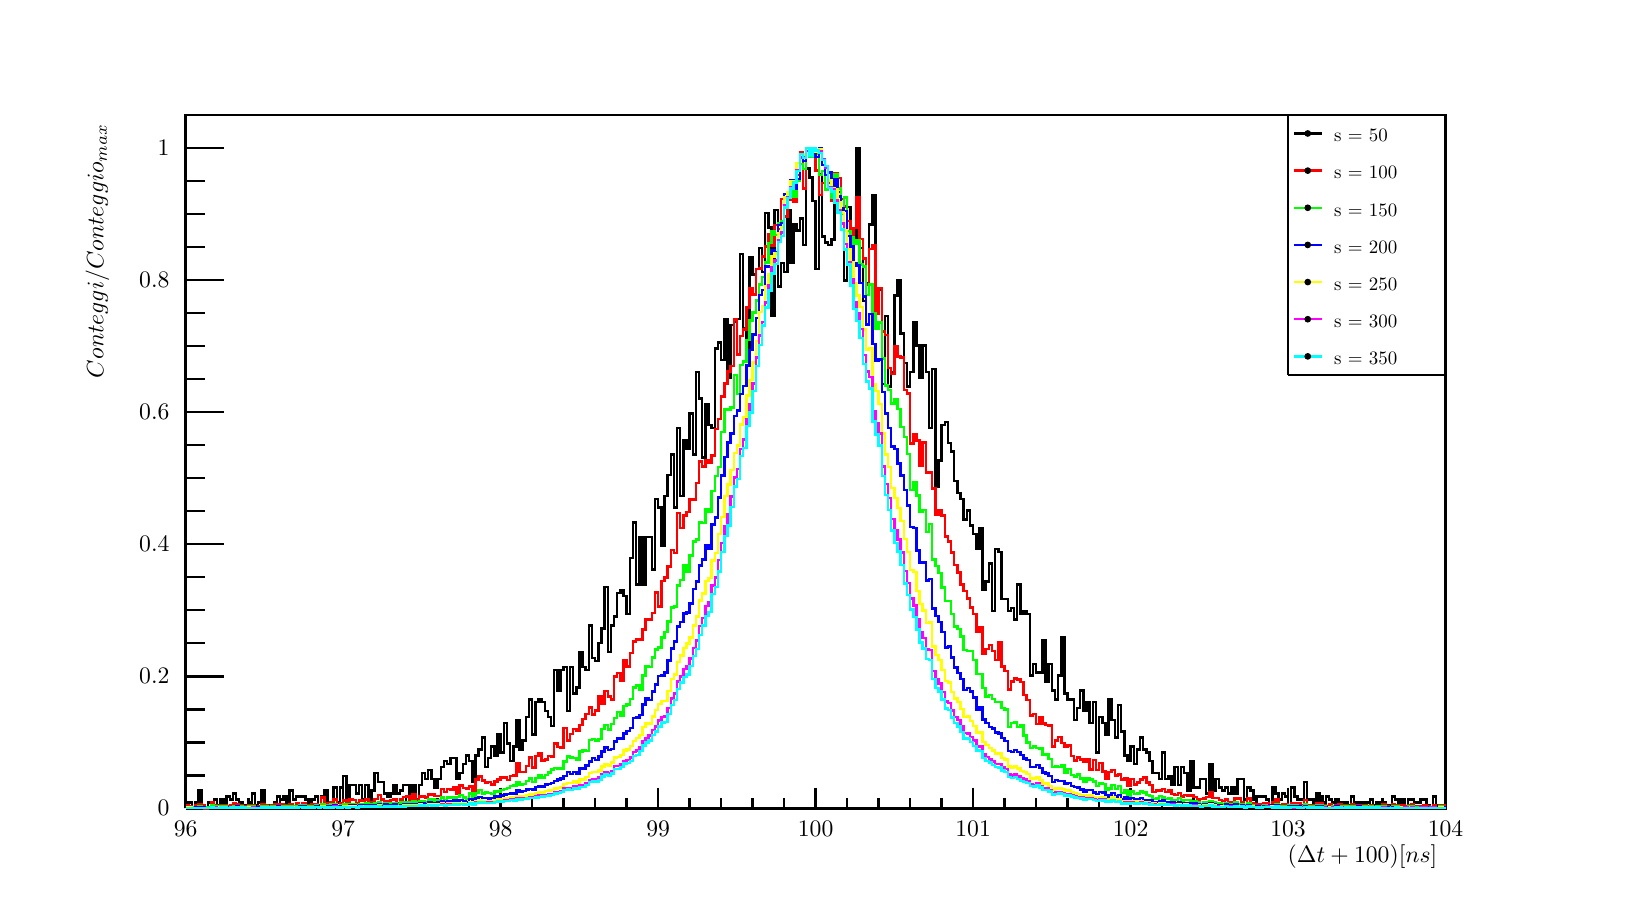
\begin{tikzpicture}
\pgfdeclareplotmark{cross} {
\pgfpathmoveto{\pgfpoint{-0.3\pgfplotmarksize}{\pgfplotmarksize}}
\pgfpathlineto{\pgfpoint{+0.3\pgfplotmarksize}{\pgfplotmarksize}}
\pgfpathlineto{\pgfpoint{+0.3\pgfplotmarksize}{0.3\pgfplotmarksize}}
\pgfpathlineto{\pgfpoint{+1\pgfplotmarksize}{0.3\pgfplotmarksize}}
\pgfpathlineto{\pgfpoint{+1\pgfplotmarksize}{-0.3\pgfplotmarksize}}
\pgfpathlineto{\pgfpoint{+0.3\pgfplotmarksize}{-0.3\pgfplotmarksize}}
\pgfpathlineto{\pgfpoint{+0.3\pgfplotmarksize}{-1.\pgfplotmarksize}}
\pgfpathlineto{\pgfpoint{-0.3\pgfplotmarksize}{-1.\pgfplotmarksize}}
\pgfpathlineto{\pgfpoint{-0.3\pgfplotmarksize}{-0.3\pgfplotmarksize}}
\pgfpathlineto{\pgfpoint{-1.\pgfplotmarksize}{-0.3\pgfplotmarksize}}
\pgfpathlineto{\pgfpoint{-1.\pgfplotmarksize}{0.3\pgfplotmarksize}}
\pgfpathlineto{\pgfpoint{-0.3\pgfplotmarksize}{0.3\pgfplotmarksize}}
\pgfpathclose
\pgfusepathqstroke
}
\pgfdeclareplotmark{cross*} {
\pgfpathmoveto{\pgfpoint{-0.3\pgfplotmarksize}{\pgfplotmarksize}}
\pgfpathlineto{\pgfpoint{+0.3\pgfplotmarksize}{\pgfplotmarksize}}
\pgfpathlineto{\pgfpoint{+0.3\pgfplotmarksize}{0.3\pgfplotmarksize}}
\pgfpathlineto{\pgfpoint{+1\pgfplotmarksize}{0.3\pgfplotmarksize}}
\pgfpathlineto{\pgfpoint{+1\pgfplotmarksize}{-0.3\pgfplotmarksize}}
\pgfpathlineto{\pgfpoint{+0.3\pgfplotmarksize}{-0.3\pgfplotmarksize}}
\pgfpathlineto{\pgfpoint{+0.3\pgfplotmarksize}{-1.\pgfplotmarksize}}
\pgfpathlineto{\pgfpoint{-0.3\pgfplotmarksize}{-1.\pgfplotmarksize}}
\pgfpathlineto{\pgfpoint{-0.3\pgfplotmarksize}{-0.3\pgfplotmarksize}}
\pgfpathlineto{\pgfpoint{-1.\pgfplotmarksize}{-0.3\pgfplotmarksize}}
\pgfpathlineto{\pgfpoint{-1.\pgfplotmarksize}{0.3\pgfplotmarksize}}
\pgfpathlineto{\pgfpoint{-0.3\pgfplotmarksize}{0.3\pgfplotmarksize}}
\pgfpathclose
\pgfusepathqfillstroke
}
\pgfdeclareplotmark{newstar} {
\pgfpathmoveto{\pgfqpoint{0pt}{\pgfplotmarksize}}
\pgfpathlineto{\pgfqpointpolar{44}{0.5\pgfplotmarksize}}
\pgfpathlineto{\pgfqpointpolar{18}{\pgfplotmarksize}}
\pgfpathlineto{\pgfqpointpolar{-20}{0.5\pgfplotmarksize}}
\pgfpathlineto{\pgfqpointpolar{-54}{\pgfplotmarksize}}
\pgfpathlineto{\pgfqpointpolar{-90}{0.5\pgfplotmarksize}}
\pgfpathlineto{\pgfqpointpolar{234}{\pgfplotmarksize}}
\pgfpathlineto{\pgfqpointpolar{198}{0.5\pgfplotmarksize}}
\pgfpathlineto{\pgfqpointpolar{162}{\pgfplotmarksize}}
\pgfpathlineto{\pgfqpointpolar{134}{0.5\pgfplotmarksize}}
\pgfpathclose
\pgfusepathqstroke
}
\pgfdeclareplotmark{newstar*} {
\pgfpathmoveto{\pgfqpoint{0pt}{\pgfplotmarksize}}
\pgfpathlineto{\pgfqpointpolar{44}{0.5\pgfplotmarksize}}
\pgfpathlineto{\pgfqpointpolar{18}{\pgfplotmarksize}}
\pgfpathlineto{\pgfqpointpolar{-20}{0.5\pgfplotmarksize}}
\pgfpathlineto{\pgfqpointpolar{-54}{\pgfplotmarksize}}
\pgfpathlineto{\pgfqpointpolar{-90}{0.5\pgfplotmarksize}}
\pgfpathlineto{\pgfqpointpolar{234}{\pgfplotmarksize}}
\pgfpathlineto{\pgfqpointpolar{198}{0.5\pgfplotmarksize}}
\pgfpathlineto{\pgfqpointpolar{162}{\pgfplotmarksize}}
\pgfpathlineto{\pgfqpointpolar{134}{0.5\pgfplotmarksize}}
\pgfpathclose
\pgfusepathqfillstroke
}
\definecolor{c}{rgb}{1,1,1};
\draw [color=c, fill=c] (0,0) rectangle (20,11.0085);
\draw [color=c, fill=c] (2,1.10085) rectangle (18,9.90762);
\definecolor{c}{rgb}{0,0,0};
\draw [c,line width=0.9] (2,1.10085) -- (2,9.90762) -- (18,9.90762) -- (18,1.10085) -- (2,1.10085);
\definecolor{c}{rgb}{1,1,1};
\draw [color=c, fill=c] (2,1.10085) rectangle (18,9.90762);
\definecolor{c}{rgb}{0,0,0};
\draw [c,line width=0.9] (2,1.10085) -- (2,9.90762) -- (18,9.90762) -- (18,1.10085) -- (2,1.10085);
\draw [c,line width=0.9] (2,1.17573) -- (2.04,1.17573) -- (2.04,1.17573) -- (2.08,1.17573) -- (2.08,1.10085) -- (2.12,1.10085) -- (2.12,1.17573) -- (2.16,1.17573) -- (2.16,1.32551) -- (2.2,1.32551) -- (2.2,1.13829) -- (2.24,1.13829) -- (2.24,1.10085)
 -- (2.28,1.10085) -- (2.28,1.17573) -- (2.32,1.17573) -- (2.32,1.17573) -- (2.36,1.17573) -- (2.36,1.21318) -- (2.4,1.21318) -- (2.4,1.13829) -- (2.44,1.13829) -- (2.44,1.21318) -- (2.48,1.21318) -- (2.48,1.17573) -- (2.52,1.17573) -- (2.52,1.25062)
 -- (2.56,1.25062) -- (2.56,1.21318) -- (2.6,1.21318) -- (2.6,1.28807) -- (2.64,1.28807) -- (2.64,1.21318) -- (2.68,1.21318) -- (2.68,1.17573) -- (2.72,1.17573) -- (2.72,1.13829) -- (2.76,1.13829) -- (2.76,1.13829) -- (2.8,1.13829) -- (2.8,1.17573)
 -- (2.84,1.17573) -- (2.84,1.28807) -- (2.88,1.28807) -- (2.88,1.13829) -- (2.92,1.13829) -- (2.92,1.17573) -- (2.96,1.17573) -- (2.96,1.32551) -- (3,1.32551) -- (3,1.13829) -- (3.04,1.13829) -- (3.04,1.13829) -- (3.08,1.13829) -- (3.08,1.13829) --
 (3.12,1.13829) -- (3.12,1.17573) -- (3.16,1.17573) -- (3.16,1.25062) -- (3.2,1.25062) -- (3.2,1.21318) -- (3.24,1.21318) -- (3.24,1.25062) -- (3.28,1.25062) -- (3.28,1.13829) -- (3.32,1.13829) -- (3.32,1.32551) -- (3.36,1.32551) -- (3.36,1.21318) --
 (3.4,1.21318) -- (3.4,1.25062) -- (3.44,1.25062) -- (3.44,1.25062) -- (3.48,1.25062) -- (3.48,1.25062) -- (3.52,1.25062) -- (3.52,1.21318) -- (3.56,1.21318) -- (3.56,1.17573) -- (3.6,1.17573) -- (3.6,1.21318) -- (3.64,1.21318) -- (3.64,1.25062) --
 (3.68,1.25062) -- (3.68,1.13829) -- (3.72,1.13829) -- (3.72,1.25062) -- (3.76,1.25062) -- (3.76,1.32551) -- (3.8,1.32551) -- (3.8,1.17573) -- (3.84,1.17573) -- (3.84,1.17573) -- (3.88,1.17573) -- (3.88,1.36295) -- (3.92,1.36295) -- (3.92,1.17573) --
 (3.96,1.17573) -- (3.96,1.36295) -- (4,1.36295) -- (4,1.51273) -- (4.04,1.51273) -- (4.04,1.13829) -- (4.08,1.13829) -- (4.08,1.4004) -- (4.12,1.4004) -- (4.12,1.4004) -- (4.16,1.4004) -- (4.16,1.28807) -- (4.2,1.28807) -- (4.2,1.4004) --
 (4.24,1.4004) -- (4.24,1.21318) -- (4.28,1.21318) -- (4.28,1.4004) -- (4.32,1.4004) -- (4.32,1.21318) -- (4.36,1.21318) -- (4.36,1.32551) -- (4.4,1.32551) -- (4.4,1.55017) -- (4.44,1.55017) -- (4.44,1.43784) -- (4.48,1.43784) -- (4.48,1.43784) --
 (4.52,1.43784) -- (4.52,1.28807) -- (4.56,1.28807) -- (4.56,1.25062) -- (4.6,1.25062) -- (4.6,1.28807) -- (4.64,1.28807) -- (4.64,1.4004) -- (4.68,1.4004) -- (4.68,1.28807) -- (4.72,1.28807) -- (4.72,1.32551) -- (4.76,1.32551) -- (4.76,1.4004) --
 (4.8,1.4004) -- (4.8,1.4004) -- (4.84,1.4004) -- (4.84,1.25062) -- (4.88,1.25062) -- (4.88,1.4004) -- (4.92,1.4004) -- (4.92,1.21318) -- (4.96,1.21318) -- (4.96,1.4004) -- (5,1.4004) -- (5,1.55017) -- (5.04,1.55017) -- (5.04,1.47528) --
 (5.08,1.47528) -- (5.08,1.58762) -- (5.12,1.58762) -- (5.12,1.47528) -- (5.16,1.47528) -- (5.16,1.36295) -- (5.2,1.36295) -- (5.2,1.47528) -- (5.24,1.47528) -- (5.24,1.62506) -- (5.28,1.62506) -- (5.28,1.69995) -- (5.32,1.69995) -- (5.32,1.6625) --
 (5.36,1.6625) -- (5.36,1.73739) -- (5.4,1.73739) -- (5.4,1.73739) -- (5.44,1.73739) -- (5.44,1.47528) -- (5.48,1.47528) -- (5.48,1.55017) -- (5.52,1.55017) -- (5.52,1.6625) -- (5.56,1.6625) -- (5.56,1.77483) -- (5.6,1.77483) -- (5.6,1.69995) --
 (5.64,1.69995) -- (5.64,1.43784) -- (5.68,1.43784) -- (5.68,1.77483) -- (5.72,1.77483) -- (5.72,1.84972) -- (5.76,1.84972) -- (5.76,1.9995) -- (5.8,1.9995) -- (5.8,1.62506) -- (5.84,1.62506) -- (5.84,1.73739) -- (5.88,1.73739) -- (5.88,1.88717) --
 (5.92,1.88717) -- (5.92,1.77483) -- (5.96,1.77483) -- (5.96,2.03694) -- (6,2.03694) -- (6,1.81228) -- (6.04,1.81228) -- (6.04,2.18672) -- (6.08,2.18672) -- (6.08,1.92461) -- (6.12,1.92461) -- (6.12,1.69995) -- (6.16,1.69995) -- (6.16,1.88717) --
 (6.2,1.88717) -- (6.2,2.22416) -- (6.24,2.22416) -- (6.24,1.84972) -- (6.28,1.84972) -- (6.28,1.96205) -- (6.32,1.96205) -- (6.32,2.2616) -- (6.36,2.2616) -- (6.36,2.48627) -- (6.4,2.48627) -- (6.4,2.03694) -- (6.44,2.03694) -- (6.44,2.44882) --
 (6.48,2.44882) -- (6.48,2.48627) -- (6.52,2.48627) -- (6.52,2.44882) -- (6.56,2.44882) -- (6.56,2.33649) -- (6.6,2.33649) -- (6.6,2.2616) -- (6.64,2.2616) -- (6.64,2.14927) -- (6.68,2.14927) -- (6.68,2.8607) -- (6.72,2.8607) -- (6.72,2.5986) --
 (6.76,2.5986) -- (6.76,2.8607) -- (6.8,2.8607) -- (6.8,2.89815) -- (6.84,2.89815) -- (6.84,2.33649) -- (6.88,2.33649) -- (6.88,2.89815) -- (6.92,2.89815) -- (6.92,2.56115) -- (6.96,2.56115) -- (6.96,2.63604) -- (7,2.63604) -- (7,3.08537) --
 (7.04,3.08537) -- (7.04,2.89815) -- (7.08,2.89815) -- (7.08,2.8607) -- (7.12,2.8607) -- (7.12,3.42236) -- (7.16,3.42236) -- (7.16,3.01048) -- (7.2,3.01048) -- (7.2,2.97304) -- (7.24,2.97304) -- (7.24,3.1977) -- (7.28,3.1977) -- (7.28,3.38492) --
 (7.32,3.38492) -- (7.32,3.90913) -- (7.36,3.90913) -- (7.36,3.08537) -- (7.4,3.08537) -- (7.4,3.42236) -- (7.44,3.42236) -- (7.44,3.53469) -- (7.48,3.53469) -- (7.48,3.83424) -- (7.52,3.83424) -- (7.52,3.87169) -- (7.56,3.87169) -- (7.56,3.7968) --
 (7.6,3.7968) -- (7.6,3.57214) -- (7.64,3.57214) -- (7.64,4.28357) -- (7.68,4.28357) -- (7.68,4.73289) -- (7.72,4.73289) -- (7.72,3.94657) -- (7.76,3.94657) -- (7.76,4.54567) -- (7.8,4.54567) -- (7.8,3.94657) -- (7.84,3.94657) -- (7.84,4.54567) --
 (7.88,4.54567) -- (7.88,4.54567) -- (7.92,4.54567) -- (7.92,4.13379) -- (7.96,4.13379) -- (7.96,5.03244) -- (8,5.03244) -- (8,4.92011) -- (8.04,4.92011) -- (8.04,4.43334) -- (8.08,4.43334) -- (8.08,5.06989) -- (8.12,5.06989) -- (8.12,5.33199) --
 (8.16,5.33199) -- (8.16,5.5941) -- (8.2,5.5941) -- (8.2,4.92011) -- (8.24,4.92011) -- (8.24,5.93109) -- (8.28,5.93109) -- (8.28,5.06989) -- (8.32,5.06989) -- (8.32,5.78132) -- (8.36,5.78132) -- (8.36,5.66899) -- (8.4,5.66899) -- (8.4,6.11831) --
 (8.44,6.11831) -- (8.44,5.5941) -- (8.48,5.5941) -- (8.48,6.64252) -- (8.52,6.64252) -- (8.52,6.30553) -- (8.56,6.30553) -- (8.56,5.55665) -- (8.6,5.55665) -- (8.6,6.23064) -- (8.64,6.23064) -- (8.64,5.96854) -- (8.68,5.96854) -- (8.68,5.93109) --
 (8.72,5.93109) -- (8.72,6.94207) -- (8.76,6.94207) -- (8.76,7.01696) -- (8.8,7.01696) -- (8.8,6.7923) -- (8.84,6.7923) -- (8.84,7.31651) -- (8.88,7.31651) -- (8.88,6.56764) -- (8.92,6.56764) -- (8.92,7.24162) -- (8.96,7.24162) -- (8.96,7.27907) --
 (9,7.27907) -- (9,7.31651) -- (9.04,7.31651) -- (9.04,8.14028) -- (9.08,8.14028) -- (9.08,7.20418) -- (9.12,7.20418) -- (9.12,6.86719) -- (9.16,6.86719) -- (9.16,8.10283) -- (9.2,8.10283) -- (9.2,7.87817) -- (9.24,7.87817) -- (9.24,7.95306) --
 (9.28,7.95306) -- (9.28,8.21516) -- (9.32,8.21516) -- (9.32,7.91561) -- (9.36,7.91561) -- (9.36,8.66449) -- (9.4,8.66449) -- (9.4,8.47727) -- (9.44,8.47727) -- (9.44,7.35396) -- (9.48,7.35396) -- (9.48,8.70193) -- (9.52,8.70193) -- (9.52,7.72839) --
 (9.56,7.72839) -- (9.56,8.02794) -- (9.6,8.02794) -- (9.6,7.91561) -- (9.64,7.91561) -- (9.64,8.70193) -- (9.68,8.70193) -- (9.68,8.02794) -- (9.72,8.02794) -- (9.72,8.51471) -- (9.76,8.51471) -- (9.76,8.43983) -- (9.8,8.43983) -- (9.8,8.5896) --
 (9.84,8.5896) -- (9.84,8.25261) -- (9.88,8.25261) -- (9.88,9.22614) -- (9.92,9.22614) -- (9.92,9.11381) -- (9.96,9.11381) -- (9.96,8.81426) -- (10,8.81426) -- (10,7.95306) -- (10.04,7.95306) -- (10.04,9.15126) -- (10.08,9.15126) -- (10.08,8.36494)
 -- (10.12,8.36494) -- (10.12,8.29005) -- (10.16,8.29005) -- (10.16,8.25261) -- (10.2,8.25261) -- (10.2,8.32749) -- (10.24,8.32749) -- (10.24,8.88915) -- (10.28,8.88915) -- (10.28,8.92659) -- (10.32,8.92659) -- (10.32,8.70193) -- (10.36,8.70193) --
 (10.36,7.80328) -- (10.4,7.80328) -- (10.4,8.73938) -- (10.44,8.73938) -- (10.44,8.06539) -- (10.48,8.06539) -- (10.48,8.29005) -- (10.52,8.29005) -- (10.52,9.48825) -- (10.56,9.48825) -- (10.56,8.21516) -- (10.6,8.21516) -- (10.6,7.54117) --
 (10.64,7.54117) -- (10.64,7.76584) -- (10.68,7.76584) -- (10.68,8.51471) -- (10.72,8.51471) -- (10.72,8.88915) -- (10.76,8.88915) -- (10.76,7.46629) -- (10.8,7.46629) -- (10.8,7.69095) -- (10.84,7.69095) -- (10.84,6.49275) -- (10.88,6.49275) --
 (10.88,7.35396) -- (10.92,7.35396) -- (10.92,6.45531) -- (10.96,6.45531) -- (10.96,6.64252) -- (11,6.64252) -- (11,7.61606) -- (11.04,7.61606) -- (11.04,7.80328) -- (11.08,7.80328) -- (11.08,7.12929) -- (11.12,7.12929) -- (11.12,6.75486) --
 (11.16,6.75486) -- (11.16,6.45531) -- (11.2,6.45531) -- (11.2,6.64252) -- (11.24,6.64252) -- (11.24,7.27907) -- (11.28,7.27907) -- (11.28,6.97952) -- (11.32,6.97952) -- (11.32,6.56764) -- (11.36,6.56764) -- (11.36,6.97952) -- (11.4,6.97952) --
 (11.4,6.64252) -- (11.44,6.64252) -- (11.44,5.93109) -- (11.48,5.93109) -- (11.48,6.67997) -- (11.52,6.67997) -- (11.52,5.18222) -- (11.56,5.18222) -- (11.56,5.51921) -- (11.6,5.51921) -- (11.6,5.96854) -- (11.64,5.96854) -- (11.64,6.00598) --
 (11.68,6.00598) -- (11.68,5.74387) -- (11.72,5.74387) -- (11.72,5.63154) -- (11.76,5.63154) -- (11.76,5.2571) -- (11.8,5.2571) -- (11.8,5.10733) -- (11.84,5.10733) -- (11.84,5.03244) -- (11.88,5.03244) -- (11.88,4.77034) -- (11.92,4.77034) --
 (11.92,4.88267) -- (11.96,4.88267) -- (11.96,4.69545) -- (12,4.69545) -- (12,4.58312) -- (12.04,4.58312) -- (12.04,4.3959) -- (12.08,4.3959) -- (12.08,4.658) -- (12.12,4.658) -- (12.12,3.87169) -- (12.16,3.87169) -- (12.16,3.98402) -- (12.2,3.98402)
 -- (12.2,4.20868) -- (12.24,4.20868) -- (12.24,3.60958) -- (12.28,3.60958) -- (12.28,4.3959) -- (12.32,4.3959) -- (12.32,4.35845) -- (12.36,4.35845) -- (12.36,3.75935) -- (12.4,3.75935) -- (12.4,3.75935) -- (12.44,3.75935) -- (12.44,3.60958) --
 (12.48,3.60958) -- (12.48,3.64702) -- (12.52,3.64702) -- (12.52,3.49725) -- (12.56,3.49725) -- (12.56,3.94657) -- (12.6,3.94657) -- (12.6,3.57214) -- (12.64,3.57214) -- (12.64,3.60958) -- (12.68,3.60958) -- (12.68,3.57214) -- (12.72,3.57214) --
 (12.72,2.78582) -- (12.76,2.78582) -- (12.76,2.93559) -- (12.8,2.93559) -- (12.8,2.82326) -- (12.84,2.82326) -- (12.84,2.82326) -- (12.88,2.82326) -- (12.88,3.23514) -- (12.92,3.23514) -- (12.92,2.71093) -- (12.96,2.71093) -- (12.96,2.93559) --
 (13,2.93559) -- (13,2.5986) -- (13.04,2.5986) -- (13.04,2.48627) -- (13.08,2.48627) -- (13.08,2.78582) -- (13.12,2.78582) -- (13.12,3.27259) -- (13.16,3.27259) -- (13.16,2.56115) -- (13.2,2.56115) -- (13.2,2.48627) -- (13.24,2.48627) --
 (13.24,2.48627) -- (13.28,2.48627) -- (13.28,2.22416) -- (13.32,2.22416) -- (13.32,2.37393) -- (13.36,2.37393) -- (13.36,2.5986) -- (13.4,2.5986) -- (13.4,2.33649) -- (13.44,2.33649) -- (13.44,2.44882) -- (13.48,2.44882) -- (13.48,2.18672) --
 (13.52,2.18672) -- (13.52,2.44882) -- (13.56,2.44882) -- (13.56,1.81228) -- (13.6,1.81228) -- (13.6,2.2616) -- (13.64,2.2616) -- (13.64,2.18672) -- (13.68,2.18672) -- (13.68,2.03694) -- (13.72,2.03694) -- (13.72,2.48627) -- (13.76,2.48627) --
 (13.76,2.22416) -- (13.8,2.22416) -- (13.8,1.9995) -- (13.84,1.9995) -- (13.84,2.41138) -- (13.88,2.41138) -- (13.88,2.07438) -- (13.92,2.07438) -- (13.92,1.77483) -- (13.96,1.77483) -- (13.96,1.69995) -- (14,1.69995) -- (14,1.88717) --
 (14.04,1.88717) -- (14.04,1.6625) -- (14.08,1.6625) -- (14.08,1.84972) -- (14.12,1.84972) -- (14.12,1.9995) -- (14.16,1.9995) -- (14.16,1.84972) -- (14.2,1.84972) -- (14.2,1.81228) -- (14.24,1.81228) -- (14.24,1.69995) -- (14.28,1.69995) --
 (14.28,1.55017) -- (14.32,1.55017) -- (14.32,1.55017) -- (14.36,1.55017) -- (14.36,1.47528) -- (14.4,1.47528) -- (14.4,1.81228) -- (14.44,1.81228) -- (14.44,1.47528) -- (14.48,1.47528) -- (14.48,1.51273) -- (14.52,1.51273) -- (14.52,1.4004) --
 (14.56,1.4004) -- (14.56,1.62506) -- (14.6,1.62506) -- (14.6,1.4004) -- (14.64,1.4004) -- (14.64,1.62506) -- (14.68,1.62506) -- (14.68,1.55017) -- (14.72,1.55017) -- (14.72,1.32551) -- (14.76,1.32551) -- (14.76,1.69995) -- (14.8,1.69995) --
 (14.8,1.36295) -- (14.84,1.36295) -- (14.84,1.36295) -- (14.88,1.36295) -- (14.88,1.47528) -- (14.92,1.47528) -- (14.92,1.47528) -- (14.96,1.47528) -- (14.96,1.28807) -- (15,1.28807) -- (15,1.6625) -- (15.04,1.6625) -- (15.04,1.32551) --
 (15.08,1.32551) -- (15.08,1.47528) -- (15.12,1.47528) -- (15.12,1.36295) -- (15.16,1.36295) -- (15.16,1.32551) -- (15.2,1.32551) -- (15.2,1.36295) -- (15.24,1.36295) -- (15.24,1.28807) -- (15.28,1.28807) -- (15.28,1.36295) -- (15.32,1.36295) --
 (15.32,1.28807) -- (15.36,1.28807) -- (15.36,1.47528) -- (15.4,1.47528) -- (15.4,1.47528) -- (15.44,1.47528) -- (15.44,1.21318) -- (15.48,1.21318) -- (15.48,1.36295) -- (15.52,1.36295) -- (15.52,1.32551) -- (15.56,1.32551) -- (15.56,1.21318) --
 (15.6,1.21318) -- (15.6,1.25062) -- (15.64,1.25062) -- (15.64,1.25062) -- (15.68,1.25062) -- (15.68,1.25062) -- (15.72,1.25062) -- (15.72,1.21318) -- (15.76,1.21318) -- (15.76,1.13829) -- (15.8,1.13829) -- (15.8,1.36295) -- (15.84,1.36295) --
 (15.84,1.28807) -- (15.88,1.28807) -- (15.88,1.21318) -- (15.92,1.21318) -- (15.92,1.28807) -- (15.96,1.28807) -- (15.96,1.25062) -- (16,1.25062) -- (16,1.13829) -- (16.04,1.13829) -- (16.04,1.36295) -- (16.08,1.36295) -- (16.08,1.25062) --
 (16.12,1.25062) -- (16.12,1.21318) -- (16.16,1.21318) -- (16.16,1.21318) -- (16.2,1.21318) -- (16.2,1.43784) -- (16.24,1.43784) -- (16.24,1.21318) -- (16.28,1.21318) -- (16.28,1.21318) -- (16.32,1.21318) -- (16.32,1.13829) -- (16.36,1.13829) --
 (16.36,1.28807) -- (16.4,1.28807) -- (16.4,1.25062) -- (16.44,1.25062) -- (16.44,1.17573) -- (16.48,1.17573) -- (16.48,1.25062) -- (16.52,1.25062) -- (16.52,1.21318) -- (16.56,1.21318) -- (16.56,1.17573) -- (16.6,1.17573) -- (16.6,1.21318) --
 (16.64,1.21318) -- (16.64,1.13829) -- (16.68,1.13829) -- (16.68,1.17573) -- (16.72,1.17573) -- (16.72,1.17573) -- (16.76,1.17573) -- (16.76,1.13829) -- (16.8,1.13829) -- (16.8,1.25062) -- (16.84,1.25062) -- (16.84,1.17573) -- (16.88,1.17573) --
 (16.88,1.17573) -- (16.92,1.17573) -- (16.92,1.17573) -- (16.96,1.17573) -- (16.96,1.17573) -- (17,1.17573) -- (17,1.17573) -- (17.04,1.17573) -- (17.04,1.21318) -- (17.08,1.21318) -- (17.08,1.13829) -- (17.12,1.13829) -- (17.12,1.17573) --
 (17.16,1.17573) -- (17.16,1.13829) -- (17.2,1.13829) -- (17.2,1.17573) -- (17.24,1.17573) -- (17.24,1.13829) -- (17.28,1.13829) -- (17.28,1.13829) -- (17.32,1.13829) -- (17.32,1.25062) -- (17.36,1.25062) -- (17.36,1.21318) -- (17.4,1.21318) --
 (17.4,1.13829) -- (17.44,1.13829) -- (17.44,1.21318) -- (17.48,1.21318) -- (17.48,1.10085) -- (17.52,1.10085) -- (17.52,1.21318) -- (17.56,1.21318) -- (17.56,1.21318) -- (17.6,1.21318) -- (17.6,1.17573) -- (17.64,1.17573) -- (17.64,1.17573) --
 (17.68,1.17573) -- (17.68,1.21318) -- (17.72,1.21318) -- (17.72,1.21318) -- (17.76,1.21318) -- (17.76,1.13829) -- (17.8,1.13829) -- (17.8,1.10085) -- (17.84,1.10085) -- (17.84,1.25062) -- (17.88,1.25062) -- (17.88,1.13829) -- (17.92,1.13829) --
 (17.92,1.10085) -- (17.96,1.10085) -- (17.96,1.10085) -- (18,1.10085);
\draw [c,line width=0.9] (2,1.10085) -- (18,1.10085);
\draw [anchor= east] (18,0.484373) node[scale=0.854877, color=c, rotate=0]{$(\Delta t + 100) [ns]$};
\draw [c,line width=0.9] (2,1.36505) -- (2,1.10085);
\draw [c,line width=0.9] (2.4,1.23295) -- (2.4,1.10085);
\draw [c,line width=0.9] (2.8,1.23295) -- (2.8,1.10085);
\draw [c,line width=0.9] (3.2,1.23295) -- (3.2,1.10085);
\draw [c,line width=0.9] (3.6,1.23295) -- (3.6,1.10085);
\draw [c,line width=0.9] (4,1.36505) -- (4,1.10085);
\draw [c,line width=0.9] (4.4,1.23295) -- (4.4,1.10085);
\draw [c,line width=0.9] (4.8,1.23295) -- (4.8,1.10085);
\draw [c,line width=0.9] (5.2,1.23295) -- (5.2,1.10085);
\draw [c,line width=0.9] (5.6,1.23295) -- (5.6,1.10085);
\draw [c,line width=0.9] (6,1.36505) -- (6,1.10085);
\draw [c,line width=0.9] (6.4,1.23295) -- (6.4,1.10085);
\draw [c,line width=0.9] (6.8,1.23295) -- (6.8,1.10085);
\draw [c,line width=0.9] (7.2,1.23295) -- (7.2,1.10085);
\draw [c,line width=0.9] (7.6,1.23295) -- (7.6,1.10085);
\draw [c,line width=0.9] (8,1.36505) -- (8,1.10085);
\draw [c,line width=0.9] (8.4,1.23295) -- (8.4,1.10085);
\draw [c,line width=0.9] (8.8,1.23295) -- (8.8,1.10085);
\draw [c,line width=0.9] (9.2,1.23295) -- (9.2,1.10085);
\draw [c,line width=0.9] (9.6,1.23295) -- (9.6,1.10085);
\draw [c,line width=0.9] (10,1.36505) -- (10,1.10085);
\draw [c,line width=0.9] (10.4,1.23295) -- (10.4,1.10085);
\draw [c,line width=0.9] (10.8,1.23295) -- (10.8,1.10085);
\draw [c,line width=0.9] (11.2,1.23295) -- (11.2,1.10085);
\draw [c,line width=0.9] (11.6,1.23295) -- (11.6,1.10085);
\draw [c,line width=0.9] (12,1.36505) -- (12,1.10085);
\draw [c,line width=0.9] (12.4,1.23295) -- (12.4,1.10085);
\draw [c,line width=0.9] (12.8,1.23295) -- (12.8,1.10085);
\draw [c,line width=0.9] (13.2,1.23295) -- (13.2,1.10085);
\draw [c,line width=0.9] (13.6,1.23295) -- (13.6,1.10085);
\draw [c,line width=0.9] (14,1.36505) -- (14,1.10085);
\draw [c,line width=0.9] (14.4,1.23295) -- (14.4,1.10085);
\draw [c,line width=0.9] (14.8,1.23295) -- (14.8,1.10085);
\draw [c,line width=0.9] (15.2,1.23295) -- (15.2,1.10085);
\draw [c,line width=0.9] (15.6,1.23295) -- (15.6,1.10085);
\draw [c,line width=0.9] (16,1.36505) -- (16,1.10085);
\draw [c,line width=0.9] (16.4,1.23295) -- (16.4,1.10085);
\draw [c,line width=0.9] (16.8,1.23295) -- (16.8,1.10085);
\draw [c,line width=0.9] (17.2,1.23295) -- (17.2,1.10085);
\draw [c,line width=0.9] (17.6,1.23295) -- (17.6,1.10085);
\draw [c,line width=0.9] (18,1.36505) -- (18,1.10085);
\draw [anchor=base] (2,0.737567) node[scale=0.854877, color=c, rotate=0]{96};
\draw [anchor=base] (4,0.737567) node[scale=0.854877, color=c, rotate=0]{97};
\draw [anchor=base] (6,0.737567) node[scale=0.854877, color=c, rotate=0]{98};
\draw [anchor=base] (8,0.737567) node[scale=0.854877, color=c, rotate=0]{99};
\draw [anchor=base] (10,0.737567) node[scale=0.854877, color=c, rotate=0]{100};
\draw [anchor=base] (12,0.737567) node[scale=0.854877, color=c, rotate=0]{101};
\draw [anchor=base] (14,0.737567) node[scale=0.854877, color=c, rotate=0]{102};
\draw [anchor=base] (16,0.737567) node[scale=0.854877, color=c, rotate=0]{103};
\draw [anchor=base] (18,0.737567) node[scale=0.854877, color=c, rotate=0]{104};
\draw [c,line width=0.9] (2,1.10085) -- (2,9.90762);
\draw [anchor= east] (0.88,9.90762) node[scale=0.854877, color=c, rotate=90]{$Conteggi/Conteggio_{max}$};
\draw [c,line width=0.9] (2.48,1.10085) -- (2,1.10085);
\draw [c,line width=0.9] (2.24,1.52022) -- (2,1.52022);
\draw [c,line width=0.9] (2.24,1.93959) -- (2,1.93959);
\draw [c,line width=0.9] (2.24,2.35896) -- (2,2.35896);
\draw [c,line width=0.9] (2.48,2.77833) -- (2,2.77833);
\draw [c,line width=0.9] (2.24,3.1977) -- (2,3.1977);
\draw [c,line width=0.9] (2.24,3.61707) -- (2,3.61707);
\draw [c,line width=0.9] (2.24,4.03644) -- (2,4.03644);
\draw [c,line width=0.9] (2.48,4.45581) -- (2,4.45581);
\draw [c,line width=0.9] (2.24,4.87518) -- (2,4.87518);
\draw [c,line width=0.9] (2.24,5.29455) -- (2,5.29455);
\draw [c,line width=0.9] (2.24,5.71392) -- (2,5.71392);
\draw [c,line width=0.9] (2.48,6.13329) -- (2,6.13329);
\draw [c,line width=0.9] (2.24,6.55266) -- (2,6.55266);
\draw [c,line width=0.9] (2.24,6.97203) -- (2,6.97203);
\draw [c,line width=0.9] (2.24,7.3914) -- (2,7.3914);
\draw [c,line width=0.9] (2.48,7.81077) -- (2,7.81077);
\draw [c,line width=0.9] (2.24,8.23014) -- (2,8.23014);
\draw [c,line width=0.9] (2.24,8.64951) -- (2,8.64951);
\draw [c,line width=0.9] (2.24,9.06888) -- (2,9.06888);
\draw [c,line width=0.9] (2.48,9.48825) -- (2,9.48825);
\draw [c,line width=0.9] (2.48,9.48825) -- (2,9.48825);
\draw [anchor= east] (1.9,1.10085) node[scale=0.854877, color=c, rotate=0]{0};
\draw [anchor= east] (1.9,2.77833) node[scale=0.854877, color=c, rotate=0]{0.2};
\draw [anchor= east] (1.9,4.45581) node[scale=0.854877, color=c, rotate=0]{0.4};
\draw [anchor= east] (1.9,6.13329) node[scale=0.854877, color=c, rotate=0]{0.6};
\draw [anchor= east] (1.9,7.81077) node[scale=0.854877, color=c, rotate=0]{0.8};
\draw [anchor= east] (1.9,9.48825) node[scale=0.854877, color=c, rotate=0]{1};
\definecolor{c}{rgb}{1,0,0};
\draw [c,line width=0.9] (2,1.13562) -- (2.04,1.13562) -- (2.04,1.12171) -- (2.08,1.12171) -- (2.08,1.1078) -- (2.12,1.1078) -- (2.12,1.13562) -- (2.16,1.13562) -- (2.16,1.14953) -- (2.2,1.14953) -- (2.2,1.13562) -- (2.24,1.13562) -- (2.24,1.10085)
 -- (2.28,1.10085) -- (2.28,1.11476) -- (2.32,1.11476) -- (2.32,1.17735) -- (2.36,1.17735) -- (2.36,1.14258) -- (2.4,1.14258) -- (2.4,1.12867) -- (2.44,1.12867) -- (2.44,1.14258) -- (2.48,1.14258) -- (2.48,1.13562) -- (2.52,1.13562) -- (2.52,1.12867)
 -- (2.56,1.12867) -- (2.56,1.14258) -- (2.6,1.14258) -- (2.6,1.16344) -- (2.64,1.16344) -- (2.64,1.14953) -- (2.68,1.14953) -- (2.68,1.14258) -- (2.72,1.14258) -- (2.72,1.11476) -- (2.76,1.11476) -- (2.76,1.12171) -- (2.8,1.12171) -- (2.8,1.14258)
 -- (2.84,1.14258) -- (2.84,1.14258) -- (2.88,1.14258) -- (2.88,1.11476) -- (2.92,1.11476) -- (2.92,1.12171) -- (2.96,1.12171) -- (2.96,1.14953) -- (3,1.14953) -- (3,1.14258) -- (3.04,1.14258) -- (3.04,1.12867) -- (3.08,1.12867) -- (3.08,1.13562) --
 (3.12,1.13562) -- (3.12,1.14953) -- (3.16,1.14953) -- (3.16,1.14953) -- (3.2,1.14953) -- (3.2,1.14953) -- (3.24,1.14953) -- (3.24,1.13562) -- (3.28,1.13562) -- (3.28,1.12171) -- (3.32,1.12171) -- (3.32,1.14953) -- (3.36,1.14953) -- (3.36,1.12171) --
 (3.4,1.12171) -- (3.4,1.16344) -- (3.44,1.16344) -- (3.44,1.13562) -- (3.48,1.13562) -- (3.48,1.17039) -- (3.52,1.17039) -- (3.52,1.12867) -- (3.56,1.12867) -- (3.56,1.13562) -- (3.6,1.13562) -- (3.6,1.14953) -- (3.64,1.14953) -- (3.64,1.14953) --
 (3.68,1.14953) -- (3.68,1.11476) -- (3.72,1.11476) -- (3.72,1.23994) -- (3.76,1.23994) -- (3.76,1.16344) -- (3.8,1.16344) -- (3.8,1.14953) -- (3.84,1.14953) -- (3.84,1.1843) -- (3.88,1.1843) -- (3.88,1.21212) -- (3.92,1.21212) -- (3.92,1.12171) --
 (3.96,1.12171) -- (3.96,1.16344) -- (4,1.16344) -- (4,1.19821) -- (4.04,1.19821) -- (4.04,1.14258) -- (4.08,1.14258) -- (4.08,1.21212) -- (4.12,1.21212) -- (4.12,1.20517) -- (4.16,1.20517) -- (4.16,1.16344) -- (4.2,1.16344) -- (4.2,1.19821) --
 (4.24,1.19821) -- (4.24,1.19126) -- (4.28,1.19126) -- (4.28,1.21212) -- (4.32,1.21212) -- (4.32,1.17039) -- (4.36,1.17039) -- (4.36,1.1843) -- (4.4,1.1843) -- (4.4,1.21908) -- (4.44,1.21908) -- (4.44,1.26776) -- (4.48,1.26776) -- (4.48,1.21212) --
 (4.52,1.21212) -- (4.52,1.19126) -- (4.56,1.19126) -- (4.56,1.16344) -- (4.6,1.16344) -- (4.6,1.20517) -- (4.64,1.20517) -- (4.64,1.21212) -- (4.68,1.21212) -- (4.68,1.17039) -- (4.72,1.17039) -- (4.72,1.21212) -- (4.76,1.21212) -- (4.76,1.2469) --
 (4.8,1.2469) -- (4.8,1.25385) -- (4.84,1.25385) -- (4.84,1.21212) -- (4.88,1.21212) -- (4.88,1.27472) -- (4.92,1.27472) -- (4.92,1.19821) -- (4.96,1.19821) -- (4.96,1.25385) -- (5,1.25385) -- (5,1.25385) -- (5.04,1.25385) -- (5.04,1.23994) --
 (5.08,1.23994) -- (5.08,1.27472) -- (5.12,1.27472) -- (5.12,1.28167) -- (5.16,1.28167) -- (5.16,1.26081) -- (5.2,1.26081) -- (5.2,1.26081) -- (5.24,1.26081) -- (5.24,1.34426) -- (5.28,1.34426) -- (5.28,1.30949) -- (5.32,1.30949) -- (5.32,1.34426) --
 (5.36,1.34426) -- (5.36,1.33731) -- (5.4,1.33731) -- (5.4,1.36513) -- (5.44,1.36513) -- (5.44,1.28862) -- (5.48,1.28862) -- (5.48,1.39295) -- (5.52,1.39295) -- (5.52,1.35817) -- (5.56,1.35817) -- (5.56,1.35122) -- (5.6,1.35122) -- (5.6,1.37904) --
 (5.64,1.37904) -- (5.64,1.3234) -- (5.68,1.3234) -- (5.68,1.46945) -- (5.72,1.46945) -- (5.72,1.50422) -- (5.76,1.50422) -- (5.76,1.45554) -- (5.8,1.45554) -- (5.8,1.42772) -- (5.84,1.42772) -- (5.84,1.43467) -- (5.88,1.43467) -- (5.88,1.40685) --
 (5.92,1.40685) -- (5.92,1.44163) -- (5.96,1.44163) -- (5.96,1.46945) -- (6,1.46945) -- (6,1.49031) -- (6.04,1.49031) -- (6.04,1.49031) -- (6.08,1.49031) -- (6.08,1.46249) -- (6.12,1.46249) -- (6.12,1.51118) -- (6.16,1.51118) -- (6.16,1.51813) --
 (6.2,1.51813) -- (6.2,1.67809) -- (6.24,1.67809) -- (6.24,1.55986) -- (6.28,1.55986) -- (6.28,1.55986) -- (6.32,1.55986) -- (6.32,1.63636) -- (6.36,1.63636) -- (6.36,1.74764) -- (6.4,1.74764) -- (6.4,1.62245) -- (6.44,1.62245) -- (6.44,1.7685) --
 (6.48,1.7685) -- (6.48,1.80327) -- (6.52,1.80327) -- (6.52,1.70591) -- (6.56,1.70591) -- (6.56,1.71982) -- (6.6,1.71982) -- (6.6,1.7685) -- (6.64,1.7685) -- (6.64,1.76155) -- (6.68,1.76155) -- (6.68,1.9215) -- (6.72,1.9215) -- (6.72,1.87978) --
 (6.76,1.87978) -- (6.76,1.87282) -- (6.8,1.87282) -- (6.8,2.12319) -- (6.84,2.12319) -- (6.84,1.96323) -- (6.88,1.96323) -- (6.88,2.04669) -- (6.92,2.04669) -- (6.92,2.10928) -- (6.96,2.10928) -- (6.96,2.08146) -- (7,2.08146) -- (7,2.15797) --
 (7.04,2.15797) -- (7.04,2.23447) -- (7.08,2.23447) -- (7.08,2.29706) -- (7.12,2.29706) -- (7.12,2.38052) -- (7.16,2.38052) -- (7.16,2.29011) -- (7.2,2.29011) -- (7.2,2.34574) -- (7.24,2.34574) -- (7.24,2.52657) -- (7.28,2.52657) -- (7.28,2.4292) --
 (7.32,2.4292) -- (7.32,2.58916) -- (7.36,2.58916) -- (7.36,2.51961) -- (7.4,2.51961) -- (7.4,2.48484) -- (7.44,2.48484) -- (7.44,2.77694) -- (7.48,2.77694) -- (7.48,2.81867) -- (7.52,2.81867) -- (7.52,2.7213) -- (7.56,2.7213) -- (7.56,2.97862) --
 (7.6,2.97862) -- (7.6,2.90212) -- (7.64,2.90212) -- (7.64,3.07599) -- (7.68,3.07599) -- (7.68,3.22204) -- (7.72,3.22204) -- (7.72,3.2429) -- (7.76,3.2429) -- (7.76,3.23595) -- (7.8,3.23595) -- (7.8,3.37504) -- (7.84,3.37504) -- (7.84,3.50718) --
 (7.88,3.50718) -- (7.88,3.50023) -- (7.92,3.50023) -- (7.92,3.58369) -- (7.96,3.58369) -- (7.96,3.84101) -- (8,3.84101) -- (8,3.66714) -- (8.04,3.66714) -- (8.04,3.98706) -- (8.08,3.98706) -- (8.08,4.03574) -- (8.12,4.03574) -- (8.12,4.17484) --
 (8.16,4.17484) -- (8.16,4.38348) -- (8.2,4.38348) -- (8.2,4.34175) -- (8.24,4.34175) -- (8.24,4.84945) -- (8.28,4.84945) -- (8.28,4.66167) -- (8.32,4.66167) -- (8.32,4.82163) -- (8.36,4.82163) -- (8.36,4.86336) -- (8.4,4.86336) -- (8.4,5.02331) --
 (8.44,5.02331) -- (8.44,5.02331) -- (8.48,5.02331) -- (8.48,5.23196) -- (8.52,5.23196) -- (8.52,5.50319) -- (8.56,5.50319) -- (8.56,5.4406) -- (8.6,5.4406) -- (8.6,5.5171) -- (8.64,5.5171) -- (8.64,5.48928) -- (8.68,5.48928) -- (8.68,5.57969) --
 (8.72,5.57969) -- (8.72,5.92047) -- (8.76,5.92047) -- (8.76,6.04566) -- (8.8,6.04566) -- (8.8,6.3308) -- (8.84,6.3308) -- (8.84,6.49772) -- (8.88,6.49772) -- (8.88,6.65072) -- (8.92,6.65072) -- (8.92,6.72027) -- (8.96,6.72027) -- (8.96,7.31142) --
 (9,7.31142) -- (9,6.86632) -- (9.04,6.86632) -- (9.04,7.10278) -- (9.08,7.10278) -- (9.08,7.17928) -- (9.12,7.17928) -- (9.12,7.46442) -- (9.16,7.46442) -- (9.16,7.70089) -- (9.2,7.70089) -- (9.2,7.62438) -- (9.24,7.62438) -- (9.24,7.95126) --
 (9.28,7.95126) -- (9.28,7.95821) -- (9.32,7.95821) -- (9.32,8.11121) -- (9.36,8.11121) -- (9.36,8.2364) -- (9.4,8.2364) -- (9.4,8.39636) -- (9.44,8.39636) -- (9.44,8.24335) -- (9.48,8.24335) -- (9.48,8.50763) -- (9.52,8.50763) -- (9.52,8.45895) --
 (9.56,8.45895) -- (9.56,8.84146) -- (9.6,8.84146) -- (9.6,8.61891) -- (9.64,8.61891) -- (9.64,8.82755) -- (9.68,8.82755) -- (9.68,8.95969) -- (9.72,8.95969) -- (9.72,8.80669) -- (9.76,8.80669) -- (9.76,9.14747) -- (9.8,9.14747) -- (9.8,9.43261) --
 (9.84,9.43261) -- (9.84,8.9736) -- (9.88,8.9736) -- (9.88,9.45348) -- (9.92,9.45348) -- (9.92,9.48825) -- (9.96,9.48825) -- (9.96,9.44652) -- (10,9.44652) -- (10,9.20311) -- (10.04,9.20311) -- (10.04,8.89014) -- (10.08,8.89014) -- (10.08,9.04315) --
 (10.12,9.04315) -- (10.12,9.14747) -- (10.16,9.14747) -- (10.16,9.04315) -- (10.2,9.04315) -- (10.2,8.81364) -- (10.24,8.81364) -- (10.24,9.16138) -- (10.28,9.16138) -- (10.28,9.10574) -- (10.32,9.10574) -- (10.32,8.84146) -- (10.36,8.84146) --
 (10.36,8.74409) -- (10.4,8.74409) -- (10.4,8.56327) -- (10.44,8.56327) -- (10.44,8.36854) -- (10.48,8.36854) -- (10.48,8.47286) -- (10.52,8.47286) -- (10.52,8.86232) -- (10.56,8.86232) -- (10.56,8.33377) -- (10.6,8.33377) -- (10.6,8.0834) --
 (10.64,8.0834) -- (10.64,7.75652) -- (10.68,7.75652) -- (10.68,8.20163) -- (10.72,8.20163) -- (10.72,8.25726) -- (10.76,8.25726) -- (10.76,7.38097) -- (10.8,7.38097) -- (10.8,7.70784) -- (10.84,7.70784) -- (10.84,7.15842) -- (10.88,7.15842) --
 (10.88,7.10973) -- (10.92,7.10973) -- (10.92,6.69245) -- (10.96,6.69245) -- (10.96,6.61595) -- (11,6.61595) -- (11,6.97064) -- (11.04,6.97064) -- (11.04,6.8385) -- (11.08,6.8385) -- (11.08,6.82459) -- (11.12,6.82459) -- (11.12,6.41426) --
 (11.16,6.41426) -- (11.16,6.37253) -- (11.2,6.37253) -- (11.2,5.7327) -- (11.24,5.7327) -- (11.24,5.85788) -- (11.28,5.85788) -- (11.28,5.77443) -- (11.32,5.77443) -- (11.32,5.45451) -- (11.36,5.45451) -- (11.36,5.74661) -- (11.4,5.74661) --
 (11.4,5.3641) -- (11.44,5.3641) -- (11.44,5.3641) -- (11.48,5.3641) -- (11.48,5.16241) -- (11.52,5.16241) -- (11.52,4.82858) -- (11.56,4.82858) -- (11.56,4.88422) -- (11.6,4.88422) -- (11.6,4.82163) -- (11.64,4.82163) -- (11.64,4.55039) --
 (11.68,4.55039) -- (11.68,4.4878) -- (11.72,4.4878) -- (11.72,4.34871) -- (11.76,4.34871) -- (11.76,4.18875) -- (11.8,4.18875) -- (11.8,4.09834) -- (11.84,4.09834) -- (11.84,3.94533) -- (11.88,3.94533) -- (11.88,3.86187) -- (11.92,3.86187) --
 (11.92,3.76451) -- (11.96,3.76451) -- (11.96,3.65323) -- (12,3.65323) -- (12,3.56978) -- (12.04,3.56978) -- (12.04,3.34027) -- (12.08,3.34027) -- (12.08,3.39591) -- (12.12,3.39591) -- (12.12,3.06904) -- (12.16,3.06904) -- (12.16,3.12467) --
 (12.2,3.12467) -- (12.2,3.17336) -- (12.24,3.17336) -- (12.24,3.09685) -- (12.28,3.09685) -- (12.28,2.98558) -- (12.32,2.98558) -- (12.32,3.20813) -- (12.36,3.20813) -- (12.36,2.90212) -- (12.4,2.90212) -- (12.4,2.84648) -- (12.44,2.84648) --
 (12.44,2.61002) -- (12.48,2.61002) -- (12.48,2.71434) -- (12.52,2.71434) -- (12.52,2.74912) -- (12.56,2.74912) -- (12.56,2.73521) -- (12.6,2.73521) -- (12.6,2.70739) -- (12.64,2.70739) -- (12.64,2.54048) -- (12.68,2.54048) -- (12.68,2.47788) --
 (12.72,2.47788) -- (12.72,2.28315) -- (12.76,2.28315) -- (12.76,2.29706) -- (12.8,2.29706) -- (12.8,2.17188) -- (12.84,2.17188) -- (12.84,2.26229) -- (12.88,2.26229) -- (12.88,2.17883) -- (12.92,2.17883) -- (12.92,2.15797) -- (12.96,2.15797) --
 (12.96,2.15101) -- (13,2.15101) -- (13,1.88673) -- (13.04,1.88673) -- (13.04,1.96323) -- (13.08,1.96323) -- (13.08,2.00496) -- (13.12,2.00496) -- (13.12,1.92846) -- (13.16,1.92846) -- (13.16,1.88673) -- (13.2,1.88673) -- (13.2,1.90064) --
 (13.24,1.90064) -- (13.24,1.7685) -- (13.28,1.7685) -- (13.28,1.70591) -- (13.32,1.70591) -- (13.32,1.74764) -- (13.36,1.74764) -- (13.36,1.71982) -- (13.4,1.71982) -- (13.4,1.692) -- (13.44,1.692) -- (13.44,1.71982) -- (13.48,1.71982) --
 (13.48,1.59463) -- (13.52,1.59463) -- (13.52,1.71286) -- (13.56,1.71286) -- (13.56,1.58768) -- (13.6,1.58768) -- (13.6,1.67809) -- (13.64,1.67809) -- (13.64,1.56681) -- (13.68,1.56681) -- (13.68,1.4764) -- (13.72,1.4764) -- (13.72,1.55986) --
 (13.76,1.55986) -- (13.76,1.58768) -- (13.8,1.58768) -- (13.8,1.51813) -- (13.84,1.51813) -- (13.84,1.53204) -- (13.88,1.53204) -- (13.88,1.46945) -- (13.92,1.46945) -- (13.92,1.48336) -- (13.96,1.48336) -- (13.96,1.38599) -- (14,1.38599) --
 (14,1.4764) -- (14.04,1.4764) -- (14.04,1.40685) -- (14.08,1.40685) -- (14.08,1.42772) -- (14.12,1.42772) -- (14.12,1.46945) -- (14.16,1.46945) -- (14.16,1.49031) -- (14.2,1.49031) -- (14.2,1.42772) -- (14.24,1.42772) -- (14.24,1.3999) --
 (14.28,1.3999) -- (14.28,1.30949) -- (14.32,1.30949) -- (14.32,1.33035) -- (14.36,1.33035) -- (14.36,1.33035) -- (14.4,1.33035) -- (14.4,1.34426) -- (14.44,1.34426) -- (14.44,1.30949) -- (14.48,1.30949) -- (14.48,1.33035) -- (14.52,1.33035) --
 (14.52,1.28167) -- (14.56,1.28167) -- (14.56,1.26776) -- (14.6,1.26776) -- (14.6,1.29558) -- (14.64,1.29558) -- (14.64,1.25385) -- (14.68,1.25385) -- (14.68,1.26776) -- (14.72,1.26776) -- (14.72,1.26081) -- (14.76,1.26081) -- (14.76,1.26776) --
 (14.8,1.26776) -- (14.8,1.2469) -- (14.84,1.2469) -- (14.84,1.21212) -- (14.88,1.21212) -- (14.88,1.21908) -- (14.92,1.21908) -- (14.92,1.22603) -- (14.96,1.22603) -- (14.96,1.2469) -- (15,1.2469) -- (15,1.30253) -- (15.04,1.30253) --
 (15.04,1.23299) -- (15.08,1.23299) -- (15.08,1.23299) -- (15.12,1.23299) -- (15.12,1.20517) -- (15.16,1.20517) -- (15.16,1.19126) -- (15.2,1.19126) -- (15.2,1.21212) -- (15.24,1.21212) -- (15.24,1.17735) -- (15.28,1.17735) -- (15.28,1.17735) --
 (15.32,1.17735) -- (15.32,1.23299) -- (15.36,1.23299) -- (15.36,1.22603) -- (15.4,1.22603) -- (15.4,1.1843) -- (15.44,1.1843) -- (15.44,1.14258) -- (15.48,1.14258) -- (15.48,1.22603) -- (15.52,1.22603) -- (15.52,1.16344) -- (15.56,1.16344) --
 (15.56,1.14953) -- (15.6,1.14953) -- (15.6,1.15648) -- (15.64,1.15648) -- (15.64,1.15648) -- (15.68,1.15648) -- (15.68,1.17039) -- (15.72,1.17039) -- (15.72,1.17039) -- (15.76,1.17039) -- (15.76,1.14258) -- (15.8,1.14258) -- (15.8,1.17735) --
 (15.84,1.17735) -- (15.84,1.21908) -- (15.88,1.21908) -- (15.88,1.14258) -- (15.92,1.14258) -- (15.92,1.15648) -- (15.96,1.15648) -- (15.96,1.15648) -- (16,1.15648) -- (16,1.14258) -- (16.04,1.14258) -- (16.04,1.17039) -- (16.08,1.17039) --
 (16.08,1.14953) -- (16.12,1.14953) -- (16.12,1.16344) -- (16.16,1.16344) -- (16.16,1.14258) -- (16.2,1.14258) -- (16.2,1.20517) -- (16.24,1.20517) -- (16.24,1.14258) -- (16.28,1.14258) -- (16.28,1.13562) -- (16.32,1.13562) -- (16.32,1.14258) --
 (16.36,1.14258) -- (16.36,1.16344) -- (16.4,1.16344) -- (16.4,1.17039) -- (16.44,1.17039) -- (16.44,1.13562) -- (16.48,1.13562) -- (16.48,1.12867) -- (16.52,1.12867) -- (16.52,1.14953) -- (16.56,1.14953) -- (16.56,1.12867) -- (16.6,1.12867) --
 (16.6,1.14258) -- (16.64,1.14258) -- (16.64,1.14953) -- (16.68,1.14953) -- (16.68,1.14258) -- (16.72,1.14258) -- (16.72,1.14258) -- (16.76,1.14258) -- (16.76,1.12867) -- (16.8,1.12867) -- (16.8,1.15648) -- (16.84,1.15648) -- (16.84,1.13562) --
 (16.88,1.13562) -- (16.88,1.13562) -- (16.92,1.13562) -- (16.92,1.12867) -- (16.96,1.12867) -- (16.96,1.13562) -- (17,1.13562) -- (17,1.12867) -- (17.04,1.12867) -- (17.04,1.13562) -- (17.08,1.13562) -- (17.08,1.12867) -- (17.12,1.12867) --
 (17.12,1.12867) -- (17.16,1.12867) -- (17.16,1.11476) -- (17.2,1.11476) -- (17.2,1.14953) -- (17.24,1.14953) -- (17.24,1.12171) -- (17.28,1.12171) -- (17.28,1.11476) -- (17.32,1.11476) -- (17.32,1.14953) -- (17.36,1.14953) -- (17.36,1.14258) --
 (17.4,1.14258) -- (17.4,1.12867) -- (17.44,1.12867) -- (17.44,1.13562) -- (17.48,1.13562) -- (17.48,1.12171) -- (17.52,1.12171) -- (17.52,1.14258) -- (17.56,1.14258) -- (17.56,1.14953) -- (17.6,1.14953) -- (17.6,1.12867) -- (17.64,1.12867) --
 (17.64,1.12171) -- (17.68,1.12171) -- (17.68,1.12867) -- (17.72,1.12867) -- (17.72,1.13562) -- (17.76,1.13562) -- (17.76,1.12171) -- (17.8,1.12171) -- (17.8,1.1078) -- (17.84,1.1078) -- (17.84,1.13562) -- (17.88,1.13562) -- (17.88,1.1078) --
 (17.92,1.1078) -- (17.92,1.14258) -- (17.96,1.14258) -- (17.96,1.13562) -- (18,1.13562);
\definecolor{c}{rgb}{0,1,0};
\draw [c,line width=0.9] (2,1.11672) -- (2.04,1.11672) -- (2.04,1.11408) -- (2.08,1.11408) -- (2.08,1.10878) -- (2.12,1.10878) -- (2.12,1.11937) -- (2.16,1.11937) -- (2.16,1.12201) -- (2.2,1.12201) -- (2.2,1.11937) -- (2.24,1.11937) -- (2.24,1.10878)
 -- (2.28,1.10878) -- (2.28,1.11143) -- (2.32,1.11143) -- (2.32,1.13524) -- (2.36,1.13524) -- (2.36,1.12201) -- (2.4,1.12201) -- (2.4,1.12201) -- (2.44,1.12201) -- (2.44,1.12995) -- (2.48,1.12995) -- (2.48,1.12201) -- (2.52,1.12201) -- (2.52,1.11408)
 -- (2.56,1.11408) -- (2.56,1.11937) -- (2.6,1.11937) -- (2.6,1.1326) -- (2.64,1.1326) -- (2.64,1.12731) -- (2.68,1.12731) -- (2.68,1.12731) -- (2.72,1.12731) -- (2.72,1.11937) -- (2.76,1.11937) -- (2.76,1.11408) -- (2.8,1.11408) -- (2.8,1.12201) --
 (2.84,1.12201) -- (2.84,1.12731) -- (2.88,1.12731) -- (2.88,1.11143) -- (2.92,1.11143) -- (2.92,1.11937) -- (2.96,1.11937) -- (2.96,1.12201) -- (3,1.12201) -- (3,1.12731) -- (3.04,1.12731) -- (3.04,1.11937) -- (3.08,1.11937) -- (3.08,1.12466) --
 (3.12,1.12466) -- (3.12,1.12731) -- (3.16,1.12731) -- (3.16,1.12731) -- (3.2,1.12731) -- (3.2,1.12995) -- (3.24,1.12995) -- (3.24,1.12201) -- (3.28,1.12201) -- (3.28,1.1326) -- (3.32,1.1326) -- (3.32,1.12731) -- (3.36,1.12731) -- (3.36,1.12201) --
 (3.4,1.12201) -- (3.4,1.1326) -- (3.44,1.1326) -- (3.44,1.13789) -- (3.48,1.13789) -- (3.48,1.13524) -- (3.52,1.13524) -- (3.52,1.12201) -- (3.56,1.12201) -- (3.56,1.12201) -- (3.6,1.12201) -- (3.6,1.12731) -- (3.64,1.12731) -- (3.64,1.14318) --
 (3.68,1.14318) -- (3.68,1.11672) -- (3.72,1.11672) -- (3.72,1.15906) -- (3.76,1.15906) -- (3.76,1.12995) -- (3.8,1.12995) -- (3.8,1.13789) -- (3.84,1.13789) -- (3.84,1.14847) -- (3.88,1.14847) -- (3.88,1.15376) -- (3.92,1.15376) -- (3.92,1.11672) --
 (3.96,1.11672) -- (3.96,1.13524) -- (4,1.13524) -- (4,1.15376) -- (4.04,1.15376) -- (4.04,1.1326) -- (4.08,1.1326) -- (4.08,1.15906) -- (4.12,1.15906) -- (4.12,1.14847) -- (4.16,1.14847) -- (4.16,1.14053) -- (4.2,1.14053) -- (4.2,1.15112) --
 (4.24,1.15112) -- (4.24,1.15376) -- (4.28,1.15376) -- (4.28,1.16699) -- (4.32,1.16699) -- (4.32,1.13524) -- (4.36,1.13524) -- (4.36,1.15641) -- (4.4,1.15641) -- (4.4,1.16699) -- (4.44,1.16699) -- (4.44,1.18287) -- (4.48,1.18287) -- (4.48,1.15112) --
 (4.52,1.15112) -- (4.52,1.16435) -- (4.56,1.16435) -- (4.56,1.15376) -- (4.6,1.15376) -- (4.6,1.1617) -- (4.64,1.1617) -- (4.64,1.16964) -- (4.68,1.16964) -- (4.68,1.15376) -- (4.72,1.15376) -- (4.72,1.17229) -- (4.76,1.17229) -- (4.76,1.18022) --
 (4.8,1.18022) -- (4.8,1.18022) -- (4.84,1.18022) -- (4.84,1.17493) -- (4.88,1.17493) -- (4.88,1.18551) -- (4.92,1.18551) -- (4.92,1.18287) -- (4.96,1.18287) -- (4.96,1.19081) -- (5,1.19081) -- (5,1.1961) -- (5.04,1.1961) -- (5.04,1.18287) --
 (5.08,1.18287) -- (5.08,1.21197) -- (5.12,1.21197) -- (5.12,1.21991) -- (5.16,1.21991) -- (5.16,1.19345) -- (5.2,1.19345) -- (5.2,1.20668) -- (5.24,1.20668) -- (5.24,1.23579) -- (5.28,1.23579) -- (5.28,1.20668) -- (5.32,1.20668) -- (5.32,1.23843) --
 (5.36,1.23843) -- (5.36,1.24372) -- (5.4,1.24372) -- (5.4,1.23579) -- (5.44,1.23579) -- (5.44,1.24372) -- (5.48,1.24372) -- (5.48,1.27283) -- (5.52,1.27283) -- (5.52,1.24108) -- (5.56,1.24108) -- (5.56,1.22256) -- (5.6,1.22256) -- (5.6,1.29135) --
 (5.64,1.29135) -- (5.64,1.22785) -- (5.68,1.22785) -- (5.68,1.294) -- (5.72,1.294) -- (5.72,1.33104) -- (5.76,1.33104) -- (5.76,1.29135) -- (5.8,1.29135) -- (5.8,1.30193) -- (5.84,1.30193) -- (5.84,1.294) -- (5.88,1.294) -- (5.88,1.28077) --
 (5.92,1.28077) -- (5.92,1.3231) -- (5.96,1.3231) -- (5.96,1.30722) -- (6,1.30722) -- (6,1.33368) -- (6.04,1.33368) -- (6.04,1.34956) -- (6.08,1.34956) -- (6.08,1.3575) -- (6.12,1.3575) -- (6.12,1.3866) -- (6.16,1.3866) -- (6.16,1.38925) --
 (6.2,1.38925) -- (6.2,1.43158) -- (6.24,1.43158) -- (6.24,1.39454) -- (6.28,1.39454) -- (6.28,1.40777) -- (6.32,1.40777) -- (6.32,1.44746) -- (6.36,1.44746) -- (6.36,1.48185) -- (6.4,1.48185) -- (6.4,1.43423) -- (6.44,1.43423) -- (6.44,1.4845) --
 (6.48,1.4845) -- (6.48,1.52419) -- (6.52,1.52419) -- (6.52,1.49244) -- (6.56,1.49244) -- (6.56,1.52154) -- (6.6,1.52154) -- (6.6,1.55329) -- (6.64,1.55329) -- (6.64,1.59562) -- (6.68,1.59562) -- (6.68,1.6115) -- (6.72,1.6115) -- (6.72,1.60356) --
 (6.76,1.60356) -- (6.76,1.60885) -- (6.8,1.60885) -- (6.8,1.69881) -- (6.84,1.69881) -- (6.84,1.75702) -- (6.88,1.75702) -- (6.88,1.74379) -- (6.92,1.74379) -- (6.92,1.74115) -- (6.96,1.74115) -- (6.96,1.71204) -- (7,1.71204) -- (7,1.82581) --
 (7.04,1.82581) -- (7.04,1.83375) -- (7.08,1.83375) -- (7.08,1.82846) -- (7.12,1.82846) -- (7.12,1.96869) -- (7.16,1.96869) -- (7.16,1.98457) -- (7.2,1.98457) -- (7.2,1.96075) -- (7.24,1.96075) -- (7.24,1.98457) -- (7.28,1.98457) -- (7.28,2.10628) --
 (7.32,2.10628) -- (7.32,2.16184) -- (7.36,2.16184) -- (7.36,2.10099) -- (7.4,2.10099) -- (7.4,2.16978) -- (7.44,2.16978) -- (7.44,2.24915) -- (7.48,2.24915) -- (7.48,2.32324) -- (7.52,2.32324) -- (7.52,2.2809) -- (7.56,2.2809) -- (7.56,2.40261) --
 (7.6,2.40261) -- (7.6,2.41849) -- (7.64,2.41849) -- (7.64,2.49257) -- (7.68,2.49257) -- (7.68,2.6381) -- (7.72,2.6381) -- (7.72,2.66191) -- (7.76,2.66191) -- (7.76,2.6037) -- (7.8,2.6037) -- (7.8,2.78891) -- (7.84,2.78891) -- (7.84,2.91062) --
 (7.88,2.91062) -- (7.88,2.89475) -- (7.92,2.89475) -- (7.92,3.0191) -- (7.96,3.0191) -- (7.96,3.117) -- (8,3.117) -- (8,3.14081) -- (8.04,3.14081) -- (8.04,3.27046) -- (8.08,3.27046) -- (8.08,3.33925) -- (8.12,3.33925) -- (8.12,3.47419) --
 (8.16,3.47419) -- (8.16,3.64882) -- (8.2,3.64882) -- (8.2,3.66205) -- (8.24,3.66205) -- (8.24,3.93193) -- (8.28,3.93193) -- (8.28,4.00072) -- (8.32,4.00072) -- (8.32,4.18328) -- (8.36,4.18328) -- (8.36,4.10655) -- (8.4,4.10655) -- (8.4,4.31029) --
 (8.44,4.31029) -- (8.44,4.4902) -- (8.48,4.4902) -- (8.48,4.51666) -- (8.52,4.51666) -- (8.52,4.73098) -- (8.56,4.73098) -- (8.56,4.72304) -- (8.6,4.72304) -- (8.6,4.89767) -- (8.64,4.89767) -- (8.64,4.86592) -- (8.68,4.86592) -- (8.68,5.13051) --
 (8.72,5.13051) -- (8.72,5.32365) -- (8.76,5.32365) -- (8.76,5.43743) -- (8.8,5.43743) -- (8.8,5.87929) -- (8.84,5.87929) -- (8.84,6.17033) -- (8.88,6.17033) -- (8.88,6.1571) -- (8.92,6.1571) -- (8.92,6.19414) -- (8.96,6.19414) -- (8.96,6.60425) --
 (9,6.60425) -- (9,6.36348) -- (9.04,6.36348) -- (9.04,6.72861) -- (9.08,6.72861) -- (9.08,6.77888) -- (9.12,6.77888) -- (9.12,7.04611) -- (9.16,7.04611) -- (9.16,7.29747) -- (9.2,7.29747) -- (9.2,7.39801) -- (9.24,7.39801) -- (9.24,7.55147) --
 (9.28,7.55147) -- (9.28,7.75521) -- (9.32,7.75521) -- (9.32,7.85046) -- (9.36,7.85046) -- (9.36,8.03567) -- (9.4,8.03567) -- (9.4,8.28173) -- (9.44,8.28173) -- (9.44,8.43519) -- (9.48,8.43519) -- (9.48,8.38492) -- (9.52,8.38492) -- (9.52,8.53574) --
 (9.56,8.53574) -- (9.56,8.55161) -- (9.6,8.55161) -- (9.6,8.76593) -- (9.64,8.76593) -- (9.64,8.8797) -- (9.68,8.8797) -- (9.68,9.04904) -- (9.72,9.04904) -- (9.72,8.86383) -- (9.76,8.86383) -- (9.76,9.0702) -- (9.8,9.0702) -- (9.8,9.28452) --
 (9.84,9.28452) -- (9.84,9.22102) -- (9.88,9.22102) -- (9.88,9.48825) -- (9.92,9.48825) -- (9.92,9.37977) -- (9.96,9.37977) -- (9.96,9.43533) -- (10,9.43533) -- (10,9.41417) -- (10.04,9.41417) -- (10.04,9.14164) -- (10.08,9.14164) -- (10.08,9.19456)
 -- (10.12,9.19456) -- (10.12,8.95908) -- (10.16,8.95908) -- (10.16,9.0702) -- (10.2,9.0702) -- (10.2,8.8506) -- (10.24,8.8506) -- (10.24,9.16016) -- (10.28,9.16016) -- (10.28,8.97495) -- (10.32,8.97495) -- (10.32,8.64686) -- (10.36,8.64686) --
 (10.36,8.86118) -- (10.4,8.86118) -- (10.4,8.43519) -- (10.44,8.43519) -- (10.44,8.34788) -- (10.48,8.34788) -- (10.48,8.26851) -- (10.52,8.26851) -- (10.52,8.31084) -- (10.56,8.31084) -- (10.56,8.00656) -- (10.6,8.00656) -- (10.6,7.98011) --
 (10.64,7.98011) -- (10.64,7.62291) -- (10.68,7.62291) -- (10.68,7.75521) -- (10.72,7.75521) -- (10.72,7.38479) -- (10.76,7.38479) -- (10.76,7.19693) -- (10.8,7.19693) -- (10.8,7.27101) -- (10.84,7.27101) -- (10.84,6.81592) -- (10.88,6.81592) --
 (10.88,6.46931) -- (10.92,6.46931) -- (10.92,6.41111) -- (10.96,6.41111) -- (10.96,6.24177) -- (11,6.24177) -- (11,6.29998) -- (11.04,6.29998) -- (11.04,6.17033) -- (11.08,6.17033) -- (11.08,5.94279) -- (11.12,5.94279) -- (11.12,5.81578) --
 (11.16,5.81578) -- (11.16,5.59882) -- (11.2,5.59882) -- (11.2,5.14373) -- (11.24,5.14373) -- (11.24,5.24163) -- (11.28,5.24163) -- (11.28,5.0723) -- (11.32,5.0723) -- (11.32,4.87121) -- (11.36,4.87121) -- (11.36,4.88708) -- (11.4,4.88708) --
 (11.4,4.61191) -- (11.44,4.61191) -- (11.44,4.70981) -- (11.48,4.70981) -- (11.48,4.26266) -- (11.52,4.26266) -- (11.52,4.17799) -- (11.56,4.17799) -- (11.56,4.08803) -- (11.6,4.08803) -- (11.6,3.90282) -- (11.64,3.90282) -- (11.64,3.73349) --
 (11.68,3.73349) -- (11.68,3.73349) -- (11.72,3.73349) -- (11.72,3.56944) -- (11.76,3.56944) -- (11.76,3.41334) -- (11.8,3.41334) -- (11.8,3.37629) -- (11.84,3.37629) -- (11.84,3.28104) -- (11.88,3.28104) -- (11.88,3.11171) -- (11.92,3.11171) --
 (11.92,3.09848) -- (11.96,3.09848) -- (11.96,3.09848) -- (12,3.09848) -- (12,2.98735) -- (12.04,2.98735) -- (12.04,2.80479) -- (12.08,2.80479) -- (12.08,2.80479) -- (12.12,2.80479) -- (12.12,2.63016) -- (12.16,2.63016) -- (12.16,2.51903) --
 (12.2,2.51903) -- (12.2,2.54285) -- (12.24,2.54285) -- (12.24,2.49257) -- (12.28,2.49257) -- (12.28,2.45024) -- (12.32,2.45024) -- (12.32,2.45289) -- (12.36,2.45289) -- (12.36,2.37616) -- (12.4,2.37616) -- (12.4,2.35763) -- (12.44,2.35763) --
 (12.44,2.13538) -- (12.48,2.13538) -- (12.48,2.18565) -- (12.52,2.18565) -- (12.52,2.19359) -- (12.56,2.19359) -- (12.56,2.13538) -- (12.6,2.13538) -- (12.6,2.16184) -- (12.64,2.16184) -- (12.64,2.0269) -- (12.68,2.0269) -- (12.68,1.9343) --
 (12.72,1.9343) -- (12.72,1.8655) -- (12.76,1.8655) -- (12.76,1.88932) -- (12.8,1.88932) -- (12.8,1.86815) -- (12.84,1.86815) -- (12.84,1.86021) -- (12.88,1.86021) -- (12.88,1.78084) -- (12.92,1.78084) -- (12.92,1.79406) -- (12.96,1.79406) --
 (12.96,1.72527) -- (13,1.72527) -- (13,1.62737) -- (13.04,1.62737) -- (13.04,1.63531) -- (13.08,1.63531) -- (13.08,1.62473) -- (13.12,1.62473) -- (13.12,1.64325) -- (13.16,1.64325) -- (13.16,1.55858) -- (13.2,1.55858) -- (13.2,1.60092) --
 (13.24,1.60092) -- (13.24,1.52419) -- (13.28,1.52419) -- (13.28,1.50566) -- (13.32,1.50566) -- (13.32,1.52948) -- (13.36,1.52948) -- (13.36,1.47921) -- (13.4,1.47921) -- (13.4,1.44216) -- (13.44,1.44216) -- (13.44,1.47921) -- (13.48,1.47921) --
 (13.48,1.46862) -- (13.52,1.46862) -- (13.52,1.43952) -- (13.56,1.43952) -- (13.56,1.3866) -- (13.6,1.3866) -- (13.6,1.41835) -- (13.64,1.41835) -- (13.64,1.40777) -- (13.68,1.40777) -- (13.68,1.34162) -- (13.72,1.34162) -- (13.72,1.35485) --
 (13.76,1.35485) -- (13.76,1.39983) -- (13.8,1.39983) -- (13.8,1.34956) -- (13.84,1.34956) -- (13.84,1.38395) -- (13.88,1.38395) -- (13.88,1.29664) -- (13.92,1.29664) -- (13.92,1.32575) -- (13.96,1.32575) -- (13.96,1.26224) -- (14,1.26224) --
 (14,1.31781) -- (14.04,1.31781) -- (14.04,1.28606) -- (14.08,1.28606) -- (14.08,1.2887) -- (14.12,1.2887) -- (14.12,1.31781) -- (14.16,1.31781) -- (14.16,1.29929) -- (14.2,1.29929) -- (14.2,1.27018) -- (14.24,1.27018) -- (14.24,1.25695) --
 (14.28,1.25695) -- (14.28,1.22256) -- (14.32,1.22256) -- (14.32,1.2252) -- (14.36,1.2252) -- (14.36,1.25695) -- (14.4,1.25695) -- (14.4,1.24108) -- (14.44,1.24108) -- (14.44,1.22256) -- (14.48,1.22256) -- (14.48,1.23049) -- (14.52,1.23049) --
 (14.52,1.20404) -- (14.56,1.20404) -- (14.56,1.20404) -- (14.6,1.20404) -- (14.6,1.23049) -- (14.64,1.23049) -- (14.64,1.20139) -- (14.68,1.20139) -- (14.68,1.20933) -- (14.72,1.20933) -- (14.72,1.20404) -- (14.76,1.20404) -- (14.76,1.19345) --
 (14.8,1.19345) -- (14.8,1.18551) -- (14.84,1.18551) -- (14.84,1.18287) -- (14.88,1.18287) -- (14.88,1.15906) -- (14.92,1.15906) -- (14.92,1.17758) -- (14.96,1.17758) -- (14.96,1.17758) -- (15,1.17758) -- (15,1.1961) -- (15.04,1.1961) --
 (15.04,1.18287) -- (15.08,1.18287) -- (15.08,1.16435) -- (15.12,1.16435) -- (15.12,1.1617) -- (15.16,1.1617) -- (15.16,1.15376) -- (15.2,1.15376) -- (15.2,1.16435) -- (15.24,1.16435) -- (15.24,1.15641) -- (15.28,1.15641) -- (15.28,1.14847) --
 (15.32,1.14847) -- (15.32,1.17229) -- (15.36,1.17229) -- (15.36,1.15641) -- (15.4,1.15641) -- (15.4,1.15906) -- (15.44,1.15906) -- (15.44,1.13789) -- (15.48,1.13789) -- (15.48,1.16964) -- (15.52,1.16964) -- (15.52,1.14583) -- (15.56,1.14583) --
 (15.56,1.12995) -- (15.6,1.12995) -- (15.6,1.12995) -- (15.64,1.12995) -- (15.64,1.12995) -- (15.68,1.12995) -- (15.68,1.14318) -- (15.72,1.14318) -- (15.72,1.14318) -- (15.76,1.14318) -- (15.76,1.14053) -- (15.8,1.14053) -- (15.8,1.13524) --
 (15.84,1.13524) -- (15.84,1.15641) -- (15.88,1.15641) -- (15.88,1.12201) -- (15.92,1.12201) -- (15.92,1.1326) -- (15.96,1.1326) -- (15.96,1.12995) -- (16,1.12995) -- (16,1.13524) -- (16.04,1.13524) -- (16.04,1.14053) -- (16.08,1.14053) --
 (16.08,1.13524) -- (16.12,1.13524) -- (16.12,1.12731) -- (16.16,1.12731) -- (16.16,1.12201) -- (16.2,1.12201) -- (16.2,1.15112) -- (16.24,1.15112) -- (16.24,1.12731) -- (16.28,1.12731) -- (16.28,1.12995) -- (16.32,1.12995) -- (16.32,1.1326) --
 (16.36,1.1326) -- (16.36,1.14318) -- (16.4,1.14318) -- (16.4,1.14318) -- (16.44,1.14318) -- (16.44,1.12466) -- (16.48,1.12466) -- (16.48,1.11408) -- (16.52,1.11408) -- (16.52,1.11937) -- (16.56,1.11937) -- (16.56,1.12201) -- (16.6,1.12201) --
 (16.6,1.12995) -- (16.64,1.12995) -- (16.64,1.12995) -- (16.68,1.12995) -- (16.68,1.12466) -- (16.72,1.12466) -- (16.72,1.12731) -- (16.76,1.12731) -- (16.76,1.1326) -- (16.8,1.1326) -- (16.8,1.12995) -- (16.84,1.12995) -- (16.84,1.12201) --
 (16.88,1.12201) -- (16.88,1.12731) -- (16.92,1.12731) -- (16.92,1.11408) -- (16.96,1.11408) -- (16.96,1.12731) -- (17,1.12731) -- (17,1.11937) -- (17.04,1.11937) -- (17.04,1.12466) -- (17.08,1.12466) -- (17.08,1.11672) -- (17.12,1.11672) --
 (17.12,1.12466) -- (17.16,1.12466) -- (17.16,1.10614) -- (17.2,1.10614) -- (17.2,1.12466) -- (17.24,1.12466) -- (17.24,1.11408) -- (17.28,1.11408) -- (17.28,1.10878) -- (17.32,1.10878) -- (17.32,1.12201) -- (17.36,1.12201) -- (17.36,1.12466) --
 (17.4,1.12466) -- (17.4,1.11672) -- (17.44,1.11672) -- (17.44,1.11672) -- (17.48,1.11672) -- (17.48,1.11672) -- (17.52,1.11672) -- (17.52,1.12201) -- (17.56,1.12201) -- (17.56,1.12731) -- (17.6,1.12731) -- (17.6,1.11408) -- (17.64,1.11408) --
 (17.64,1.11143) -- (17.68,1.11143) -- (17.68,1.11672) -- (17.72,1.11672) -- (17.72,1.11937) -- (17.76,1.11937) -- (17.76,1.11143) -- (17.8,1.11143) -- (17.8,1.11937) -- (17.84,1.11937) -- (17.84,1.11937) -- (17.88,1.11937) -- (17.88,1.10349) --
 (17.92,1.10349) -- (17.92,1.12201) -- (17.96,1.12201) -- (17.96,1.11672) -- (18,1.11672);
\definecolor{c}{rgb}{0,0,1};
\draw [c,line width=0.9] (2,1.1112) -- (2.04,1.1112) -- (2.04,1.1125) -- (2.08,1.1125) -- (2.08,1.10732) -- (2.12,1.10732) -- (2.12,1.1125) -- (2.16,1.1125) -- (2.16,1.1112) -- (2.2,1.1112) -- (2.2,1.1112) -- (2.24,1.1112) -- (2.24,1.10603) --
 (2.28,1.10603) -- (2.28,1.10732) -- (2.32,1.10732) -- (2.32,1.11897) -- (2.36,1.11897) -- (2.36,1.11509) -- (2.4,1.11509) -- (2.4,1.11379) -- (2.44,1.11379) -- (2.44,1.11638) -- (2.48,1.11638) -- (2.48,1.11379) -- (2.52,1.11379) -- (2.52,1.10991) --
 (2.56,1.10991) -- (2.56,1.1125) -- (2.6,1.1125) -- (2.6,1.11768) -- (2.64,1.11768) -- (2.64,1.12156) -- (2.68,1.12156) -- (2.68,1.11768) -- (2.72,1.11768) -- (2.72,1.1125) -- (2.76,1.1125) -- (2.76,1.1125) -- (2.8,1.1125) -- (2.8,1.11379) --
 (2.84,1.11379) -- (2.84,1.11509) -- (2.88,1.11509) -- (2.88,1.10991) -- (2.92,1.10991) -- (2.92,1.10991) -- (2.96,1.10991) -- (2.96,1.11638) -- (3,1.11638) -- (3,1.11897) -- (3.04,1.11897) -- (3.04,1.11509) -- (3.08,1.11509) -- (3.08,1.11768) --
 (3.12,1.11768) -- (3.12,1.12027) -- (3.16,1.12027) -- (3.16,1.12285) -- (3.2,1.12285) -- (3.2,1.12027) -- (3.24,1.12027) -- (3.24,1.11638) -- (3.28,1.11638) -- (3.28,1.11897) -- (3.32,1.11897) -- (3.32,1.11897) -- (3.36,1.11897) -- (3.36,1.11379) --
 (3.4,1.11379) -- (3.4,1.12027) -- (3.44,1.12027) -- (3.44,1.12803) -- (3.48,1.12803) -- (3.48,1.12156) -- (3.52,1.12156) -- (3.52,1.11768) -- (3.56,1.11768) -- (3.56,1.11897) -- (3.6,1.11897) -- (3.6,1.11897) -- (3.64,1.11897) -- (3.64,1.12933) --
 (3.68,1.12933) -- (3.68,1.12027) -- (3.72,1.12027) -- (3.72,1.13321) -- (3.76,1.13321) -- (3.76,1.11897) -- (3.8,1.11897) -- (3.8,1.12544) -- (3.84,1.12544) -- (3.84,1.12544) -- (3.88,1.12544) -- (3.88,1.13839) -- (3.92,1.13839) -- (3.92,1.11768) --
 (3.96,1.11768) -- (3.96,1.12544) -- (4,1.12544) -- (4,1.13321) -- (4.04,1.13321) -- (4.04,1.12027) -- (4.08,1.12027) -- (4.08,1.1358) -- (4.12,1.1358) -- (4.12,1.1358) -- (4.16,1.1358) -- (4.16,1.12803) -- (4.2,1.12803) -- (4.2,1.13839) --
 (4.24,1.13839) -- (4.24,1.13709) -- (4.28,1.13709) -- (4.28,1.14616) -- (4.32,1.14616) -- (4.32,1.12803) -- (4.36,1.12803) -- (4.36,1.14227) -- (4.4,1.14227) -- (4.4,1.14227) -- (4.44,1.14227) -- (4.44,1.14745) -- (4.48,1.14745) -- (4.48,1.13062) --
 (4.52,1.13062) -- (4.52,1.14745) -- (4.56,1.14745) -- (4.56,1.14227) -- (4.6,1.14227) -- (4.6,1.14486) -- (4.64,1.14486) -- (4.64,1.15004) -- (4.68,1.15004) -- (4.68,1.13321) -- (4.72,1.13321) -- (4.72,1.14357) -- (4.76,1.14357) -- (4.76,1.14745) --
 (4.8,1.14745) -- (4.8,1.15522) -- (4.84,1.15522) -- (4.84,1.15004) -- (4.88,1.15004) -- (4.88,1.1591) -- (4.92,1.1591) -- (4.92,1.1591) -- (4.96,1.1591) -- (4.96,1.16816) -- (5,1.16816) -- (5,1.16428) -- (5.04,1.16428) -- (5.04,1.15263) --
 (5.08,1.15263) -- (5.08,1.17593) -- (5.12,1.17593) -- (5.12,1.16816) -- (5.16,1.16816) -- (5.16,1.16557) -- (5.2,1.16557) -- (5.2,1.17593) -- (5.24,1.17593) -- (5.24,1.18758) -- (5.28,1.18758) -- (5.28,1.17334) -- (5.32,1.17334) -- (5.32,1.18758) --
 (5.36,1.18758) -- (5.36,1.18629) -- (5.4,1.18629) -- (5.4,1.20053) -- (5.44,1.20053) -- (5.44,1.19923) -- (5.48,1.19923) -- (5.48,1.207) -- (5.52,1.207) -- (5.52,1.19664) -- (5.56,1.19664) -- (5.56,1.17852) -- (5.6,1.17852) -- (5.6,1.21736) --
 (5.64,1.21736) -- (5.64,1.19017) -- (5.68,1.19017) -- (5.68,1.2303) -- (5.72,1.2303) -- (5.72,1.24325) -- (5.76,1.24325) -- (5.76,1.23548) -- (5.8,1.23548) -- (5.8,1.2303) -- (5.84,1.2303) -- (5.84,1.22642) -- (5.88,1.22642) -- (5.88,1.2316) --
 (5.92,1.2316) -- (5.92,1.25101) -- (5.96,1.25101) -- (5.96,1.25101) -- (6,1.25101) -- (6,1.26525) -- (6.04,1.26525) -- (6.04,1.27691) -- (6.08,1.27691) -- (6.08,1.28079) -- (6.12,1.28079) -- (6.12,1.28856) -- (6.16,1.28856) -- (6.16,1.28208) --
 (6.2,1.28208) -- (6.2,1.3248) -- (6.24,1.3248) -- (6.24,1.30668) -- (6.28,1.30668) -- (6.28,1.32222) -- (6.32,1.32222) -- (6.32,1.33775) -- (6.36,1.33775) -- (6.36,1.3494) -- (6.4,1.3494) -- (6.4,1.34293) -- (6.44,1.34293) -- (6.44,1.3727) --
 (6.48,1.3727) -- (6.48,1.38435) -- (6.52,1.38435) -- (6.52,1.37788) -- (6.56,1.37788) -- (6.56,1.40118) -- (6.6,1.40118) -- (6.6,1.41283) -- (6.64,1.41283) -- (6.64,1.42578) -- (6.68,1.42578) -- (6.68,1.45038) -- (6.72,1.45038) -- (6.72,1.46462) --
 (6.76,1.46462) -- (6.76,1.47756) -- (6.8,1.47756) -- (6.8,1.50863) -- (6.84,1.50863) -- (6.84,1.56559) -- (6.88,1.56559) -- (6.88,1.53841) -- (6.92,1.53841) -- (6.92,1.56171) -- (6.96,1.56171) -- (6.96,1.54358) -- (7,1.54358) -- (7,1.60443) --
 (7.04,1.60443) -- (7.04,1.60831) -- (7.08,1.60831) -- (7.08,1.64326) -- (7.12,1.64326) -- (7.12,1.69893) -- (7.16,1.69893) -- (7.16,1.73777) -- (7.2,1.73777) -- (7.2,1.71446) -- (7.24,1.71446) -- (7.24,1.75718) -- (7.28,1.75718) -- (7.28,1.8258) --
 (7.32,1.8258) -- (7.32,1.87111) -- (7.36,1.87111) -- (7.36,1.84004) -- (7.4,1.84004) -- (7.4,1.85557) -- (7.44,1.85557) -- (7.44,1.95007) -- (7.48,1.95007) -- (7.48,1.98891) -- (7.52,1.98891) -- (7.52,1.98762) -- (7.56,1.98762) -- (7.56,2.05105) --
 (7.6,2.05105) -- (7.6,2.08471) -- (7.64,2.08471) -- (7.64,2.12095) -- (7.68,2.12095) -- (7.68,2.24523) -- (7.72,2.24523) -- (7.72,2.253) -- (7.76,2.253) -- (7.76,2.28925) -- (7.8,2.28925) -- (7.8,2.41741) -- (7.84,2.41741) -- (7.84,2.50414) --
 (7.88,2.50414) -- (7.88,2.47825) -- (7.92,2.47825) -- (7.92,2.5844) -- (7.96,2.5844) -- (7.96,2.67114) -- (8,2.67114) -- (8,2.78118) -- (8.04,2.78118) -- (8.04,2.78635) -- (8.08,2.78635) -- (8.08,2.82648) -- (8.12,2.82648) -- (8.12,2.98054) --
 (8.16,2.98054) -- (8.16,3.1307) -- (8.2,3.1307) -- (8.2,3.21873) -- (8.24,3.21873) -- (8.24,3.41033) -- (8.28,3.41033) -- (8.28,3.46858) -- (8.32,3.46858) -- (8.32,3.57862) -- (8.36,3.57862) -- (8.36,3.58898) -- (8.4,3.58898) -- (8.4,3.70031) --
 (8.44,3.70031) -- (8.44,3.88802) -- (8.48,3.88802) -- (8.48,3.98381) -- (8.52,3.98381) -- (8.52,4.18706) -- (8.56,4.18706) -- (8.56,4.26214) -- (8.6,4.26214) -- (8.6,4.43691) -- (8.64,4.43691) -- (8.64,4.40325) -- (8.68,4.40325) -- (8.68,4.70617) --
 (8.72,4.70617) -- (8.72,4.7955) -- (8.76,4.7955) -- (8.76,5.04794) -- (8.8,5.04794) -- (8.8,5.32756) -- (8.84,5.32756) -- (8.84,5.56058) -- (8.88,5.56058) -- (8.88,5.7457) -- (8.92,5.7457) -- (8.92,5.86092) -- (8.96,5.86092) -- (8.96,6.08228) --
 (9,6.08228) -- (9,6.15348) -- (9.04,6.15348) -- (9.04,6.36579) -- (9.08,6.36579) -- (9.08,6.46418) -- (9.12,6.46418) -- (9.12,6.72309) -- (9.16,6.72309) -- (9.16,6.92504) -- (9.2,6.92504) -- (9.2,7.12051) -- (9.24,7.12051) -- (9.24,7.33153) --
 (9.28,7.33153) -- (9.28,7.6228) -- (9.32,7.6228) -- (9.32,7.68106) -- (9.36,7.68106) -- (9.36,7.98139) -- (9.4,7.98139) -- (9.4,7.98139) -- (9.44,7.98139) -- (9.44,8.18593) -- (9.48,8.18593) -- (9.48,8.15875) -- (9.52,8.15875) -- (9.52,8.50828) --
 (9.56,8.50828) -- (9.56,8.53546) -- (9.6,8.53546) -- (9.6,8.90052) -- (9.64,8.90052) -- (9.64,8.87204) -- (9.68,8.87204) -- (9.68,9.08047) -- (9.72,9.08047) -- (9.72,8.96914) -- (9.76,8.96914) -- (9.76,9.09212) -- (9.8,9.09212) -- (9.8,9.36656) --
 (9.84,9.36656) -- (9.84,9.32384) -- (9.88,9.32384) -- (9.88,9.45071) -- (9.92,9.45071) -- (9.92,9.43388) -- (9.96,9.43388) -- (9.96,9.40928) -- (10,9.40928) -- (10,9.37433) -- (10.04,9.37433) -- (10.04,9.48825) -- (10.08,9.48825) -- (10.08,9.26818)
 -- (10.12,9.26818) -- (10.12,9.14649) -- (10.16,9.14649) -- (10.16,9.17626) -- (10.2,9.17626) -- (10.2,8.98596) -- (10.24,8.98596) -- (10.24,9.09212) -- (10.28,9.09212) -- (10.28,8.87075) -- (10.32,8.87075) -- (10.32,8.72317) -- (10.36,8.72317) --
 (10.36,8.68433) -- (10.4,8.68433) -- (10.4,8.37105) -- (10.44,8.37105) -- (10.44,8.23642) -- (10.48,8.23642) -- (10.48,8.02152) -- (10.52,8.02152) -- (10.52,7.99693) -- (10.56,7.99693) -- (10.56,7.77556) -- (10.6,7.77556) -- (10.6,7.60338) --
 (10.64,7.60338) -- (10.64,7.24609) -- (10.68,7.24609) -- (10.68,7.37813) -- (10.72,7.37813) -- (10.72,6.99883) -- (10.76,6.99883) -- (10.76,6.78393) -- (10.8,6.78393) -- (10.8,6.80076) -- (10.84,6.80076) -- (10.84,6.38909) -- (10.88,6.38909) --
 (10.88,6.11335) -- (10.92,6.11335) -- (10.92,5.92953) -- (10.96,5.92953) -- (10.96,5.69651) -- (11,5.69651) -- (11,5.66285) -- (11.04,5.66285) -- (11.04,5.48032) -- (11.08,5.48032) -- (11.08,5.33015) -- (11.12,5.33015) -- (11.12,5.14114) --
 (11.16,5.14114) -- (11.16,4.94437) -- (11.2,4.94437) -- (11.2,4.67511) -- (11.24,4.67511) -- (11.24,4.66345) -- (11.28,4.66345) -- (11.28,4.37736) -- (11.32,4.37736) -- (11.32,4.22072) -- (11.36,4.22072) -- (11.36,4.22072) -- (11.4,4.22072) --
 (11.4,3.99547) -- (11.44,3.99547) -- (11.44,4.01488) -- (11.48,4.01488) -- (11.48,3.64205) -- (11.52,3.64205) -- (11.52,3.54496) -- (11.56,3.54496) -- (11.56,3.46599) -- (11.6,3.46599) -- (11.6,3.33783) -- (11.64,3.33783) -- (11.64,3.14624) --
 (11.68,3.14624) -- (11.68,3.1566) -- (11.72,3.1566) -- (11.72,3.01419) -- (11.76,3.01419) -- (11.76,2.89251) -- (11.8,2.89251) -- (11.8,2.8226) -- (11.84,2.8226) -- (11.84,2.74622) -- (11.88,2.74622) -- (11.88,2.60641) -- (11.92,2.60641) --
 (11.92,2.62842) -- (11.96,2.62842) -- (11.96,2.58181) -- (12,2.58181) -- (12,2.50932) -- (12.04,2.50932) -- (12.04,2.35138) -- (12.08,2.35138) -- (12.08,2.38634) -- (12.12,2.38634) -- (12.12,2.23099) -- (12.16,2.23099) -- (12.16,2.18439) --
 (12.2,2.18439) -- (12.2,2.13649) -- (12.24,2.13649) -- (12.24,2.11448) -- (12.28,2.11448) -- (12.28,2.06529) -- (12.32,2.06529) -- (12.32,2.05234) -- (12.36,2.05234) -- (12.36,1.99668) -- (12.4,1.99668) -- (12.4,1.95784) -- (12.44,1.95784) --
 (12.44,1.82968) -- (12.48,1.82968) -- (12.48,1.81415) -- (12.52,1.81415) -- (12.52,1.84004) -- (12.56,1.84004) -- (12.56,1.81544) -- (12.6,1.81544) -- (12.6,1.77919) -- (12.64,1.77919) -- (12.64,1.73388) -- (12.68,1.73388) -- (12.68,1.71576) --
 (12.72,1.71576) -- (12.72,1.62514) -- (12.76,1.62514) -- (12.76,1.62902) -- (12.8,1.62902) -- (12.8,1.64844) -- (12.84,1.64844) -- (12.84,1.61478) -- (12.88,1.61478) -- (12.88,1.55653) -- (12.92,1.55653) -- (12.92,1.54617) -- (12.96,1.54617) --
 (12.96,1.51381) -- (13,1.51381) -- (13,1.43743) -- (13.04,1.43743) -- (13.04,1.45814) -- (13.08,1.45814) -- (13.08,1.44908) -- (13.12,1.44908) -- (13.12,1.44779) -- (13.16,1.44779) -- (13.16,1.41801) -- (13.2,1.41801) -- (13.2,1.42319) --
 (13.24,1.42319) -- (13.24,1.38694) -- (13.28,1.38694) -- (13.28,1.37011) -- (13.32,1.37011) -- (13.32,1.36882) -- (13.36,1.36882) -- (13.36,1.34163) -- (13.4,1.34163) -- (13.4,1.31315) -- (13.44,1.31315) -- (13.44,1.33128) -- (13.48,1.33128) --
 (13.48,1.33646) -- (13.52,1.33646) -- (13.52,1.3015) -- (13.56,1.3015) -- (13.56,1.28597) -- (13.6,1.28597) -- (13.6,1.30539) -- (13.64,1.30539) -- (13.64,1.30409) -- (13.68,1.30409) -- (13.68,1.2536) -- (13.72,1.2536) -- (13.72,1.26525) --
 (13.76,1.26525) -- (13.76,1.29891) -- (13.8,1.29891) -- (13.8,1.2536) -- (13.84,1.2536) -- (13.84,1.26914) -- (13.88,1.26914) -- (13.88,1.21865) -- (13.92,1.21865) -- (13.92,1.24066) -- (13.96,1.24066) -- (13.96,1.20571) -- (14,1.20571) --
 (14,1.2316) -- (14.04,1.2316) -- (14.04,1.22124) -- (14.08,1.22124) -- (14.08,1.22253) -- (14.12,1.22253) -- (14.12,1.23548) -- (14.16,1.23548) -- (14.16,1.207) -- (14.2,1.207) -- (14.2,1.20959) -- (14.24,1.20959) -- (14.24,1.20053) --
 (14.28,1.20053) -- (14.28,1.17723) -- (14.32,1.17723) -- (14.32,1.1837) -- (14.36,1.1837) -- (14.36,1.19017) -- (14.4,1.19017) -- (14.4,1.19923) -- (14.44,1.19923) -- (14.44,1.18111) -- (14.48,1.18111) -- (14.48,1.17593) -- (14.52,1.17593) --
 (14.52,1.17852) -- (14.56,1.17852) -- (14.56,1.16816) -- (14.6,1.16816) -- (14.6,1.17852) -- (14.64,1.17852) -- (14.64,1.16946) -- (14.68,1.16946) -- (14.68,1.16557) -- (14.72,1.16557) -- (14.72,1.16816) -- (14.76,1.16816) -- (14.76,1.15522) --
 (14.8,1.15522) -- (14.8,1.1604) -- (14.84,1.1604) -- (14.84,1.1591) -- (14.88,1.1591) -- (14.88,1.13839) -- (14.92,1.13839) -- (14.92,1.15522) -- (14.96,1.15522) -- (14.96,1.15263) -- (15,1.15263) -- (15,1.16428) -- (15.04,1.16428) --
 (15.04,1.14745) -- (15.08,1.14745) -- (15.08,1.13968) -- (15.12,1.13968) -- (15.12,1.1358) -- (15.16,1.1358) -- (15.16,1.13192) -- (15.2,1.13192) -- (15.2,1.15004) -- (15.24,1.15004) -- (15.24,1.13709) -- (15.28,1.13709) -- (15.28,1.13192) --
 (15.32,1.13192) -- (15.32,1.14745) -- (15.36,1.14745) -- (15.36,1.13321) -- (15.4,1.13321) -- (15.4,1.14098) -- (15.44,1.14098) -- (15.44,1.12156) -- (15.48,1.12156) -- (15.48,1.14357) -- (15.52,1.14357) -- (15.52,1.12803) -- (15.56,1.12803) --
 (15.56,1.12156) -- (15.6,1.12156) -- (15.6,1.12156) -- (15.64,1.12156) -- (15.64,1.11638) -- (15.68,1.11638) -- (15.68,1.12933) -- (15.72,1.12933) -- (15.72,1.13062) -- (15.76,1.13062) -- (15.76,1.13451) -- (15.8,1.13451) -- (15.8,1.12285) --
 (15.84,1.12285) -- (15.84,1.14098) -- (15.88,1.14098) -- (15.88,1.11768) -- (15.92,1.11768) -- (15.92,1.12027) -- (15.96,1.12027) -- (15.96,1.11897) -- (16,1.11897) -- (16,1.12156) -- (16.04,1.12156) -- (16.04,1.12674) -- (16.08,1.12674) --
 (16.08,1.12803) -- (16.12,1.12803) -- (16.12,1.12156) -- (16.16,1.12156) -- (16.16,1.11638) -- (16.2,1.11638) -- (16.2,1.12674) -- (16.24,1.12674) -- (16.24,1.11897) -- (16.28,1.11897) -- (16.28,1.11897) -- (16.32,1.11897) -- (16.32,1.12027) --
 (16.36,1.12027) -- (16.36,1.12544) -- (16.4,1.12544) -- (16.4,1.12156) -- (16.44,1.12156) -- (16.44,1.11509) -- (16.48,1.11509) -- (16.48,1.1112) -- (16.52,1.1112) -- (16.52,1.1125) -- (16.56,1.1125) -- (16.56,1.11509) -- (16.6,1.11509) --
 (16.6,1.12285) -- (16.64,1.12285) -- (16.64,1.11768) -- (16.68,1.11768) -- (16.68,1.11638) -- (16.72,1.11638) -- (16.72,1.11897) -- (16.76,1.11897) -- (16.76,1.11897) -- (16.8,1.11897) -- (16.8,1.12027) -- (16.84,1.12027) -- (16.84,1.11509) --
 (16.88,1.11509) -- (16.88,1.12285) -- (16.92,1.12285) -- (16.92,1.11509) -- (16.96,1.11509) -- (16.96,1.11897) -- (17,1.11897) -- (17,1.11379) -- (17.04,1.11379) -- (17.04,1.11509) -- (17.08,1.11509) -- (17.08,1.10861) -- (17.12,1.10861) --
 (17.12,1.11638) -- (17.16,1.11638) -- (17.16,1.10603) -- (17.2,1.10603) -- (17.2,1.11509) -- (17.24,1.11509) -- (17.24,1.1112) -- (17.28,1.1112) -- (17.28,1.10603) -- (17.32,1.10603) -- (17.32,1.1125) -- (17.36,1.1125) -- (17.36,1.11897) --
 (17.4,1.11897) -- (17.4,1.10991) -- (17.44,1.10991) -- (17.44,1.1125) -- (17.48,1.1125) -- (17.48,1.11379) -- (17.52,1.11379) -- (17.52,1.11379) -- (17.56,1.11379) -- (17.56,1.11638) -- (17.6,1.11638) -- (17.6,1.10861) -- (17.64,1.10861) --
 (17.64,1.10861) -- (17.68,1.10861) -- (17.68,1.11638) -- (17.72,1.11638) -- (17.72,1.1125) -- (17.76,1.1125) -- (17.76,1.10991) -- (17.8,1.10991) -- (17.8,1.1112) -- (17.84,1.1112) -- (17.84,1.10991) -- (17.88,1.10991) -- (17.88,1.10603) --
 (17.92,1.10603) -- (17.92,1.11379) -- (17.96,1.11379) -- (17.96,1.10991) -- (18,1.10991);
\definecolor{c}{rgb}{1,1,0};
\draw [c,line width=0.9] (2,1.10933) -- (2.04,1.10933) -- (2.04,1.10933) -- (2.08,1.10933) -- (2.08,1.10509) -- (2.12,1.10509) -- (2.12,1.10848) -- (2.16,1.10848) -- (2.16,1.10763) -- (2.2,1.10763) -- (2.2,1.10848) -- (2.24,1.10848) -- (2.24,1.10424)
 -- (2.28,1.10424) -- (2.28,1.10509) -- (2.32,1.10509) -- (2.32,1.11272) -- (2.36,1.11272) -- (2.36,1.11102) -- (2.4,1.11102) -- (2.4,1.11018) -- (2.44,1.11018) -- (2.44,1.11187) -- (2.48,1.11187) -- (2.48,1.11187) -- (2.52,1.11187) -- (2.52,1.10678)
 -- (2.56,1.10678) -- (2.56,1.11102) -- (2.6,1.11102) -- (2.6,1.11272) -- (2.64,1.11272) -- (2.64,1.11611) -- (2.68,1.11611) -- (2.68,1.11526) -- (2.72,1.11526) -- (2.72,1.10933) -- (2.76,1.10933) -- (2.76,1.10848) -- (2.8,1.10848) -- (2.8,1.10933)
 -- (2.84,1.10933) -- (2.84,1.11102) -- (2.88,1.11102) -- (2.88,1.10763) -- (2.92,1.10763) -- (2.92,1.10678) -- (2.96,1.10678) -- (2.96,1.11187) -- (3,1.11187) -- (3,1.11611) -- (3.04,1.11611) -- (3.04,1.11102) -- (3.08,1.11102) -- (3.08,1.11357) --
 (3.12,1.11357) -- (3.12,1.11357) -- (3.16,1.11357) -- (3.16,1.11611) -- (3.2,1.11611) -- (3.2,1.11526) -- (3.24,1.11526) -- (3.24,1.11187) -- (3.28,1.11187) -- (3.28,1.11611) -- (3.32,1.11611) -- (3.32,1.11442) -- (3.36,1.11442) -- (3.36,1.11018) --
 (3.4,1.11018) -- (3.4,1.11526) -- (3.44,1.11526) -- (3.44,1.12035) -- (3.48,1.12035) -- (3.48,1.11526) -- (3.52,1.11526) -- (3.52,1.11272) -- (3.56,1.11272) -- (3.56,1.11272) -- (3.6,1.11272) -- (3.6,1.11442) -- (3.64,1.11442) -- (3.64,1.12035) --
 (3.68,1.12035) -- (3.68,1.11442) -- (3.72,1.11442) -- (3.72,1.1229) -- (3.76,1.1229) -- (3.76,1.11526) -- (3.8,1.11526) -- (3.8,1.12035) -- (3.84,1.12035) -- (3.84,1.11781) -- (3.88,1.11781) -- (3.88,1.12799) -- (3.92,1.12799) -- (3.92,1.11357) --
 (3.96,1.11357) -- (3.96,1.11696) -- (4,1.11696) -- (4,1.12205) -- (4.04,1.12205) -- (4.04,1.11526) -- (4.08,1.11526) -- (4.08,1.12459) -- (4.12,1.12459) -- (4.12,1.12374) -- (4.16,1.12374) -- (4.16,1.11866) -- (4.2,1.11866) -- (4.2,1.12714) --
 (4.24,1.12714) -- (4.24,1.12544) -- (4.28,1.12544) -- (4.28,1.13307) -- (4.32,1.13307) -- (4.32,1.1195) -- (4.36,1.1195) -- (4.36,1.12968) -- (4.4,1.12968) -- (4.4,1.12968) -- (4.44,1.12968) -- (4.44,1.13562) -- (4.48,1.13562) -- (4.48,1.12035) --
 (4.52,1.12035) -- (4.52,1.13392) -- (4.56,1.13392) -- (4.56,1.12883) -- (4.6,1.12883) -- (4.6,1.13307) -- (4.64,1.13307) -- (4.64,1.13392) -- (4.68,1.13392) -- (4.68,1.12459) -- (4.72,1.12459) -- (4.72,1.13053) -- (4.76,1.13053) -- (4.76,1.13647) --
 (4.8,1.13647) -- (4.8,1.13816) -- (4.84,1.13816) -- (4.84,1.13731) -- (4.88,1.13731) -- (4.88,1.14071) -- (4.92,1.14071) -- (4.92,1.14071) -- (4.96,1.14071) -- (4.96,1.15003) -- (5,1.15003) -- (5,1.14579) -- (5.04,1.14579) -- (5.04,1.13562) --
 (5.08,1.13562) -- (5.08,1.15428) -- (5.12,1.15428) -- (5.12,1.15088) -- (5.16,1.15088) -- (5.16,1.1441) -- (5.2,1.1441) -- (5.2,1.15428) -- (5.24,1.15428) -- (5.24,1.16106) -- (5.28,1.16106) -- (5.28,1.15088) -- (5.32,1.15088) -- (5.32,1.16106) --
 (5.36,1.16106) -- (5.36,1.16106) -- (5.4,1.16106) -- (5.4,1.167) -- (5.44,1.167) -- (5.44,1.17124) -- (5.48,1.17124) -- (5.48,1.17208) -- (5.52,1.17208) -- (5.52,1.16869) -- (5.56,1.16869) -- (5.56,1.15767) -- (5.6,1.15767) -- (5.6,1.18141) --
 (5.64,1.18141) -- (5.64,1.167) -- (5.68,1.167) -- (5.68,1.18905) -- (5.72,1.18905) -- (5.72,1.20092) -- (5.76,1.20092) -- (5.76,1.19668) -- (5.8,1.19668) -- (5.8,1.19244) -- (5.84,1.19244) -- (5.84,1.19244) -- (5.88,1.19244) -- (5.88,1.19413) --
 (5.92,1.19413) -- (5.92,1.20516) -- (5.96,1.20516) -- (5.96,1.21364) -- (6,1.21364) -- (6,1.21788) -- (6.04,1.21788) -- (6.04,1.22551) -- (6.08,1.22551) -- (6.08,1.22806) -- (6.12,1.22806) -- (6.12,1.24163) -- (6.16,1.24163) -- (6.16,1.22721) --
 (6.2,1.22721) -- (6.2,1.25944) -- (6.24,1.25944) -- (6.24,1.25011) -- (6.28,1.25011) -- (6.28,1.25774) -- (6.32,1.25774) -- (6.32,1.26707) -- (6.36,1.26707) -- (6.36,1.27555) -- (6.4,1.27555) -- (6.4,1.27725) -- (6.44,1.27725) -- (6.44,1.29505) --
 (6.48,1.29505) -- (6.48,1.2993) -- (6.52,1.2993) -- (6.52,1.30014) -- (6.56,1.30014) -- (6.56,1.31965) -- (6.6,1.31965) -- (6.6,1.32728) -- (6.64,1.32728) -- (6.64,1.33152) -- (6.68,1.33152) -- (6.68,1.35612) -- (6.72,1.35612) -- (6.72,1.35951) --
 (6.76,1.35951) -- (6.76,1.37223) -- (6.8,1.37223) -- (6.8,1.407) -- (6.84,1.407) -- (6.84,1.42481) -- (6.88,1.42481) -- (6.88,1.41972) -- (6.92,1.41972) -- (6.92,1.44092) -- (6.96,1.44092) -- (6.96,1.4282) -- (7,1.4282) -- (7,1.46552) --
 (7.04,1.46552) -- (7.04,1.46721) -- (7.08,1.46721) -- (7.08,1.49859) -- (7.12,1.49859) -- (7.12,1.54693) -- (7.16,1.54693) -- (7.16,1.56559) -- (7.2,1.56559) -- (7.2,1.56559) -- (7.24,1.56559) -- (7.24,1.5817) -- (7.28,1.5817) -- (7.28,1.63428) --
 (7.32,1.63428) -- (7.32,1.65888) -- (7.36,1.65888) -- (7.36,1.64531) -- (7.4,1.64531) -- (7.4,1.68432) -- (7.44,1.68432) -- (7.44,1.74453) -- (7.48,1.74453) -- (7.48,1.75301) -- (7.52,1.75301) -- (7.52,1.7793) -- (7.56,1.7793) -- (7.56,1.83273) --
 (7.6,1.83273) -- (7.6,1.85139) -- (7.64,1.85139) -- (7.64,1.89379) -- (7.68,1.89379) -- (7.68,1.95909) -- (7.72,1.95909) -- (7.72,1.99217) -- (7.76,1.99217) -- (7.76,2.03118) -- (7.8,2.03118) -- (7.8,2.13295) -- (7.84,2.13295) -- (7.84,2.1762) --
 (7.88,2.1762) -- (7.88,2.17789) -- (7.92,2.17789) -- (7.92,2.26609) -- (7.96,2.26609) -- (7.96,2.35175) -- (8,2.35175) -- (8,2.42723) -- (8.04,2.42723) -- (8.04,2.46454) -- (8.08,2.46454) -- (8.08,2.46709) -- (8.12,2.46709) -- (8.12,2.5909) --
 (8.16,2.5909) -- (8.16,2.74271) -- (8.2,2.74271) -- (8.2,2.80038) -- (8.24,2.80038) -- (8.24,2.95981) -- (8.28,2.95981) -- (8.28,3.04293) -- (8.32,3.04293) -- (8.32,3.13791) -- (8.36,3.13791) -- (8.36,3.19388) -- (8.4,3.19388) -- (8.4,3.2736) --
 (8.44,3.2736) -- (8.44,3.42032) -- (8.48,3.42032) -- (8.48,3.53481) -- (8.52,3.53481) -- (8.52,3.73919) -- (8.56,3.73919) -- (8.56,3.82824) -- (8.6,3.82824) -- (8.6,3.98937) -- (8.64,3.98937) -- (8.64,4.02499) -- (8.68,4.02499) -- (8.68,4.24634) --
 (8.72,4.24634) -- (8.72,4.34556) -- (8.76,4.34556) -- (8.76,4.58811) -- (8.8,4.58811) -- (8.8,4.79843) -- (8.84,4.79843) -- (8.84,5.07066) -- (8.88,5.07066) -- (8.88,5.21229) -- (8.92,5.21229) -- (8.92,5.40056) -- (8.96,5.40056) -- (8.96,5.61088) --
 (9,5.61088) -- (9,5.70925) -- (9.04,5.70925) -- (9.04,5.97809) -- (9.08,5.97809) -- (9.08,6.0646) -- (9.12,6.0646) -- (9.12,6.34531) -- (9.16,6.34531) -- (9.16,6.54121) -- (9.2,6.54121) -- (9.2,6.7634) -- (9.24,6.7634) -- (9.24,7.03309) --
 (9.28,7.03309) -- (9.28,7.40539) -- (9.32,7.40539) -- (9.32,7.48002) -- (9.36,7.48002) -- (9.36,7.73784) -- (9.4,7.73784) -- (9.4,7.88116) -- (9.44,7.88116) -- (9.44,8.11099) -- (9.48,8.11099) -- (9.48,8.14491) -- (9.52,8.14491) -- (9.52,8.40442) --
 (9.56,8.40442) -- (9.56,8.48159) -- (9.6,8.48159) -- (9.6,8.85729) -- (9.64,8.85729) -- (9.64,8.93107) -- (9.68,8.93107) -- (9.68,9.0693) -- (9.72,9.0693) -- (9.72,9.06676) -- (9.76,9.06676) -- (9.76,9.29828) -- (9.8,9.29828) -- (9.8,9.36782) --
 (9.84,9.36782) -- (9.84,9.38903) -- (9.88,9.38903) -- (9.88,9.47214) -- (9.92,9.47214) -- (9.92,9.48825) -- (9.96,9.48825) -- (9.96,9.45687) -- (10,9.45687) -- (10,9.43737) -- (10.04,9.43737) -- (10.04,9.47383) -- (10.08,9.47383) -- (10.08,9.34917)
 -- (10.12,9.34917) -- (10.12,9.24061) -- (10.16,9.24061) -- (10.16,9.0727) -- (10.2,9.0727) -- (10.2,8.97856) -- (10.24,8.97856) -- (10.24,8.95736) -- (10.28,8.95736) -- (10.28,8.80301) -- (10.32,8.80301) -- (10.32,8.66902) -- (10.36,8.66902) --
 (10.36,8.44258) -- (10.4,8.44258) -- (10.4,8.20767) -- (10.44,8.20767) -- (10.44,8.04229) -- (10.48,8.04229) -- (10.48,7.77006) -- (10.52,7.77006) -- (10.52,7.61656) -- (10.56,7.61656) -- (10.56,7.469) -- (10.6,7.469) -- (10.6,7.1832) --
 (10.64,7.1832) -- (10.64,6.92708) -- (10.68,6.92708) -- (10.68,6.94659) -- (10.72,6.94659) -- (10.72,6.481) -- (10.76,6.481) -- (10.76,6.40298) -- (10.8,6.40298) -- (10.8,6.2393) -- (10.84,6.2393) -- (10.84,5.85851) -- (10.88,5.85851) --
 (10.88,5.59477) -- (10.92,5.59477) -- (10.92,5.43448) -- (10.96,5.43448) -- (10.96,5.16649) -- (11,5.16649) -- (11,5.04352) -- (11.04,5.04352) -- (11.04,4.91461) -- (11.08,4.91461) -- (11.08,4.74839) -- (11.12,4.74839) -- (11.12,4.52111) --
 (11.16,4.52111) -- (11.16,4.35574) -- (11.2,4.35574) -- (11.2,4.131) -- (11.24,4.131) -- (11.24,4.10216) -- (11.28,4.10216) -- (11.28,3.86386) -- (11.32,3.86386) -- (11.32,3.69933) -- (11.36,3.69933) -- (11.36,3.61622) -- (11.4,3.61622) --
 (11.4,3.45763) -- (11.44,3.45763) -- (11.44,3.46357) -- (11.48,3.46357) -- (11.48,3.15572) -- (11.52,3.15572) -- (11.52,3.05141) -- (11.56,3.05141) -- (11.56,2.98271) -- (11.6,2.98271) -- (11.6,2.86059) -- (11.64,2.86059) -- (11.64,2.71981) --
 (11.68,2.71981) -- (11.68,2.70031) -- (11.72,2.70031) -- (11.72,2.57649) -- (11.76,2.57649) -- (11.76,2.49592) -- (11.8,2.49592) -- (11.8,2.45012) -- (11.84,2.45012) -- (11.84,2.36023) -- (11.88,2.36023) -- (11.88,2.2627) -- (11.92,2.2627) --
 (11.92,2.26525) -- (11.96,2.26525) -- (11.96,2.21182) -- (12,2.21182) -- (12,2.14736) -- (12.04,2.14736) -- (12.04,2.06171) -- (12.08,2.06171) -- (12.08,2.06341) -- (12.12,2.06341) -- (12.12,1.94468) -- (12.16,1.94468) -- (12.16,1.90566) --
 (12.2,1.90566) -- (12.2,1.8675) -- (12.24,1.8675) -- (12.24,1.83612) -- (12.28,1.83612) -- (12.28,1.79881) -- (12.32,1.79881) -- (12.32,1.79711) -- (12.36,1.79711) -- (12.36,1.74199) -- (12.4,1.74199) -- (12.4,1.72333) -- (12.44,1.72333) --
 (12.44,1.63089) -- (12.48,1.63089) -- (12.48,1.62156) -- (12.52,1.62156) -- (12.52,1.63174) -- (12.56,1.63174) -- (12.56,1.60714) -- (12.6,1.60714) -- (12.6,1.57831) -- (12.64,1.57831) -- (12.64,1.56135) -- (12.68,1.56135) -- (12.68,1.53675) --
 (12.72,1.53675) -- (12.72,1.47739) -- (12.76,1.47739) -- (12.76,1.47739) -- (12.8,1.47739) -- (12.8,1.49096) -- (12.84,1.49096) -- (12.84,1.46212) -- (12.88,1.46212) -- (12.88,1.41802) -- (12.92,1.41802) -- (12.92,1.41633) -- (12.96,1.41633) --
 (12.96,1.38749) -- (13,1.38749) -- (13,1.33746) -- (13.04,1.33746) -- (13.04,1.35103) -- (13.08,1.35103) -- (13.08,1.35103) -- (13.12,1.35103) -- (13.12,1.34679) -- (13.16,1.34679) -- (13.16,1.32304) -- (13.2,1.32304) -- (13.2,1.32474) --
 (13.24,1.32474) -- (13.24,1.30184) -- (13.28,1.30184) -- (13.28,1.28657) -- (13.32,1.28657) -- (13.32,1.28403) -- (13.36,1.28403) -- (13.36,1.26961) -- (13.4,1.26961) -- (13.4,1.24841) -- (13.44,1.24841) -- (13.44,1.26283) -- (13.48,1.26283) --
 (13.48,1.26622) -- (13.52,1.26622) -- (13.52,1.23908) -- (13.56,1.23908) -- (13.56,1.22891) -- (13.6,1.22891) -- (13.6,1.24502) -- (13.64,1.24502) -- (13.64,1.24078) -- (13.68,1.24078) -- (13.68,1.2111) -- (13.72,1.2111) -- (13.72,1.21873) --
 (13.76,1.21873) -- (13.76,1.23739) -- (13.8,1.23739) -- (13.8,1.2077) -- (13.84,1.2077) -- (13.84,1.21873) -- (13.88,1.21873) -- (13.88,1.1865) -- (13.92,1.1865) -- (13.92,1.19583) -- (13.96,1.19583) -- (13.96,1.17293) -- (14,1.17293) --
 (14,1.19413) -- (14.04,1.19413) -- (14.04,1.18481) -- (14.08,1.18481) -- (14.08,1.18311) -- (14.12,1.18311) -- (14.12,1.19498) -- (14.16,1.19498) -- (14.16,1.17548) -- (14.2,1.17548) -- (14.2,1.17378) -- (14.24,1.17378) -- (14.24,1.16615) --
 (14.28,1.16615) -- (14.28,1.16021) -- (14.32,1.16021) -- (14.32,1.15597) -- (14.36,1.15597) -- (14.36,1.16276) -- (14.4,1.16276) -- (14.4,1.17124) -- (14.44,1.17124) -- (14.44,1.15767) -- (14.48,1.15767) -- (14.48,1.15597) -- (14.52,1.15597) --
 (14.52,1.15852) -- (14.56,1.15852) -- (14.56,1.14749) -- (14.6,1.14749) -- (14.6,1.15428) -- (14.64,1.15428) -- (14.64,1.14664) -- (14.68,1.14664) -- (14.68,1.15173) -- (14.72,1.15173) -- (14.72,1.14579) -- (14.76,1.14579) -- (14.76,1.1424) --
 (14.8,1.1424) -- (14.8,1.14325) -- (14.84,1.14325) -- (14.84,1.13986) -- (14.88,1.13986) -- (14.88,1.12883) -- (14.92,1.12883) -- (14.92,1.13986) -- (14.96,1.13986) -- (14.96,1.13477) -- (15,1.13477) -- (15,1.14749) -- (15.04,1.14749) --
 (15.04,1.13477) -- (15.08,1.13477) -- (15.08,1.12629) -- (15.12,1.12629) -- (15.12,1.12459) -- (15.16,1.12459) -- (15.16,1.12459) -- (15.2,1.12459) -- (15.2,1.13392) -- (15.24,1.13392) -- (15.24,1.12714) -- (15.28,1.12714) -- (15.28,1.12205) --
 (15.32,1.12205) -- (15.32,1.13223) -- (15.36,1.13223) -- (15.36,1.12544) -- (15.4,1.12544) -- (15.4,1.12799) -- (15.44,1.12799) -- (15.44,1.11526) -- (15.48,1.11526) -- (15.48,1.13307) -- (15.52,1.13307) -- (15.52,1.12374) -- (15.56,1.12374) --
 (15.56,1.11696) -- (15.6,1.11696) -- (15.6,1.11526) -- (15.64,1.11526) -- (15.64,1.11272) -- (15.68,1.11272) -- (15.68,1.12035) -- (15.72,1.12035) -- (15.72,1.12629) -- (15.76,1.12629) -- (15.76,1.12374) -- (15.8,1.12374) -- (15.8,1.11611) --
 (15.84,1.11611) -- (15.84,1.12799) -- (15.88,1.12799) -- (15.88,1.11611) -- (15.92,1.11611) -- (15.92,1.11442) -- (15.96,1.11442) -- (15.96,1.11357) -- (16,1.11357) -- (16,1.11526) -- (16.04,1.11526) -- (16.04,1.11781) -- (16.08,1.11781) --
 (16.08,1.1195) -- (16.12,1.1195) -- (16.12,1.11696) -- (16.16,1.11696) -- (16.16,1.11187) -- (16.2,1.11187) -- (16.2,1.12035) -- (16.24,1.12035) -- (16.24,1.11357) -- (16.28,1.11357) -- (16.28,1.11442) -- (16.32,1.11442) -- (16.32,1.11357) --
 (16.36,1.11357) -- (16.36,1.1195) -- (16.4,1.1195) -- (16.4,1.11442) -- (16.44,1.11442) -- (16.44,1.11102) -- (16.48,1.11102) -- (16.48,1.10763) -- (16.52,1.10763) -- (16.52,1.10933) -- (16.56,1.10933) -- (16.56,1.11018) -- (16.6,1.11018) --
 (16.6,1.11696) -- (16.64,1.11696) -- (16.64,1.11272) -- (16.68,1.11272) -- (16.68,1.11102) -- (16.72,1.11102) -- (16.72,1.11272) -- (16.76,1.11272) -- (16.76,1.11357) -- (16.8,1.11357) -- (16.8,1.11526) -- (16.84,1.11526) -- (16.84,1.11272) --
 (16.88,1.11272) -- (16.88,1.11696) -- (16.92,1.11696) -- (16.92,1.11018) -- (16.96,1.11018) -- (16.96,1.11526) -- (17,1.11526) -- (17,1.11018) -- (17.04,1.11018) -- (17.04,1.11102) -- (17.08,1.11102) -- (17.08,1.11018) -- (17.12,1.11018) --
 (17.12,1.11357) -- (17.16,1.11357) -- (17.16,1.10424) -- (17.2,1.10424) -- (17.2,1.11018) -- (17.24,1.11018) -- (17.24,1.10763) -- (17.28,1.10763) -- (17.28,1.10678) -- (17.32,1.10678) -- (17.32,1.10848) -- (17.36,1.10848) -- (17.36,1.11357) --
 (17.4,1.11357) -- (17.4,1.10678) -- (17.44,1.10678) -- (17.44,1.11018) -- (17.48,1.11018) -- (17.48,1.11018) -- (17.52,1.11018) -- (17.52,1.10933) -- (17.56,1.10933) -- (17.56,1.11187) -- (17.6,1.11187) -- (17.6,1.10678) -- (17.64,1.10678) --
 (17.64,1.10594) -- (17.68,1.10594) -- (17.68,1.11102) -- (17.72,1.11102) -- (17.72,1.11102) -- (17.76,1.11102) -- (17.76,1.10678) -- (17.8,1.10678) -- (17.8,1.10848) -- (17.84,1.10848) -- (17.84,1.11018) -- (17.88,1.11018) -- (17.88,1.10594) --
 (17.92,1.10594) -- (17.92,1.11018) -- (17.96,1.11018) -- (17.96,1.10678) -- (18,1.10678);
\definecolor{c}{rgb}{1,0,1};
\draw [c,line width=0.9] (2,1.10811) -- (2.04,1.10811) -- (2.04,1.10745) -- (2.08,1.10745) -- (2.08,1.10547) -- (2.12,1.10547) -- (2.12,1.10679) -- (2.16,1.10679) -- (2.16,1.10679) -- (2.2,1.10679) -- (2.2,1.10745) -- (2.24,1.10745) -- (2.24,1.10349)
 -- (2.28,1.10349) -- (2.28,1.10415) -- (2.32,1.10415) -- (2.32,1.11075) -- (2.36,1.11075) -- (2.36,1.10877) -- (2.4,1.10877) -- (2.4,1.10811) -- (2.44,1.10811) -- (2.44,1.11009) -- (2.48,1.11009) -- (2.48,1.10943) -- (2.52,1.10943) -- (2.52,1.10547)
 -- (2.56,1.10547) -- (2.56,1.10943) -- (2.6,1.10943) -- (2.6,1.11141) -- (2.64,1.11141) -- (2.64,1.11273) -- (2.68,1.11273) -- (2.68,1.11339) -- (2.72,1.11339) -- (2.72,1.10943) -- (2.76,1.10943) -- (2.76,1.10745) -- (2.8,1.10745) -- (2.8,1.10811)
 -- (2.84,1.10811) -- (2.84,1.10943) -- (2.88,1.10943) -- (2.88,1.10613) -- (2.92,1.10613) -- (2.92,1.10547) -- (2.96,1.10547) -- (2.96,1.11009) -- (3,1.11009) -- (3,1.11273) -- (3.04,1.11273) -- (3.04,1.11009) -- (3.08,1.11009) -- (3.08,1.11141) --
 (3.12,1.11141) -- (3.12,1.11141) -- (3.16,1.11141) -- (3.16,1.11339) -- (3.2,1.11339) -- (3.2,1.11273) -- (3.24,1.11273) -- (3.24,1.11009) -- (3.28,1.11009) -- (3.28,1.11273) -- (3.32,1.11273) -- (3.32,1.11207) -- (3.36,1.11207) -- (3.36,1.10811) --
 (3.4,1.10811) -- (3.4,1.11339) -- (3.44,1.11339) -- (3.44,1.11602) -- (3.48,1.11602) -- (3.48,1.11207) -- (3.52,1.11207) -- (3.52,1.11273) -- (3.56,1.11273) -- (3.56,1.11009) -- (3.6,1.11009) -- (3.6,1.11207) -- (3.64,1.11207) -- (3.64,1.11866) --
 (3.68,1.11866) -- (3.68,1.11141) -- (3.72,1.11141) -- (3.72,1.11932) -- (3.76,1.11932) -- (3.76,1.11207) -- (3.8,1.11207) -- (3.8,1.118) -- (3.84,1.118) -- (3.84,1.1147) -- (3.88,1.1147) -- (3.88,1.12328) -- (3.92,1.12328) -- (3.92,1.11207) --
 (3.96,1.11207) -- (3.96,1.11404) -- (4,1.11404) -- (4,1.11998) -- (4.04,1.11998) -- (4.04,1.11339) -- (4.08,1.11339) -- (4.08,1.11998) -- (4.12,1.11998) -- (4.12,1.11932) -- (4.16,1.11932) -- (4.16,1.1147) -- (4.2,1.1147) -- (4.2,1.12262) --
 (4.24,1.12262) -- (4.24,1.12064) -- (4.28,1.12064) -- (4.28,1.12856) -- (4.32,1.12856) -- (4.32,1.11668) -- (4.36,1.11668) -- (4.36,1.12526) -- (4.4,1.12526) -- (4.4,1.12394) -- (4.44,1.12394) -- (4.44,1.12856) -- (4.48,1.12856) -- (4.48,1.11734) --
 (4.52,1.11734) -- (4.52,1.12658) -- (4.56,1.12658) -- (4.56,1.12262) -- (4.6,1.12262) -- (4.6,1.1279) -- (4.64,1.1279) -- (4.64,1.1279) -- (4.68,1.1279) -- (4.68,1.12064) -- (4.72,1.12064) -- (4.72,1.12526) -- (4.76,1.12526) -- (4.76,1.12856) --
 (4.8,1.12856) -- (4.8,1.13252) -- (4.84,1.13252) -- (4.84,1.12988) -- (4.88,1.12988) -- (4.88,1.13384) -- (4.92,1.13384) -- (4.92,1.13252) -- (4.96,1.13252) -- (4.96,1.13978) -- (5,1.13978) -- (5,1.13714) -- (5.04,1.13714) -- (5.04,1.12988) --
 (5.08,1.12988) -- (5.08,1.14506) -- (5.12,1.14506) -- (5.12,1.14374) -- (5.16,1.14374) -- (5.16,1.1345) -- (5.2,1.1345) -- (5.2,1.14506) -- (5.24,1.14506) -- (5.24,1.14836) -- (5.28,1.14836) -- (5.28,1.14242) -- (5.32,1.14242) -- (5.32,1.14836) --
 (5.36,1.14836) -- (5.36,1.15034) -- (5.4,1.15034) -- (5.4,1.15364) -- (5.44,1.15364) -- (5.44,1.15628) -- (5.48,1.15628) -- (5.48,1.15892) -- (5.52,1.15892) -- (5.52,1.15562) -- (5.56,1.15562) -- (5.56,1.14506) -- (5.6,1.14506) -- (5.6,1.16816) --
 (5.64,1.16816) -- (5.64,1.15364) -- (5.68,1.15364) -- (5.68,1.17212) -- (5.72,1.17212) -- (5.72,1.18136) -- (5.76,1.18136) -- (5.76,1.17806) -- (5.8,1.17806) -- (5.8,1.1741) -- (5.84,1.1741) -- (5.84,1.17344) -- (5.88,1.17344) -- (5.88,1.1741) --
 (5.92,1.1741) -- (5.92,1.18465) -- (5.96,1.18465) -- (5.96,1.19191) -- (6,1.19191) -- (6,1.19455) -- (6.04,1.19455) -- (6.04,1.20115) -- (6.08,1.20115) -- (6.08,1.20115) -- (6.12,1.20115) -- (6.12,1.21501) -- (6.16,1.21501) -- (6.16,1.20247) --
 (6.2,1.20247) -- (6.2,1.22887) -- (6.24,1.22887) -- (6.24,1.22029) -- (6.28,1.22029) -- (6.28,1.22821) -- (6.32,1.22821) -- (6.32,1.23349) -- (6.36,1.23349) -- (6.36,1.23943) -- (6.4,1.23943) -- (6.4,1.24207) -- (6.44,1.24207) -- (6.44,1.2546) --
 (6.48,1.2546) -- (6.48,1.2612) -- (6.52,1.2612) -- (6.52,1.26384) -- (6.56,1.26384) -- (6.56,1.27308) -- (6.6,1.27308) -- (6.6,1.28166) -- (6.64,1.28166) -- (6.64,1.28496) -- (6.68,1.28496) -- (6.68,1.30344) -- (6.72,1.30344) -- (6.72,1.31004) --
 (6.76,1.31004) -- (6.76,1.32192) -- (6.8,1.32192) -- (6.8,1.35227) -- (6.84,1.35227) -- (6.84,1.35953) -- (6.88,1.35953) -- (6.88,1.35293) -- (6.92,1.35293) -- (6.92,1.37669) -- (6.96,1.37669) -- (6.96,1.36217) -- (7,1.36217) -- (7,1.39253) --
 (7.04,1.39253) -- (7.04,1.39121) -- (7.08,1.39121) -- (7.08,1.4209) -- (7.12,1.4209) -- (7.12,1.46248) -- (7.16,1.46248) -- (7.16,1.47435) -- (7.2,1.47435) -- (7.2,1.47303) -- (7.24,1.47303) -- (7.24,1.49019) -- (7.28,1.49019) -- (7.28,1.5344) --
 (7.32,1.5344) -- (7.32,1.56476) -- (7.36,1.56476) -- (7.36,1.54826) -- (7.4,1.54826) -- (7.4,1.57664) -- (7.44,1.57664) -- (7.44,1.63999) -- (7.48,1.63999) -- (7.48,1.63669) -- (7.52,1.63669) -- (7.52,1.65913) -- (7.56,1.65913) -- (7.56,1.704) --
 (7.6,1.704) -- (7.6,1.71258) -- (7.64,1.71258) -- (7.64,1.74887) -- (7.68,1.74887) -- (7.68,1.8175) -- (7.72,1.8175) -- (7.72,1.83268) -- (7.76,1.83268) -- (7.76,1.87492) -- (7.8,1.87492) -- (7.8,1.9574) -- (7.84,1.9574) -- (7.84,1.99634) --
 (7.88,1.99634) -- (7.88,2.0234) -- (7.92,2.0234) -- (7.92,2.09467) -- (7.96,2.09467) -- (7.96,2.14284) -- (8,2.14284) -- (8,2.21939) -- (8.04,2.21939) -- (8.04,2.26228) -- (8.08,2.26228) -- (8.08,2.27416) -- (8.12,2.27416) -- (8.12,2.37513) --
 (8.16,2.37513) -- (8.16,2.49853) -- (8.2,2.49853) -- (8.2,2.55924) -- (8.24,2.55924) -- (8.24,2.71234) -- (8.28,2.71234) -- (8.28,2.77833) -- (8.32,2.77833) -- (8.32,2.87071) -- (8.36,2.87071) -- (8.36,2.90107) -- (8.4,2.90107) -- (8.4,3.00468) --
 (8.44,3.00468) -- (8.44,3.136) -- (8.48,3.136) -- (8.48,3.23498) -- (8.52,3.23498) -- (8.52,3.41646) -- (8.56,3.41646) -- (8.56,3.52072) -- (8.6,3.52072) -- (8.6,3.67118) -- (8.64,3.67118) -- (8.64,3.72133) -- (8.68,3.72133) -- (8.68,3.93184) --
 (8.72,3.93184) -- (8.72,4.03281) -- (8.76,4.03281) -- (8.76,4.25652) -- (8.8,4.25652) -- (8.8,4.47297) -- (8.84,4.47297) -- (8.84,4.6815) -- (8.88,4.6815) -- (8.88,4.83064) -- (8.92,4.83064) -- (8.92,5.06226) -- (8.96,5.06226) -- (8.96,5.30181) --
 (9,5.30181) -- (9,5.40805) -- (9.04,5.40805) -- (9.04,5.66476) -- (9.08,5.66476) -- (9.08,5.78618) -- (9.12,5.78618) -- (9.12,6.04156) -- (9.16,6.04156) -- (9.16,6.22964) -- (9.2,6.22964) -- (9.2,6.49492) -- (9.24,6.49492) -- (9.24,6.82685) --
 (9.28,6.82685) -- (9.28,7.10863) -- (9.32,7.10863) -- (9.32,7.27625) -- (9.36,7.27625) -- (9.36,7.52305) -- (9.4,7.52305) -- (9.4,7.74808) -- (9.44,7.74808) -- (9.44,7.97707) -- (9.48,7.97707) -- (9.48,8.06087) -- (9.52,8.06087) -- (9.52,8.31164) --
 (9.56,8.31164) -- (9.56,8.41524) -- (9.6,8.41524) -- (9.6,8.75971) -- (9.64,8.75971) -- (9.64,8.8587) -- (9.68,8.8587) -- (9.68,8.99002) -- (9.72,8.99002) -- (9.72,9.05073) -- (9.76,9.05073) -- (9.76,9.21109) -- (9.8,9.21109) -- (9.8,9.36485) --
 (9.84,9.36485) -- (9.84,9.37541) -- (9.88,9.37541) -- (9.88,9.45196) -- (9.92,9.45196) -- (9.92,9.38399) -- (9.96,9.38399) -- (9.96,9.48825) -- (10,9.48825) -- (10,9.4513) -- (10.04,9.4513) -- (10.04,9.44206) -- (10.08,9.44206) -- (10.08,9.34307) --
 (10.12,9.34307) -- (10.12,9.23023) -- (10.16,9.23023) -- (10.16,8.98474) -- (10.2,8.98474) -- (10.2,8.96429) -- (10.24,8.96429) -- (10.24,8.82571) -- (10.28,8.82571) -- (10.28,8.69834) -- (10.32,8.69834) -- (10.32,8.52545) -- (10.36,8.52545) --
 (10.36,8.26676) -- (10.4,8.26676) -- (10.4,8.03514) -- (10.44,8.03514) -- (10.44,7.82661) -- (10.48,7.82661) -- (10.48,7.53361) -- (10.52,7.53361) -- (10.52,7.38645) -- (10.56,7.38645) -- (10.56,7.19112) -- (10.6,7.19112) -- (10.6,6.86051) --
 (10.64,6.86051) -- (10.64,6.65) -- (10.68,6.65) -- (10.68,6.57609) -- (10.72,6.57609) -- (10.72,6.14121) -- (10.76,6.14121) -- (10.76,5.99603) -- (10.8,5.99603) -- (10.8,5.86339) -- (10.84,5.86339) -- (10.84,5.44303) -- (10.88,5.44303) --
 (10.88,5.22262) -- (10.92,5.22262) -- (10.92,5.03917) -- (10.96,5.03917) -- (10.96,4.7785) -- (11,4.7785) -- (11,4.62936) -- (11.04,4.62936) -- (11.04,4.51784) -- (11.08,4.51784) -- (11.08,4.34758) -- (11.12,4.34758) -- (11.12,4.11728) --
 (11.16,4.11728) -- (11.16,3.96418) -- (11.2,3.96418) -- (11.2,3.76753) -- (11.24,3.76753) -- (11.24,3.67778) -- (11.28,3.67778) -- (11.28,3.50422) -- (11.32,3.50422) -- (11.32,3.34057) -- (11.36,3.34057) -- (11.36,3.26402) -- (11.4,3.26402) --
 (11.4,3.1162) -- (11.44,3.1162) -- (11.44,3.10894) -- (11.48,3.10894) -- (11.48,2.843) -- (11.52,2.843) -- (11.52,2.73543) -- (11.56,2.73543) -- (11.56,2.68858) -- (11.6,2.68858) -- (11.6,2.58036) -- (11.64,2.58036) -- (11.64,2.45893) --
 (11.68,2.45893) -- (11.68,2.44178) -- (11.72,2.44178) -- (11.72,2.34279) -- (11.76,2.34279) -- (11.76,2.2636) -- (11.8,2.2636) -- (11.8,2.22005) -- (11.84,2.22005) -- (11.84,2.14152) -- (11.88,2.14152) -- (11.88,2.05573) -- (11.92,2.05573) --
 (11.92,2.05309) -- (11.96,2.05309) -- (11.96,2.0069) -- (12,2.0069) -- (12,1.9607) -- (12.04,1.9607) -- (12.04,1.89141) -- (12.08,1.89141) -- (12.08,1.88547) -- (12.12,1.88547) -- (12.12,1.79309) -- (12.16,1.79309) -- (12.16,1.75481) --
 (12.2,1.75481) -- (12.2,1.72248) -- (12.24,1.72248) -- (12.24,1.69674) -- (12.28,1.69674) -- (12.28,1.66705) -- (12.32,1.66705) -- (12.32,1.66243) -- (12.36,1.66243) -- (12.36,1.62085) -- (12.4,1.62085) -- (12.4,1.60238) -- (12.44,1.60238) --
 (12.44,1.53243) -- (12.48,1.53243) -- (12.48,1.51857) -- (12.52,1.51857) -- (12.52,1.53111) -- (12.56,1.53111) -- (12.56,1.50669) -- (12.6,1.50669) -- (12.6,1.48359) -- (12.64,1.48359) -- (12.64,1.46709) -- (12.68,1.46709) -- (12.68,1.44862) --
 (12.72,1.44862) -- (12.72,1.40572) -- (12.76,1.40572) -- (12.76,1.39978) -- (12.8,1.39978) -- (12.8,1.41628) -- (12.84,1.41628) -- (12.84,1.38527) -- (12.88,1.38527) -- (12.88,1.35491) -- (12.92,1.35491) -- (12.92,1.35161) -- (12.96,1.35161) --
 (12.96,1.32983) -- (13,1.32983) -- (13,1.28958) -- (13.04,1.28958) -- (13.04,1.3008) -- (13.08,1.3008) -- (13.08,1.30278) -- (13.12,1.30278) -- (13.12,1.29552) -- (13.16,1.29552) -- (13.16,1.27836) -- (13.2,1.27836) -- (13.2,1.2777) --
 (13.24,1.2777) -- (13.24,1.26186) -- (13.28,1.26186) -- (13.28,1.25263) -- (13.32,1.25263) -- (13.32,1.24669) -- (13.36,1.24669) -- (13.36,1.23679) -- (13.4,1.23679) -- (13.4,1.21765) -- (13.44,1.21765) -- (13.44,1.23019) -- (13.48,1.23019) --
 (13.48,1.23283) -- (13.52,1.23283) -- (13.52,1.21369) -- (13.56,1.21369) -- (13.56,1.20445) -- (13.6,1.20445) -- (13.6,1.21567) -- (13.64,1.21567) -- (13.64,1.21171) -- (13.68,1.21171) -- (13.68,1.18795) -- (13.72,1.18795) -- (13.72,1.19653) --
 (13.76,1.19653) -- (13.76,1.20973) -- (13.8,1.20973) -- (13.8,1.18465) -- (13.84,1.18465) -- (13.84,1.19389) -- (13.88,1.19389) -- (13.88,1.16882) -- (13.92,1.16882) -- (13.92,1.17542) -- (13.96,1.17542) -- (13.96,1.15892) -- (14,1.15892) --
 (14,1.1741) -- (14.04,1.1741) -- (14.04,1.1675) -- (14.08,1.1675) -- (14.08,1.16552) -- (14.12,1.16552) -- (14.12,1.17476) -- (14.16,1.17476) -- (14.16,1.16288) -- (14.2,1.16288) -- (14.2,1.1609) -- (14.24,1.1609) -- (14.24,1.1543) -- (14.28,1.1543)
 -- (14.28,1.14836) -- (14.32,1.14836) -- (14.32,1.14506) -- (14.36,1.14506) -- (14.36,1.151) -- (14.4,1.151) -- (14.4,1.15628) -- (14.44,1.15628) -- (14.44,1.14836) -- (14.48,1.14836) -- (14.48,1.14572) -- (14.52,1.14572) -- (14.52,1.14704) --
 (14.56,1.14704) -- (14.56,1.14044) -- (14.6,1.14044) -- (14.6,1.14374) -- (14.64,1.14374) -- (14.64,1.13912) -- (14.68,1.13912) -- (14.68,1.14176) -- (14.72,1.14176) -- (14.72,1.1378) -- (14.76,1.1378) -- (14.76,1.13516) -- (14.8,1.13516) --
 (14.8,1.13582) -- (14.84,1.13582) -- (14.84,1.13318) -- (14.88,1.13318) -- (14.88,1.12262) -- (14.92,1.12262) -- (14.92,1.1312) -- (14.96,1.1312) -- (14.96,1.12988) -- (15,1.12988) -- (15,1.13846) -- (15.04,1.13846) -- (15.04,1.12856) --
 (15.08,1.12856) -- (15.08,1.12196) -- (15.12,1.12196) -- (15.12,1.1213) -- (15.16,1.1213) -- (15.16,1.1213) -- (15.2,1.1213) -- (15.2,1.12922) -- (15.24,1.12922) -- (15.24,1.12196) -- (15.28,1.12196) -- (15.28,1.11932) -- (15.32,1.11932) --
 (15.32,1.12592) -- (15.36,1.12592) -- (15.36,1.11998) -- (15.4,1.11998) -- (15.4,1.12592) -- (15.44,1.12592) -- (15.44,1.11339) -- (15.48,1.11339) -- (15.48,1.1279) -- (15.52,1.1279) -- (15.52,1.11932) -- (15.56,1.11932) -- (15.56,1.11668) --
 (15.6,1.11668) -- (15.6,1.11273) -- (15.64,1.11273) -- (15.64,1.11075) -- (15.68,1.11075) -- (15.68,1.11668) -- (15.72,1.11668) -- (15.72,1.12196) -- (15.76,1.12196) -- (15.76,1.11866) -- (15.8,1.11866) -- (15.8,1.11404) -- (15.84,1.11404) --
 (15.84,1.12394) -- (15.88,1.12394) -- (15.88,1.1147) -- (15.92,1.1147) -- (15.92,1.11207) -- (15.96,1.11207) -- (15.96,1.11075) -- (16,1.11075) -- (16,1.11207) -- (16.04,1.11207) -- (16.04,1.1147) -- (16.08,1.1147) -- (16.08,1.11536) --
 (16.12,1.11536) -- (16.12,1.11536) -- (16.16,1.11536) -- (16.16,1.10943) -- (16.2,1.10943) -- (16.2,1.11866) -- (16.24,1.11866) -- (16.24,1.11141) -- (16.28,1.11141) -- (16.28,1.11273) -- (16.32,1.11273) -- (16.32,1.11141) -- (16.36,1.11141) --
 (16.36,1.11536) -- (16.4,1.11536) -- (16.4,1.11273) -- (16.44,1.11273) -- (16.44,1.10877) -- (16.48,1.10877) -- (16.48,1.10613) -- (16.52,1.10613) -- (16.52,1.10745) -- (16.56,1.10745) -- (16.56,1.10877) -- (16.6,1.10877) -- (16.6,1.11404) --
 (16.64,1.11404) -- (16.64,1.11009) -- (16.68,1.11009) -- (16.68,1.10877) -- (16.72,1.10877) -- (16.72,1.11009) -- (16.76,1.11009) -- (16.76,1.11273) -- (16.8,1.11273) -- (16.8,1.11207) -- (16.84,1.11207) -- (16.84,1.11141) -- (16.88,1.11141) --
 (16.88,1.11339) -- (16.92,1.11339) -- (16.92,1.10811) -- (16.96,1.10811) -- (16.96,1.11207) -- (17,1.11207) -- (17,1.10877) -- (17.04,1.10877) -- (17.04,1.11009) -- (17.08,1.11009) -- (17.08,1.10811) -- (17.12,1.10811) -- (17.12,1.11141) --
 (17.16,1.11141) -- (17.16,1.10415) -- (17.2,1.10415) -- (17.2,1.10877) -- (17.24,1.10877) -- (17.24,1.10613) -- (17.28,1.10613) -- (17.28,1.10613) -- (17.32,1.10613) -- (17.32,1.10811) -- (17.36,1.10811) -- (17.36,1.11141) -- (17.4,1.11141) --
 (17.4,1.10547) -- (17.44,1.10547) -- (17.44,1.10811) -- (17.48,1.10811) -- (17.48,1.10877) -- (17.52,1.10877) -- (17.52,1.10745) -- (17.56,1.10745) -- (17.56,1.10943) -- (17.6,1.10943) -- (17.6,1.10547) -- (17.64,1.10547) -- (17.64,1.10547) --
 (17.68,1.10547) -- (17.68,1.10877) -- (17.72,1.10877) -- (17.72,1.10877) -- (17.76,1.10877) -- (17.76,1.10547) -- (17.8,1.10547) -- (17.8,1.10877) -- (17.84,1.10877) -- (17.84,1.10877) -- (17.88,1.10877) -- (17.88,1.10481) -- (17.92,1.10481) --
 (17.92,1.10811) -- (17.96,1.10811) -- (17.96,1.10679) -- (18,1.10679);
\definecolor{c}{rgb}{0,1,1};
\draw [c,line width=0.9] (2,1.10861) -- (2.04,1.10861) -- (2.04,1.10682) -- (2.08,1.10682) -- (2.08,1.10622) -- (2.12,1.10622) -- (2.12,1.10682) -- (2.16,1.10682) -- (2.16,1.10741) -- (2.2,1.10741) -- (2.2,1.10741) -- (2.24,1.10741) -- (2.24,1.10383)
 -- (2.28,1.10383) -- (2.28,1.10383) -- (2.32,1.10383) -- (2.32,1.1098) -- (2.36,1.1098) -- (2.36,1.10801) -- (2.4,1.10801) -- (2.4,1.10801) -- (2.44,1.10801) -- (2.44,1.1092) -- (2.48,1.1092) -- (2.48,1.1092) -- (2.52,1.1092) -- (2.52,1.10682) --
 (2.56,1.10682) -- (2.56,1.1092) -- (2.6,1.1092) -- (2.6,1.1104) -- (2.64,1.1104) -- (2.64,1.11279) -- (2.68,1.11279) -- (2.68,1.11279) -- (2.72,1.11279) -- (2.72,1.1092) -- (2.76,1.1092) -- (2.76,1.10741) -- (2.8,1.10741) -- (2.8,1.10741) --
 (2.84,1.10741) -- (2.84,1.10861) -- (2.88,1.10861) -- (2.88,1.10562) -- (2.92,1.10562) -- (2.92,1.10503) -- (2.96,1.10503) -- (2.96,1.1092) -- (3,1.1092) -- (3,1.11159) -- (3.04,1.11159) -- (3.04,1.1098) -- (3.08,1.1098) -- (3.08,1.11159) --
 (3.12,1.11159) -- (3.12,1.11159) -- (3.16,1.11159) -- (3.16,1.11219) -- (3.2,1.11219) -- (3.2,1.11219) -- (3.24,1.11219) -- (3.24,1.1092) -- (3.28,1.1092) -- (3.28,1.11219) -- (3.32,1.11219) -- (3.32,1.111) -- (3.36,1.111) -- (3.36,1.10801) --
 (3.4,1.10801) -- (3.4,1.11279) -- (3.44,1.11279) -- (3.44,1.11577) -- (3.48,1.11577) -- (3.48,1.111) -- (3.52,1.111) -- (3.52,1.11219) -- (3.56,1.11219) -- (3.56,1.1092) -- (3.6,1.1092) -- (3.6,1.11159) -- (3.64,1.11159) -- (3.64,1.11756) --
 (3.68,1.11756) -- (3.68,1.111) -- (3.72,1.111) -- (3.72,1.11756) -- (3.76,1.11756) -- (3.76,1.11159) -- (3.8,1.11159) -- (3.8,1.11696) -- (3.84,1.11696) -- (3.84,1.11458) -- (3.88,1.11458) -- (3.88,1.12114) -- (3.92,1.12114) -- (3.92,1.11159) --
 (3.96,1.11159) -- (3.96,1.11338) -- (4,1.11338) -- (4,1.11935) -- (4.04,1.11935) -- (4.04,1.11219) -- (4.08,1.11219) -- (4.08,1.11935) -- (4.12,1.11935) -- (4.12,1.11756) -- (4.16,1.11756) -- (4.16,1.11398) -- (4.2,1.11398) -- (4.2,1.12234) --
 (4.24,1.12234) -- (4.24,1.11876) -- (4.28,1.11876) -- (4.28,1.12652) -- (4.32,1.12652) -- (4.32,1.11517) -- (4.36,1.11517) -- (4.36,1.12293) -- (4.4,1.12293) -- (4.4,1.12234) -- (4.44,1.12234) -- (4.44,1.12592) -- (4.48,1.12592) -- (4.48,1.11756) --
 (4.52,1.11756) -- (4.52,1.12592) -- (4.56,1.12592) -- (4.56,1.12174) -- (4.6,1.12174) -- (4.6,1.12592) -- (4.64,1.12592) -- (4.64,1.12532) -- (4.68,1.12532) -- (4.68,1.12055) -- (4.72,1.12055) -- (4.72,1.12473) -- (4.76,1.12473) -- (4.76,1.12711) --
 (4.8,1.12711) -- (4.8,1.1301) -- (4.84,1.1301) -- (4.84,1.1289) -- (4.88,1.1289) -- (4.88,1.13129) -- (4.92,1.13129) -- (4.92,1.1301) -- (4.96,1.1301) -- (4.96,1.13786) -- (5,1.13786) -- (5,1.13547) -- (5.04,1.13547) -- (5.04,1.12771) --
 (5.08,1.12771) -- (5.08,1.14144) -- (5.12,1.14144) -- (5.12,1.14025) -- (5.16,1.14025) -- (5.16,1.13368) -- (5.2,1.13368) -- (5.2,1.14204) -- (5.24,1.14204) -- (5.24,1.14562) -- (5.28,1.14562) -- (5.28,1.13846) -- (5.32,1.13846) -- (5.32,1.14622) --
 (5.36,1.14622) -- (5.36,1.14622) -- (5.4,1.14622) -- (5.4,1.1504) -- (5.44,1.1504) -- (5.44,1.15159) -- (5.48,1.15159) -- (5.48,1.15398) -- (5.52,1.15398) -- (5.52,1.15099) -- (5.56,1.15099) -- (5.56,1.14204) -- (5.6,1.14204) -- (5.6,1.16472) --
 (5.64,1.16472) -- (5.64,1.1492) -- (5.68,1.1492) -- (5.68,1.16592) -- (5.72,1.16592) -- (5.72,1.17786) -- (5.76,1.17786) -- (5.76,1.17368) -- (5.8,1.17368) -- (5.8,1.1689) -- (5.84,1.1689) -- (5.84,1.1683) -- (5.88,1.1683) -- (5.88,1.1701) --
 (5.92,1.1701) -- (5.92,1.17845) -- (5.96,1.17845) -- (5.96,1.18621) -- (6,1.18621) -- (6,1.18621) -- (6.04,1.18621) -- (6.04,1.19338) -- (6.08,1.19338) -- (6.08,1.19576) -- (6.12,1.19576) -- (6.12,1.20532) -- (6.16,1.20532) -- (6.16,1.19636) --
 (6.2,1.19636) -- (6.2,1.21785) -- (6.24,1.21785) -- (6.24,1.21248) -- (6.28,1.21248) -- (6.28,1.21726) -- (6.32,1.21726) -- (6.32,1.22323) -- (6.36,1.22323) -- (6.36,1.22919) -- (6.4,1.22919) -- (6.4,1.23099) -- (6.44,1.23099) -- (6.44,1.24113) --
 (6.48,1.24113) -- (6.48,1.2471) -- (6.52,1.2471) -- (6.52,1.25248) -- (6.56,1.25248) -- (6.56,1.25964) -- (6.6,1.25964) -- (6.6,1.26561) -- (6.64,1.26561) -- (6.64,1.26859) -- (6.68,1.26859) -- (6.68,1.2871) -- (6.72,1.2871) -- (6.72,1.29367) --
 (6.76,1.29367) -- (6.76,1.3068) -- (6.8,1.3068) -- (6.8,1.33247) -- (6.84,1.33247) -- (6.84,1.34202) -- (6.88,1.34202) -- (6.88,1.33605) -- (6.92,1.33605) -- (6.92,1.35575) -- (6.96,1.35575) -- (6.96,1.34381) -- (7,1.34381) -- (7,1.37127) --
 (7.04,1.37127) -- (7.04,1.37306) -- (7.08,1.37306) -- (7.08,1.39694) -- (7.12,1.39694) -- (7.12,1.43515) -- (7.16,1.43515) -- (7.16,1.4447) -- (7.2,1.4447) -- (7.2,1.4441) -- (7.24,1.4441) -- (7.24,1.46022) -- (7.28,1.46022) -- (7.28,1.50679) --
 (7.32,1.50679) -- (7.32,1.52947) -- (7.36,1.52947) -- (7.36,1.51574) -- (7.4,1.51574) -- (7.4,1.54141) -- (7.44,1.54141) -- (7.44,1.6023) -- (7.48,1.6023) -- (7.48,1.59812) -- (7.52,1.59812) -- (7.52,1.62439) -- (7.56,1.62439) -- (7.56,1.66856) --
 (7.6,1.66856) -- (7.6,1.67692) -- (7.64,1.67692) -- (7.64,1.70438) -- (7.68,1.70438) -- (7.68,1.76706) -- (7.72,1.76706) -- (7.72,1.77781) -- (7.76,1.77781) -- (7.76,1.82795) -- (7.8,1.82795) -- (7.8,1.89661) -- (7.84,1.89661) -- (7.84,1.93541) --
 (7.88,1.93541) -- (7.88,1.95988) -- (7.92,1.95988) -- (7.92,2.03033) -- (7.96,2.03033) -- (7.96,2.07689) -- (8,2.07689) -- (8,2.14196) -- (8.04,2.14196) -- (8.04,2.18972) -- (8.08,2.18972) -- (8.08,2.19807) -- (8.12,2.19807) -- (8.12,2.29598) --
 (8.16,2.29598) -- (8.16,2.41358) -- (8.2,2.41358) -- (8.2,2.47925) -- (8.24,2.47925) -- (8.24,2.61774) -- (8.28,2.61774) -- (8.28,2.70072) -- (8.32,2.70072) -- (8.32,2.76878) -- (8.36,2.76878) -- (8.36,2.80101) -- (8.4,2.80101) -- (8.4,2.91145) --
 (8.44,2.91145) -- (8.44,3.03383) -- (8.48,3.03383) -- (8.48,3.12457) -- (8.52,3.12457) -- (8.52,3.29948) -- (8.56,3.29948) -- (8.56,3.42126) -- (8.6,3.42126) -- (8.6,3.54603) -- (8.64,3.54603) -- (8.64,3.59737) -- (8.68,3.59737) -- (8.68,3.82601) --
 (8.72,3.82601) -- (8.72,3.91078) -- (8.76,3.91078) -- (8.76,4.11016) -- (8.8,4.11016) -- (8.8,4.3585) -- (8.84,4.3585) -- (8.84,4.55908) -- (8.88,4.55908) -- (8.88,4.69579) -- (8.92,4.69579) -- (8.92,4.92562) -- (8.96,4.92562) -- (8.96,5.19068) --
 (9,5.19068) -- (9,5.28679) -- (9.04,5.28679) -- (9.04,5.57274) -- (9.08,5.57274) -- (9.08,5.679) -- (9.12,5.679) -- (9.12,5.9542) -- (9.16,5.9542) -- (9.16,6.12613) -- (9.2,6.12613) -- (9.2,6.40431) -- (9.24,6.40431) -- (9.24,6.72071) --
 (9.28,6.72071) -- (9.28,6.98337) -- (9.32,6.98337) -- (9.32,7.23171) -- (9.36,7.23171) -- (9.36,7.46274) -- (9.4,7.46274) -- (9.4,7.68003) -- (9.44,7.68003) -- (9.44,7.89435) -- (9.48,7.89435) -- (9.48,8.01135) -- (9.52,8.01135) -- (9.52,8.29491) --
 (9.56,8.29491) -- (9.56,8.36834) -- (9.6,8.36834) -- (9.6,8.73129) -- (9.64,8.73129) -- (9.64,8.85188) -- (9.68,8.85188) -- (9.68,8.97307) -- (9.72,8.97307) -- (9.72,9.04888) -- (9.76,9.04888) -- (9.76,9.19574) -- (9.8,9.19574) -- (9.8,9.40826) --
 (9.84,9.40826) -- (9.84,9.36348) -- (9.88,9.36348) -- (9.88,9.48586) -- (9.92,9.48586) -- (9.92,9.39512) -- (9.96,9.39512) -- (9.96,9.48825) -- (10,9.48825) -- (10,9.45303) -- (10.04,9.45303) -- (10.04,9.42139) -- (10.08,9.42139) -- (10.08,9.33364)
 -- (10.12,9.33364) -- (10.12,9.25782) -- (10.16,9.25782) -- (10.16,8.98202) -- (10.2,8.98202) -- (10.2,8.93725) -- (10.24,8.93725) -- (10.24,8.78801) -- (10.28,8.78801) -- (10.28,8.66563) -- (10.32,8.66563) -- (10.32,8.4543) -- (10.36,8.4543) --
 (10.36,8.19701) -- (10.4,8.19701) -- (10.4,8.00598) -- (10.44,8.00598) -- (10.44,7.74092) -- (10.48,7.74092) -- (10.48,7.43946) -- (10.52,7.43946) -- (10.52,7.29081) -- (10.56,7.29081) -- (10.56,7.07351) -- (10.6,7.07351) -- (10.6,6.74339) --
 (10.64,6.74339) -- (10.64,6.51893) -- (10.68,6.51893) -- (10.68,6.43416) -- (10.72,6.43416) -- (10.72,6.0133) -- (10.76,6.0133) -- (10.76,5.85033) -- (10.8,5.85033) -- (10.8,5.71183) -- (10.84,5.71183) -- (10.84,5.3232) -- (10.88,5.3232) --
 (10.88,5.08322) -- (10.92,5.08322) -- (10.92,4.88861) -- (10.96,4.88861) -- (10.96,4.63072) -- (11,4.63072) -- (11,4.47312) -- (11.04,4.47312) -- (11.04,4.36208) -- (11.08,4.36208) -- (11.08,4.18956) -- (11.12,4.18956) -- (11.12,3.95674) --
 (11.16,3.95674) -- (11.16,3.8081) -- (11.2,3.8081) -- (11.2,3.62483) -- (11.24,3.62483) -- (11.24,3.53409) -- (11.28,3.53409) -- (11.28,3.36992) -- (11.32,3.36992) -- (11.32,3.20934) -- (11.36,3.20934) -- (11.36,3.12875) -- (11.4,3.12875) --
 (11.4,2.99622) -- (11.44,2.99622) -- (11.44,2.98368) -- (11.48,2.98368) -- (11.48,2.74549) -- (11.52,2.74549) -- (11.52,2.62968) -- (11.56,2.62968) -- (11.56,2.58431) -- (11.6,2.58431) -- (11.6,2.48522) -- (11.64,2.48522) -- (11.64,2.36821) --
 (11.68,2.36821) -- (11.68,2.34911) -- (11.72,2.34911) -- (11.72,2.25479) -- (11.76,2.25479) -- (11.76,2.18196) -- (11.8,2.18196) -- (11.8,2.14256) -- (11.84,2.14256) -- (11.84,2.06734) -- (11.88,2.06734) -- (11.88,1.98734) -- (11.92,1.98734) --
 (11.92,1.98794) -- (11.96,1.98794) -- (11.96,1.94198) -- (12,1.94198) -- (12,1.89183) -- (12.04,1.89183) -- (12.04,1.83333) -- (12.08,1.83333) -- (12.08,1.82795) -- (12.12,1.82795) -- (12.12,1.74259) -- (12.16,1.74259) -- (12.16,1.70438) --
 (12.2,1.70438) -- (12.2,1.6805) -- (12.24,1.6805) -- (12.24,1.65245) -- (12.28,1.65245) -- (12.28,1.62737) -- (12.32,1.62737) -- (12.32,1.62081) -- (12.36,1.62081) -- (12.36,1.58081) -- (12.4,1.58081) -- (12.4,1.56409) -- (12.44,1.56409) --
 (12.44,1.49962) -- (12.48,1.49962) -- (12.48,1.4847) -- (12.52,1.4847) -- (12.52,1.49723) -- (12.56,1.49723) -- (12.56,1.47395) -- (12.6,1.47395) -- (12.6,1.45067) -- (12.64,1.45067) -- (12.64,1.43515) -- (12.68,1.43515) -- (12.68,1.42022) --
 (12.72,1.42022) -- (12.72,1.38441) -- (12.76,1.38441) -- (12.76,1.37665) -- (12.8,1.37665) -- (12.8,1.39336) -- (12.84,1.39336) -- (12.84,1.36471) -- (12.88,1.36471) -- (12.88,1.33486) -- (12.92,1.33486) -- (12.92,1.33366) -- (12.96,1.33366) --
 (12.96,1.31337) -- (13,1.31337) -- (13,1.27516) -- (13.04,1.27516) -- (13.04,1.28471) -- (13.08,1.28471) -- (13.08,1.28889) -- (13.12,1.28889) -- (13.12,1.28292) -- (13.16,1.28292) -- (13.16,1.26501) -- (13.2,1.26501) -- (13.2,1.26322) --
 (13.24,1.26322) -- (13.24,1.24889) -- (13.28,1.24889) -- (13.28,1.24113) -- (13.32,1.24113) -- (13.32,1.23397) -- (13.36,1.23397) -- (13.36,1.2274) -- (13.4,1.2274) -- (13.4,1.21248) -- (13.44,1.21248) -- (13.44,1.22203) -- (13.48,1.22203) --
 (13.48,1.22203) -- (13.52,1.22203) -- (13.52,1.20532) -- (13.56,1.20532) -- (13.56,1.19636) -- (13.6,1.19636) -- (13.6,1.20711) -- (13.64,1.20711) -- (13.64,1.20233) -- (13.68,1.20233) -- (13.68,1.18084) -- (13.72,1.18084) -- (13.72,1.1898) --
 (13.76,1.1898) -- (13.76,1.20293) -- (13.8,1.20293) -- (13.8,1.17845) -- (13.84,1.17845) -- (13.84,1.1892) -- (13.88,1.1892) -- (13.88,1.16233) -- (13.92,1.16233) -- (13.92,1.1701) -- (13.96,1.1701) -- (13.96,1.15398) -- (14,1.15398) -- (14,1.1701)
 -- (14.04,1.1701) -- (14.04,1.16532) -- (14.08,1.16532) -- (14.08,1.16233) -- (14.12,1.16233) -- (14.12,1.1689) -- (14.16,1.1689) -- (14.16,1.16174) -- (14.2,1.16174) -- (14.2,1.15636) -- (14.24,1.15636) -- (14.24,1.15159) -- (14.28,1.15159) --
 (14.28,1.14502) -- (14.32,1.14502) -- (14.32,1.14263) -- (14.36,1.14263) -- (14.36,1.14681) -- (14.4,1.14681) -- (14.4,1.15278) -- (14.44,1.15278) -- (14.44,1.14801) -- (14.48,1.14801) -- (14.48,1.14144) -- (14.52,1.14144) -- (14.52,1.14383) --
 (14.56,1.14383) -- (14.56,1.13666) -- (14.6,1.13666) -- (14.6,1.14144) -- (14.64,1.14144) -- (14.64,1.13547) -- (14.68,1.13547) -- (14.68,1.13786) -- (14.72,1.13786) -- (14.72,1.13547) -- (14.76,1.13547) -- (14.76,1.13189) -- (14.8,1.13189) --
 (14.8,1.13368) -- (14.84,1.13368) -- (14.84,1.1307) -- (14.88,1.1307) -- (14.88,1.12234) -- (14.92,1.12234) -- (14.92,1.12831) -- (14.96,1.12831) -- (14.96,1.1289) -- (15,1.1289) -- (15,1.13547) -- (15.04,1.13547) -- (15.04,1.12652) --
 (15.08,1.12652) -- (15.08,1.12114) -- (15.12,1.12114) -- (15.12,1.12114) -- (15.16,1.12114) -- (15.16,1.11995) -- (15.2,1.11995) -- (15.2,1.1289) -- (15.24,1.1289) -- (15.24,1.11995) -- (15.28,1.11995) -- (15.28,1.11816) -- (15.32,1.11816) --
 (15.32,1.12532) -- (15.36,1.12532) -- (15.36,1.11876) -- (15.4,1.11876) -- (15.4,1.12353) -- (15.44,1.12353) -- (15.44,1.11279) -- (15.48,1.11279) -- (15.48,1.12592) -- (15.52,1.12592) -- (15.52,1.11816) -- (15.56,1.11816) -- (15.56,1.11577) --
 (15.6,1.11577) -- (15.6,1.11219) -- (15.64,1.11219) -- (15.64,1.1098) -- (15.68,1.1098) -- (15.68,1.11517) -- (15.72,1.11517) -- (15.72,1.12055) -- (15.76,1.12055) -- (15.76,1.11816) -- (15.8,1.11816) -- (15.8,1.11398) -- (15.84,1.11398) --
 (15.84,1.12293) -- (15.88,1.12293) -- (15.88,1.11398) -- (15.92,1.11398) -- (15.92,1.11159) -- (15.96,1.11159) -- (15.96,1.1104) -- (16,1.1104) -- (16,1.11219) -- (16.04,1.11219) -- (16.04,1.11517) -- (16.08,1.11517) -- (16.08,1.11577) --
 (16.12,1.11577) -- (16.12,1.11458) -- (16.16,1.11458) -- (16.16,1.10861) -- (16.2,1.10861) -- (16.2,1.11756) -- (16.24,1.11756) -- (16.24,1.111) -- (16.28,1.111) -- (16.28,1.11219) -- (16.32,1.11219) -- (16.32,1.1104) -- (16.36,1.1104) --
 (16.36,1.11458) -- (16.4,1.11458) -- (16.4,1.11219) -- (16.44,1.11219) -- (16.44,1.10861) -- (16.48,1.10861) -- (16.48,1.10622) -- (16.52,1.10622) -- (16.52,1.10682) -- (16.56,1.10682) -- (16.56,1.10801) -- (16.6,1.10801) -- (16.6,1.11279) --
 (16.64,1.11279) -- (16.64,1.1092) -- (16.68,1.1092) -- (16.68,1.10861) -- (16.72,1.10861) -- (16.72,1.1092) -- (16.76,1.1092) -- (16.76,1.11219) -- (16.8,1.11219) -- (16.8,1.11159) -- (16.84,1.11159) -- (16.84,1.111) -- (16.88,1.111) --
 (16.88,1.11279) -- (16.92,1.11279) -- (16.92,1.10801) -- (16.96,1.10801) -- (16.96,1.111) -- (17,1.111) -- (17,1.1092) -- (17.04,1.1092) -- (17.04,1.1104) -- (17.08,1.1104) -- (17.08,1.1092) -- (17.12,1.1092) -- (17.12,1.11159) -- (17.16,1.11159) --
 (17.16,1.10443) -- (17.2,1.10443) -- (17.2,1.10861) -- (17.24,1.10861) -- (17.24,1.10562) -- (17.28,1.10562) -- (17.28,1.10562) -- (17.32,1.10562) -- (17.32,1.10801) -- (17.36,1.10801) -- (17.36,1.11219) -- (17.4,1.11219) -- (17.4,1.10503) --
 (17.44,1.10503) -- (17.44,1.10861) -- (17.48,1.10861) -- (17.48,1.10801) -- (17.52,1.10801) -- (17.52,1.10682) -- (17.56,1.10682) -- (17.56,1.10861) -- (17.6,1.10861) -- (17.6,1.10503) -- (17.64,1.10503) -- (17.64,1.10503) -- (17.68,1.10503) --
 (17.68,1.10801) -- (17.72,1.10801) -- (17.72,1.10861) -- (17.76,1.10861) -- (17.76,1.10503) -- (17.8,1.10503) -- (17.8,1.10801) -- (17.84,1.10801) -- (17.84,1.10801) -- (17.88,1.10801) -- (17.88,1.10503) -- (17.92,1.10503) -- (17.92,1.10801) --
 (17.96,1.10801) -- (17.96,1.10622) -- (18,1.10622);
\definecolor{c}{rgb}{1,1,1};
\draw [color=c, fill=c] (16,6.60508) rectangle (18,9.90762);
\definecolor{c}{rgb}{0,0,0};
\draw [c,line width=0.9] (16,6.60508) -- (18,6.60508);
\draw [c,line width=0.9] (18,6.60508) -- (18,9.90762);
\draw [c,line width=0.9] (18,9.90762) -- (16,9.90762);
\draw [c,line width=0.9] (16,9.90762) -- (16,6.60508);
\draw [anchor=base west] (16.5,9.56557) node[scale=0.683901, color=c, rotate=0]{s = 50};
\definecolor{c}{rgb}{1,1,1};
\draw [c, fill=c] (16.075,9.5066) -- (16.425,9.5066) -- (16.425,9.83685) -- (16.075,9.83685);
\definecolor{c}{rgb}{0,0,0};
\draw [c,line width=0.9] (16.075,9.67173) -- (16.425,9.67173);
\foreach \P in {(16.25,9.67173)}{\draw[mark options={color=c,fill=c},mark size=2.402402pt,mark=*,mark size=1pt] plot coordinates {\P};}
\draw [anchor=base west] (16.5,9.09378) node[scale=0.683901, color=c, rotate=0]{s = 100};
\definecolor{c}{rgb}{1,1,1};
\draw [c, fill=c] (16.075,9.03481) -- (16.425,9.03481) -- (16.425,9.36506) -- (16.075,9.36506);
\definecolor{c}{rgb}{1,0,0};
\draw [c,line width=0.9] (16.075,9.19993) -- (16.425,9.19993);
\definecolor{c}{rgb}{0,0,0};
\foreach \P in {(16.25,9.19993)}{\draw[mark options={color=c,fill=c},mark size=2.402402pt,mark=*,mark size=1pt] plot coordinates {\P};}
\draw [anchor=base west] (16.5,8.62199) node[scale=0.683901, color=c, rotate=0]{s = 150};
\definecolor{c}{rgb}{1,1,1};
\draw [c, fill=c] (16.075,8.56301) -- (16.425,8.56301) -- (16.425,8.89327) -- (16.075,8.89327);
\definecolor{c}{rgb}{0,1,0};
\draw [c,line width=0.9] (16.075,8.72814) -- (16.425,8.72814);
\definecolor{c}{rgb}{0,0,0};
\foreach \P in {(16.25,8.72814)}{\draw[mark options={color=c,fill=c},mark size=2.402402pt,mark=*,mark size=1pt] plot coordinates {\P};}
\draw [anchor=base west] (16.5,8.1502) node[scale=0.683901, color=c, rotate=0]{s = 200};
\definecolor{c}{rgb}{1,1,1};
\draw [c, fill=c] (16.075,8.09122) -- (16.425,8.09122) -- (16.425,8.42148) -- (16.075,8.42148);
\definecolor{c}{rgb}{0,0,1};
\draw [c,line width=0.9] (16.075,8.25635) -- (16.425,8.25635);
\definecolor{c}{rgb}{0,0,0};
\foreach \P in {(16.25,8.25635)}{\draw[mark options={color=c,fill=c},mark size=2.402402pt,mark=*,mark size=1pt] plot coordinates {\P};}
\draw [anchor=base west] (16.5,7.67841) node[scale=0.683901, color=c, rotate=0]{s = 250};
\definecolor{c}{rgb}{1,1,1};
\draw [c, fill=c] (16.075,7.61943) -- (16.425,7.61943) -- (16.425,7.94969) -- (16.075,7.94969);
\definecolor{c}{rgb}{1,1,0};
\draw [c,line width=0.9] (16.075,7.78456) -- (16.425,7.78456);
\definecolor{c}{rgb}{0,0,0};
\foreach \P in {(16.25,7.78456)}{\draw[mark options={color=c,fill=c},mark size=2.402402pt,mark=*,mark size=1pt] plot coordinates {\P};}
\draw [anchor=base west] (16.5,7.20661) node[scale=0.683901, color=c, rotate=0]{s = 300};
\definecolor{c}{rgb}{1,1,1};
\draw [c, fill=c] (16.075,7.14764) -- (16.425,7.14764) -- (16.425,7.47789) -- (16.075,7.47789);
\definecolor{c}{rgb}{1,0,1};
\draw [c,line width=0.9] (16.075,7.31277) -- (16.425,7.31277);
\definecolor{c}{rgb}{0,0,0};
\foreach \P in {(16.25,7.31277)}{\draw[mark options={color=c,fill=c},mark size=2.402402pt,mark=*,mark size=1pt] plot coordinates {\P};}
\draw [anchor=base west] (16.5,6.73482) node[scale=0.683901, color=c, rotate=0]{s = 350};
\definecolor{c}{rgb}{1,1,1};
\draw [c, fill=c] (16.075,6.67585) -- (16.425,6.67585) -- (16.425,7.0061) -- (16.075,7.0061);
\definecolor{c}{rgb}{0,1,1};
\draw [c,line width=0.9] (16.075,6.84098) -- (16.425,6.84098);
\definecolor{c}{rgb}{0,0,0};
\foreach \P in {(16.25,6.84098)}{\draw[mark options={color=c,fill=c},mark size=2.402402pt,mark=*,mark size=1pt] plot coordinates {\P};}
\end{tikzpicture}


\begin{tabella}[h]
	\centering
	\begin{center}
\begin{tabulary}{\textwidth}{CCCCCC}
\toprule
intervallo energetico  	& centroide	& errore	& sigma		& errore	& FWHM	\\ \midrule
0-350&	99.96800 &	0.00056 &	0.48273 &	0.00056 &	1.13684 \\ \midrule
0-300&	99.96910 &	0.00060 &	0.49526 &	0.00059 &	1.16633 \\ \midrule
0-250&	99.97170 &	0.00070 &	0.52915 &	0.00069 &	1.24614 \\ \midrule
0-200&	99.97620 &	0.00091 &	0.58527 &	0.00089 &	1.3783 \\ \midrule
0-150&	99.9821 &	0.0014 &	0.6584 &	0.0013 &	1.5505 \\ \midrule
0-100&	99.9862 &	0.0024 &	0.7566 &	0.0023 &	1.7817 \\ \midrule
0-50&	99.9936 &	0.0064 &	0.9425 &	0.0057 &	2.2196 \\
\bottomrule
\end{tabulary}
\end{center} 

	\caption{Risoluzione temporale in funzione di una soglia di energia nelle misure digitali}
	\label{tab:threshold_fwhm_digi}
\end{tabella}
